\chapter{Horizontal Mergers}\label{ch:mergers}

In June 2008 the second and third largest brewers in the United States combined their American operations in a
joint venture. The Department of Justice let the deal go ahead, in part because it expected the new firm to produce
and distribute beer at lower cost. Soon afterward the prices of Miller Lite and Coors Light rose. So did the price of Bud Light, the
flagship of their largest rival, while the prices of the leading imports kept falling. Was this the predictable
effect of having one competitor fewer? Did the remaining brewers start to compete less hard? Or were the cost
savings simply smaller than hoped? Answering such questions is the business of merger analysis, and
\cref{sec:11-millercoors} returns to this case.

This chapter asks three questions. What motivates firms in an industry to merge? How can we evaluate the effects
of a merger, before it takes place or after? And what stance should regulators take toward mergers? A
\emph{horizontal merger} combines firms that sell substitutes in the same market. A \emph{vertical merger} combines
firms at different stages of a supply chain, such as a manufacturer and a retailer. A \emph{conglomerate merger}
combines firms in unrelated markets. We study horizontal mergers, which raise the most direct competitive concerns.
Vertical relations enter only where they shape a horizontal case, as in the gasoline market of \cref{sec:11-houde}.

A horizontal merger moves prices through three channels. \emph{Unilateral effects} arise because the merged firm
internalizes the competition between the products it now owns. It then has a reason to raise their prices even if
every other firm keeps competing as before. \emph{Coordinated effects} arise when the merger also changes conduct,
so that the remaining firms find it easier to compete less aggressively with one another
(\cref{ch:collusion-theory}). \emph{Efficiencies} are the cost reductions and product improvements that the merger
makes possible, such as economies of scale, the rationalization of production across plants and the transfer of
know-how. The first two channels push prices up, and efficiencies push them down.

Merger analysis comes in two forms. A \emph{prospective} (ex ante) evaluation predicts the effects of a proposed
merger from pre-merger data, as a competition agency must do before the merger closes. A \emph{retrospective} (ex
post) evaluation measures what a consummated merger did, by comparing outcomes before and after it with those of a
control group. The chapter develops both and shows how each disciplines the other. Retrospective estimates grade
prospective models. Models in turn explain what a retrospective design can and cannot identify.

The chapter draws on most of the book. Concentration measures and the Cowling-Waterson formula come from
\cref{ch:intro}, and Cournot competition and pass-through from \cref{ch:theory}. The multi-product pricing model and
the diversion ratios of \cref{ch:diffprod} are the core of unilateral effects with differentiated products. Merger
simulation uses the demand systems of \cref{ch:aids,ch:logit,ch:blp}. The internalization parameter of
\cref{sec:11-millercoors} is a conduct parameter in the sense of \cref{ch:conduct}. The econometrics of event studies,
differences in differences and instrumental variables is reviewed in \cref{sec:A-eventstudy,sec:A-did,sec:A-iv}. The airline industry of
\cref{ch:airlines} and the collusion chapters that follow (\cref{ch:collusion-theory,ch:collusion-evidence}) are
natural companions.\footnote{Several readings are cited from the working-paper versions available to us. Page,
table, equation and proposition numbers then follow those versions, and the text says so at first use. For
\citet{FarrellShapiro1990} we use \citet{FarrellShapiro1988}. For \citet{FarrellShapiro2010} we use the version of
25 November 2008, and for \citet{Nevo2000b} the version of November 1997. Pinpoint references to
\citet{AshenfelterHosken2010}, \citet{AshenfelterHoskenWeinberg2013} and \citet{Dafny2009} go to
\citet{AshenfelterHosken2008}, \citet{AshenfelterHoskenWeinberg2011} and \citet{Dafny2005}. The same caveat applies
to \citet{Pesendorfer2003}, \citet{Sweeting2010} and \citet{NockeWhinston2013}.}

The chapter proceeds as follows. \Cref{sec:11-motives} documents merger activity, the motives for merging and the
US review process, with the evidence on how notification rules select mergers and on efficiencies.
\Cref{sec:11-marketdef} develops the screens that agencies apply first: the hypothetical monopolist test, critical
loss and concentration thresholds. \Cref{sec:11-cournot} studies mergers with homogeneous goods. It moves from the
Williamson trade-off and the merger paradox to the equilibrium analysis of \citet{FarrellShapiro1990}, and it ends
with mergers under free entry. \Cref{sec:11-upp} turns to differentiated products and derives diversion ratios, the
upward pricing pressure test of \citet{FarrellShapiro2010} and the role of pass-through. \Cref{sec:11-simulation}
develops merger simulation, works a logit example and studies \citet{Nevo2000b} in depth. \Cref{sec:11-retro}
develops the econometrics of retrospective evaluation. It applies it to five consumer-product mergers, an appliance
merger and hospital mergers, and then surveys what the wider retrospective literature finds. \Cref{sec:11-bv} uses a
retrospective to test a merger simulation in the Swedish market for painkillers. \Cref{sec:11-millercoors} sets out
the theory of coordinated effects and measures them in the MillerCoors joint venture. \Cref{sec:11-beyond} looks
beyond short-run prices, at spatial competition, product repositioning and capacity investment. \Cref{sec:11-policy}
asks how policy should respond when firms choose which merger to propose and when mergers arrive over time.
\Cref{sec:11-discussion} weighs the approaches, studies remedies and lists open issues.

\section{Why firms merge and how mergers are reviewed}\label{sec:11-motives}

A horizontal merger removes the competition between the merging firms and may let them produce more cheaply.
Whether consumers gain or lose depends on which force dominates, and on how rivals respond. This section
describes how often firms merge, why they do so, and how a proposed merger is reviewed in the United States. \Cref{sec:11-marketdef} turns to the screens that
the agencies apply first, and \cref{sec:11-cournot} develops the theory of mergers in homogeneous-goods markets.

\subsection{Merger activity and merger waves}\label{sec:11-waves}

Mergers are frequent, and their total value is large. \Cref{fig:11-waves} shows the number and value of
mergers and acquisitions worldwide since 1985. The number of deals trends upward fairly smoothly. Their value
moves in \emph{waves}, periods in which deal values rise quickly and then collapse. Values peak around 1999 and
2000, in 2007, in 2015 and in 2021, and they reach troughs around 2002, 2009 and 2023. The highlighted year,
1997, saw 26,227 transactions worth \$1,824 billion. The last two entries are not full-year data. One covers
January to March 2026, and the other is a projection for the whole of 2026.

\begin{figure}[htbp]
\centering
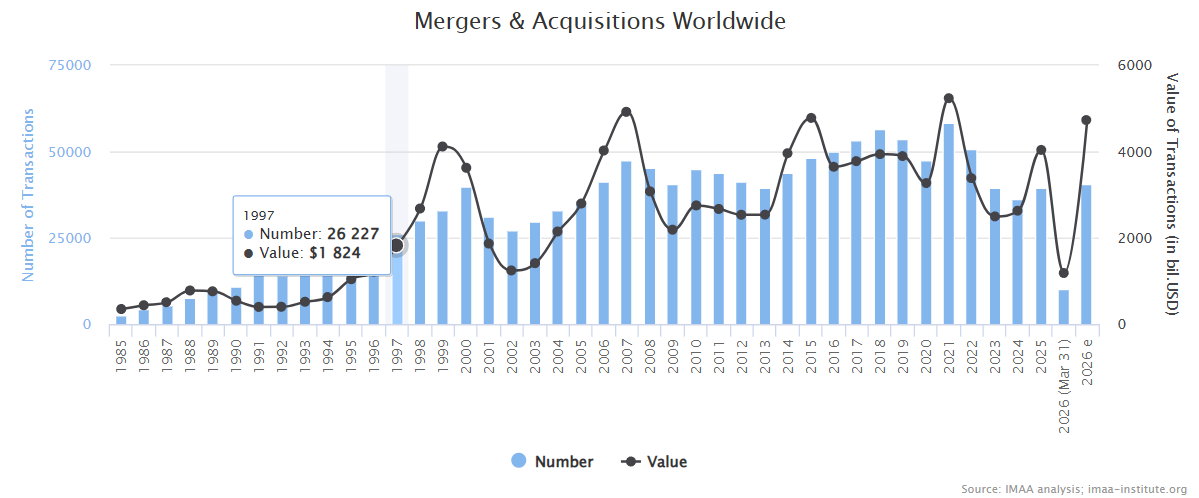
\includegraphics[width=\textwidth]{figures/ch11/mna_waves.png}
\caption{Number of transactions (bars, left axis) and value of transactions in billions of US dollars (line,
right axis) of mergers and acquisitions worldwide, 1985--2026. The 2026 entries are the first quarter and a
full-year estimate. Source: Institute for Mergers, Acquisitions and Alliances (IMAA), imaa-institute.org.}
\label{fig:11-waves}
\end{figure}

Within an industry, mergers often come in sequences that reshape the market over two or three decades.
\Cref{tab:11-consolidation} summarizes three such histories. US telecommunications went from the 1984 breakup of
AT\&T into seven regional ``Baby Bells'' to a handful of national carriers. The major US airlines consolidated
through mergers and failures after deregulation (\cref{ch:airlines}). World brewing was transformed by a chain of
very large deals between 2000 and 2012, and \cref{sec:11-millercoors} studies one of them, the MillerCoors joint
venture, in detail. \Cref{fig:11-beer} reproduces the brewing timeline.

\begin{table}[htbp]
\centering
\caption{Three consolidation histories}
\label{tab:11-consolidation}
\footnotesize
\begin{tabularx}{\textwidth}{@{}p{2.0cm}X@{}}
\toprule
Industry & Main combinations and outcome \\
\midrule
US telecom &
In 1984 AT\&T's local operations were split into seven regional companies: Ameritech, Bell Atlantic,
BellSouth, NYNEX, Pacific Telesis, Southwestern Bell and U\,S West. Southwestern Bell, renamed SBC, absorbed
Pacific Telesis (1997) and Ameritech (1999), then acquired AT\&T Corp.\ (2005) and took the name AT\&T Inc.,
and then acquired BellSouth (2006). Bell Atlantic, NYNEX and GTE formed Verizon (2000), which later absorbed MCI,
while Verizon Wireless absorbed Alltel. Qwest absorbed U\,S West and was in turn absorbed by CenturyLink.
Subscribers at the end of 2010 were: AT\&T 24 million landline and 96 million wireless, Verizon 26 million
landline and Verizon Wireless 94 million. Sprint had 50 million, T-Mobile USA 34 million and CenturyLink 15 million
landline. AT\&T's proposed \$39 billion purchase of T-Mobile USA (2011) was abandoned the same year
(\cref{tab:11-recent}). \\[3pt]
US airlines &
After deregulation in 1978, Trans World Airlines (which had absorbed Ozark) was acquired by American (2001).
Republic Airlines, itself formed from North Central, Southern and Hughes Airwest, merged into Northwest, and
Northwest merged into Delta (2008), which had absorbed Western (1987). Continental, which had absorbed People
Express among others, merged with United (2010). US Airways merged with America West (2005) and later with
American (2013). Southwest absorbed AirTran (2011). Braniff (1982), Eastern (1991) and Pan Am (1991) failed. \\[3pt]
World beer &
Interbrew and AmBev (\$11.5 billion) formed InBev (2004), which bought Anheuser-Busch for \$52 billion (2008)
to form AB InBev and later bought the rest of Grupo Modelo for \$20.1 billion. SAB bought Miller (\$5.6 billion,
2002) and later Bavaria, Grolsch and Foster's. Coors and Molson merged (2005). Heineken and Carlsberg divided the
assets of Scottish \& Newcastle (\$15.3 billion, 2008). In the United States, SABMiller and Molson Coors combined
their operations in the MillerCoors joint venture (2008). \\
\bottomrule
\end{tabularx}

\vspace{3pt}
\begin{minipage}{\textwidth}
\footnotesize Notes: Subscriber counts and the T-Mobile deal value are from a 2011 \emph{Wall Street
Journal} graphic (``A Tangled Family Tree''). Airline combinations follow the Aviation Week Intelligence
Network's Fleet Database as reproduced in the source chart, and beer deal values follow the timeline of
\cref{fig:11-beer}. Years are completion years, except the year of the proposed T-Mobile purchase. The telecom
and beer years, Western (1987) and the three airline failures are read off the time axes of these charts. The airline mergers of 2001 to 2011 are dated by
\citet[p.~11]{GAO2013}, and the 2013 merger of American and US Airways by \citet[p.~263]{AskerNocke2021}. MillerCoors
is dated by its consummation in June 2008 \citep[p.~1768]{MillerWeinberg2017}.
\end{minipage}
\end{table}

\begin{figure}[htbp]
\centering
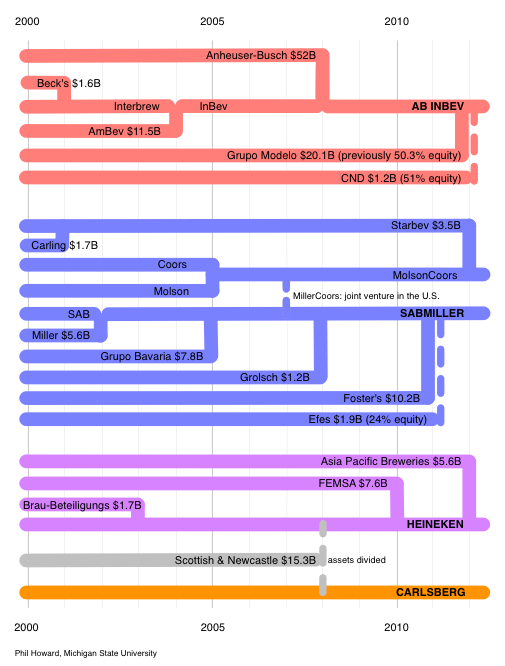
\includegraphics[width=0.5\textwidth]{figures/ch11/beer_timeline.png}
\caption{Consolidation of the world beer industry, 2000--2012. Each band is a brewer, and a band that ends in
a vertical connector is acquired by the band it joins. Labels give deal values in billions of US dollars.
Source: Phil Howard, Michigan State University, as printed on the figure.}
\label{fig:11-beer}
\end{figure}

\casehead{Two views of why firms merge}
Industrial organization economists stress three motives. The first is market power. A merger internalizes the
competition between the merging firms, which gives them a reason to raise prices even if all other firms keep
competing as before. These are the unilateral effects defined in the introduction to this chapter. A merger may
also make it easier for the remaining firms to coordinate, tacitly or explicitly, which gives rise to coordinated
effects (\cref{ch:collusion-theory}). The second motive is efficiencies. They include economies of scale and scope,
the rationalization of production and distribution across plants, and the transfer of know-how from the better-run
firm to the other. The third motive is strategic. A merger can deter entry or allow the firms to reposition their
products.

Corporate finance asks different questions. One is why mergers come in waves and why they cluster within
industries. \citet{MitchellMulherin1996} and \citet{AndradeMitchellStafford2001} attribute the clustering to
industry shocks, such as deregulation, new technologies and changes in input prices, which make a new industry
structure efficient. A second question is why the stock returns of acquirers are weak around acquisitions while
targets gain. Several theories blame agency problems or mispricing. \citet{Jensen1986} argues that managers of
firms with free cash flow overinvest in acquisitions to build empires. \citet{Roll1986} argues that overconfident
managers overpay. \citet{ShleiferVishny2003} argue that overvalued acquirers use their stock to buy undervalued
targets, so that waves follow stock-market valuations. These explanations are complements to the industrial
organization view and say little about prices. We therefore leave them aside.

The theory developed in this chapter delivers three results that will guide the empirical work. In a Cournot
market, a merger without cost savings raises the price, and it is often unprofitable for the merging firms
(\cref{sec:11-cournot}). In a symmetric market with differentiated products and price competition, every merger
is profitable (\cref{sec:11-upp}). When firms must invest in costly capacity, a merger can be profitable even
without cost savings (\cref{sec:11-beyond}).

\subsection{The legal framework and the US review process}\label{sec:11-review}

Section 7 of the Clayton Act of 1914, as amended in 1950, prohibits acquisitions whose effect ``may be
substantially to lessen competition, or to tend to create a monopoly'' \citep[p.~2]{FarrellShapiro2010}. The
word ``may'' matters. The government does not have to prove that a merger will harm competition, only that it is
likely to. Section 7 applies to every acquisition, including those that are too small to be reported and those
already consummated.

\casehead{Notification and the waiting period}
The Hart-Scott-Rodino Antitrust Improvements Act of 1976 (HSR) added Section 7A to the Clayton Act. It requires
the parties to a sufficiently large transaction to notify the Federal Trade Commission (FTC) and the Antitrust
Division of the Department of Justice (DOJ) before they close. Its motivation was the cost of undoing completed
mergers. The leading example, \emph{United States v.\ El Paso Natural Gas}, took seven years to litigate and ten
more years to carry out the divestiture the Supreme Court had ordered \citep[p.~5]{AshenfelterHosken2008}. Until
2001 every merger involving more than \$15 million in assets had to be reported. In February 2001 the threshold
rose to transactions above \$50 million and was indexed to the growth of national income, which explains much of
the fall in filings after 2001 \citep[p.~6, n.~7]{AshenfelterHosken2008}. The indexed threshold was \$63 million
in 2008 \citep[p.~2, n.~3]{FarrellShapiro2010} and \$133.9 million in 2026 \citep[p.~2134]{FTC2026}. The 2001
change also altered which mergers took place, as the end of this subsection shows.

After both parties file, a waiting period of 30 days begins (15 days for cash tender offers and bankruptcy
sales). During this period the two agencies decide which one will review the deal, a step called
\emph{clearance}. That agency then conducts a preliminary review of market shares, concentration, company
documents and complaints from customers or rivals. The agency may end the wait early through \emph{early
termination}. If the deal looks problematic, the agency issues a \emph{Second Request}, a detailed subpoena for
documents and data on competition, entry, substitution and claimed efficiencies. The waiting period then extends
until 30 days after the parties have substantially complied \citep[p.~6]{AshenfelterHosken2008}. Compliance
typically takes two or three months and sometimes six months or more. The whole investigation, with depositions
and interviews of customers and competitors, often lasts about a year.

\casehead{Outcomes}
An investigation ends in one of four ways. The agency may close it and let the merger proceed. It may negotiate
a \emph{consent decree}, usually requiring the parties to divest overlapping assets. For DOJ decrees, the Tunney
Act requires a federal court to find that the decree is in the public interest. The agency may sue to block the
merger, which in practice means seeking a preliminary injunction in federal court. Finally, the parties may
abandon the deal. The last three outcomes are counted as \emph{enforcement actions}. Much of the bargaining takes
place in the shadow of litigation. In fiscal year 2006, for example, 1,768 transactions were reported, the
agencies issued 45 Second Requests and challenged 32 transactions. The challenges led to 17 settlements, 6
restructured transactions and 9 abandoned deals \citep[p.~2, n.~5]{FarrellShapiro2010}. Some industries follow
their own rules. Rail mergers, for instance, fall under the exclusive jurisdiction of the Surface Transportation
Board. \Cref{fig:11-hsrflow} summarizes the process.

\begin{figure}[htbp]
\centering
\begin{tikzpicture}[
  box/.style={draw, rounded corners=2pt, align=center, font=\footnotesize, text width=2.2cm,
              minimum height=1.05cm, inner sep=3pt, execute at begin node={\hyphenpenalty=10000\exhyphenpenalty=10000}},
  proc/.style={box, fill=gray!8},
  dec/.style={box, fill=yellow!14},
  pass/.style={box, fill=green!9},
  stopb/.style={box, fill=red!9},
  arr/.style={-{Stealth[length=2mm]}, thin},
  lab/.style={font=\scriptsize, inner sep=1.5pt}]
\node[proc] (agree) at (0,0) {Firms agree to merge};
\node[dec]  (rep)   at (3.05,0) {Reportable under HSR? (deal above threshold)};
\node[proc] (file)  at (6.1,0) {Both parties file, FTC or DOJ takes the case};
\node[proc] (rev)   at (9.15,0) {30-day review: shares, HHI, documents, complaints};
\node[dec]  (sr)    at (12.2,0) {Second Request?};
\node[pass, text width=2.6cm] (notrep) at (3.05,-2.45) {Not reportable: close at will, still subject to
  Clayton Act Section 7};
\node[pass, text width=3.0cm] (wait) at (8.2,-2.45) {Waiting period ends, or early termination,
  then close};
\node[proc, text width=3.4cm] (deep) at (12.2,-2.45) {In-depth investigation: data, documents,
  diversion, UPP, simulation (often about one year)};
\node[pass, text width=2.3cm]  (o1) at (5.4,-5.0)  {Close investigation};
\node[proc, text width=2.3cm]  (o2) at (8.0,-5.0)  {Consent decree: divest overlaps};
\node[stopb, text width=2.3cm] (o3) at (10.6,-5.0) {Sue to block (injunction in federal court)};
\node[stopb, text width=2.3cm] (o4) at (13.2,-5.0) {Parties abandon};
\draw[arr] (agree) -- (rep);
\draw[arr] (rep) -- node[lab, above] {yes} (file);
\draw[arr] (rep) -- node[lab, right] {no} (notrep);
\draw[arr] (file) -- (rev);
\draw[arr] (rev) -- (sr);
\draw[arr] (sr.south west) -- (wait.north east);
\node[lab, anchor=north east] at (9.95,-1.15) {no (about 98\%)};
\draw[arr] (sr) -- node[lab, right] {yes (about 2\%)} (deep);
\foreach \o in {o1,o2,o3,o4} {\draw[arr] (deep.south) -- (\o.north);}
\draw[decorate, decoration={brace, mirror, amplitude=5pt}] ([yshift=-3pt]o2.south west) --
  node[below=6pt, font=\footnotesize] {enforcement actions} ([yshift=-3pt]o4.south east);
\end{tikzpicture}
\caption{From the decision to merge to closing in the United States. In fiscal year 2025 there were 2,006 HSR
filings, 41 Second Requests and 18 enforcement actions, equal to 2.0 and 0.9 percent of filings. Two of the 18
actions concerned transactions not reported under HSR.}
\label{fig:11-hsrflow}
\end{figure}

\Cref{tab:11-hsr} reports the number of filings, Second Requests and enforcement actions in each fiscal year
from 2003 to 2025, and \cref{fig:11-hsrplot} extends the series back to 1991. Three patterns stand out. Filings
fell from 4,926 in fiscal year 2000 to 1,187 in 2002 after the threshold increase, and to 716 in fiscal year 2009
during the financial crisis. They spiked in 2021 and 2022. Over 2003--2025 the agencies issued 2.6 Second Requests
and brought 2.0 enforcement actions for every 100 filings. These are annual activity ratios. An action can concern a
transaction filed in an earlier year, or one that was never reportable. The ratio is therefore not the share of a
year's filings that led to enforcement. Actions relative to filings have drifted down, from about 3 percent in
2010--2013 to about 2 percent in 2014--2020 and between 0.9 and 1.6 percent since 2021. Most mergers are never
examined closely.

\begin{table}[htbp]
\centering
\caption{Hart-Scott-Rodino filings, Second Requests and enforcement actions, fiscal years 2003--2025}
\label{tab:11-hsr}
\footnotesize
\begin{tabular}{@{}lrrrrr@{}}
\toprule
 & & & & \multicolumn{2}{c}{Ratio to filings (percent)} \\
\cmidrule(l){5-6}
Fiscal year & Filings & Second Requests & Enforcement actions & Second Requests & Enforcement actions \\
\midrule
2003 & 1,014 & 33 & 36 & 3.3 & 3.6 \\
2004 & 1,454 & 35 & 24 & 2.4 & 1.7 \\
2005 & 1,675 & 50 & 18 & 3.0 & 1.1 \\
2006 & 1,768 & 45 & 32 & 2.5 & 1.8 \\
2007 & 2,201 & 63 & 34 & 2.9 & 1.5 \\
2008 & 1,726 & 41 & 37 & 2.4 & 2.1 \\
2009 & 716 & 31 & 31 & 4.3 & 4.3 \\
2010 & 1,166 & 42 & 41 & 3.6 & 3.5 \\
2011 & 1,450 & 55 & 37 & 3.8 & 2.6 \\
2012 & 1,429 & 49 & 44 & 3.4 & 3.1 \\
2013 & 1,326 & 47 & 38 & 3.5 & 2.9 \\
2014 & 1,663 & 51 & 33 & 3.1 & 2.0 \\
2015 & 1,801 & 47 & 42 & 2.6 & 2.3 \\
2016 & 1,832 & 54 & 47 & 2.9 & 2.6 \\
2017 & 2,052 & 51 & 39 & 2.5 & 1.9 \\
2018 & 2,111 & 45 & 39 & 2.1 & 1.8 \\
2019 & 2,089 & 61 & 38 & 2.9 & 1.8 \\
2020 & 1,637 & 48 & 43 & 2.9 & 2.6 \\
2021 & 3,520 & 65 & 32 & 1.8 & 0.9 \\
2022 & 3,152 & 47 & 49 & 1.5 & 1.6 \\
2023 & 1,805 & 37 & 28 & 2.0 & 1.6 \\
2024 & 2,031 & 59 & 32 & 2.9 & 1.6 \\
2025 & 2,006 & 41 & 18 & 2.0 & 0.9 \\
\midrule
Total & 41,624 & 1,097 & 812 & 2.6 & 2.0 \\
\bottomrule
\end{tabular}

\vspace{3pt}
\begin{minipage}{0.97\textwidth}
\footnotesize Notes: Compiled from the annual HSR reports of the FTC and DOJ. Enforcement actions combine the
merger challenges of both agencies as printed in each year's joint report, using the corrected report for 2022. The
FTC later raised its 2017 count from 21 to 23, which would give 41 for that year. A report counts an action in the
year of the agency's first public action. The action can concern a transaction filed in an earlier year or one not
reportable under HSR, as did two of the 18 actions in 2025. The ratios are counts divided by filings in the same
year, so they measure annual activity. The compiled table we draw on reports Second Request rates 0.1 point higher for 2017--2020
(2.6, 2.2, 3.0 and 3.0). It probably divides by the transactions for which a Second Request could be issued. The 2003 and 2004 rows coincide with \citet[Table 1]{AshenfelterHosken2008}, and the 2006 row with
\citet[n.~5]{FarrellShapiro2010}.
\end{minipage}
\end{table}

\begin{figure}[htbp]
\centering
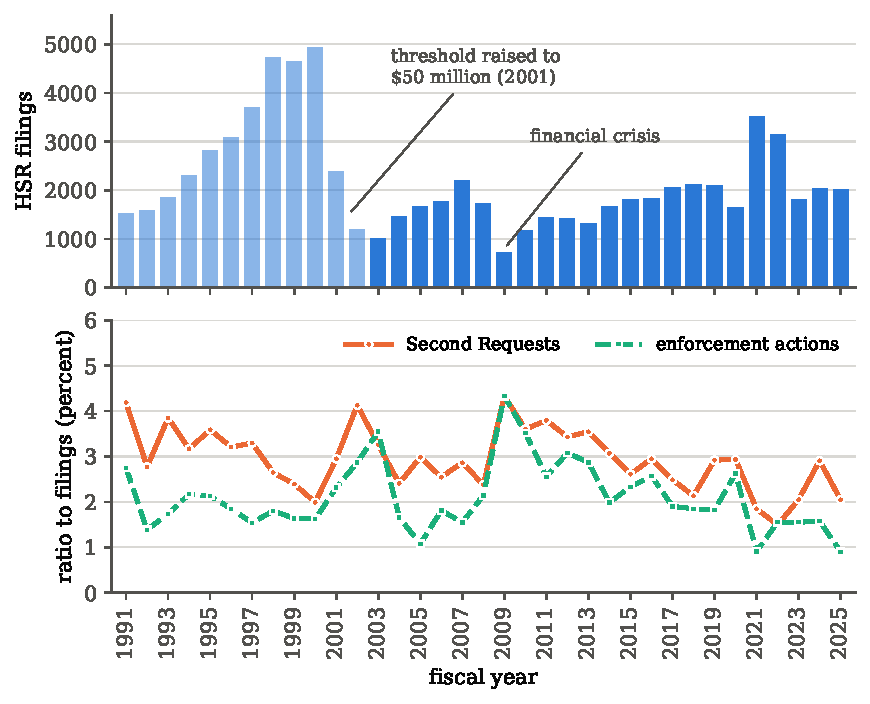
\includegraphics[width=0.86\textwidth]{figures/ch11/hsr_stats.pdf}
\caption{HSR filings (top) and the ratios of Second Requests and enforcement actions to filings in the same year, in
percent (bottom), fiscal years 1991--2025. The lighter bars for 1991--2002 come from \citet[Table 1]{AshenfelterHosken2008}, the
rest from \cref{tab:11-hsr}. Both ratios use all filings as the denominator.}
\label{fig:11-hsrplot}
\end{figure}

\casehead{Enforcement and selection}
Enforcement shapes which mergers we observe. \citet[p.~5]{AshenfelterHosken2008} report that 37,201 mergers were
filed from 1991 through 2004. About 97 percent were allowed to proceed without a full investigation. Of the 3
percent investigated in depth, roughly 65 percent were modified, abandoned or blocked.
\citet[p.~4, n.~5]{AshenfelterHoskenWeinberg2011} summarize the first figure as 97 percent of proposed mergers
going through without modification. Because the agencies try to stop the mergers most likely to raise prices,
the consummated mergers that a researcher can study are a selected sample. The average price effect of approved
mergers is a lower bound on the average effect that mergers would have in a world without enforcement
\citep{Carlton2009}. The informative object for policy is the effect of the \emph{marginal} merger, one that was
nearly blocked. \Cref{sec:11-retro} returns to this problem.

\casehead{Notification thresholds as a screen}
Reporting thresholds do more than save the agencies work. They also shape which mergers firms propose.
\citet{BesankoSpulber1993} model a review in which the merging parties know their merger-specific efficiencies and
the authority does not. Proposing a merger costs a fixed amount that cannot be recovered. Holding fixed the
probability of approval, only mergers whose efficiencies exceed a threshold are then worth proposing. A positive
proposal cost can therefore benefit consumers, because it improves the pool of proposed mergers
\citep[p.~223]{AskerNocke2021}. The same model suggests one reason why authorities apply a consumer surplus
standard rather than a total surplus standard. An authority that puts less weight on profit than society does is
tougher. It approves fewer mergers, and the proposals it receives are better as a result \citep[p.~223,
n.~120]{AskerNocke2021}.

\citet{Wollmann2019} tests this selection effect with the 2001 amendment, which raised the size-of-transaction
threshold. The agencies almost never investigated the newly exempt deals afterward, in line with the long-standing
observation that they rarely examine mergers that need not be reported. Wollmann compares newly exempt horizontal
mergers with newly exempt non-horizontal ones, which seldom raise concerns. This is a \emph{difference-in-differences}
design, which compares the change in a treated group with the change in a control group (\cref{sec:11-retro-problem}
develops it). A \emph{triple difference} also subtracts the same comparison among \emph{never-exempt} mergers, those
above the new threshold of \$50 million, which had to be reported both before and after the amendment. Newly exempt
mergers lie between the old \$15 million threshold and the new one. After
2001, never-exempt horizontal and non-horizontal mergers moved together. Newly exempt horizontal mergers rose
relative to newly exempt non-horizontal ones. The triple-difference estimate is a 50 percent increase: 324
additional newly exempt horizontal mergers per year on a pre-amendment base of 634 \citep[pp.~224--226]{AskerNocke2021}.
Through the lens of the Besanko-Spulber model, the amendment removed both the proposal cost and the risk of a
challenge for these deals. Mergers without large synergies became worth doing, so the pool of mergers grew and
worsened at the same time.

Firms also size their deals around the threshold. \citet{CunninghamEdererMa2021} study pharmaceutical acquisitions.
Acquisitions of targets whose drug projects overlap with the acquirer's bunch just below the HSR threshold, while
acquisitions without such overlap do not \citep[pp.~226--227 and Figure 9]{AskerNocke2021}. \Cref{sec:11-open}
returns to these acquisitions.

\subsection{What the agencies analyze}\label{sec:11-agencies}

The agencies' Horizontal Merger Guidelines describe five tasks \citep{USDOJFTC1992,USDOJFTC2010}, which
\citet[p.~7]{AshenfelterHosken2008} summarize. The first two
define the market. The \emph{relevant product market} is a set of close substitutes for the merging firms'
products, found with the hypothetical monopolist test of \cref{sec:11-hmt}. The \emph{relevant geographic market}
is the narrowest area in which anticompetitive effects could occur. For nationally distributed branded goods it is
typically the whole country \citep[p.~7]{AshenfelterHosken2008}. The third task is to assess competitive effects,
both unilateral and coordinated. The fourth is to evaluate efficiency claims. Efficiencies count only if they
are \emph{merger-specific}, meaning that no other arrangement that harms competition less could achieve them, and
\emph{verifiable} by the authority at the time of review \citep[p.~221]{AskerNocke2021}. They must also be large
enough to reverse the merger's potential to harm customers, for instance by preventing price increases
\citep[Section~10]{USDOJFTC2010}. The fifth is to ask whether entry would be timely, likely and sufficient to deter
or counteract the competitive effects of concern (Section~9). \Cref{sec:11-freeentry} shows what free entry implies
for the effects of a merger and how slowly entry can come in practice.
Economists at the agencies work mostly on market definition and competitive effects. The rest of this chapter
follows the same order. \Cref{sec:11-marketdef} covers market definition and concentration, and the remaining
sections cover competitive effects and efficiencies.

\casehead{Evidence on efficiencies}
The efficiency defense rests on a thin empirical base. \citet[pp.~219--221]{AskerNocke2021} single out two studies
that document merger-specific efficiencies. The first, \citet{AshenfelterHoskenWeinberg2015}, measures the
shipping savings of the MillerCoors joint venture, which \cref{sec:11-mc-assessment} discusses. The second,
\citet{BraguinskyEtAl2015}, studies 73 acquisitions in the Japanese cotton-spinning industry between 1896 and 1920.
More profitable firms bought less profitable ones, although the two groups had similar physical productivity. The
acquired mills then improved their inventory management, accounts receivable and capacity utilization, and market
power explains little of their higher profitability. The two cases illustrate the two conditions above. The beer
savings came from shorter shipping distances, which are easy to verify. The brewers might, however, have obtained
them by brewing each other's beer under contract while pricing independently, which questions their merger
specificity. The managerial gains in cotton spinning are specific to the merger but hard to verify before they
occur.

Evidence on how often mergers create efficiencies, and how large they are, is scarcer still.
\citet{GeurtsVanBiesebroeck2019} find that about 80 percent of the mergers in Belgium between 2005 and 2012 raised
employment, which may reflect higher output. \citet{GriecoPinkseSlade2018} estimate returns to scale in the
Molson-Coors merger and translate them into marginal-cost reductions \citep[pp.~221--222]{AskerNocke2021}. In the
words of \citet[p.~261]{AskerNocke2021}, not much is known about the typical magnitudes of merger efficiencies or
about how they relate to market structure.

\section{Market definition and concentration screens}\label{sec:11-marketdef}

Market shares and concentration indices are defined only relative to a market (\cref{sec:01-market-definition}).
The agencies therefore begin by defining the relevant market, and they then compute shares and the
Herfindahl-Hirschman index within it. This section derives the logic of the hypothetical monopolist test, the
algebra of critical loss, the theory behind concentration thresholds, and the reasons the whole approach struggles
with differentiated products.

\subsection{The hypothetical monopolist test}\label{sec:11-hmt}

\begin{definition}[Hypothetical monopolist test]\label{def:11-hmt}
Consider a hypothetical profit-maximizing firm that owns all products in a candidate set and faces no
regulation of its prices. Hold the terms of sale of all other products fixed. The set is a \emph{relevant product
market} if this firm would impose at least a \emph{small but significant and non-transitory increase in price}
(SSNIP) on some product of the merging firms.
\end{definition}

The SSNIP is usually 5 percent of the price and sometimes 10 percent. The test is applied iteratively. We start
from the products of the merging firms. If a hypothetical monopolist of this set would not raise price by the
SSNIP, because too many buyers would switch to products outside the set, the set is too narrow. We then add the
next-closest substitute and repeat. The relevant market is the smallest set that passes. The relevant geographic
market is defined the same way, with locations in place of products. The test turns market definition into a
statement about demand, so it can draw on the demand models of \cref{ch:aids,ch:logit,ch:blp}.

The test must be applied at the right prices. In \emph{United States v.\ E.\ I.\ du Pont de Nemours \& Co.}
(1956) the Supreme Court held that cellophane competed with other flexible wrapping materials, partly because
many buyers switched between them. Du Pont, however, already set the price of cellophane as a near monopolist. A
monopolist prices where its demand is elastic, since its Lerner condition $\frac{p - c}{p} = \frac{1}{\varepsilon}$
requires $\varepsilon > 1$. At monopoly prices, almost any product looks like it has close substitutes. Applying
the test at prices that already reflect market power therefore yields markets that are too broad. This error is
called the \emph{cellophane fallacy}. In merger review the problem is milder, because the question is whether the
merger would raise prices above their current level.

\subsection{Critical loss analysis}\label{sec:11-critloss}

\emph{Critical loss analysis} turns the hypothetical monopolist test into a comparison of two numbers. Consider a
hypothetical monopolist of the candidate set that sells quantity $q$ at price $p$, with constant marginal cost
$c$ and percentage margin $L = \frac{p - c}{p}$. Suppose it raises the price by a fraction $X$ to $p(1 + X)$, and
let $\mathit{AL}$ be the resulting \emph{actual loss}, the fraction of unit sales lost. Profit before the increase is
\begin{equation*}
(p - c)\,q = L\,pq.
\end{equation*}
Profit after the increase is
\begin{align*}
\big(p(1 + X) - c\big)\,q\,(1 - \mathit{AL})
&= \big(pX + (p - c)\big)\,q\,(1 - \mathit{AL}) \\
&= (X + L)(1 - \mathit{AL})\,pq.
\end{align*}
Profit per dollar of pre-merger revenue therefore moves from $L$ to $(X + L)(1 - \mathit{AL})$. The increase is
profitable if and only if
\begin{align}
(X + L)(1 - \mathit{AL}) &\ge L \notag \\
\iff X + L - (X + L)\,\mathit{AL} &\ge L \notag \\
\iff \mathit{AL} &\le \frac{X}{X + L} \equiv \mathit{CL}. \label{eq:11-cl}
\end{align}
The number $\mathit{CL}$ is the \emph{critical loss}, the largest loss of sales that leaves the price increase
profitable. With $X = 0.05$ and $L = 0.4$, the critical loss is $\frac{0.05}{0.45} = 11.1$ percent.

\casehead{From critical loss to a threshold elasticity}
The actual loss depends on the shape of demand. With linear demand $q(p) = d_0 - d_1 p$, the quantity
falls by $d_1 pX$, so
\begin{equation*}
\mathit{AL} = \frac{d_1 pX}{q} = \varepsilon X,
\end{equation*}
where $\varepsilon = \frac{d_1 p}{q}$ is the elasticity of the candidate market's demand at the initial
price. Substituting into \eqref{eq:11-cl}, the SSNIP breaks even if and only if
\begin{equation}\label{eq:11-ce-lin}
\varepsilon \le \frac{1}{X + L}.
\end{equation}
We call the right side the breakeven \emph{threshold elasticity}. The test in \eqref{eq:11-cl} asks whether a price increase of $X$ is \emph{profitable}. The Guidelines ask whether
the monopolist \emph{would impose} it, which is the stronger requirement that the profit-maximizing increase be
at least $X$. With linear demand, profit after an increase $x$ is
\begin{equation*}
\pi(x) = (x + L)(1 - \varepsilon x)\,pq,
\end{equation*}
which is concave in $x$. Its derivative is
\begin{equation*}
\pi'(x) = \big[(1 - \varepsilon x) - \varepsilon (x + L)\big]\,pq = (1 - 2\varepsilon x - \varepsilon L)\,pq.
\end{equation*}
By concavity, the optimal increase is at least $X$ if and only if $\pi'(X) \ge 0$, that is,
\begin{equation}\label{eq:11-ce-lin-pm}
\varepsilon \le \frac{1}{2X + L}.
\end{equation}
This bound is tighter than \eqref{eq:11-ce-lin}. With constant-elasticity demand $q(p) = A p^{-\varepsilon}$ the
loss is $\mathit{AL} = 1 - (1 + X)^{-\varepsilon}$. The breakeven condition becomes
$(X + L)(1 + X)^{-\varepsilon} \ge L$, or
\begin{equation*}
\varepsilon \le \frac{\ln\!\big(\frac{X + L}{L}\big)}{\ln(1 + X)}.
\end{equation*}
For the profit-maximizing version, the monopoly price with constant elasticity $\varepsilon > 1$ is
$\frac{\varepsilon}{\varepsilon - 1}c$, and $c = (1 - L)p$. The optimal increase is at least $X$ if and only if
$\frac{\varepsilon}{\varepsilon - 1}(1 - L) \ge 1 + X$, which rearranges to
$\varepsilon \le \frac{1 + X}{X + L}$.

\Cref{tab:11-critloss} reports these thresholds. Two lessons emerge. First, the critical loss falls steeply as the
margin rises. Second, the threshold elasticity depends on the curvature of demand. With $X = 0.05$ and $L = 0.4$, a
market elasticity of 2.2 passes the breakeven test under both demand curves. It fails the profit-maximizing test
under linear demand and passes it under constant elasticity. Market definition thus depends on curvature, and
hence on pass-through (\cref{sec:02-passthrough}), a point we return to in \cref{sec:11-diffmarkets}.

\begin{table}[htbp]
\centering
\caption{Critical loss and the threshold elasticity of market demand}
\label{tab:11-critloss}
\footnotesize
\begin{tabular}{@{}cccccccc@{}}
\toprule
 & & & \multicolumn{2}{c}{Linear demand} & & \multicolumn{2}{c}{Constant elasticity} \\
\cmidrule{4-5} \cmidrule{7-8}
\makecell{SSNIP\\$X$} & \makecell{Margin\\$L$} & \makecell{Critical loss\\$\mathit{CL}$ (\%)} & Breakeven &
\makecell{Profit-\\maximizing} & & Breakeven & \makecell{Profit-\\maximizing} \\
\midrule
0.05 & 0.2 & 20.0 & 4.00 & 3.33 & & 4.57 & 4.20 \\
0.05 & 0.4 & 11.1 & 2.22 & 2.00 & & 2.41 & 2.33 \\
0.05 & 0.6 & \phantom{0}7.7 & 1.54 & 1.43 & & 1.64 & 1.62 \\
0.10 & 0.2 & 33.3 & 3.33 & 2.50 & & 4.25 & 3.67 \\
0.10 & 0.4 & 20.0 & 2.00 & 1.67 & & 2.34 & 2.20 \\
0.10 & 0.6 & 14.3 & 1.43 & 1.25 & & 1.62 & 1.57 \\
\bottomrule
\end{tabular}

\vspace{3pt}
\begin{minipage}{0.97\textwidth}
\footnotesize Notes: The SSNIP passes if the elasticity of the candidate market's demand is at most the entry
shown. Linear demand: $\frac{1}{X + L}$ (breakeven) and $\frac{1}{2X + L}$ (profit-maximizing). Constant
elasticity: $\frac{\ln\left(\frac{X + L}{L}\right)}{\ln(1 + X)}$ (breakeven) and $\frac{1 + X}{X + L}$
(profit-maximizing).
\end{minipage}
\end{table}

\casehead{The critical loss paradox and aggregate diversion}
High margins make the critical loss small. Merging parties have used this to argue for broad markets. With a
40 percent margin, they say, losing just 11 percent of sales makes a 5 percent increase unprofitable, and surely
more buyers than that would switch. \citet{KatzShapiro2003} and \citet{OBrienWickelgren2003} point out the flaw. High
margins are not exogenous. Before the merger, each firm in the candidate market sets its own price, so its own
demand elasticity equals the inverse of its margin. A high margin therefore signals that each firm faces less elastic
demand and loses fewer sales when it raises its price alone. What matters for the hypothetical monopolist is where
those sales go. Sales diverted to other products in the candidate market are recaptured by the monopolist.

To make this precise, we use the diversion ratio $D_{jk}$ of \cref{def:04-diversion}, the fraction of the sales that
$j$ loses when its price rises that go to $k$. The aggregate diversion ratio of $j$ to a set of products sums its
diversion ratios to the members of the set (\cref{def:11-aggdiv}).

\begin{proposition}[Critical loss and aggregate diversion, \citealp{KatzShapiro2003}]\label{prop:11-aggdiv}
Consider a candidate market of $n$ symmetric products, each sold by a single-product firm at price $p$ with
marginal cost $c$ and margin $L = \frac{p - c}{p}$. Assume pre-merger prices satisfy each firm's first-order
condition, and demand is linear over the relevant range. Let $\bar D$ be each product's aggregate diversion
ratio to the other $n - 1$ products. A uniform price increase $X$ on all $n$ products causes the actual loss
\begin{equation}\label{eq:11-al-div}
\mathit{AL} = \frac{X(1 - \bar D)}{L},
\end{equation}
and the increase is profitable for a hypothetical monopolist if and only if
\begin{equation}\label{eq:11-aggdiv}
\bar D \ge \frac{X}{X + L} = \mathit{CL}.
\end{equation}
\end{proposition}

\begin{proof}
Write $\varepsilon_{jj} = -\frac{\partial q_j}{\partial p_j}\frac{p}{q_j}$ for the own elasticity of product $j$.
Its firm's first-order condition gives the Lerner condition $L = \frac{1}{\varepsilon_{jj}}$. When all prices rise
by $pX$, linearity gives the change in $q_j$ as
\begin{equation*}
\Delta q_j = \frac{\partial q_j}{\partial p_j}\,pX + \sum_{k \ne j}\frac{\partial q_j}{\partial p_k}\,pX.
\end{equation*}
By symmetry of the products, $\frac{\partial q_j}{\partial p_k} = \frac{\partial q_k}{\partial p_j}$, and the
definition of diversion gives
\begin{equation*}
\sum_{k \ne j}\frac{\partial q_j}{\partial p_k} = \sum_{k \ne j}\frac{\partial q_k}{\partial p_j}
= -\bar D\,\frac{\partial q_j}{\partial p_j}.
\end{equation*}
Substituting,
\begin{equation*}
\Delta q_j = \frac{\partial q_j}{\partial p_j}\,pX\,(1 - \bar D),
\qquad
\mathit{AL} = -\frac{\Delta q_j}{q_j} = \varepsilon_{jj}X(1 - \bar D) = \frac{X(1 - \bar D)}{L}.
\end{equation*}
This is \eqref{eq:11-al-div}. By \eqref{eq:11-cl} the increase is profitable if and only if
$\frac{X(1 - \bar D)}{L} \le \frac{X}{X + L}$. Multiplying by $\frac{L(X + L)}{X} > 0$ gives
$(1 - \bar D)(X + L) \le L$, which rearranges to $X \le \bar D(X + L)$, that is, $\bar D \ge \frac{X}{X + L}$.
\end{proof}

\Cref{prop:11-aggdiv} reverses the paradox. A single firm that raised its price alone would lose
$\frac{X}{L}$ of its sales, which always exceeds $\mathit{CL} = \frac{X}{X + L}$. The hypothetical monopolist loses only
the part that leaves the candidate market. With $L = 0.4$ and $X = 0.05$, it suffices that 11.1 percent of the
sales lost by each product are recaptured by the others. High margins thus make narrow markets more likely,
because the hurdle $\mathit{CL}$ falls while diversion is unchanged. Analyses that estimate the hypothetical
monopolist's actual loss from single-firm elasticities ignore recapture. Some such analyses have concluded that a
hypothetical monopolist would want to cut price below pre-merger levels, which contradicts the premise that
pre-merger prices maximize each firm's profit \citep[p.~25, n.~74]{FarrellShapiro2010}. The uniform price
increase in \cref{prop:11-aggdiv} is a simplification, since the test only requires an increase on one product of
the merging firms.

\citet[Appendix]{FarrellShapiro2010} use the same logic to link market definition to diversion between the
merging products. In a candidate market that exactly meets the breakeven test, the aggregate diversion ratio of
each product equals $\frac{X}{L + X}$. If diversion within the market is proportional to market shares $s_k$, the
diversion from product 1 to product 2 is
\begin{equation}\label{eq:11-fs-proxy}
D_{12} = \frac{s_2}{1 - s_1}\cdot\frac{X}{L + X}.
\end{equation}
\Cref{sec:11-upp} uses diversion ratios of this kind directly, without defining a market.

\subsection{Concentration measures and the Guidelines}\label{sec:11-hhi}

Once a market is defined, the agencies compute the Herfindahl-Hirschman index $\HHI = \sum_i s_i^2$ of
\cref{def:01-concentration}, reported in HHI points ($10{,}000 \times \HHI$, or shares in percent squared). If
firms $A$ and $B$ merge and the merged firm keeps their combined share, the index changes by
\begin{align}
\Delta\HHI &= (s_A + s_B)^2 - s_A^2 - s_B^2 \notag \\
&= s_A^2 + 2 s_A s_B + s_B^2 - s_A^2 - s_B^2 \notag \\
&= 2 s_A s_B. \label{eq:11-dhhi}
\end{align}
The Guidelines classify mergers by the post-merger index and by this change. \Cref{tab:11-guidelines} compares
the thresholds of the 1992 and 2010 Horizontal Merger Guidelines and the 2023 Merger Guidelines.

\begin{table}[htbp]
\centering
\caption{Concentration thresholds in the US merger guidelines}
\label{tab:11-guidelines}
\footnotesize
\begin{tabularx}{\textwidth}{@{}>{\raggedright\arraybackslash}p{2.3cm}*{3}{>{\raggedright\arraybackslash}X}@{}}
\toprule
 & 1992 Horizontal Merger Guidelines & 2010 Horizontal Merger Guidelines & 2023 Merger Guidelines \\
\midrule
Market categories (post-merger HHI) &
Unconcentrated below 1,000, moderately concentrated from 1,000 to 1,800, highly concentrated above 1,800 &
Unconcentrated below 1,500, moderately concentrated from 1,500 to 2,500, highly concentrated above 2,500 &
Highly concentrated above 1,800 \\[3pt]
Safe harbors &
Unconcentrated markets, and $\Delta\HHI < 100$ (moderately concentrated) or $\Delta\HHI < 50$ (highly
concentrated) &
Unconcentrated markets, and $\Delta\HHI < 100$ in any market &
No explicit safe harbor \\[3pt]
Potential concern &
$\Delta\HHI > 100$ in moderately concentrated markets, and $\Delta\HHI$ from 50 to 100 in highly
concentrated markets &
$\Delta\HHI > 100$ in moderately concentrated markets, and $\Delta\HHI$ from 100 to 200 in highly concentrated
markets &
\\[3pt]
Presumption of harm &
Post-merger HHI above 1,800 and $\Delta\HHI > 100$ &
Post-merger HHI above 2,500 and $\Delta\HHI > 200$ &
Post-merger HHI above 1,800 and $\Delta\HHI > 100$, or a merged firm with a share above 30 percent and
$\Delta\HHI > 100$ \\
\bottomrule
\end{tabularx}

\vspace{3pt}
\begin{minipage}{\textwidth}
\footnotesize Notes: HHI points (shares in percent). The 1992 presumption is quoted from Section 1.51 in
\citet[p.~11, n.~25]{AshenfelterHosken2008} and \citet[p.~26]{FarrellShapiro2010}. The other 1992 entries are the
boundaries of 1,000 and 1,800 and the thresholds of 100 and 50 points. They coincide with the screen of the 1982 and
1984 Guidelines as \citet[pp.~5--6]{Nevo2000b} describes it. Sources: \citet[Section~1.51]{USDOJFTC1992},
\citet[Section~5.3]{USDOJFTC2010} and \citet[Section~2.1]{USDOJFTC2023}. The 2023 Guidelines contain no safe harbor.
\end{minipage}
\end{table}

\casehead{Why concentration}
The theoretical case for concentration screens comes from Cournot competition. With homogeneous goods and
constant marginal costs, firm $i$'s first-order condition $P + q_i P'(Q) = c_i$ implies
$\frac{P - c_i}{P} = \frac{s_i}{\varepsilon}$. Weighting by shares and summing gives the share-weighted Lerner
index $\frac{\HHI}{\varepsilon}$ \citep{CowlingWaterson1976}, as \cref{prop:01-cowling-waterson} shows. A higher
share lowers a firm's marginal revenue, and concentration summarizes this force for the industry
\citep[p.~3]{FarrellShapiro2010}. The formula $\Delta\HHI = 2 s_A s_B$, however, assumes that the merged firm keeps
the combined share. \citet[p.~2]{FarrellShapiro1988} note that this assumption is self-defeating. If all firms
kept their outputs, the merger would affect neither consumers nor rivals. Once outputs respond, the formula is
wrong.

\begin{example}[Naive and equilibrium changes in concentration]\label{ex:11-naivehhi}
Consider $N$ symmetric Cournot firms with constant marginal cost, and suppose two of them merge without cost
savings. The merged firm is then just another symmetric firm, so the post-merger equilibrium has $N - 1$
symmetric firms. The equilibrium change and the naive change in the index are
\begin{equation*}
\Delta\HHI = \frac{1}{N - 1} - \frac{1}{N} = \frac{1}{N(N - 1)},
\qquad
2 s_A s_B = \frac{2}{N^2}.
\end{equation*}
The ratio of the naive change to the equilibrium change is $\frac{2(N - 1)}{N}$, which exceeds one whenever
$N > 2$. The naive formula overstates the change
in concentration because the merged firm contracts and the outsiders expand. For a symmetric seven-to-six merger,
the naive calculation raises the index from 1,429 to 1,837, an increase of 408 points
\citep[p.~26]{FarrellShapiro2010}. Six symmetric firms, however, have an index of 1,667, so the equilibrium
increase is 238 points. The naive numbers trigger the presumption of the 1992 and 2023 Guidelines. The
equilibrium numbers trigger neither. Moreover, \cref{sec:11-ssr} shows that this merger would be unprofitable in
Cournot without cost savings, so it would not be proposed in the first place. \Cref{app:problems} works through
the same calculations in a Cournot exercise.
\end{example}

\casehead{Newer foundations for the screens}
Recent theory gives the naive change $2s_As_B$ a firmer foundation than the Cowling-Waterson formula does.
\citet{NockeSchutz2019} study multiproduct firms that compete in prices under logit, nested logit or CES demand.
Without merger-specific efficiencies, the losses of consumer surplus and of aggregate surplus caused by a merger are
both approximately proportional to the naive $\Delta\HHI$. The approximation is taken around small market shares
\citep[p.~226]{AskerNocke2021}. \citet{NockeWhinston2020} ask how large the efficiencies must be for a merger not to
harm consumers. They also ask how the answer depends on the change and on the level of the index. They answer in theory for
Cournot competition with homogeneous goods and for price competition with logit and CES demand. They also answer
empirically for hypothetical mergers in the US beer industry, using the demand and cost estimates of
\citet{MillerWeinberg2017}. The required efficiencies
rise with the naive $\Delta\HHI$ and, holding it fixed, do not depend on the level of the index
\citep[p.~227]{AskerNocke2021}. The results favor screens based on the change in concentration over screens based
on its level. Nocke and Whinston also argue that the presumptions of the 2010 Guidelines are likely too lax unless
the typical merger is credited with large synergies (n.~124). The level regains a role if the agency tolerates a
small loss of consumer surplus. The efficiency needed to keep the loss below a given small fraction rises with the
level of the index, holding its change fixed (n.~125). \Cref{sec:11-fs} derives the Cournot version of the required
efficiency, and \cref{sec:11-policy} gives a further reason to screen on naive concentration.

\casehead{A worked example}
\citet[Table 2]{AshenfelterHosken2008} report the pre-merger shares, the post-merger index and its change for five
consumer-product mergers. \Cref{tab:11-ahhhi} recomputes the change from the rounded shares. The recomputed values
are within 20 points of the reported ones. The gaps come from rounding. For General Mills and Ralcorp, for
instance, shares in $[27.5, 28.5)$ and $[3.5, 4.5)$ give $2 s_A s_B$ anywhere in $[192.5, 256.5)$, an interval
that contains the reported 238. The same check works for the other four mergers. The authors treat the combined
private-label share as one participant \citep[p.~11, n.~24]{AshenfelterHosken2008}.

\begin{table}[htbp]
\centering
\caption{Recomputing the change in concentration for five consumer-product mergers}
\label{tab:11-ahhhi}
\footnotesize
\begin{tabular}{@{}lllrrrr@{}}
\toprule
Industry & Firm $A$ & Firm $B$ & $s_A$ (\%) & $s_B$ (\%) & $2 s_A s_B$ & \makecell{Reported\\$\Delta\HHI$} \\
\midrule
Cereal & General Mills & Ralcorp (Chex) & 28 & 4 & 224 & 238 \\
Liquor & Guinness & Grand Metropolitan & 21 & 22 & 924 & 935 \\
Motor oil & Pennzoil & Quaker State & 29 & 9 & 522 & 517 \\
Feminine protection & Procter \& Gamble & Tambrands & 25 & 19 & 950 & 959 \\
Pancake syrup & Aurora Foods & Log Cabin & 15 & 19 & 570 & 589 \\
\bottomrule
\end{tabular}

\vspace{3pt}
\begin{minipage}{0.97\textwidth}
\footnotesize Notes: Shares are pre-merger revenue shares from scanner data of Information Resources Inc.\ (IRI). Post-merger HHIs reported in
the source are 2,357, 2,026, 2,189, 2,815 and 1,990. Aurora Foods (Mrs.\ Butterworth's) bought the Log Cabin
business from Philip Morris (Kraft). Guinness and Grand Metropolitan combined their spirits businesses. In the other
three mergers firm $A$ bought firm $B$'s brands. Source: \citet[Table 2]{AshenfelterHosken2008}.
\end{minipage}
\end{table}

\subsection{Why market definition struggles with differentiated products}\label{sec:11-diffmarkets}

The structural presumption has deep roots in US law. In \emph{United States v.\ Philadelphia National Bank}
(1963), the Supreme Court considered a merger that creates a firm with ``an undue percentage share of the
relevant market'' and raises concentration significantly. It held that such a merger is ``so inherently
likely to lessen competition substantially that it must be enjoined'' unless the parties show otherwise
\citep[p.~4]{FarrellShapiro2010}. The
presumption fits a homogeneous-goods market with clear boundaries. It fits poorly when products are
differentiated.

With differentiated products, any boundary is a line drawn through a chain of substitutes, and products are
either in or out. \citet[p.~5]{FarrellShapiro2010} ask whether the relevant market for the Miller and Coors
combination was domestic beer, all beer, all alcoholic beverages, or all beverages. Courts tend to define
markets broadly, including all products ``reasonably interchangeable by consumers for the same purposes''. The
hypothetical monopolist test with high margins often implies narrow markets instead. The binary choice also fits
badly with what matters for unilateral effects, which is how close the merging products are to each other.

The proposed merger of Whole Foods and Wild Oats in 2007 illustrates the problem. The two chains specialized in
natural and organic groceries. Whole Foods planned to close Wild Oats stores near its own. Its internal projections
suggested that most customers of a closed Wild Oats store would switch to Whole Foods rather than to conventional
supermarkets. Its chief executive told his board that buying Wild Oats would ``avoid nasty price wars'', and he stated
that ``one of the motivations is to eliminate a competitor'' \citep[pp.~5--6]{FarrellShapiro2010}. To invoke the structural presumption, the FTC had to define a market. It
proposed ``premium natural and organic supermarkets''. The District Court rejected this market because shoppers
also bought organic food at conventional supermarkets. The FTC appealed and won a remand. The litigation forced a
choice between two answers, a near monopoly or two small players among all supermarkets, when the economics
pointed to substantial but incomplete differentiation. In the Oracle and PeopleSoft case, the DOJ showed that the
two firms competed head to head in high-function human resources and financial management software. There the
merger would have reduced the number of major suppliers from three to two. The court found that the DOJ had not
established its market, and the merger went ahead \citep[p.~6, n.~19]{FarrellShapiro2010}.

Market definition also has a hidden dependence on demand curvature. The hypothetical monopolist test is close to
simulating a merger of all products in the candidate market. Its outcome therefore depends on pass-through in the
same way as a merger simulation \citep[p.~25]{FarrellShapiro2010}. \Cref{tab:11-critloss} showed the same dependence
in the simplest case. These problems motivate the approach of \cref{sec:11-upp}, which measures the pricing
pressure created by a merger directly from margins and diversion ratios.

\section{Unilateral effects with homogeneous goods}\label{sec:11-cournot}

This section studies mergers in markets for a homogeneous good. We begin with the trade-off between market power
and cost savings. We then show that mergers without cost savings are often unprofitable in Cournot markets. Next
comes the equilibrium analysis of \citet{FarrellShapiro1990}, which links private profitability, prices and
welfare. We end by asking what free entry changes.

\subsection{The Williamson trade-off}\label{sec:11-williamson}

\citet{Williamson1968} framed the basic question of merger policy as a trade-off. Suppose an industry is
competitive before the merger, so that the price equals unit cost, $p_0 = c_0$, and output is $q_0 = Q(p_0)$.
The merger creates market power, so the price rises to $p_1 > p_0$ and output falls to $q_1 = Q(p_1)$. It also
lowers unit cost to $c_1 < c_0$. \Cref{fig:11-williamson} shows the two effects.

\begin{figure}[htbp]
\centering
\begin{tikzpicture}[x=1.3cm, y=1.0cm, font=\small]
  \fill[gray!14] (0,2) rectangle (2.1,2.9);
  \fill[pattern=north east lines, pattern color=black!55] (0,1.4) rectangle (2.1,2);
  \fill[gray!45] (2.1,2.9) -- (2.1,2) -- (3,2) -- cycle;
  \draw[->] (0,0) -- (5.6,0) node[below] {$Q$};
  \draw[->] (0,0) -- (0,5.5) node[left] {$p$};
  \draw[thick] (0,5) -- (5,0) node[pos=0.93, above right] {$Q(p)$};
  \draw (0,2) -- (5.2,2) node[right] {$c_0$};
  \draw[dashed] (0,1.4) -- (5.2,1.4) node[right] {$c_1$};
  \draw[dashed] (0,2.9) -- (2.1,2.9);
  \draw[dotted] (2.1,2.9) -- (2.1,0) node[below] {$q_1$};
  \draw[dotted] (3,2) -- (3,0) node[below] {$q_0$};
  \node[left] at (0,2.9) {$p_1$};
  \node[left] at (0,2) {$p_0$};
  \node at (1.05,2.45) {\footnotesize transfer};
  \node[fill=white, inner sep=1pt] at (1.05,1.7) {$A_2$};
  \node at (2.38,2.27) {$A_1$};
\end{tikzpicture}
\caption{The Williamson trade-off. The merger raises the price from $p_0 = c_0$ to $p_1$ and lowers unit cost
from $c_0$ to $c_1$. The dark triangle $A_1$ is the deadweight loss. The hatched rectangle $A_2$ is the cost
saving on the remaining output $q_1$. The light rectangle is a transfer from consumers to the merged firm.}
\label{fig:11-williamson}
\end{figure}

Total surplus is consumer surplus plus profit. Approximate demand by a straight line between the two points. The
change in consumer surplus is
\begin{equation*}
\Delta CS = -\int_{p_0}^{p_1} Q(p)\,\dd p = -(p_1 - p_0)\,q_1 - \frac{1}{2}(p_1 - p_0)(q_0 - q_1).
\end{equation*}
Profit is zero before the merger. After it, profit is
\begin{align*}
\Delta\pi = (p_1 - c_1)\,q_1
&= \big[(p_1 - p_0) + (p_0 - c_1)\big]\,q_1 \\
&= (p_1 - p_0)\,q_1 + (c_0 - c_1)\,q_1,
\end{align*}
where the second line uses $p_0 = c_0$. The rectangle $(p_1 - p_0)q_1$ appears in both changes with opposite
signs. Adding them,
\begin{equation}\label{eq:11-williamson}
\Delta W = \underbrace{(c_0 - c_1)\,q_1}_{A_2} - \underbrace{\frac{1}{2}(p_1 - p_0)(q_0 - q_1)}_{A_1}.
\end{equation}

\casehead{How large must the cost saving be}
Set $\Delta W = 0$ and divide \eqref{eq:11-williamson} by $c_0 q_1 = p_0 q_1$:
\begin{equation*}
\frac{c_0 - c_1}{c_0} = \frac{1}{2}\cdot\frac{p_1 - p_0}{p_0}\cdot\frac{q_0 - q_1}{q_1}.
\end{equation*}
With a linear demand curve of elasticity $\varepsilon$ at $p_0$, the output loss is
$q_0 - q_1 = \varepsilon\,\frac{\Delta p}{p_0}\,q_0$, where $\Delta p = p_1 - p_0$. Substituting, and using
$q_1 = q_0\big(1 - \varepsilon\frac{\Delta p}{p_0}\big)$,
\begin{equation}\label{eq:11-williamson-saving}
\frac{c_0 - c_1}{c_0} = \frac{\varepsilon\big(\frac{\Delta p}{p_0}\big)^2}{2\big(1 - \varepsilon\frac{\Delta p}{p_0}\big)}
\approx \frac{1}{2}\,\varepsilon\Big(\frac{\Delta p}{p_0}\Big)^2.
\end{equation}
The approximation drops a term of third order in $\frac{\Delta p}{p_0}$. The breakeven cost saving is second order
in the price increase, because the deadweight loss is a triangle while the cost saving is a rectangle. With unit
elasticity, a 10 percent price increase is offset by a cost saving of about 0.5 percent (0.56 percent with the
exact formula). A 5 percent increase needs about 0.13 percent. With an elasticity of 2 and a 10 percent price
increase, the saving must be about 1 percent (1.25 percent exactly). Williamson concluded that modest cost savings
can offset sizable price increases under a total surplus standard.

\casehead{Welfare standards}
The conclusion depends on counting the transfer $(p_1 - p_0)q_1$ as neutral. Under a \emph{total surplus
standard}, the agency approves a merger that raises the sum of consumer and producer surplus. Under a
\emph{consumer surplus standard}, it approves only mergers that do not harm consumers, which in this setting
means the price must not rise. Antitrust authorities by and large apply the second standard
\citep[p.~223, n.~120]{AskerNocke2021}. Under the 2010 Guidelines, efficiencies save a merger only if they would
reverse its potential to harm customers, for instance by preventing price increases \citep[Section~10]{USDOJFTC2010}.
A consumer surplus standard can serve a total surplus objective, because a tougher authority induces a better pool
of proposed mergers (\cref{sec:11-review}).
Under a consumer surplus standard the trade-off disappears, and the required cost saving is much larger. Suppose demand is $P(Q) = a - bQ$ and the merged firm becomes a monopolist with cost $c_1$.
It charges $\frac{a + c_1}{2}$, which does not exceed $p_0 = c_0$ if and only if
$c_1 \le 2c_0 - a = c_0 - (a - c_0)$. Marginal cost must therefore fall by at least $a - c_0 > 0$, the gap between
the demand intercept and the initial price.

\casehead{Pre-existing market power}
If the industry already had market power, so that $p_0 > c_0$, the lost output was worth more than its cost. The
same steps, now with $\Delta\pi = (p_1 - c_1)q_1 - (p_0 - c_0)q_0$, give
\begin{equation}\label{eq:11-williamson-mp}
\Delta W = (c_0 - c_1)\,q_1 - \frac{1}{2}(p_1 - p_0)(q_0 - q_1) - (p_0 - c_0)(q_0 - q_1).
\end{equation}
The extra rectangle $(p_0 - c_0)(q_0 - q_1)$ is first order in the price increase, so in an industry that is
already concentrated, a given price increase requires a much larger cost saving.

The Williamson calculation treats the cost saving and the price increase as separate primitives. It does not ask
how the nature of the merger links the two \citep[p.~1, n.~1]{FarrellShapiro1988}. In an oligopoly, the price
effect itself depends on the cost saving and on how rivals respond. The rest of this section builds that link.

\subsection{The merger paradox}\label{sec:11-ssr}

\citet{SalantSwitzerReynolds1983} studied mergers in the simplest Cournot model and found that most of them
reduce the merging firms' profits. Let inverse demand be $P(Q) = a - Q$ and let $N$ firms have the same constant
marginal cost $c < a$. With $n$ active symmetric firms, the Cournot equilibrium (\cref{ch:theory}) has
\begin{equation*}
q = \frac{a - c}{n + 1}, \qquad P = \frac{a + nc}{n + 1}, \qquad \pi = \frac{(a - c)^2}{(n + 1)^2}.
\end{equation*}
A merger of $M$ firms, $2 \le M \le N$, without cost savings leaves $N - M + 1$ symmetric firms, because the
merged firm has the same cost as every other firm. Here $M$ counts the merging firms. Market size plays no role in
this section.

\begin{proposition}[The merger paradox, \citealp{SalantSwitzerReynolds1983}]\label{prop:11-ssr}
In the linear Cournot model with $N$ symmetric firms and constant marginal cost, a merger of $M$ firms without
cost savings raises the price and the profit of every outsider. It is profitable for the merging firms if and only
if
\begin{equation}\label{eq:11-ssr}
\frac{1}{(N - M + 2)^2} \ge \frac{M}{(N + 1)^2}.
\end{equation}
A merger of two firms is profitable only if $N = 2$. A merger to monopoly ($M = N$) is always profitable.
\end{proposition}

\begin{proof}
After the merger there are $n = N - M + 1$ firms, so $n + 1 = N - M + 2$. The price rises from
$\frac{a + Nc}{N + 1}$ to $\frac{a + (N - M + 1)c}{N - M + 2}$, since $P = c + \frac{a - c}{n + 1}$ decreases in $n$.
Each outsider's profit rises from $\frac{(a - c)^2}{(N + 1)^2}$ to $\frac{(a - c)^2}{(N - M + 2)^2}$. The merged
firm earns $\frac{(a - c)^2}{(N - M + 2)^2}$, and the $M$ insiders earned $\frac{M(a - c)^2}{(N + 1)^2}$ together
before the merger. Comparing the two gives \eqref{eq:11-ssr}. For $M = 2$ the condition reads $(N + 1)^2 \ge 2N^2$,
or $N + 1 \ge \sqrt{2}\,N$, that is,
\begin{equation*}
N \le \frac{1}{\sqrt 2 - 1} = 1 + \sqrt 2 \approx 2.41.
\end{equation*}
Only $N = 2$ satisfies it. For $M = N$ the condition reads $(N + 1)^2 \ge 4N$, or $(N - 1)^2 \ge 0$, which always
holds.
\end{proof}

How large must a merger be to pay? For $N = 5$ the smallest profitable merger has $M = 4$, which exactly breaks
even. For $N = 10$ it has $M = 9$, and for $N = 20$ it has $M = 17$. Among all $N$ up to 1,000, the smallest
profitable merger never includes fewer than 80 percent of the firms. The fraction is not monotone in $N$. It
is 0.8 at $N = 5$, 0.9 at $N = 10$ and 0.82 at $N = 11$. It approaches one as $N$ grows, because for large $N$
condition \eqref{eq:11-ssr} is approximately
$\frac{M}{N}\big(1 - \frac{M}{N}\big)^2 \le \frac{1}{N}$.
\Cref{fig:11-ssr} plots the percentage change in the insiders' joint profit against the fraction of firms that
merge.

\begin{figure}[htbp]
\centering
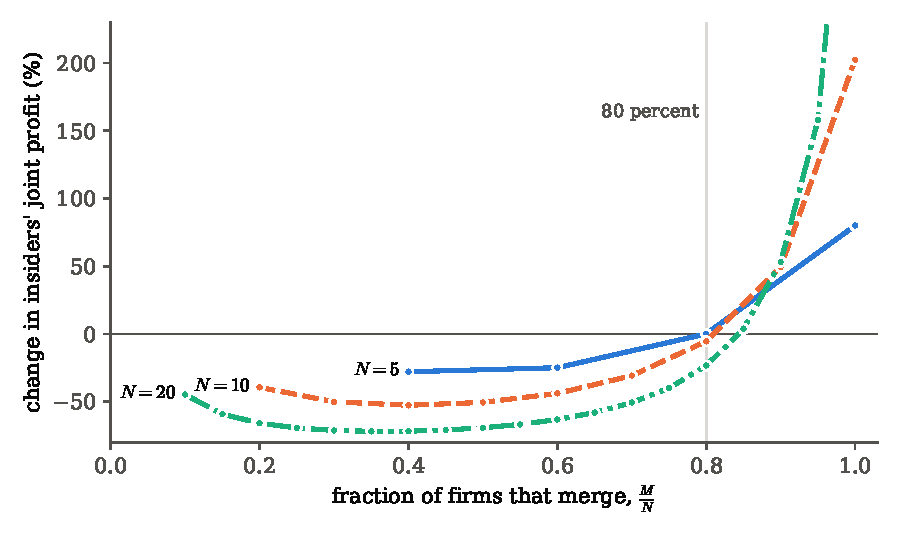
\includegraphics[width=0.8\textwidth]{figures/ch11/ssr_paradox.pdf}
\caption{The merger paradox. Percentage change in the joint profit of $M$ merging firms in a linear Cournot
market with $N$ symmetric firms and no cost savings, $100\big[\frac{(N + 1)^2}{M(N - M + 2)^2} - 1\big]$, against
$\frac{M}{N}$. Points above zero are profitable mergers. Curves are clipped at 230 percent.}
\label{fig:11-ssr}
\end{figure}

The reason is the response of the outsiders. In Cournot competition, quantities are strategic substitutes. When
the merged firm cuts its output, the outsiders expand theirs and capture much of the benefit of the higher price.
Moreover, a merger in this model is equivalent to $M - 1$ firms shutting down. The merged firm is no larger and no
more efficient than any other firm, so it ends up with a share of only $\frac{1}{N - M + 1}$
\citep[p.~4]{FarrellShapiro1988}. The paradox is that we observe many horizontal mergers.

Three features of the model drive the result, and relaxing any of them can overturn it. First, the merging firms
bring no assets. \citet{PerryPorter1985} let each firm own capital that lowers its marginal cost, so the merged
firm has the combined capital and is larger than its rivals. Mergers can then be profitable, and
\cref{sec:11-fs} develops this idea in general. Second, the model has no investment. \citet[Remark
3]{Pesendorfer2003} considers firms that hold capacity, with linear demand $P = a - bQ$, constant marginal cost
$c$, a linear cost $r$ per unit of new capacity, and initial capacities at Cournot levels. He also normalizes the
discount and depreciation factors. He shows that a merger
without cost savings is profitable whenever $n + 1 > \frac{a - c}{r}$. Building capacity is costly while scrapping
it is not, and this asymmetry favors the merged firm. The Salant-Switzer-Reynolds result is the limit as $r \to 0$
\citep[p.~7, n.~6]{Pesendorfer2003}. \Cref{sec:11-beyond} returns to this model. Third, quantities are strategic
substitutes. With price competition and differentiated products, rivals raise their prices after a merger, and
the merger is profitable (\cref{sec:11-upp}).

\subsection{Farrell and Shapiro (1990): mergers as transfers of capital}\label{sec:11-fs}

\casehead{The question}
\citet{FarrellShapiro1990} ask when a horizontal merger raises the price, when it raises welfare, and what a
regulator can infer from the fact that the merging firms want to merge. Their answer rests on three ideas. A merger
is a transfer of industry-specific capital from one firm to another. The welfare effect of a merger can be split
into the change in the merging firms' profits, which they internalize, and an \emph{external effect} on consumers
and rivals. The external effect depends only on observable market data, while the private effect may include
synergies that only the firms know. A regulator should therefore approve any merger that is proposed and has a
positive external effect, because private profitability then guarantees a welfare gain. We follow the 1988
working-paper version \citep{FarrellShapiro1988}, whose numbering of equations and propositions differs from the
published article. The result on the cost savings needed to lower the price belongs to the published article
\citep{FarrellShapiro1990} and is not in the working paper. We state it as \citet[pp.~216--217 and
229]{AskerNocke2021} report it, and we prove it in full.

\subsubsection{The model}

There are $N$ firms producing a homogeneous good, and their number is fixed by barriers to entry. A competitive
fringe can be absorbed into the demand curve, which is then a residual demand. We write $q_i$ for firm $i$'s
output, $Q = \sum_i q_i$ for industry output, $P(Q)$ for inverse demand and $s_i = \frac{q_i}{Q}$ for market
shares (Farrell and Shapiro write $x_i$, $X$ and $p(X)$).

\begin{assumption}[Cournot oligopoly with capital]\label{ass:11-fs}
\leavevmode
\begin{enumerate}[label=(\roman*)]
  \item Inverse demand $P(Q)$ is twice differentiable with $P'(Q) < 0$.
  \item Firm $i$ owns capital $k_i$ and has a twice differentiable cost function $C^i(q_i, k_i)$. More capital
  lowers marginal cost, $C^i_{qk} < 0$, where subscripts denote partial derivatives.
  \item Given the capital vector $k = (k_1, \dots, k_N)$, firms choose outputs simultaneously (Cournot). The
  equilibrium is unique and interior.
  \item Reaction functions slope down and the equilibrium is stable. Formally, at the equilibrium,
  $P' + q_i P'' < 0$ and $C^i_{qq} - P' > 0$ for every firm.
\end{enumerate}
\end{assumption}

Firms may have different technologies, and $C^i$ may then embody firm-specific assets that cannot be transferred.
Capital is industry specific and fixed in the short run, while outputs adjust quickly. Firm $i$ maximizes
$\pi_i = P(Q)\,q_i - C^i(q_i, k_i)$, with first-order condition
\begin{equation}\label{eq:11-fs-foc}
P(Q) + q_i P'(Q) - C^i_q(q_i, k_i) = 0, \qquad i = 1, \dots, N.
\end{equation}
The condition implies $P - C^i_q = -q_i P'$, so each firm's margin over marginal cost is proportional to its
output. Comparing two firms, $q_i > q_j$ if and only if $C^i_q < C^j_q$. In a Cournot equilibrium, \emph{larger
firms have lower marginal costs}. Whenever firms produce different quantities, marginal costs differ, so total
cost is not minimized for the industry's output. Shifting output toward large firms would lower it.

Welfare is consumers' gross benefit minus production costs,
\begin{equation*}
W = \int_0^Q P(z)\,\dd z - \sum_{i=1}^{N} C^i(q_i, k_i).
\end{equation*}

\subsubsection{Profit and welfare effects of a change in capital}

Consider a small change $\dd k = (\dd k_1, \dots, \dd k_N)$ in the allocation of capital, and the induced changes
$\dd q_i$ in outputs. Differentiating $\pi_i$,
\begin{equation}\label{eq:11-fs-dpi}
\dd\pi_i = (P - C^i_q)\,\dd q_i + q_i P'\,\dd Q - C^i_k\,\dd k_i .
\end{equation}
A firm gains from extra output in proportion to its margin, gains from a price increase in proportion to its
output, and saves costs through its own capital. Differentiating $W$ and using $\frac{\dd}{\dd Q}\int_0^Q P = P$,
\begin{equation}\label{eq:11-fs-dw}
\dd W = \sum_{i=1}^{N} (P - C^i_q)\,\dd q_i - \sum_{i=1}^{N} C^i_k\,\dd k_i .
\end{equation}
The first sum values each change in output at the gap between price and marginal cost. The second is the direct
effect of capital on costs at given outputs. Equations \eqref{eq:11-fs-dpi} and \eqref{eq:11-fs-dw} hold for any
theory of oligopoly. Under Cournot competition, $P - C^i_q = -q_i P'$, and \eqref{eq:11-fs-dw} becomes
\begin{equation}\label{eq:11-fs-dw-cournot}
\dd W = -P'\sum_{i=1}^{N} q_i\,\dd q_i - \sum_{i=1}^{N} C^i_k\,\dd k_i .
\end{equation}

\begin{lemma}[Welfare and the Herfindahl index]\label{lem:11-fs-hhi}
Under \cref{ass:11-fs},
\begin{equation}\label{eq:11-fs-dw-hhi}
\dd W = -P'\Big(\HHI\,Q\,\dd Q + \frac{1}{2}Q^2\,\dd\HHI\Big) - \sum_{i=1}^{N} C^i_k\,\dd k_i .
\end{equation}
\end{lemma}

\begin{proof}
Since $\HHI = \sum_i \big(\frac{q_i}{Q}\big)^2$, we have $Q^2\HHI = \sum_i q_i^2$. Differentiating both sides,
\begin{equation*}
2\sum_i q_i\,\dd q_i = \dd\big(Q^2\HHI\big) = 2\HHI\,Q\,\dd Q + Q^2\,\dd\HHI .
\end{equation*}
Dividing by two and substituting into \eqref{eq:11-fs-dw-cournot} gives \eqref{eq:11-fs-dw-hhi}.
\end{proof}

\Cref{lem:11-fs-hhi} splits a welfare change into three parts: a change in industry output, a change in its
distribution, and the direct effect on costs. More output raises welfare because price exceeds marginal cost.
More surprisingly, for a given change in output, a larger increase in the Herfindahl index raises welfare more,
since $-P' > 0$. Large firms have the lowest marginal costs, so shifting output toward them saves resources. Any
analysis that treats increases in concentration as bad per se is therefore misleading under Cournot competition
\citep[p.~8]{FarrellShapiro1988}.

\subsubsection{Comparative statics}

\begin{lemma}[Output responses]\label{lem:11-fs-statics}
Under \cref{ass:11-fs}, define for each firm
\begin{equation}\label{eq:11-fs-lambda}
\lambda_i = \frac{-P' - q_i P''}{C^i_{qq} - P'} > 0,
\qquad
\chi_i = \frac{-C^i_{qk}}{C^i_{qq} - P'} > 0,
\qquad
\Lambda = \sum_{i=1}^{N}\lambda_i .
\end{equation}
A small change $\dd k$ changes outputs by
\begin{equation}\label{eq:11-fs-dq}
\dd q_i = -\lambda_i\,\dd Q + \chi_i\,\dd k_i,
\qquad
\dd Q = \frac{1}{1 + \Lambda}\sum_{i=1}^{N}\chi_i\,\dd k_i .
\end{equation}
\end{lemma}

\begin{proof}
Totally differentiate the first-order condition \eqref{eq:11-fs-foc}, holding the equilibrium:
\begin{equation*}
\big(P' + q_i P''\big)\,\dd Q + P'\,\dd q_i - C^i_{qq}\,\dd q_i - C^i_{qk}\,\dd k_i = 0 .
\end{equation*}
Collect the terms in $\dd q_i$:
\begin{equation*}
\big(C^i_{qq} - P'\big)\,\dd q_i = \big(P' + q_i P''\big)\,\dd Q - C^i_{qk}\,\dd k_i .
\end{equation*}
Dividing by $C^i_{qq} - P' > 0$ gives the first part of \eqref{eq:11-fs-dq}. Signs follow from part (iv) of
\cref{ass:11-fs} and from $C^i_{qk} < 0$. Summing over $i$,
\begin{equation*}
\dd Q = -\Lambda\,\dd Q + \sum_i \chi_i\,\dd k_i ,
\end{equation*}
and solving for $\dd Q$ gives the second part.
\end{proof}

The coefficient $\chi_i$ is the \emph{direct effect} of firm $i$'s capital on its output at a given industry
output (Farrell and Shapiro call it $\delta_i$). The coefficient $\lambda_i$ measures how firm $i$ responds to a
change in industry output, and hence to the price. A firm whose capital does not change adjusts its output by
$\dd q_i = -\lambda_i\,\dd Q$. Its response to the combined output of the others, $Q_{-i}$, follows from
$\dd Q = \dd q_i + \dd Q_{-i}$ and is $\frac{\dd q_i}{\dd Q_{-i}} = -\frac{\lambda_i}{1 + \lambda_i}$. Two special
cases recur. With constant marginal cost, $C^i_{qq} = 0$ and
\begin{equation}\label{eq:11-fs-lambda-const}
\lambda_i = \frac{-P' - q_i P''}{-P'} = 1 + \frac{q_i P''}{P'} = 1 - s_i\,\mathcal{E},
\qquad
\mathcal{E} = -\frac{Q P''(Q)}{P'(Q)},
\end{equation}
where $\mathcal{E}$ is the elasticity of the slope of inverse demand (Farrell and Shapiro write $E$). With linear
demand $P = a - Q$ and the cost function $C(q, k) = \frac{q^2}{2k}$, we have $C_{qq} = \frac{1}{k}$ and
$P' = -1$, so $\lambda_i = \frac{1}{1 + \frac{1}{k_i}} = \frac{k_i}{1 + k_i}$.

\begin{example}[Two technologies]\label{ex:11-fs-tech}
\emph{Physical capital.} Let $P(Q) = a - Q$ and $C(q, k) = \frac{q^2}{2k}$ for all firms. This technology has
constant returns to scale and corresponds to the production function $q = \sqrt{kv}$ with a variable input $v$.
Firm $i$'s first-order condition is $a - Q - q_i - \frac{q_i}{k_i} = 0$. Define the \emph{adjusted capital}
$\tilde k_i = \frac{k_i}{1 + k_i}$. The condition becomes
\begin{equation*}
q_i\Big(1 + \frac{1}{k_i}\Big) = a - Q
\quad\Longrightarrow\quad
q_i = (a - Q)\,\tilde k_i = P\,\tilde k_i .
\end{equation*}
Summing over firms, $Q = (a - Q)\tilde K$ with $\tilde K = \sum_i \tilde k_i$, so
\begin{equation*}
Q = \frac{a\tilde K}{1 + \tilde K}, \qquad P = \frac{a}{1 + \tilde K}, \qquad
C^i_q = \frac{q_i}{k_i} = \frac{P}{1 + k_i} .
\end{equation*}
Firms with more capital produce more and have lower marginal costs. Here $\lambda_i = \tilde k_i = \frac{q_i}{P}$,
and the direct effect is
\begin{equation*}
\chi_i = \frac{\frac{q_i}{k_i^2}}{\frac{1}{k_i} + 1} = \frac{q_i}{k_i(1 + k_i)} = \frac{P}{(1 + k_i)^2} .
\end{equation*}
\emph{Know-how.} Let unit cost depend on capital but not on output, $C(q, k) = q\,\phi(k)$ with $\phi' < 0$. This
fits patents, know-how and managerial talent, which can be applied to any scale of output. The first-order
conditions are $P + q_i P' = \phi(k_i)$, and summing them gives
\begin{equation}\label{eq:11-fs-knowhow}
N P(Q) + Q P'(Q) = \sum_{i=1}^{N}\phi(k_i),
\end{equation}
so industry output depends on capital only through the sum of marginal costs.
\end{example}

\subsubsection{Investment by one firm}

Before turning to mergers, consider investment, $\dd k = (\dd k_1, 0, \dots, 0)$. By \cref{lem:11-fs-statics},
\begin{equation*}
\frac{\dd Q}{\dd k_1} = \frac{\chi_1}{1 + \Lambda}, \qquad
\frac{\dd q_i}{\dd k_1} = -\frac{\lambda_i\chi_1}{1 + \Lambda}\ (i \ne 1), \qquad
\frac{\dd q_1}{\dd k_1} = \chi_1\Big(1 - \frac{\lambda_1}{1 + \Lambda}\Big).
\end{equation*}
The investing firm expands, its rivals contract, and industry output rises. Subtracting \eqref{eq:11-fs-dw} from
\eqref{eq:11-fs-dpi} for $i = 1$, the private and social returns differ by
\begin{equation}\label{eq:11-fs-invest-wedge0}
\dd\pi_1 - \dd W = q_1 P'\,\dd Q - \sum_{i \ne 1}(P - C^i_q)\,\dd q_i .
\end{equation}
The first term is a private loss that is a transfer to consumers: the investor's price falls on its own sales. The
second is a social cost the investor ignores: rivals, whose price exceeds marginal cost, cut their output. Using
$P - C^i_q = -q_i P'$ and $\dd q_i = -\lambda_i\,\dd Q$ for $i \ne 1$,
\begin{equation}\label{eq:11-fs-invest-wedge}
\frac{\dd\pi_1}{\dd k_1} - \frac{\dd W}{\dd k_1}
= -P'\,\frac{\dd Q}{\dd k_1}\Big(\sum_{i \ne 1}\lambda_i q_i - q_1\Big).
\end{equation}

\begin{proposition}[Investment incentives]\label{prop:11-fs-invest}
Under \cref{ass:11-fs}, firm 1 has an excessive incentive to invest, $\frac{\dd\pi_1}{\dd k_1} >
\frac{\dd W}{\dd k_1}$, if and only if
\begin{equation}\label{eq:11-fs-invest}
s_1 < \sum_{i \ne 1}\lambda_i s_i .
\end{equation}
With linear demand and the costs $\frac{q^2}{2k}$, the condition is $s_1 < \frac{1}{\varepsilon}\sum_{i \ne 1}s_i^2$,
where $\varepsilon = -\frac{P}{QP'}$. With constant marginal costs, it is
$s_1 < \frac{1}{2} - \frac{\mathcal{E}}{2}\sum_{i \ne 1}s_i^2$.
\end{proposition}

\begin{proof}
In \eqref{eq:11-fs-invest-wedge}, $-P' > 0$ and $\frac{\dd Q}{\dd k_1} > 0$, so the wedge is positive if and only
if $\sum_{i \ne 1}\lambda_i q_i > q_1$. Dividing by $Q$ gives \eqref{eq:11-fs-invest}. In the quadratic case,
$\lambda_i = \frac{q_i}{P}$, so $\sum_{i \ne 1}\lambda_i s_i = \frac{Q}{P}\sum_{i \ne 1}s_i^2$, and
$\frac{Q}{P} = \frac{1}{\varepsilon}$ because $P' = -1$. With constant marginal costs,
$\sum_{i \ne 1}(1 - s_i\mathcal{E})s_i = 1 - s_1 - \mathcal{E}\sum_{i \ne 1}s_i^2$, and the inequality
$s_1 < 1 - s_1 - \mathcal{E}\sum_{i \ne 1}s_i^2$ rearranges to the stated form.
\end{proof}

Small firms invest too much. Their investment lowers the price and helps consumers, but it steals valuable
business from larger rivals with high margins, and the second effect dominates \citep[pp.~10--11]{FarrellShapiro1988}.
If $\lambda_i$ rises with firm size, as in the quadratic case, large efficient firms invest too little.

\subsubsection{Small capital transfers and the price}

A merger moves capital from one firm to another. Consider a small transfer from firm 2 to firm 1,
$\dd k_1 = \dd k = -\dd k_2 > 0$, with $k_1 > k_2$, so that the transfer increases the concentration of capital.
A complete merger of the two firms is the accumulation of such transfers, from $(k_1, k_2)$ to $(k_1 + k_2, 0)$.
Divestitures are the reverse.

\begin{proposition}[Price effect of a transfer]\label{prop:11-fs-price}
Under \cref{ass:11-fs}, a small transfer of capital from firm 2 to firm 1 changes industry output by
\begin{equation}\label{eq:11-fs-dqdk}
\frac{\dd Q}{\dd k} = \frac{\chi_1 - \chi_2}{1 + \Lambda}.
\end{equation}
It reduces output and raises the price if and only if $\chi_1 < \chi_2$, that is, if and only if the direct
output effect of capital is smaller at the acquiring firm.
\end{proposition}

\begin{proof}
Substitute $\dd k_1 = \dd k$, $\dd k_2 = -\dd k$ and $\dd k_i = 0$ for $i \ge 3$ into \eqref{eq:11-fs-dq}. Since
$1 + \Lambda > 0$, the sign of $\dd Q$ is the sign of $\chi_1 - \chi_2$.
\end{proof}

In the physical-capital example, $\chi_i = \frac{P}{(1 + k_i)^2}$ falls with $k_i$, so every
concentration-increasing transfer raises the price. The same follows from the closed form $P = \frac{a}{1 + \tilde
K}$. Adjusted capital $\tilde k(k) = \frac{k}{1 + k}$ is strictly concave with $\tilde k(0) = 0$, so moving capital
from the smaller to the larger firm lowers $\tilde k_1 + \tilde k_2$, and a complete merger gives
$\tilde k(k_1 + k_2) < \tilde k(k_1) + \tilde k(k_2)$. In the know-how example, \eqref{eq:11-fs-knowhow} shows
that output falls if and only if the transfer raises $\sum_i\phi(k_i)$, and the transfer changes this sum by
$\big(\phi'(k_1) - \phi'(k_2)\big)\dd k$. With $k_1 > k_2$, the price rises if and only if $\phi'' > 0$. A merger of
know-how raises the price when units of know-how are substitutes, which lower unit cost at a diminishing rate. It
lowers the price when they are complements.

\Cref{prop:11-fs-price} needs the $\chi_i$, which are hard to measure. A condition on the technology alone is more
useful.

\begin{proposition}[A sufficient condition, \citealp{FarrellShapiro1988}]\label{prop:11-fs-convex}
Suppose that, in addition to \cref{ass:11-fs}, all firms share the cost function $C(q, k)$ and the marginal cost
$C_q$ is jointly convex in $(q, k)$. Then every concentration-increasing transfer, small or large, weakly reduces
output and weakly raises the price, as long as the selling firm remains active. The effects are strict when the Hessian
of $C_q$ is positive definite.
\end{proposition}

\begin{proof}
Fix industry output $Q$, and let $\tilde q(Q, k)$ be the output of a firm with capital $k$ that satisfies the
first-order condition, $P(Q) + \tilde q P'(Q) = C_q(\tilde q, k)$. Because the technology is common, firm $i$'s output in
equilibrium is $\tilde q(Q, k_i)$ and its direct effect is $\chi_i = \tilde q_k(Q, k_i)$. To see this, differentiate the
condition in $k$ at fixed $Q$:
\begin{equation*}
P'\,\tilde q_k = C_{qq}\,\tilde q_k + C_{qk}
\quad\Longrightarrow\quad
\tilde q_k = \frac{-C_{qk}}{C_{qq} - P'} = \chi .
\end{equation*}
Differentiating once more in $k$,
\begin{equation*}
P'\,\tilde q_{kk} = C_{qqq}\,\tilde q_k^2 + 2C_{qqk}\,\tilde q_k + C_{qkk} + C_{qq}\,\tilde q_{kk},
\end{equation*}
so
\begin{equation*}
\tilde q_{kk} = -\frac{C_{qqq}\,\tilde q_k^2 + 2C_{qqk}\,\tilde q_k + C_{qkk}}{C_{qq} - P'} .
\end{equation*}
The numerator is $\gamma^\top H\gamma$ with $\gamma = (\tilde q_k, 1)^\top$ and $H$ the Hessian of $C_q$. Joint
convexity makes it nonnegative, so $\tilde q_{kk} \le 0$ and $\chi = \tilde q_k$ is nonincreasing in $k$ across firms.
Hence $k_1 > k_2$ implies $\chi_1 \le \chi_2$, and \cref{prop:11-fs-price} applies. A positive definite Hessian
makes the numerator positive, because $\gamma \ne 0$, and then $\chi_1 < \chi_2$. A large transfer is a sequence of small transfers, each from the smaller to the larger firm,
so output falls along the whole path.
\end{proof}

Farrell and Shapiro add that the condition is sufficient but not necessary. The physical-capital technology
violates it, since its marginal cost $\frac{q}{k}$ is not jointly convex, yet every merger raises the price there.
The know-how technology satisfies it exactly when $\phi'' \ge 0$, since $C_q = \phi(k)$. Its Hessian is
singular, yet the numerator in the proof equals $\phi''(k)$, so the price rises strictly when $\phi'' > 0$. Under the conditions of
\cref{prop:11-fs-price,prop:11-fs-convex}, a merger harms consumers. Because rivals' profits rise exactly when the
price rises, the same conditions tell us when rivals gain \citep[p.~15]{FarrellShapiro1988}.

\subsubsection{Discrete mergers and the synergies needed to lower the price}

A merger can also reorganize production or create synergies that a reallocation of existing capital cannot
capture. To study such mergers, we replace capital by constant marginal costs. Firm $i$ has marginal cost $c_i$.
Firms 1 and 2 merge, and the merged firm has marginal cost $c_M$, which summarizes its post-merger technology. A
merger with no synergies can at best produce everything at the lower of the two costs, $c_M = \min\{c_1, c_2\}$.
We write $P^0 = P(Q^0)$ for the pre-merger price.

\begin{proposition}[Synergies needed to lower the price, \citealp{FarrellShapiro1990}]\label{prop:11-synergy}
Suppose firms have constant marginal costs, $P'(Q) + qP''(Q) < 0$ for all $0 \le q \le Q$, and all firms are active
before and after the merger. The merger of firms 1 and 2 lowers the equilibrium price if and only if
\begin{equation}\label{eq:11-synergy}
c_M < \hat c \equiv c_1 + c_2 - P^0,
\quad\text{equivalently}\quad
P^0 - c_M > (P^0 - c_1) + (P^0 - c_2).
\end{equation}
It leaves the price unchanged if $c_M = \hat c$ and raises it if $c_M > \hat c$.
\end{proposition}

\begin{proof}
Summing the first-order conditions $P + q_i P' = c_i$ over the $n$ active firms gives the aggregate condition
\begin{equation*}
\Gamma_n(Q) \equiv nP(Q) + QP'(Q) = \sum_{i \text{ active}} c_i .
\end{equation*}
Its slope is $\Gamma_n'(Q) = P' + \sum_{i}\big(P' + q_i P''\big) < 0$, so $\Gamma_n$ is strictly decreasing and
the equilibrium output is the unique solution. Only the number of firms and the sum of their marginal costs
matter for $Q$. Before the merger,
\begin{equation*}
N P^0 + Q^0 P'(Q^0) = c_1 + c_2 + \sum_{i \ge 3} c_i .
\end{equation*}
After the merger there are $N - 1$ firms, and the post-merger output $Q^1$ solves
$\Gamma_{N-1}(Q^1) = c_M + \sum_{i \ge 3}c_i$. Evaluate $\Gamma_{N-1}$ at the pre-merger output and use the
pre-merger condition:
\begin{equation*}
\Gamma_{N-1}(Q^0) = N P^0 + Q^0 P'(Q^0) - P^0 = c_1 + c_2 - P^0 + \sum_{i \ge 3}c_i .
\end{equation*}
Since $\Gamma_{N-1}$ is decreasing, $Q^1 > Q^0$ if and only if
$\Gamma_{N-1}(Q^1) < \Gamma_{N-1}(Q^0)$, that is, if and only if
\begin{equation*}
c_M + \sum_{i \ge 3}c_i < c_1 + c_2 - P^0 + \sum_{i \ge 3}c_i
\quad\Longleftrightarrow\quad
c_M < c_1 + c_2 - P^0 .
\end{equation*}
A higher output means a lower price. The cases of equality and of the reverse inequality follow the same way.
\end{proof}

\begin{corollary}[No synergies, higher price]\label{prop:11-nosynergy}
Under the conditions of \cref{prop:11-synergy}, the price-neutral cost satisfies $\hat c < \min\{c_1, c_2\}$.
Any merger with $c_M \ge \min\{c_1, c_2\}$, including every merger that only rationalizes production, raises the
price.
\end{corollary}

\begin{proof}
Firm 2 is active before the merger, so $P^0 - c_2 = -q_2 P'(Q^0) > 0$. Hence
$\hat c = c_1 - (P^0 - c_2) < c_1$. By the same argument with the roles reversed, $\hat c < c_2$. If
$c_M \ge \min\{c_1, c_2\}$, then $c_M > \hat c$, and \cref{prop:11-synergy} applies.
\end{proof}

The required synergy is large. Let firm 1 be the more efficient partner. The merged firm's cost must fall below
$c_1$ by firm 2's entire margin, $c_1 - \hat c = P^0 - c_2$. As a fraction of the price, the reduction equals firm
2's Lerner index, $\frac{c_1 - \hat c}{P^0} = \frac{s_2}{\varepsilon}$. As a fraction of firm 1's cost it is
$\frac{L_2}{1 - L_1}$, where $L_i = \frac{P^0 - c_i}{P^0}$. Two firms with 20 percent shares each, facing a market
elasticity of one, have $L_1 = L_2 = 0.2$. For their merger not to raise the price, marginal cost must fall by
$\frac{0.2}{0.8} = 25$ percent.

The required reduction can also be written with the naive change in concentration. Let $s_I = s_1 + s_2$ and let
$\bar c = \frac{s_1 c_1 + s_2 c_2}{s_I}$ be the partners' share-weighted marginal cost. The first-order conditions
give $P^0 - c_i = \frac{s_i P^0}{\varepsilon}$, so
\begin{align*}
P^0 - \bar c &= \frac{s_1(P^0 - c_1) + s_2(P^0 - c_2)}{s_I} = \frac{s_1^2 + s_2^2}{s_I}\cdot\frac{P^0}{\varepsilon},\\
P^0 - \hat c &= (P^0 - c_1) + (P^0 - c_2) = s_I\,\frac{P^0}{\varepsilon}.
\end{align*}
Subtracting the first line from the second,
\begin{equation}\label{eq:11-required-dhhi}
\frac{\bar c - \hat c}{P^0} = \frac{1}{\varepsilon}\Big(s_I - \frac{s_1^2 + s_2^2}{s_I}\Big)
= \frac{(s_1 + s_2)^2 - s_1^2 - s_2^2}{\varepsilon\, s_I} = \frac{2 s_1 s_2}{\varepsilon\, s_I} .
\end{equation}
The numerator is the naive $\Delta\HHI$ of \eqref{eq:11-dhhi}. The outsiders' shares do not enter, so for given
shares of the merging firms the required efficiency does not depend on the level of the index. This parallels the
finding of \citet{NockeWhinston2020}, reported in \cref{sec:11-hhi}, that required efficiencies track the change in
concentration and not its level. In the example above,
$\frac{2 \times 0.2 \times 0.2}{0.4} = 0.2$ of the price, which is 25 percent of $\bar c = 0.8 P^0$.

\Cref{prop:11-synergy} is the condition that \citet[Lemma 1 and eq.~(5)]{NockeWhinston2013} use to define a
\emph{CS-neutral merger}, one that leaves consumer surplus unchanged. In their notation, with acquirer 0 and
target $k$, the condition is $\bar c_k = c_k - \big[P(Q^0) - c_0\big]$, the same as \eqref{eq:11-synergy}. They also
note that such a merger is profitable. The argument is short.

\begin{corollary}[A price-neutral merger is profitable]\label{cor:11-neutral-profit}
Under the conditions of \cref{prop:11-synergy}, let $c_M = \hat c$. The merger leaves the price and every
outsider's output unchanged and gives the merged firm the output $q_1 + q_2$. It raises the joint profit of the
merging firms by $(P^0 - c_1)q_2 + (P^0 - c_2)q_1 > 0$.
\end{corollary}

\begin{proof}
With $c_M = \hat c$, \cref{prop:11-synergy} gives $Q^1 = Q^0$, so the price and its slope are unchanged. Each
outsider's first-order condition $P + q_i P' = c_i$ then gives the same $q_i$. The merged firm produces the rest,
$Q^0 - \sum_{i \ge 3}q_i = q_1 + q_2$. Its profit is
\begin{align*}
(P^0 - \hat c)(q_1 + q_2)
&= \big[(P^0 - c_1) + (P^0 - c_2)\big](q_1 + q_2) \\
&= \underbrace{(P^0 - c_1)q_1 + (P^0 - c_2)q_2}_{\pi_1 + \pi_2} + (P^0 - c_1)q_2 + (P^0 - c_2)q_1 .
\end{align*}
Both extra terms are positive because both firms were active.
\end{proof}

\Cref{fig:11-synergy} illustrates these results. Demand is $P = 10 - Q$ and three firms have costs
$(c_1, c_2, c_3) = (2, 3, 3)$, so $P^0 = 4.5$ and outputs are $(2.5, 1.5, 1.5)$. If firms 1 and 2 merge, the
post-merger price is $\frac{13 + c_M}{3}$. The price-neutral cost is $\hat c = 2 + 3 - 4.5 = 0.5$, well below
$c_1 = 2$. Rationalization alone, $c_M = 2$, raises the price to 5. This merger is still profitable, because the
merged firm earns 9 against the 8.5 the two firms earned before. It lowers total surplus by 0.375, as consumers
lose 2.625 while the outsider gains 1.75. Every cost between 0.5 and about 2.13 makes the merger both profitable
and price-increasing. Total surplus rises only for costs below about 1.91.

\begin{figure}[htbp]
\centering
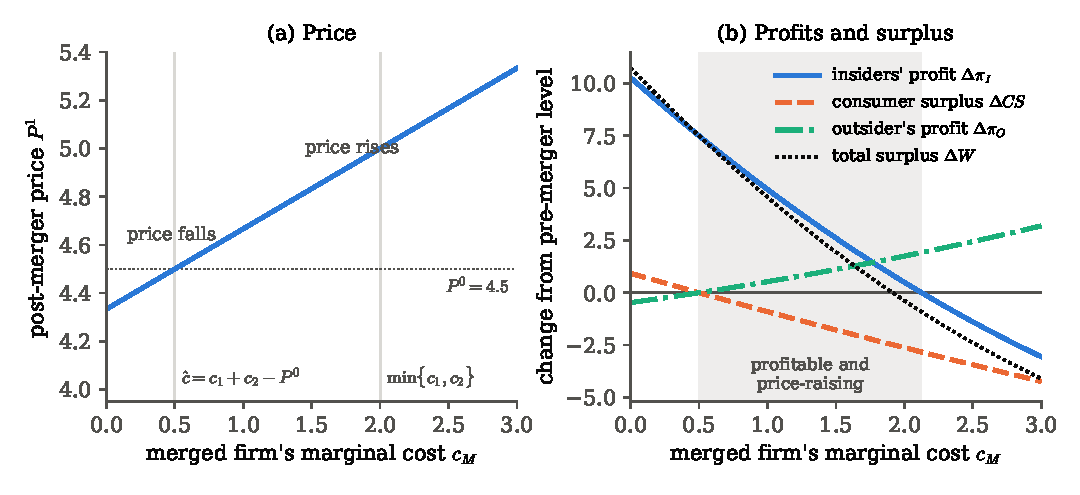
\includegraphics[width=\textwidth]{figures/ch11/cournot_synergy.pdf}
\caption{A Cournot merger with constant marginal costs. Demand $P = 10 - Q$, costs $(c_1, c_2, c_3) = (2, 3, 3)$,
and firms 1 and 2 merge with marginal cost $c_M$. Panel (a) shows the post-merger price, with the price-neutral cost
$\hat c = 0.5$ and the rationalization cost $\min\{c_1, c_2\} = 2$. Panel (b) shows the changes in the insiders'
joint profit, consumer surplus, the outsider's profit and total surplus. The shaded band, $0.5 < c_M < 2.13$, contains
the mergers that are profitable and raise the price. Total surplus falls for $c_M > 1.91$.}
\label{fig:11-synergy}
\end{figure}

\subsubsection{General costs, many partners and aggregate surplus}

\Cref{prop:11-synergy} assumes constant marginal costs and two partners. \citet[p.~229, eq.~(6)]{AskerNocke2021}
state the condition of \citet{FarrellShapiro1990} for any cost functions and any number of partners. We hold capital
fixed and write $C_i(q_i)$ for firm $i$'s cost function. A set $\mathcal{M}$ of at least two firms merges into a firm
with cost function $C_{\mathcal{M}}(q)$, and $q_{\mathcal{M}}^0 = \sum_{i \in \mathcal{M}} q_i^0$ is the partners'
combined pre-merger output.

\begin{proposition}[The synergy condition with general costs, \citealp{FarrellShapiro1990}]\label{prop:11-synergy-gen}
Let \cref{ass:11-fs} hold with capital fixed, let $C''_{\mathcal{M}} - P' > 0$, and let all firms be active before
and after the merger. The merger weakly raises industry output, and so does not lower consumer surplus, if and only
if
\begin{equation}\label{eq:11-an6}
P(Q^0) - C'_{\mathcal{M}}\big(q_{\mathcal{M}}^0\big) \;\ge\; \sum_{i \in \mathcal{M}}\big[P(Q^0) - C'_i(q_i^0)\big].
\end{equation}
It weakly lowers industry output if and only if the reverse weak inequality holds.
\end{proposition}

\begin{proof}
For a firm with cost function $C$, define its \emph{fitting-in output} $r(Q)$ as the solution in $q$ of $P(Q) +
qP'(Q) = C'(q)$. It is the output at which the firm's first-order condition holds when industry output is $Q$. The
left side minus the right side falls in $q$ at rate $P' - C'' < 0$, so $r(Q)$ is unique. Differentiating the
condition in $Q$,
\begin{equation*}
P' + r'P' + rP'' = C''r'
\quad\Longrightarrow\quad
r'(Q) = \frac{P' + rP''}{C'' - P'} = -\lambda ,
\end{equation*}
with $\lambda > 0$ the response coefficient of \cref{lem:11-fs-statics}. An equilibrium is an industry output at
which the fitting-in outputs add up to $Q$. After the merger, let
\begin{equation*}
\Phi(Q) = \sum_{i \notin \mathcal{M}} r_i(Q) + r_{\mathcal{M}}(Q) - Q .
\end{equation*}
It is strictly decreasing, with slope $-\sum_{i \notin \mathcal{M}}\lambda_i - \lambda_{\mathcal{M}} - 1 < 0$, so
the post-merger output $Q^1$ is its unique zero, and $Q^1 \ge Q^0$ if and only if $\Phi(Q^0) \ge 0$. At $Q^0$ each
outsider's fitting-in output is its pre-merger output, $r_i(Q^0) = q_i^0$. Hence
\begin{equation*}
\Phi(Q^0) = \sum_{i \notin \mathcal{M}} q_i^0 + r_{\mathcal{M}}(Q^0) - Q^0 = r_{\mathcal{M}}(Q^0) - q_{\mathcal{M}}^0 .
\end{equation*}
The merged firm's marginal profit at fixed $Q^0$, $P(Q^0) + qP'(Q^0) - C'_{\mathcal{M}}(q)$, falls in $q$ and is
zero at $r_{\mathcal{M}}(Q^0)$. So $r_{\mathcal{M}}(Q^0) \ge q_{\mathcal{M}}^0$ if and only if the marginal profit
is nonnegative at $q_{\mathcal{M}}^0$:
\begin{equation*}
P(Q^0) + q_{\mathcal{M}}^0P'(Q^0) - C'_{\mathcal{M}}\big(q_{\mathcal{M}}^0\big) \ge 0 .
\end{equation*}
The partners' pre-merger first-order conditions give $q_i^0P'(Q^0) = -\big[P(Q^0) - C'_i(q_i^0)\big]$. Summing over
$i \in \mathcal{M}$,
\begin{equation*}
q_{\mathcal{M}}^0P'(Q^0) = -\sum_{i \in \mathcal{M}}\big[P(Q^0) - C'_i(q_i^0)\big] .
\end{equation*}
Substituting into the marginal profit gives \eqref{eq:11-an6}. The reverse case follows from the same steps with
the inequalities reversed.
\end{proof}

With constant marginal costs and two partners, \eqref{eq:11-an6} is \eqref{eq:11-synergy}. Every term on the right of
\eqref{eq:11-an6} is positive, because each partner was active. The right side therefore exceeds each single term
$P(Q^0) - C'_j(q_j^0)$. The condition thus requires the merged firm's marginal cost at the combined output to lie
below the pre-merger marginal cost of every partner, $C'_{\mathcal{M}}(q_{\mathcal{M}}^0) < \min_{i \in
\mathcal{M}}C'_i(q_i^0)$ \citep[p.~229]{AskerNocke2021}.

A merger can raise productive efficiency even without synergies, in the sense of \citet{FarrellShapiro1990}. Say
the merger creates \emph{no synergies} when the merged firm can do no better than allocate output among the
partners' existing technologies,
\begin{equation}\label{eq:11-nosynergy-cost}
C_{\mathcal{M}}(q) = \min\Big\{\sum_{i \in \mathcal{M}}C_i(q_i) : \sum_{i \in \mathcal{M}}q_i = q,\ q_i \ge 0\Big\}.
\end{equation}
By the pre-merger first-order conditions, $P - C'_i(q_i^0) = -q_i^0P'$, so the smaller partner has the higher
marginal cost. Shifting output from it to the larger partner lowers the cost of producing $q_{\mathcal{M}}^0$. The
next result shows that such output shifting is not enough.

\begin{corollary}[Rationalization is not enough]\label{cor:11-rationalize}
Under the conditions of \cref{prop:11-synergy-gen}, suppose every $C_i$ is convex and the merger creates no
synergies, as in \eqref{eq:11-nosynergy-cost}. Then the merger strictly lowers industry output and consumer surplus.
\end{corollary}

\begin{proof}
Let $(q_i^*)_{i \in \mathcal{M}}$ solve the problem in \eqref{eq:11-nosynergy-cost} at $q = q_{\mathcal{M}}^0$. By
the envelope theorem, $C'_{\mathcal{M}}(q_{\mathcal{M}}^0)$ equals the multiplier on the output constraint, which
equals $C'_i(q_i^*)$ for every partner with $q_i^* > 0$. The $q_i^*$ add up to $\sum_{i \in \mathcal{M}}q_i^0$, so
some partner $j$ has $q_j^* \ge q_j^0 > 0$. Convexity of $C_j$ gives
\begin{equation*}
C'_{\mathcal{M}}\big(q_{\mathcal{M}}^0\big) = C'_j(q_j^*) \ge C'_j(q_j^0) \ge \min_{i \in \mathcal{M}}C'_i(q_i^0) .
\end{equation*}
This violates the necessary condition stated after \cref{prop:11-synergy-gen}, so \eqref{eq:11-an6} fails, the
reverse strict inequality holds, and $Q^1 < Q^0$.
\end{proof}

The result extends to multiproduct firms that compete in prices under logit, nested logit or CES demand.
\citet{NockeSchutz2018,NockeSchutz2019} show that each firm can then be summarized by a single number, its
\emph{type}, which measures its contribution to consumer surplus if it priced at cost. Without synergies the merged
firm's type is the sum of the partners' types. A merger does not lower consumer surplus if and only if the merged
firm's type exceeds a cutoff above that sum, so it again requires synergies \citep[p.~229]{AskerNocke2021}.

\begin{figure}[htbp]
\centering
\begin{tikzpicture}[x=1.5cm, y=1.25cm, font=\small]
  \fill[gray!22] (0,4.25) -- (0,4.5) -- (5.5,4.5) -- (5.75,4.25) -- cycle;
  \fill[gray!60] (5.5,3.5) rectangle (5.75,4.25);
  \fill[pattern=north east lines, pattern color=black!65] (3.25,1) rectangle (3.5,2.5);
  \fill[pattern=north east lines, pattern color=black!65] (5.0,2.5) rectangle (5.5,3.5);
  \draw (3.25,1) rectangle (3.5,2.5);
  \draw (5.0,2.5) rectangle (5.5,3.5);
  \draw[->] (0,0) -- (7.4,0) node[below] {$Q$};
  \draw[->] (0,0) -- (0,5.6) node[left] {$p$};
  \draw[thick] (4.5,5.5) -- (7.2,2.8) node[right] {$P(Q)$};
  \draw (0,1) -- (6.9,1) node[right] {$c_1$};
  \draw (0,2.5) -- (6.9,2.5) node[right] {$c_2$};
  \draw (0,3.5) -- (6.9,3.5) node[right] {$c_3$};
  \draw[dashed] (0,4.25) -- (5.75,4.25);
  \draw[dashed] (0,4.5) -- (5.5,4.5);
  \node[left, font=\scriptsize] at (0,4.18) {$P^0$};
  \node[left, font=\scriptsize] at (0,4.6) {$P^1$};
  \foreach \x in {3.25,3.5,5.0,5.5,5.75} {\draw[dotted] (\x,0) -- (\x,4.5);}
  \node[below, font=\scriptsize] at (3.25,0) {$q_1^0$};
  \node[below, font=\scriptsize] at (3.5,-0.38) {$q_1^1$};
  \node[below, font=\scriptsize] at (5.0,0) {$q_1^0 + q_2^0$};
  \node[below, font=\scriptsize] at (5.5,-0.38) {$Q^1$};
  \node[below, font=\scriptsize] at (5.8,0) {$Q^0$};
\end{tikzpicture}
\caption{A Cournot merger without synergies, redrawn after \citet[Figure 6]{AskerNocke2021}. Demand is $P = 10 - Q$
and marginal costs are $c_1 = 1$, $c_2 = 2.5$ and $c_3 = 3.5$. Firms 2 and 3 merge and produce at $c_2$. The price
rises from $P^0 = 4.25$ to $P^1 = 4.5$, and output falls from $Q^0 = 5.75$ to $Q^1 = 5.5$. The light trapezoid is the
loss of consumer surplus (1.41). The dark rectangle is the margin lost on units that are no longer produced (0.19).
The hatched rectangles are cost savings, from output that moves to firm 1 (0.375) and from former firm-3 output now
produced at $c_2$ (0.5). Our computation.}
\label{fig:11-an-fig6}
\end{figure}

\Cref{fig:11-an-fig6} redraws the diagram that \citet[pp.~216--217]{AskerNocke2021} use to introduce merger analysis.
Firms 2 and 3 merge without synergies, so the merged firm produces at $c_2$. By \cref{prop:11-nosynergy} the price
rises. Firm 1 expands from $q_1^0 = 3.25$ to $q_1^1 = 3.5$, and the merged firm produces 2, less than the 2.5 that
firms 2 and 3 produced before. The welfare accounting has four pieces. Consumers lose the light trapezoid,
$(P^1 - P^0)Q^1 + \frac{1}{2}(P^1 - P^0)(Q^0 - Q^1) = 1.375 + 0.031$. The rectangle $(P^1 - P^0)Q^1$ is a transfer to
the firms, so only the triangle is a deadweight loss. The units between $Q^1$ and $Q^0$ were produced by firm 3 at
cost $c_3$, and their lost margin $(P^0 - c_3)(Q^0 - Q^1) = 0.1875$ is the dark rectangle. Production costs fall on
the remaining output, by $(c_2 - c_1)(q_1^1 - q_1^0) = 0.375$ and $(c_3 - c_2)\big(Q^1 - q_1^0 - q_2^0\big) = 0.5$.
Aggregate surplus therefore changes by
\begin{equation*}
\Delta W = -0.031 - 0.1875 + 0.375 + 0.5 = 0.656 > 0 .
\end{equation*}
Asker and Nocke leave the sign open for the case they draw, and they suggest that the reallocation gain may fall short
of the losses there (p.~216). With our numbers the reallocation gain dominates. The merger harms consumers, by 1.41, but raises aggregate surplus, because it moves production away from the least
efficient firm. It is also profitable, since the insiders gain 0.375. The price-neutral cost is $\hat c = c_2 + c_3 -
P^0 = 1.75$, so a merged firm with firm 1's cost of 1 would lower the price.

Two further results link consumer surplus, profit and aggregate surplus \citep[p.~230]{AskerNocke2021}. With
constant marginal costs, a merger that does not lower consumer surplus is profitable \citep{NockeWhinston2010}.
\Cref{cor:11-neutral-profit} shows this for the price-neutral merger, and a lower merged cost only raises the merged
firm's profit (\cref{lem:11-nw2}). A price-neutral merger leaves every outsider's output and profit unchanged, so it
raises aggregate surplus. The converse direction is less tidy. Aggregate surplus is not monotone in a firm's marginal
cost, so a given merger need not have a cutoff cost below which it raises aggregate surplus and above which it lowers
it. In the example of \cref{fig:11-synergy}, a cutoff does exist, near $c_M = 1.91$. Total surplus is still not
monotone. With the outsider's cost at 3, the derivative of total surplus in $c_M$ is
\begin{equation*}
\frac{\dd W}{\dd c_M} = (P - c_M)\frac{\dd q_M}{\dd c_M} + (P - 3)\frac{\dd q_3}{\dd c_M} - q_M
= -\frac{2}{3}q_M + \frac{1}{3}q_3 - q_M = \frac{q_3 - 5q_M}{3} .
\end{equation*}
It turns positive once the merged firm produces less than a fifth of the outsider's output, which happens for $c_M >
\frac{61}{11} \approx 5.55$. Total surplus then rises as the inefficient merged firm shrinks, although the merger
still lowers it. With logit or CES demand and price competition, by contrast, a unique cutoff type exists
\citep[n.~129]{AskerNocke2021}.

\subsubsection{The external effect of a merger}

We return to capital transfers and ask when a merger that the firms want also raises welfare. Write $I = \{1, 2\}$
for the insiders and $O = \{3, \dots, N\}$ for the outsiders, with combined insider share $s_I = s_1 + s_2$, and
$\pi_I = \pi_1 + \pi_2$. The \emph{external effect} of a transfer is its effect on everyone other than the
insiders, consumers and outsiders together. It equals $\dd W - \dd\pi_I$.

\begin{proposition}[The external effect]\label{prop:11-externality}
Under \cref{ass:11-fs}, a small transfer of capital from firm 2 to firm 1 has the external effect
\begin{equation}\label{eq:11-fs-ext}
\frac{\dd W}{\dd k} - \frac{\dd\pi_I}{\dd k} = \frac{\dd P}{\dd k}\,\varpi,
\qquad
\varpi \equiv \sum_{i \in O}\lambda_i q_i - \sum_{i \in I} q_i .
\end{equation}
If the transfer raises the price, the external effect is positive if and only if
\begin{equation}\label{eq:11-fs-ext-share}
s_I < \sum_{i \in O}\lambda_i s_i .
\end{equation}
\end{proposition}

\begin{proof}
Add up the gains of consumers and outsiders. Consumers lose $Q\,\dd P$. An outsider's capital does not change,
so by \eqref{eq:11-fs-dpi} its profit changes by $(P - C^i_q)\,\dd q_i + q_i\,\dd P$. Under Cournot,
$P - C^i_q = -q_i P'$, and by \cref{lem:11-fs-statics}, $\dd q_i = -\lambda_i\,\dd Q$. Hence
\begin{equation*}
(P - C^i_q)\,\dd q_i = (-q_i P')(-\lambda_i\,\dd Q) = \lambda_i q_i\,P'\,\dd Q = \lambda_i q_i\,\dd P .
\end{equation*}
The external effect is therefore
\begin{align*}
-Q\,\dd P + \sum_{i \in O}\big(\lambda_i q_i + q_i\big)\,\dd P
&= \Big(-\sum_{i \in I}q_i - \sum_{i \in O}q_i + \sum_{i \in O}q_i + \sum_{i \in O}\lambda_i q_i\Big)\dd P \\
&= \Big(\sum_{i \in O}\lambda_i q_i - \sum_{i \in I}q_i\Big)\dd P = \varpi\,\dd P .
\end{align*}
Dividing by $\dd k$ gives \eqref{eq:11-fs-ext}. If $\frac{\dd P}{\dd k} > 0$, the sign is that of $\varpi$, and
dividing $\varpi > 0$ by $Q$ gives \eqref{eq:11-fs-ext-share}.
\end{proof}

The proof shows where the external effect comes from. The price increase on outsiders' units is a transfer from
consumers to outsiders and cancels. Two terms remain. Consumers lose the price increase on the insiders' units,
$q_I\,\dd P$. The outsiders expand by $\lambda_i\,\dd Q$ and earn their margin $-q_i P'$ on the extra units, a gain
of $\lambda_i q_i\,\dd P$. The anticompetitive effect grows with the insiders' size, while the offsetting benefit
grows with the outsiders' responsiveness and margins. This \emph{induced output effect} is the welfare gain from
moving output toward large, low-cost outsiders. Farrell and Shapiro write \eqref{eq:11-fs-ext} as
$-\frac{\dd p}{\dd k}\big(x_1 + x_2 - \sum_{i \ge 3}\lambda_i x_i\big)$ (their eq.~(16)), and
they state the result as excessive incentives to merge when $s_1 + s_2 > \sum_{i \ge 3}\lambda_i s_i$ (their
Proposition 4).

The direct effects of capital on the insiders' costs appear in both $\dd W$ and $\dd\pi_I$, so they cancel from
the external effect. Synergies, fixed-cost savings and other benefits that only the merging firms observe do not
enter \eqref{eq:11-fs-ext}. The external effect depends on shares and on the responses $\lambda_i$, which an agency
can hope to estimate. This is the basis of a policy rule \citep[p.~18]{FarrellShapiro1988}. Since a proposed merger
must be privately profitable, $\dd\pi_I > 0$, a merger with a positive external effect raises welfare and should be
approved, whatever its unobserved synergies. A merger with a negative external effect should be allowed only if
it is sufficiently profitable, which shifts the burden of proof to the parties.

\begin{corollary}[Special cases]\label{cor:11-ext-cases}
Suppose the transfer raises the price.
\begin{enumerate}[label=(\roman*)]
  \item With constant marginal costs, $\lambda_i = 1 - s_i\mathcal{E}$, and the external effect has the sign of
  $1 - 2s_I - \mathcal{E}\sum_{i \in O}s_i^2$. With linear demand, $\mathcal{E} = 0$, the external effect is
  positive if and only if $s_I < \frac{1}{2}$.
  \item With linear demand and costs $\frac{q^2}{2k}$, $\lambda_i = \frac{q_i}{P}$, and the external effect is
  positive if and only if
  \begin{equation}\label{eq:11-fs-prop7}
  s_I < \frac{1}{\varepsilon}\sum_{i \in O}s_i^2 .
  \end{equation}
\end{enumerate}
\end{corollary}

\begin{proof}
For (i), $\sum_{i \in O}(1 - s_i\mathcal{E})s_i - s_I = (1 - s_I) - \mathcal{E}\sum_{i \in O}s_i^2 - s_I$. For (ii),
$\sum_{i \in O}\frac{q_i}{P}s_i = \frac{Q}{P}\sum_{i \in O}s_i^2 = \frac{1}{\varepsilon}\sum_{i \in O}s_i^2$, as in
the proof of \cref{prop:11-fs-invest}.
\end{proof}

The two cases point in opposite directions on one question. With quadratic costs, the external effect is more
likely to be positive when the outsiders are concentrated, because large outsiders respond strongly and earn high
margins \citep[Proposition 7]{FarrellShapiro1988}. With constant marginal costs and convex demand,
$\mathcal{E} > 0$, concentration among the outsiders makes a positive external effect less likely, because large
firms respond less to the price. Inelastic demand raises margins and so strengthens the induced output effect.
As an illustration of case (ii), suppose $\varepsilon = 1$ and two firms with 5 percent each merge, while two
outsiders hold 45 percent each. The right side of \eqref{eq:11-fs-prop7} is $2 \times 0.45^2 = 0.405$, far above
$s_I = 0.10$, so the external effect is positive. If instead two firms with 20 percent each merge and two outsiders
hold 30 percent each, the right side is $0.18 < 0.40$, and the external effect is negative.
\citet[p.~230]{AskerNocke2021} summarize Farrell and Shapiro as showing that a positive external effect is more
likely when the outsiders' combined share is larger and more concentrated. The first part holds in both cases of
\cref{cor:11-ext-cases}. The second holds in the quadratic case and fails with constant marginal costs and convex
demand.

The welfare effect also contains a direct cost term, $-C^1_k + C^2_k$ per unit transferred. One might expect it
to favor the merger, since capital lowers costs more at the larger firm. Farrell and Shapiro show the opposite
under constant returns to scale. In the cross-section of firms, the marginal saving from capital, $-C_k$, is
smaller at larger firms, so moving capital to them raises total cost at given outputs. In the physical-capital
example, $-C_k = \frac{1}{2}\big(\frac{q}{k}\big)^2 = \frac{1}{2}\big(\frac{P}{1 + k}\big)^2$, which indeed falls
with $k$. Any welfare gain from such a merger must come from the reallocation of output, the
$\frac{1}{2}Q^2\,\dd\HHI$ term in \cref{lem:11-fs-hhi}.

\subsubsection{The insiders' gain and two closed forms}

The external effect is the welfare change minus the insiders' gain, and Farrell and Shapiro also give the two pieces
separately \citep[pp.~18--22]{FarrellShapiro1988}. For an insider, \eqref{eq:11-fs-dpi} and the Cournot condition
$P - C^i_q = -q_iP'$ give
\begin{equation*}
\dd\pi_i = -P'q_i\,(\dd q_i - \dd Q) - C^i_k\,\dd k_i .
\end{equation*}
By \cref{lem:11-fs-statics}, $\dd q_i - \dd Q = -(1 + \lambda_i)\,\dd Q + \chi_i\,\dd k_i$. Substitute $\dd k_1 =
\dd k$, $\dd k_2 = -\dd k$ and $\dd Q$ from \eqref{eq:11-fs-dqdk}, and add the two insiders:
\begin{equation}\label{eq:11-fs-dpiI}
\frac{\dd\pi_I}{\dd k} = -P'\Big[\chi_1q_1 - \chi_2q_2 - \frac{\chi_1 - \chi_2}{1 + \Lambda}\big((1 + \lambda_1)q_1 +
(1 + \lambda_2)q_2\big)\Big] - C^1_k + C^2_k .
\end{equation}
This is their eq.~(15). The terms $\chi_iq_i$ are the direct output effects of the changed capital stocks. The term
in $\chi_1 - \chi_2$ is the induced output effect once all firms adjust, and the last two terms are the direct cost
effects. Suppose the firms also have fixed costs $F_i(k_i)$ that the agency cannot observe. Then
$-F_1'(k_1) + F_2'(k_2)$ enters both \eqref{eq:11-fs-dpiI} and $\frac{\dd W}{\dd k}$, so it cancels from the
external effect (p.~18).

\casehead{Quadratic costs}
With $P = a - Q$ and $C(q, k) = \frac{q^2}{2k}$, \cref{ex:11-fs-tech} gives $q_i = P\tilde k_i$, $\lambda_i = \tilde
k_i$, $\chi_i = \frac{P}{(1 + k_i)^2}$ and $\Lambda = \tilde K$. Three pieces of \eqref{eq:11-fs-dw-cournot}
simplify. Because $\HHI = \frac{\sum_iq_i^2}{Q^2} = \frac{\sum_i\tilde k_i^2}{\Lambda^2}$,
\begin{equation*}
\sum_i\lambda_iq_i = P\sum_i\tilde k_i^2 = P\,\HHI\,\Lambda^2,
\qquad
q_i\chi_i = \frac{P^2k_i}{(1 + k_i)^3},
\qquad
-C^i_k = \frac{q_i^2}{2k_i^2} = \frac{P^2}{2(1 + k_i)^2} .
\end{equation*}
With $P' = -1$, \eqref{eq:11-fs-dw-cournot} reads $\dd W = \sum_iq_i\,\dd q_i - \sum_iC^i_k\,\dd k_i$. Using
$\dd q_i = -\lambda_i\,\dd Q + \chi_i\,\dd k_i$,
\begin{equation*}
\frac{\dd W}{\dd k} = -\frac{\dd Q}{\dd k}\sum_i\lambda_iq_i + q_1\chi_1 - q_2\chi_2 - C^1_k + C^2_k,
\qquad
\frac{\dd Q}{\dd k} = \frac{P}{1 + \Lambda}\Big(\frac{1}{(1 + k_1)^2} - \frac{1}{(1 + k_2)^2}\Big).
\end{equation*}
Substituting the three pieces and dividing by $P^2$ gives their eq.~(18),
\begin{equation}\label{eq:11-fs-eq18}
\frac{1}{P^2}\frac{\dd W}{\dd k} = \Big(\frac{1}{(1 + k_2)^2} - \frac{1}{(1 + k_1)^2}\Big)
\Big(\frac{\HHI\,\Lambda^2}{1 + \Lambda} - \frac{1}{2}\Big) + \frac{k_1}{(1 + k_1)^3} - \frac{k_2}{(1 + k_2)^3} .
\end{equation}
With $k_1 > k_2$ the first factor is positive. Given the partners' capital, the welfare effect therefore rises with
$\frac{\HHI\Lambda^2}{1 + \Lambda}$, that is, with the industry's Herfindahl index and with its adjusted capital
$\Lambda$. This is their Proposition 5, the basis of lesson (ii) below. A concentrated industry has large outsiders,
and their expansion is worth the most. Farrell and Shapiro cite simulations by \citet{McAfeeWilliams1992}, a paper
they cite as a 1988 Department of Justice manuscript. In these simulations welfare rises when the participants'
shares are small (p.~20).\footnote{The same steps applied to
\eqref{eq:11-fs-dpiI} give $\frac{1}{P^2}\frac{\dd\pi_I}{\dd k} = \big(\frac{1}{(1 + k_2)^2} - \frac{1}{(1 +
k_1)^2}\big)\big(\frac{\tilde k_1 + \tilde k_2 + \tilde k_1^2 + \tilde k_2^2}{1 + \Lambda} - \frac{1}{2}\big) +
\frac{k_1}{(1 + k_1)^3} - \frac{k_2}{(1 + k_2)^3}$. The working paper prints the numerator of the first fraction as
$\tilde k_1^2 + \tilde k_2^2$ (p.~20). A numerical derivative confirms the version derived here
(figures/ch11/src/fs\_eq15\_18\_check.py).}

\casehead{Know-how}
With $C(q, k) = q\,\phi(k)$, marginal cost is $\phi(k_i)$, so $\lambda_i = 1 - s_i\mathcal{E}$, $\Lambda = N -
\mathcal{E}$ and $\chi_i = \frac{\phi'(k_i)}{P'} > 0$. The direct cost effect is $C^i_k = q_i\phi'(k_i)$, and
$\sum_i\lambda_iq_i = Q(1 - \mathcal{E}\,\HHI)$. In \eqref{eq:11-fs-dw-cournot}, the terms $-P'q_i\chi_i =
-q_i\phi'(k_i)$ add to the direct cost effects, and
\begin{align*}
\frac{\dd W}{\dd k}
&= -2q_1\phi'(k_1) + 2q_2\phi'(k_2) + \frac{Q(1 - \mathcal{E}\,\HHI)}{1 + N - \mathcal{E}}\big(\phi'(k_1) -
\phi'(k_2)\big) \\
&= 2Q\Big[\big(-\phi'(k_1)\big)(s_1 - \bar s) - \big(-\phi'(k_2)\big)(s_2 - \bar s)\Big],
\qquad
\bar s = \frac{1 - \mathcal{E}\,\HHI}{2(1 + N - \mathcal{E})} .
\end{align*}
A small transfer of know-how raises welfare if and only if $\big(-\phi'(k_1)\big)(s_1 - \bar s) >
\big(-\phi'(k_2)\big)(s_2 - \bar s)$ (p.~22, where $\bar s$ is written $\sigma$). With $\mathcal{E} > 0$, the
bound $\HHI \ge \frac{1}{N}$ gives $\bar s < \frac{1}{2N}$, so $s_1 > \bar s$ in the cases of interest. If
$\phi'' < 0$, units of know-how are complements, $-\phi'(k_1) > -\phi'(k_2)$, and every concentration-increasing
transfer raises welfare. If $\phi'' > 0$, the transfer raises welfare when firm 1 is much larger than firm 2 or when
its unit cost falls nearly as much as firm 2's rises.

\subsubsection{Large mergers}

A complete merger moves all of firm 2's capital to firm 1. Its external effect is the integral of
\eqref{eq:11-fs-ext} along the path from $(k_1, k_2)$ to $(k_1 + k_2, 0)$, as long as firm 2 stays active until its
last unit of capital is transferred. A sufficient condition is $C_q(0, k) = 0$ for all $k > 0$, which the
physical-capital technology satisfies. The question is what pre-merger data reveal about this integral.

\begin{proposition}[A one-way test, \citealp{FarrellShapiro1988}]\label{prop:11-fs-oneway}
Suppose every step of the transfer raises the price, firm 2 stays active until the end, and
$\frac{\dd(\lambda_i q_i)}{\dd k} \ge 0$ for every outsider along the path. If $\varpi \ge 0$ at the pre-merger
equilibrium, then every privately profitable merger between firms 1 and 2 raises welfare.
\end{proposition}

\begin{proof}
Along the path,
\begin{equation*}
\frac{\dd\varpi}{\dd k} = \sum_{i \in O}\frac{\dd(\lambda_i q_i)}{\dd k} - \frac{\dd(q_1 + q_2)}{\dd k} .
\end{equation*}
Industry output falls, $\frac{\dd Q}{\dd k} < 0$, and each outsider expands, since
$\dd q_i = -\lambda_i\,\dd Q > 0$. The insiders' joint output therefore falls by more than industry output,
$\frac{\dd(q_1 + q_2)}{\dd k} = \frac{\dd Q}{\dd k} - \sum_{i \in O}\frac{\dd q_i}{\dd k} < 0$. Both terms make
$\frac{\dd\varpi}{\dd k}$ positive, so $\varpi$ rises along the path and stays nonnegative. By
\cref{prop:11-externality}, the external effect of each step is $\frac{\dd P}{\dd k}\varpi \ge 0$, and so is its
integral. Welfare changes by the insiders' profit gain plus this external effect, and both are nonnegative, with
the first strictly positive.
\end{proof}

In the physical-capital example, an outsider's $\lambda_i = \frac{k_i}{1 + k_i}$ does not change during the merger,
and its output rises, so the condition of \cref{prop:11-fs-oneway} holds. Any profitable merger for which
\eqref{eq:11-fs-prop7} holds, or holds with equality, at the pre-merger equilibrium should therefore be approved
\citep[p.~24]{FarrellShapiro1988}. Farrell and Shapiro state the test through the reverse inequality, their
eq.~(19), which signals a negative external effect. In their wording, a merger that violates (19) should be approved.
Since $\varpi$ only rises during the merger, the test runs one way. If \eqref{eq:11-fs-prop7} fails strictly even at
the post-merger equilibrium, so that $s_I$ exceeds the right side, $\varpi$ was negative throughout and the external
effect is negative. If $\varpi$ is negative but small at the start, the complete merger may still have a positive
external effect. Farrell and Shapiro obtain the same one-way test with constant marginal costs and a constant
$\mathcal{E}$ between 1 and 2. If firm 2 would close down before all its capital is transferred, the remaining
transfer is investment by firm 1, which lowers the price, and \cref{prop:11-fs-invest} becomes relevant.

\subsubsection{Lessons for merger policy}

Farrell and Shapiro draw several lessons \citep[pp.~15, 20--21 and 25--26]{FarrellShapiro1988}.
\begin{enumerate}[label=(\roman*)]
  \item \emph{Rivals' complaints are a signal.} An outsider's profit changes by $(1 + \lambda_i)q_i\,\dd P$, which
  is positive exactly when the price rises. Rivals gain when consumers lose. A rival that opposes a merger by
  predicting higher prices may believe the opposite, and rivals should not have standing to block mergers.
  \item \emph{Rising concentration can raise welfare.} By \cref{lem:11-fs-hhi}, for a given change in output,
  welfare rises more when the Herfindahl index rises more. A high level of the index may be bad, but an increase
  can reflect output moving to efficient firms. With quadratic costs and linear demand, and given the merging
  firms' capital, a transfer raises welfare more readily when the industry's adjusted capital and Herfindahl index
  are larger (their Proposition 5).
  \item \emph{Small firms and large firms face opposite biases.} By \cref{prop:11-fs-invest,prop:11-externality},
  small firms tend to invest too much and to merge too little, while large firms tend to invest too little and
  to merge too much. Large firms should be free to invest, and their mergers should be scrutinized. Small firms
  should be free to merge, and their investments should be scrutinized.
  \item \emph{Mergers can come in waves.} With quadratic costs and linear demand, a merger by one pair raises the
  profitability of a merger by any other pair (their Proposition 6). Outside firms affect a pair's incentive only
  through the price and $\Lambda$, and another merger raises the price and lowers $\Lambda$. This is one
  mechanism behind the merger waves of \cref{sec:11-waves}.
  \item \emph{Rivals' responses are what matter.} The favorable induced output effect requires outsiders to
  expand. If outsiders instead cut output along with the merging firms, as under collusion or with differentiated
  products and price competition, the external effect is negative.
\end{enumerate}

\casehead{Assessment}
The analysis has clear limits. It assumes Cournot competition and rules out entry, product repositioning and
coordinated effects, and \cref{sec:11-freeentry} below allows entry. A merger that made collusion easier would
reverse its welfare conclusions, as the authors note. The responses $\lambda_i$ depend on the curvature of demand and of marginal cost, which are hard to estimate,
and the two special cases give opposite answers on the role of outsiders' concentration. The required-synergies
result is sobering for the merging parties. With realistic shares and elasticities, a Cournot merger lowers the
price only if marginal cost falls well below that of the more efficient partner.

The paper's contribution is lasting. It replaced the mechanical formula $2 s_A s_B$ with an equilibrium analysis
of concentration. It showed how private profitability can serve as a revealed signal of unobservable synergies, so
that policy can focus on the observable external effect. Its synergy condition is the starting point of the
analysis of merger policy with endogenous merger proposals by \citet{NockeWhinston2013}, which
\cref{sec:11-policy} develops. Its warning that the results hinge on rivals' responses leads to \cref{sec:11-upp}.
\citet{DeneckereDavidson1985} show that with differentiated products and price competition, rivals raise their
prices after a merger, so every merger is profitable and the induced output effect works against consumers.
Before turning to price competition, we relax the assumption that the set of firms is fixed.

\subsection{Mergers under free entry}\label{sec:11-freeentry}

Entry can undo part of the harm from a merger, and the agencies ask whether entry would be timely, likely and
sufficient (\cref{sec:11-agencies}). This subsection asks what free entry implies in the Cournot model and how fast
entry comes in practice. We follow \citet[pp.~222--223 and 231--232]{AskerNocke2021}.

\casehead{The free-entry condition}
There is a large number of identical potential entrants. Each has constant marginal cost $c$ and must sink an entry
cost $F$ (Asker and Nocke write $\kappa$, which this chapter reserves for the internalization weight of
\cref{sec:11-millercoors}). As in the proof of \cref{prop:11-synergy-gen}, a firm with marginal cost $c$ produces its
fitting-in output
\begin{equation*}
r(Q; c) = -\frac{P(Q) - c}{P'(Q)}
\end{equation*}
when industry output is $Q$. Ignoring that the number of firms must be an integer, entry continues until an
additional entrant would just break even:
\begin{equation}\label{eq:11-freeentry}
\big[P(Q) - c\big]\,r(Q; c) - F = 0 .
\end{equation}

\begin{lemma}[Free entry pins down industry output]\label{lem:11-freeentry}
Suppose $P'(Q) + qP''(Q) < 0$ for $0 \le q \le Q$. Then a firm's variable profit $V(Q; c) = [P(Q) - c]\,r(Q; c)$
strictly decreases in $Q$ wherever $P(Q) > c$ and $r(Q; c) \le Q$. These $Q$ form an interval, so
\eqref{eq:11-freeentry} has at most one solution $Q^e$ with $r(Q^e; c) \le Q^e$.
\end{lemma}

\begin{proof}
Since $r = \frac{P - c}{-P'}$, we have $V = \frac{(P - c)^2}{-P'}$. Differentiating,
\begin{equation*}
\frac{\partial V}{\partial Q} = \frac{2(P - c)P'(-P') + (P - c)^2P''}{(P')^2}
= \frac{(P - c)\big[-2(P')^2 + (P - c)P''\big]}{(P')^2} .
\end{equation*}
Substitute $P - c = -P'r$ inside the bracket:
\begin{equation*}
-2(P')^2 + (P - c)P'' = -2(P')^2 - P'rP'' = -P'\big(2P' + rP''\big) = -P'\big[P' + (P' + rP'')\big] .
\end{equation*}
The condition $r \le Q$ says that industry output can include the output of one firm with cost $c$. With $P > c$ it
gives $0 \le r \le Q$, and the assumption at $q = 0$ and at $q = r$ makes both $P'$ and $P' + rP''$ negative. Since $-P' > 0$, the
bracket is negative. With $P - c > 0$, the derivative is negative.

It remains to show that these $Q$ form an interval. Differentiating $r$ in the same way gives
\begin{equation*}
r' = \frac{-(P')^2 + (P - c)P''}{(P')^2} = -\frac{P' + rP''}{P'} .
\end{equation*}
Wherever $r = Q$, the assumption at $q = Q$ makes $r'$ negative. So $r - Q$ can cross zero only from above, and the
set where $r \le Q$ is an interval. Since $P$ falls, the set where $P > c$ is also an interval, and so is the
intersection.
\end{proof}

\begin{proposition}[Mergers under free entry, \citealp{DavidsonMukherjee2007}]\label{prop:11-freeentry}
Compare long-run free-entry equilibria before and after a merger of two firms with marginal cost $c$, ignoring integer
constraints, and suppose that firms with cost $c$ remain active after the merger. The merger leaves industry output, the price and consumer
surplus unchanged. It raises aggregate surplus if and only if it is profitable, and it is profitable only if it
creates synergies.
\end{proposition}

\begin{proof}
In both equilibria, every active firm with cost $c$ produces $r(Q; c) \le Q$ and satisfies \eqref{eq:11-freeentry}.
By \cref{lem:11-freeentry},
industry output equals $Q^e$ in both, so the price and consumer surplus do not change. Firms with cost $c$ earn zero
net of entry costs in both equilibria. Before the merger the two partners earned variable profits of $F$ each, or
$2F$ together. Aggregate surplus therefore changes by the merged firm's variable profit minus $2F$, which is the
merger's profit. Without synergies the merged firm has cost $c$ and earns $V(Q^e; c) = F < 2F$, so the merger is
unprofitable.
\end{proof}

A merger with synergies produces $r(Q^e; c_M) > r(Q^e; c)$, and fewer entrants fit in the market. Entry displaces
the merged firm's extra output one for one. The same neutrality holds with price competition and logit or CES
demand, where the free-entry condition pins down the price index and hence consumer surplus
\citep{AndersonErkalPiccinin2020}.

\casehead{Integer constraints}
With an integer number of firms, incumbents earn positive profits and entry need not respond to a merger at all. A
merger may then raise or lower industry output. \citet{Spector2003} shows that a profitable merger without synergies
still harms consumers, whatever entry it triggers \citep[p.~232]{AskerNocke2021}. The argument is short in our
setting.

\begin{proposition}[Profitable mergers without synergies, after \citealp{Spector2003}]\label{prop:11-spector}
Let firms have constant marginal costs and sunk entry costs, and let firms 1 and 2 merge without synergies, so that
$c_M = \min\{c_1, c_2\} = c_1$. Let any entry the merger triggers take place. If the merger is profitable, it lowers
industry output and consumer surplus.
\end{proposition}

\begin{proof}
Suppose instead that post-merger output, with whatever entry occurs, satisfies $Q^1 \ge Q^0$. The merged firm
produces $r(Q^1; c_1)$ and earns the variable profit $V(Q^1; c_1)$. Since firm 1 and the merged firm are active,
$r(Q^0; c_1) \le Q^0$ and $r(Q^1; c_1) \le Q^1$. By \cref{lem:11-freeentry}, $V$ falls in $Q$ on the interval that
contains both, so
\begin{equation*}
V(Q^1; c_1) \le V(Q^0; c_1) = \pi_1^0 < \pi_1^0 + \pi_2^0 ,
\end{equation*}
where $\pi_i^0$ are pre-merger variable profits and the equality uses $q_1^0 = r(Q^0; c_1)$. The merger is then
unprofitable, a contradiction. Hence a profitable merger has $Q^1 < Q^0$.
\end{proof}

Entry cannot rescue consumers from a profitable merger without synergies. If entry would restore output, the merger
would not pay, so the mergers that firms propose are those that entry does not discipline. For a merger to be both
profitable and harmless to consumers, it must create synergies. \citet{CaradonnaMillerSheu2021} show the same
result under price competition with logit or CES demand, and \citet{Cabral2003} studies mergers with free entry in a
spatial model \citep[n.~140]{AskerNocke2021}.

\casehead{How fast is entry}
Free-entry equilibrium is a long-run benchmark, and entry takes time. Entrants are also likely to be less efficient
than incumbents \citep[p.~232]{AskerNocke2021}. \citet{CollardWexler2014} measures the speed of entry in the US
ready-mix concrete industry. After a merger from duopoly to monopoly, an entrant takes nine to ten years to respond
\citep[p.~222]{AskerNocke2021}. The industry has many firms, a simple technology and hundreds of independent local
markets, which makes this delay especially striking. For the agencies' test, entry that takes a decade is not
timely, whatever its long-run sufficiency.

The prospect of a merger can also raise entry. A merger that looks harmful in a static sense may be the payoff that
makes a firm enter in the first place, a pattern called \emph{entry for buyout} \citep{Rasmusen1988}. Blocking such
mergers then removes the reason for entry. \citet{MermelsteinEtAl2020} study optimal merger policy in a dynamic model
with this feature, which \cref{sec:11-dynamics} discusses.

\section{Unilateral effects with differentiated products: diversion, pricing pressure and pass-through}\label{sec:11-upp}

The homogeneous-goods analysis of \cref{sec:11-cournot} ties the price effect of a merger to market shares and to
the cost savings the merger creates. When products are differentiated, shares are a poor guide. Two firms with
small shares can be each other's closest substitutes. Two large firms can sell products that few consumers regard
as alternatives. The economics of a differentiated-products merger runs through a single object: the fraction of
the sales that one merging product loses after a price increase that the other merging product captures.

This section develops that idea in four steps. We first show that a merger of Bertrand competitors raises all
prices and is profitable in a standard linear model, in contrast with the Cournot merger paradox. We then define
diversion ratios and derive them for the logit, nested logit and random coefficients models. Next we derive the
upward pricing pressure test of \citet{FarrellShapiro2010} with its refinements. Finally we show that turning
pricing pressure into a predicted price change requires the pass-through rate, which depends on the curvature of
demand. \Cref{sec:11-simulation} then computes full post-merger equilibria.

We keep the global notation and add a few symbols. The merging products are 1 and 2. When we follow
\citet{FarrellShapiro2010} we also call their owners firms A and B. Quantities are $q_j(p)$ and marginal costs
$c_j$, which we take to be constant. This $c_j$ is the $mc_j$ of \cref{ch:diffprod}. We return to $mc_j$ in the
matrix formulas of \cref{sec:11-simulation,sec:11-millercoors}, which follow \cref{ch:diffprod}. The \emph{Lerner margin} of product $j$ is $L_j = \frac{p_j - c_j}{p_j}$.
Farrell and Shapiro write $M$ for it, but $M_t$ denotes market size in this book. The \emph{markup over cost} is
$\bar m_j = \frac{p_j - c_j}{c_j}$, and the two are linked by $\frac{1 - L_j}{L_j} = \frac{c_j}{p_j - c_j} =
\frac{1}{\bar m_j}$. A merger may lower marginal cost by the fraction $E_j$ of $c_j$. Pass-through is
$\rho = \frac{dp}{dc}$, which Farrell and Shapiro write as $R$. The curvature of a demand curve is measured by
$\psi = \frac{p\,q''(p)}{q'(p)}$. Ownership matrices before and after a merger are $\Omega^{pre}$ and
$\Omega^{post}$, and $\Delta$ is the matrix of share derivatives with $(j,k)$ element
$\frac{\partial s_j}{\partial p_k}$.

\subsection{Mergers of Bertrand competitors}\label{sec:11-dd}

\citet{DeneckereDavidson1985} showed that price competition overturns the merger paradox of
\cref{sec:11-cournot}. Under Cournot competition, quantities are strategic substitutes. Outsiders expand output when
the merged firm contracts, and a merger without synergies is often unprofitable. Under Bertrand competition with
differentiated products, prices are \emph{strategic complements}: a firm's best price rises with its rivals'
prices. Outsiders respond to the merged firm's higher prices by raising their own prices, and this response makes
the merger more profitable. We work out a linear example in closed form because later sections reuse it.

\begin{assumption}[Symmetric linear Bertrand oligopoly]\label{ass:11-linear}
There are $N \ge 3$ single-product firms with constant marginal cost $c$. Demand for product $j$ is
\begin{equation}\label{eq:11-lin-demand}
  q_j = a - b\,p_j + d \sum_{k \ne j} p_k , \qquad b > (N-1)d > 0 ,
\end{equation}
with $a > [b - (N-1)d]\,c$. Firms 1 and 2 merge without efficiencies. Firms set prices simultaneously before and
after the merger, and the merged firm maximizes the sum of the two products' profits.
\end{assumption}

The condition $b > (N-1)d$ says that a uniform increase in all prices lowers each firm's sales. It is convenient to
work with markups $m_j = p_j - c$. Substituting $p_k = c + m_k$ into \eqref{eq:11-lin-demand} gives
\begin{equation*}
  q_j = A - b\,m_j + d \sum_{k \ne j} m_k , \qquad A \equiv a - [b - (N-1)d]\,c > 0 .
\end{equation*}

Before the merger, firm $j$ maximizes $m_j q_j$. The first-order condition is $q_j - b\,m_j = 0$. In the symmetric
equilibrium all markups equal $m^0$, so
\begin{equation*}
  A - b\,m^0 + (N-1)d\,m^0 - b\,m^0 = 0
  \quad\Longrightarrow\quad
  m^0 = \frac{A}{2b - (N-1)d} .
\end{equation*}
Each firm sells $q^0 = b\,m^0$ and earns $\pi^0 = b\,(m^0)^2$.

After the merger, the merged firm maximizes $m_1 q_1 + m_2 q_2$. The derivative with respect to $m_1$ is
$q_1 - b\,m_1 + d\,m_2$, because a higher $m_1$ raises $q_2$ at the rate $d$. Outsiders keep the condition
$q_j - b\,m_j = 0$. We look for an equilibrium in which the two merging products share the markup $m_I$ and the
$N - 2$ outsiders share the markup $m_O$. Substituting the demand functions, the insiders' condition becomes
\begin{equation}\label{eq:11-dd-brI}
  A - 2(b - d)\,m_I + (N-2)d\,m_O = 0
  \quad\Longleftrightarrow\quad
  2(b-d)\,m_I = A + (N-2)d\,m_O ,
\end{equation}
and the outsiders' condition becomes
\begin{equation}\label{eq:11-dd-brO}
  A + 2d\,m_I + (N-3)d\,m_O - 2b\,m_O = 0
  \quad\Longleftrightarrow\quad
  \beta\, m_O = A + 2d\,m_I , \qquad \beta \equiv 2b - (N-3)d .
\end{equation}
Both are upward-sloping best-response relations, the signature of strategic complements. The pre-merger markup
also satisfies \eqref{eq:11-dd-brO} with $m_I = m_O = m^0$, since $\beta m^0 - 2d\,m^0 = [2b - (N-1)d]\,m^0 = A$.
Subtracting this identity from \eqref{eq:11-dd-brO} gives
\begin{equation}\label{eq:11-dd-ratio}
  m_O - m^0 = \frac{2d}{2b - (N-3)d}\,\big(m_I - m^0\big) .
\end{equation}

To solve for $m_I$, substitute $m_O$ from \eqref{eq:11-dd-brO} into \eqref{eq:11-dd-brI} and multiply by $\beta$:
\begin{equation*}
  \big[2(b-d)\beta - 2(N-2)d^2\big]\, m_I = A\beta + (N-2)d\,A = A\,(2b + d) .
\end{equation*}
Expanding the bracket gives $2\Gamma$ with $\Gamma \equiv 2b^2 - (N-1)bd - d^2$, so
\begin{equation*}
  m_I = \frac{A\,(2b + d)}{2\Gamma} .
\end{equation*}
The constant $\Gamma$, unrelated to the function $\Gamma_n$ in the proof of \cref{prop:11-synergy}, is positive: $b > (N-1)d$ implies $2b - (N-1)d > b$, so $b[2b - (N-1)d] > b^2 > d^2$.
Subtracting $m^0$ and simplifying the numerator, $(2b+d)[2b - (N-1)d] - 2\Gamma = d\beta$, so
\begin{equation}\label{eq:11-dd-increase}
  m_I - m^0 = \frac{A\,d\,\beta}{2\Gamma\,[2b - (N-1)d]} > 0 ,
  \qquad
  m_O - m^0 = \frac{A\,d^2}{\Gamma\,[2b - (N-1)d]} > 0 .
\end{equation}
With three firms, $\beta = 2b$ and the formulas reduce to $m_I = \frac{A(2b+d)}{2(2b^2 - 2bd - d^2)}$ and
$m_O = \frac{A\,b}{2b^2 - 2bd - d^2}$.

\begin{proposition}[Bertrand mergers]\label{prop:11-dd}
Under \cref{ass:11-linear}:
\begin{enumerate}[label=(\roman*)]
  \item the merger raises the prices of all products, and the merging firms' prices rise the most,
  \item each outsider's price rises by the fraction $\frac{2d}{2b - (N-3)d} \in (0,1)$ of the merging firms'
        price increase,
  \item the merger is profitable for the merging firms,
  \item every outsider's profit rises. With $N = 3$, the outsider gains more than each merging firm.
\end{enumerate}
\end{proposition}

\begin{proof}
Parts (i) and (ii) follow from \eqref{eq:11-dd-ratio} and \eqref{eq:11-dd-increase}. The fraction in (ii) is below
one because $2b - (N-3)d > 2(N-1)d - (N-3)d = (N+1)d > 2d$. For (iii), the merged firm could keep both markups at
$m^0$. Since outsiders now charge $m_O > m^0$ and $d > 0$, each merging product would then sell more than $q^0$ at the
markup $m^0$, so joint profit would exceed $2\pi^0$. The merged firm's optimal markups earn at least this much. For
(iv), the outsider's first-order condition gives $q_O = b\,m_O$, so its profit is $b\,m_O^2 > b\,(m^0)^2 = \pi^0$.
With $N = 3$, the insiders' condition gives $q_I = (b - d)m_I$, so each insider earns $(b - d)m_I^2$. Using the
three-firm formulas,
\begin{equation*}
  \frac{b\,m_O^2}{(b-d)\,m_I^2} = \frac{4b^3}{(b-d)(2b+d)^2} = \frac{4b^3}{4b^3 - 3bd^2 - d^3} > 1 .
\end{equation*}
\end{proof}

The profitability argument in (iii) does not depend on linearity. It uses only two facts: each merging product's
demand rises with outsiders' prices, and outsiders raise their prices after the merger. Both hold whenever goods are
substitutes and prices are strategic complements. A merger of price-setting firms therefore benefits the merging
parties even without synergies, and it benefits outsiders as well. Consumers bear the cost.

For a numerical illustration take $N = 3$, $A = 1$, $b = 1$ and $d = 0.25$. The
pre-merger markup is $m^0 = 0.6667$. After the merger the insiders' markup is $0.7826$, a rise of 17.4 percent, and
the outsider's markup is $0.6957$, a rise of 4.3 percent. The outsider's markup rises by $\frac{d}{b} = 0.25$ times
the insiders' increase, as \eqref{eq:11-dd-ratio} predicts. Profit per firm is $0.4444$ before the merger. It rises
to $0.4594$ for each insider (3.4 percent) and to $0.4839$ for the outsider (8.9 percent). The outsider free-rides on
the merged firm's restraint. \Cref{fig:11-ddbr} shows the equilibrium in the space of the two markups.

\begin{figure}[htbp]
\centering
\begin{tikzpicture}
\begin{axis}[
  width=0.72\textwidth, height=0.5\textwidth,
  xmin=0.60, xmax=0.84, ymin=0.60, ymax=0.75,
  xlabel={markup of each merging firm, $m_I$},
  ylabel={markup of the outsider, $m_O$},
  xtick={0.60,0.65,0.70,0.75,0.80},
  ytick={0.60,0.65,0.70,0.75},
  tick label style={font=\footnotesize},
  label style={font=\small},
  axis lines=left,
  clip=true,
]
\addplot[domain=0.60:0.84, samples=2, thick, color={rgb,255:red,235;green,104;blue,52}]
  {0.5 + 0.25*x} node[pos=0.93, above, font=\footnotesize, black] {outsider};
\addplot[domain=0.6571:0.6786, samples=2, thick, dashed, color={rgb,255:red,42;green,120;blue,214}]
  {7*x - 4};
\addplot[domain=0.7667:0.7917, samples=2, thick, color={rgb,255:red,42;green,120;blue,214}]
  {6*x - 4};
\node[font=\footnotesize, anchor=east] at (axis cs:0.673,0.738) {insiders, before};
\node[font=\footnotesize, anchor=east] at (axis cs:0.786,0.738) {insiders, after};
\addplot[only marks, mark=*, mark size=1.8pt] coordinates {(0.6667,0.6667) (0.7826,0.6957)};
\node[font=\footnotesize, anchor=north west] at (axis cs:0.6667,0.6667) {$(m^0, m^0)$};
\node[font=\footnotesize, anchor=north west] at (axis cs:0.7826,0.6957) {$(m_I, m_O)$};
\draw[-{Stealth[length=2mm]}, thin] (axis cs:0.684,0.62) -- (axis cs:0.762,0.62);
\node[font=\footnotesize, anchor=south] at (axis cs:0.723,0.62) {merger};
\end{axis}
\end{tikzpicture}
\caption{Best responses in the linear Bertrand example with $N = 3$, $A = 1$, $b = 1$ and $d = 0.25$. The
insiders' symmetric best response is $m_I = \frac{1 + 0.25\,m_O}{1.75}$ before the merger and
$m_I = \frac{1 + 0.25\,m_O}{1.5}$ after it. The outsider's best response is $m_O = \frac{1 + 0.5\,m_I}{2}$. The merger
shifts the insiders' curve to the right, and the outsider moves up along its own upward-sloping curve.}
\label{fig:11-ddbr}
\end{figure}

Part (ii) matters for retrospective studies. A rival's price is a tempting control for the merging firms' price, but
the rival's price also rises after the merger. \Cref{sec:11-retro} uses \eqref{eq:11-dd-ratio} to sign the resulting
bias of difference-in-differences estimates.

\subsection{Diversion ratios}\label{sec:11-diversion}

The price effect of a differentiated-products merger depends on how closely the merging products compete. The
diversion ratio, which \cref{sec:11-critloss} used to resolve the critical loss paradox, measures this closeness
directly. Recall from \cref{def:04-diversion} that the diversion ratio from product $j$ to product $k \ne j$ is
\begin{equation*}
  D_{jk} = -\dfrac{\frac{\partial q_k(p)}{\partial p_j}}{\frac{\partial q_j(p)}{\partial p_j}} ,
\end{equation*}
the fraction of $j$'s lost sales that $k$ captures when $p_j$ rises. \Cref{sec:04-diversion}
derived its basic properties. With an outside good, the diversion ratios from $j$ to all other options sum to one
(\cref{prop:04-diversion-adding}). In elasticity form, $D_{jk} = \frac{\varepsilon_{kj}\,q_k}{\varepsilon_j\,q_j}$ by
\eqref{eq:04-diversion-elast}. Diversion is directional. In general $D_{jk} \ne D_{kj}$, and the two enter the merger
analysis separately. Merger analysis also needs the diversion from one product to a group of products.

\begin{definition}[Aggregate diversion to a set]\label{def:11-aggdiv}
The \emph{aggregate diversion ratio} of product $j$ to a set of products $\mathcal{K}$ with $j \notin \mathcal{K}$ is
$\bar D_j(\mathcal{K}) = \sum_{k \in \mathcal{K}} D_{jk}$. We drop the argument when the set is clear from the context.
\end{definition}

The set $\mathcal{K}$ can be a candidate market, as in \cref{prop:11-aggdiv}. It can also be the products of the
merger partner, as in \eqref{eq:11-upp-multi}, or a group of equally close substitutes, as in
\eqref{eq:11-share-proxy}. When $\mathcal{K}$ contains every inside good other than $j$, \cref{prop:04-diversion-adding}
gives $\bar D_j(\mathcal{K}) = 1 - D_{j0}$, where $D_{j0}$ is the diversion to the outside good. The rest of this
subsection recalls the diversion ratios of the main demand models from \cref{sec:04-diversion-systems} and adds what
matters for mergers.

\casehead{Logit} With logit demand (\cref{ch:logit}), the share derivatives are
$\frac{\partial s_j}{\partial p_j} = -\alpha s_j (1 - s_j)$ and $\frac{\partial s_k}{\partial p_j} = \alpha s_j s_k$
for $k \ne j$. Their ratio gives \eqref{eq:04-diversion-logit},
\begin{equation}\label{eq:11-logit-diversion}
  D_{jk} = \frac{\alpha s_j s_k}{\alpha s_j (1 - s_j)} = \frac{s_k}{1 - s_j} .
\end{equation}
Diversion is proportional to the share of the receiving product. This is the independence of irrelevant
alternatives at work: product $j$'s lost customers spread over the other goods, including the outside good, in
proportion to their shares. The logit therefore assumes that all products are equally close substitutes for $j$.
This assumption is the formal justification for share-based merger analysis \citep{Willig1991}. Directionality is
visible in \eqref{eq:11-logit-diversion}. With $s_1 = 0.4$ and $s_2 = 0.1$, $D_{12} = \frac{0.1}{0.6} = 0.17$ while
$D_{21} = \frac{0.4}{0.9} = 0.44$.

\casehead{Nested logit} Partition the inside goods into nests $g$ with nesting parameter $\sigma \in [0,1)$
(\cref{ch:logit}). Let $H_g = \sum_{k \in g} e^{\frac{\delta_k}{1 - \sigma}}$. The within-nest share, the nest share
and the market share are
\begin{equation*}
  s_{j|g} = \frac{e^{\frac{\delta_j}{1-\sigma}}}{H_g} , \qquad
  s_g = \frac{H_g^{1-\sigma}}{1 + \sum_h H_h^{1-\sigma}} , \qquad
  s_j = s_{j|g}\, s_g .
\end{equation*}
Taking logs, $\ln s_j = \frac{\delta_j}{1-\sigma} - \sigma \ln H_g - \ln\big(1 + \sum_h H_h^{1-\sigma}\big)$. Since
$\frac{\partial \ln H_g}{\partial \delta_j} = \frac{s_{j|g}}{1 - \sigma}$ for $j \in g$ and
$\frac{\partial}{\partial \delta_j}\ln\big(1 + \sum_h H_h^{1-\sigma}\big) = s_j$, we get
\begin{equation*}
  \frac{\partial \ln s_j}{\partial \delta_j} = \frac{1 - \sigma s_{j|g}}{1-\sigma} - s_j , \qquad
  \frac{\partial \ln s_k}{\partial \delta_j} =
  \begin{cases}
    -\frac{\sigma s_{j|g}}{1-\sigma} - s_j & \text{if } k \in g, \\[2pt]
    -s_j & \text{if } k \notin g .
  \end{cases}
\end{equation*}
Multiplying by $-\alpha s_k$ gives the price derivatives. Dividing and using $s_k s_{j|g} = s_j s_{k|g}$ for products
in the same nest,
\begin{equation}\label{eq:11-nl-diversion}
  D_{jk} =
  \begin{cases}
    \dfrac{\sigma s_{k|g} + (1-\sigma) s_k}{1 - \sigma s_{j|g} - (1-\sigma) s_j} & \text{if } k \text{ is in } j\text{'s nest } g, \\[12pt]
    \dfrac{(1-\sigma) s_k}{1 - \sigma s_{j|g} - (1-\sigma) s_j} & \text{otherwise.}
  \end{cases}
\end{equation}
This is \eqref{eq:04-diversion-nl}. We derive it here because \cref{sec:11-bv} reuses the intermediate steps. At
$\sigma = 0$ both cases reduce to the logit formula. As $\sigma \to 1$, diversion to the other nests vanishes and
diversion within the nest approaches $\frac{s_{k|g}}{1 - s_{j|g}}$. The nested logit thus lets the analyst declare in
advance which products are close. The declaration is a modeling choice, and the estimated $\sigma$ disciplines only
its strength.

\casehead{Random coefficients} With random coefficients (\cref{ch:blp}), consumer $i$ has price coefficient
$\alpha_i$ and logit choice probabilities $s_{ij}$, and $s_j = \int s_{ij}\,dP(i)$. Differentiating under the integral
gives \eqref{eq:04-diversion-marginal}. The market-level ratio $D_{jk}$ is a weighted average of the individual logit
ratios $\frac{s_{ik}}{1 - s_{ij}}$, with weights proportional to $\alpha_i s_{ij}(1 - s_{ij})$. The weights are each
consumer's contribution to $j$'s lost sales, so they favor price-sensitive consumers who are likely to buy $j$. Those consumers'
second choices resemble $j$ in characteristics, which is how the model generates diversion toward similar products.
There is no closed form, and diversion is computed from the estimated Jacobian.

\casehead{Shares as a proxy} \citet[Section 2.G]{FarrellShapiro2010} note that diversion can be approximated from
shares when the products in some group are about equally close substitutes for product 1. If the aggregate
diversion from product 1 to the group is $\bar D_1$ and $s_k$ denotes shares within the group, then
\begin{equation}\label{eq:11-share-proxy}
  D_{12} \approx \bar D_1 \frac{s_2}{1 - s_1} .
\end{equation}
The group need not be an antitrust market, and product 1 need not belong to it. The conditions for this proxy, equal
closeness and a known aggregate diversion, differ from the criteria used to define markets. In a candidate market
that just passes a breakeven SSNIP of size $X$ with uniform margins, aggregate diversion equals $\frac{X}{X + L}$
(\cref{sec:11-marketdef}). Farrell and Shapiro's appendix combines this with \eqref{eq:11-share-proxy}, and the
resulting proxy for upward pricing pressure does not line up with concentration thresholds. The distribution of
sales among non-merging firms changes the HHI but not the proxy.

\casehead{Measurement} Diversion ratios can be estimated econometrically from a demand system. Firms also track
them in the ordinary course of business, to learn whom they lose customers to and whom they can win them from.
Consumer surveys and switching data are other sources. In bidding markets the diversion ratio from A to B is the
probability that B is the buyer's second choice when A wins, which win-loss records can reveal
\citep[Section 2.G]{FarrellShapiro2010}. In the Oracle and PeopleSoft merger, bid data showed that the two firms
were often the two leading bidders for large customers. These sources need not measure the same object. The
pricing conditions below use \emph{marginal} diversion, the response to a small change in $p_1$ near pre-merger
prices. Second-choice surveys, win-loss records and product removals such as stock-outs describe where buyers go
when product 1 is unavailable, which is a large change. With heterogeneous buyers the two ratios differ, because
they weight consumer types differently (\eqref{eq:04-diversion-marginal} and \eqref{eq:04-diversion-secondchoice}
in \cref{sec:04-diversion}). Take two equally common logit types with price coefficients 1 and 2. Over product 1,
product 2 and the outside good, their choice probabilities are $(0.8, 0.1, 0.1)$ and $(0.2, 0.7, 0.1)$. Marginal
diversion from 1 to 2 is then 0.75, while removing product 1 diverts only 0.575 of its buyers to product 2. Turning
such data into marginal diversion therefore requires a demand model or extra restrictions, such as a single logit
type. Diversion after a moderate price change, or after a change in $p_2$ instead of $p_1$, can differ again.

\subsection{Upward pricing pressure: Farrell and Shapiro (2010)}\label{sec:11-uppfs}

\casehead{The question} \citet{FarrellShapiro2010} ask how an antitrust agency can establish a simple, rebuttable
presumption that a merger of sellers of differentiated products will raise prices. The established presumption
defines a relevant market and computes the change in concentration. With differentiated products, market boundaries
are often arbitrary, and the closeness of the merging products matters more than their shares. Farrell and Shapiro
propose instead to ask whether the merger creates net upward pricing pressure (UPP). The test weighs the loss of
direct competition between the merging firms against the marginal-cost savings of the merger. It uses only
pre-merger margins and diversion ratios, and it does not require predicting the size of the price change. The idea
builds on \citet{Werden1996} and \citet{OBrienSalop2000}. It shaped the treatment of the ``value of diverted
sales'' in the 2010 Horizontal Merger Guidelines \citep{USDOJFTC2010}. We follow the version of 25 November 2008, and
equation and proposition numbers refer to it.

\casehead{The general idea} Think of the merged firm as running two divisions, A and B, that used to be separate
firms. Let $s$ be any variable that division A chooses to boost its sales, such as a price cut or advertising, and let
$x_1(s)$ be the sales of A's product, with $x_1'(s) > 0$. Before the merger, A maximizes $\pi_A(s)$. After the
merger, headquarters maximizes $\pi_A(s) + \pi_B(s)$. Compare this with a separate firm A that pays a per-unit tax $t$
on its product. Its objective $\pi_A(s) - t\,x_1(s)$ has first-order condition $\pi_A'(s) - t\,x_1'(s) = 0$. The
merged firm's condition is $\pi_A'(s) + \pi_B'(s) = 0$. The two coincide at a given $s$ when
\begin{equation}\label{eq:11-tax-general}
  t = -\frac{\pi_B'(s)}{x_1'(s)} .
\end{equation}
If A's actions hurt B, then $\pi_B'(s) < 0$ and the tax is positive. The merger acts on A's incentives like a tax on
its sales, and the tax involves only first derivatives. The change in $s$ itself would require second derivatives. If
A acquires a small share $\theta$ of B, the implicit function theorem applied to $\pi_A'(s) + \theta\pi_B'(s) = 0$
gives $\frac{ds}{d\theta} = -\frac{\pi_B'(s)}{\pi_A''(s)}$ at $\theta = 0$ \citep[fn.~22]{FarrellShapiro2010}. The
denominator depends on the curvature of A's residual demand and, in an oligopoly, on rivals' responses. Farrell and
Shapiro therefore build their test on the tax, which is easier to estimate.

\casehead{Bertrand pricing} Specialize to single-product Bertrand competitors. Firm A sells product 1 and firm B
sells product 2. Before the merger, A sets $p_1$ to maximize $(p_1 - c_1)q_1(p)$, which gives
\begin{equation}\label{eq:11-foc-pre}
  q_1 + (p_1 - c_1)\frac{\partial q_1}{\partial p_1} = 0 .
\end{equation}
After the merger, headquarters sets $p_1$ to maximize $(p_1 - c_1)q_1 + (p_2 - c_2)q_2$. The derivative of joint
profit with respect to $p_1$, evaluated at the pre-merger prices, is
\begin{equation*}
  \frac{\partial(\pi_A + \pi_B)}{\partial p_1}
  = \underbrace{q_1 + (p_1 - c_1)\frac{\partial q_1}{\partial p_1}}_{=\,0 \text{ by } \eqref{eq:11-foc-pre}}
    + (p_2 - c_2)\frac{\partial q_2}{\partial p_1}
  = (p_2 - c_2)\frac{\partial q_2}{\partial p_1} > 0 .
\end{equation*}
At pre-merger prices the merged firm wants to raise $p_1$. Dividing by $-\frac{\partial q_1}{\partial p_1} > 0$
converts the derivative into a per-unit amount,
\begin{equation}\label{eq:11-upp}
  \mathit{UPP}_1 = D_{12}\,(p_2 - c_2) .
\end{equation}
\Cref{sec:04-diversion-merger} previewed this calculation as the cannibalization term of \eqref{eq:04-upp}.

The same expression follows from \eqref{eq:11-tax-general}. A price cut that sells one more unit of product 1 takes
$D_{12}$ units from product 2, and each lost unit of product 2 costs B its margin $p_2 - c_2$. Hence
$-\frac{d\pi_B}{dq_1} = \frac{d\pi_B}{dq_2}\left|\frac{dq_2}{dq_1}\right| = (p_2 - c_2)D_{12}$. Farrell and Shapiro
call this the \emph{first-round tax} $t_1 = D_{12}(p_2 - c_2)$, and likewise $t_2 = D_{21}(p_1 - c_1)$. Dividing the
post-merger first-order condition for $p_1$ by $-\frac{\partial q_1}{\partial p_1}$ shows the tax interpretation at
any prices:
\begin{equation}\label{eq:11-effective-cost}
  q_1 + \big[p_1 - c_1 - D_{12}(p)\,(p_2 - c_2)\big]\frac{\partial q_1}{\partial p_1} = 0 .
\end{equation}
This is the single-product condition \eqref{eq:11-foc-pre} with marginal cost $c_1$ replaced by the effective
marginal cost $c_1 + D_{12}(p)(p_2 - c_2)$ of \cref{sec:04-diversion-foc}. The merger raises the opportunity cost of selling product 1, because
every unit sold partly cannibalizes product 2.

Farrell and Shapiro describe how the full effect could be computed from this starting point. Impose the taxes $t_1$
and $t_2$ on the two divisions. Let the oligopoly re-equilibrate. Recompute the taxes at the new prices and outputs,
and repeat until convergence. With unchanged reaction functions for the other firms, the limit is the post-merger
equilibrium. Since prices are strategic complements, each round raises prices when diversion ratios are constant,
and the taxes then rise at each round (their fn.~24, which cites \citealp{Echenique2002}). When diversion falls as
prices rise, the taxes can fall instead, as the example in \cref{sec:11-logitex} shows. In a very broad class of oligopoly models, a rise in some firms' marginal costs with no
change in others' raises equilibrium prices. The first-round tax therefore signals upward pricing pressure.

\casehead{Efficiencies and net pricing pressure} A merger can also lower marginal costs. Mergers combine assets that
are hard to bring together across firm boundaries, but merger-specific efficiencies are hard to predict. Farrell and
Shapiro propose to credit each overlap product with a default proportional reduction $E$ in marginal cost. Following
\citet{WarrenBoulton1985}, they call it a \emph{standard deduction}, which the parties need not prove. They use
$E = 10$ percent for illustration and note that the credit could differ by product. The next proposition restates
\eqref{eq:04-upp} and proves it.

\begin{proposition}[Net upward pricing pressure]\label{prop:11-netupp}
Suppose the merger lowers the marginal cost of product 1 to $(1 - E_1)c_1$. At pre-merger prices, the derivative of
the merged firm's profit with respect to $p_1$, divided by $-\frac{\partial q_1}{\partial p_1}$, equals
\begin{equation}\label{eq:11-netupp}
  \mathit{UPP}_1^{net} = D_{12}\,(p_2 - c_2) - E_1 c_1 .
\end{equation}
The merger creates net upward pricing pressure on product 1, holding other prices fixed, if and only if
\begin{equation}\label{eq:11-fs1}
  D_{12}\,(p_2 - c_2) > E_1 c_1 ,
\end{equation}
which is inequality (1) of \citet{FarrellShapiro2010}.
\end{proposition}

\begin{proof}
With the lower cost, the derivative of joint profit with respect to $p_1$ at pre-merger prices is
\begin{align*}
  & q_1 + \big[p_1 - (1 - E_1)c_1\big]\frac{\partial q_1}{\partial p_1} + (p_2 - c_2)\frac{\partial q_2}{\partial p_1} \\
  &\quad = \Big[q_1 + (p_1 - c_1)\frac{\partial q_1}{\partial p_1}\Big] + E_1 c_1 \frac{\partial q_1}{\partial p_1}
           + (p_2 - c_2)\frac{\partial q_2}{\partial p_1} \\
  &\quad = E_1 c_1 \frac{\partial q_1}{\partial p_1} + (p_2 - c_2)\frac{\partial q_2}{\partial p_1} ,
\end{align*}
where the last step uses \eqref{eq:11-foc-pre}. Dividing by $-\frac{\partial q_1}{\partial p_1} > 0$ gives
\eqref{eq:11-netupp}. The derivative is positive if and only if \eqref{eq:11-netupp} is positive.
\end{proof}

The test uses the pre-merger margin of product 2. If the merger also lowers $c_2$, the relevant margin is larger and
the test errs toward clearing the merger. We return to this point below. In the symmetric case, $p_1 = p_2 = p$,
$c_1 = c_2 = c$, $D_{12} = D_{21} = D$ and $E_1 = E_2 = E$. Then \eqref{eq:11-fs1} reads $D(p - c) > Ec$. Dividing by
$c$ gives $D\bar m > E$. Dividing by $p - c$ and using $\frac{c}{p - c} = \frac{1 - L}{L}$ gives Farrell and Shapiro's
inequality (2),
\begin{equation}\label{eq:11-fs2}
  D > \frac{E\,(1 - L)}{L} .
\end{equation}
High margins and high diversion both push toward a flag. The required diversion falls quickly as margins rise. With
$E = 0.10$, a margin of one third requires $D > 0.20$, a margin of 0.4 requires $D > 0.15$, and a margin of one half
requires $D > 0.10$ \citep[fn.~43 and p.~17]{FarrellShapiro2010}. The second column of \cref{tab:11-thresholds} lists
these thresholds, and \cref{fig:11-uppregion} plots them.

The flag is sensitive to the measured margin. Farrell and Shapiro's fn.~43 illustrates this with a price of \$100. A
marginal cost of \$60 gives $L = 0.4$ and the threshold $D > 0.15$, while a marginal cost of \$50 gives $L = 0.5$ and
$D > 0.10$. Because the logic is explicit, sensitivity analysis is easy. If documents put the margin between one third
and one half, any diversion clearly above 20 percent triggers the presumption without a precise estimate.

\casehead{GUPPI} Scaling UPP by the price of product 1 gives the gross upward pricing pressure index of
\eqref{eq:04-guppi},
\begin{equation}\label{eq:11-guppi}
  \mathit{GUPPI}_1 = \frac{D_{12}\,(p_2 - c_2)}{p_1} = D_{12}\, L_2\, \frac{p_2}{p_1} ,
\end{equation}
proposed by \citet{SalopMoresi2009}. It is the ``value of diverted sales'' measured in proportion to the revenue lost on
product 1, as in \citet[n.~11]{USDOJFTC2010}. The 2010 Guidelines state that significant unilateral price effects are
unlikely when this value is proportionately small \citep[Section~6.1]{USDOJFTC2010}.
Since $\frac{E_1 c_1}{p_1} = E_1(1 - L_1)$, the net UPP test
\eqref{eq:11-fs1} is equivalent to $\mathit{GUPPI}_1 > E_1(1 - L_1)$. With $L_1 = 0.4$ and $E_1 = 0.10$, the merger is
flagged when GUPPI exceeds 6 percent (last column of \cref{tab:11-thresholds}).

\casehead{Feedback} Inequality \eqref{eq:11-fs1} ignores three forces that strengthen the incentive to raise
$p_1$ \citep[Section 2.E]{FarrellShapiro2010}. If $p_2$ rises, the margin on product 2 rises and so does the tax on
product 1. If the merger lowers $c_2$, the margin on product 2 rises for the same reason. The two products' taxes
reinforce each other. \citet{Werden1996} accounts for these forces by computing the marginal cost reductions that
would exactly leave both prices unchanged.

\begin{proposition}[Compensating marginal cost reductions]\label{prop:11-cmcr}
Let single-product Bertrand firms 1 and 2 merge, and evaluate all prices, quantities and diversion ratios at the
pre-merger equilibrium. The pre-merger prices remain an equilibrium after the merger if and only if the merger lowers
the two marginal costs by
\begin{equation}\label{eq:11-cmcr}
  \Delta c_1 = \frac{D_{12}(p_2 - c_2) + D_{12}D_{21}(p_1 - c_1)}{1 - D_{12}D_{21}} , \qquad
  \Delta c_2 = \frac{D_{21}(p_1 - c_1) + D_{12}D_{21}(p_2 - c_2)}{1 - D_{12}D_{21}} .
\end{equation}
As a fraction of the pre-merger cost,
\begin{equation}\label{eq:11-cmcr-frac}
  \frac{\Delta c_1}{c_1} = \frac{D_{12} L_2 \frac{p_2}{p_1} + D_{12}D_{21}L_1}{(1 - L_1)(1 - D_{12}D_{21})} .
\end{equation}
\end{proposition}

\begin{proof}
Non-merging firms face unchanged prices and costs, so their first-order conditions still hold. Write the post-merger
costs as $c_1 - \Delta c_1$ and $c_2 - \Delta c_2$. The merged firm's condition for $p_1$ at the pre-merger prices is
\begin{equation*}
  q_1 + (p_1 - c_1 + \Delta c_1)\frac{\partial q_1}{\partial p_1} + (p_2 - c_2 + \Delta c_2)\frac{\partial q_2}{\partial p_1} = 0 .
\end{equation*}
Dividing by $-\frac{\partial q_1}{\partial p_1}$ gives
\begin{equation*}
  \Big[\frac{q_1}{-\frac{\partial q_1}{\partial p_1}} - (p_1 - c_1)\Big] - \Delta c_1 + D_{12}(p_2 - c_2 + \Delta c_2) = 0 .
\end{equation*}
The bracket is zero by \eqref{eq:11-foc-pre}, so $\Delta c_1 = D_{12}(p_2 - c_2 + \Delta c_2)$. By the same steps for
$p_2$, $\Delta c_2 = D_{21}(p_1 - c_1 + \Delta c_1)$. Substituting the second equation into the first,
\begin{equation*}
  \Delta c_1 = D_{12}(p_2 - c_2) + D_{12}D_{21}(p_1 - c_1) + D_{12}D_{21}\Delta c_1 ,
\end{equation*}
and solving for $\Delta c_1$ gives \eqref{eq:11-cmcr}. Dividing by $c_1 = (1 - L_1)p_1$ and using
$p_2 - c_2 = L_2 p_2$ and $p_1 - c_1 = L_1 p_1$ gives \eqref{eq:11-cmcr-frac}.
\end{proof}

Comparing the default credit $E c_1$ with \eqref{eq:11-cmcr} gives Farrell and Shapiro's inequality (3). Both prices
rise when the default efficiencies fall short of the compensating reductions, that is when
\begin{equation}\label{eq:11-fs3}
  D_{12}(p_2 - c_2) + D_{12}D_{21}(p_1 - c_1) > E c_1 (1 - D_{12}D_{21}) ,
\end{equation}
and likewise for product 2. In the symmetric case the left side is $D(p-c)(1 + D)$ and the right side is
$Ec(1 - D)(1 + D)$. Cancelling $1 + D$ and dividing by $(p - c)(1 - D)$ gives inequality (4),
\begin{equation}\label{eq:11-fs4}
  \frac{D}{1 - D} > \frac{E\,(1 - L)}{L} .
\end{equation}
This test flags more mergers than \eqref{eq:11-fs2}. With $L = \frac{1}{3}$ and $E = 0.10$, the threshold falls from
$D > 0.20$ to $D > \frac{1}{6} \approx 0.167$ (their fn.~35). Ignoring feedback misleads most when diversion is high.
If the merging products are each other's only close substitutes, pre-merger margins can be low, and $D$ times the
margin then understates the pressure badly. Farrell and Shapiro nevertheless favor the simpler \eqref{eq:11-fs1} for
litigation, where transparency for a generalist judge matters. They suggest that \eqref{eq:11-fs3} suits the
agencies' internal screening.

\begin{assumption}[Monotone equilibrium prices]\label{ass:11-monotone}
For every vector of marginal costs, the post-merger game has a unique equilibrium. The equilibrium price of each
product is nondecreasing in every product's marginal cost and strictly increasing in its own marginal cost.
\end{assumption}

\begin{proposition}[\citealp{FarrellShapiro2010}, Proposition 1]\label{prop:11-fs1}
Under \cref{ass:11-monotone}, if there is net upward pricing pressure on both products, then a merger that generates no
more than the default efficiencies raises both prices.
\end{proposition}

\begin{proof}
Net UPP on product 1 means $E c_1 < D_{12}(p_2 - c_2)$. When diversion ratios and margins are positive,
\eqref{eq:11-cmcr} gives
\begin{equation*}
  \Delta c_1 = \frac{D_{12}(p_2 - c_2) + D_{12}D_{21}(p_1 - c_1)}{1 - D_{12}D_{21}} > D_{12}(p_2 - c_2) > E c_1 ,
\end{equation*}
because the numerator adds a positive term and the denominator lies in $(0,1)$. The same holds for product 2. At the
compensating costs $c_j - \Delta c_j$, the post-merger equilibrium is the pre-merger price vector, by
\cref{prop:11-cmcr} and uniqueness. A merger with at most the default efficiencies leaves costs of at least
$(1 - E)c_j > c_j - \Delta c_j$ for both products. Moving from the compensating costs to these higher costs raises both
own costs strictly. By \cref{ass:11-monotone}, both equilibrium prices then rise strictly above their pre-merger
levels.
\end{proof}

\Cref{prop:11-fs1} plays for UPP the role that the Cournot formula $\sum_i s_i L_i = \frac{\HHI}{\varepsilon}$ plays
for concentration screens (\cref{prop:01-cowling-waterson}). It gives a formal justification for the sign test. The monotonicity
assumption holds in standard Bertrand models with strategic complements. Farrell and Shapiro stress that strategic
complements are not necessary, since in Cournot equilibrium a rise in some firms' costs with no fall in others' also
raises price.

\casehead{Decentralizing the merged firm} The first-round taxes are computed at pre-merger prices. The next result
shows that taxes computed at post-merger prices reproduce the merged firm's pricing conditions exactly.

\begin{proposition}[\citealp{FarrellShapiro2010}, Proposition 2]\label{prop:11-fs2}
Let $p^*$ be the post-merger equilibrium price vector, with $p_1^*$ and $p_2^*$ the prices of the merging products.
Suppose each merging product is sold by a division that maximizes its own profit net of the per-unit tax
\begin{equation}\label{eq:11-fs-tstar}
  t_1^* = D_{12}(p^*)\,(p_2^* - c_2) , \qquad t_2^* = D_{21}(p^*)\,(p_1^* - c_1) .
\end{equation}
Then each division's first-order condition at $p^*$ coincides with the merged firm's condition for that price. If,
in addition, each division's taxed profit is concave in its own price, then $p^*$ is an equilibrium of the
game in which the two divisions and the rivals set prices independently. Headquarters then decentralizes $p^*$.
\end{proposition}

\begin{proof}
Division A maximizes $(p_1 - c_1 - t_1^*)q_1$. Its first-order condition at $p^*$ is
\begin{equation*}
  q_1 + (p_1^* - c_1)\frac{\partial q_1}{\partial p_1} - t_1^* \frac{\partial q_1}{\partial p_1} = 0 .
\end{equation*}
By the definition of diversion, $-t_1^* \frac{\partial q_1}{\partial p_1} = (p_2^* - c_2)\frac{\partial q_2}{\partial
p_1}$. The divisional condition is therefore identical to the merged firm's condition for $p_1$ at $p^*$. The same
holds for division B, and rivals' conditions are unchanged. Under concavity, a price that satisfies its
first-order condition maximizes the division's taxed profit given the other prices. No division and no rival then
gains from a unilateral deviation, so $p^*$ is an equilibrium.
\end{proof}

The concavity condition is needed. Quasi-concavity alone would not suffice, because a profit that rises with the
division's price can have a point of zero slope where the first-order condition holds. The second-order conditions of the division and of the merged firm differ.
For $p_1$ the merged firm's condition contains $(p_2^* - c_2)\frac{\partial^2 q_2}{\partial p_1^2}$, and the
division's contains $-t_1^*\frac{\partial^2 q_1}{\partial p_1^2}$ in its place. With enough demand curvature, the
division's second derivative can be positive while the merged firm's is negative. The division's first-order
condition then holds at a local minimum of its taxed profit, even though $p^*$ maximizes joint profit, and the
division would deviate from $p^*$. \citet{FarrellShapiro2010} prove the result from the first-order conditions
alone, so their statement needs the same qualification.

\Cref{prop:11-fs2} is not a computational method, since the taxes depend on the unknown post-merger prices. It shows
something more useful. Suppose the condition holds and the taxed game has a unique equilibrium. With default
efficiencies, the price effects of the merger then equal those of cost increases $t_1^* - E c_1$ and $t_2^* - E c_2$
applied to the merging products alone, with no change in industry structure.
Predicting the size of the price effect is therefore a question about the pass-through of idiosyncratic cost shocks.
\Cref{sec:11-passthrough} takes up that question.

\begin{table}[htbp]
\centering
\caption{Diversion ratios above which a symmetric merger is flagged, by Lerner margin}
\label{tab:11-thresholds}
\small
\begin{tabular}{@{}lccccc@{}}
\toprule
 & Net UPP & Net UPP & With feedback & NUPPI & GUPPI \\
 & $E = 0.05$ & $E = 0.10$ & $E = 0.10$ & $E = 0.10$ & at flag \\
Margin $L$ & eq.~\eqref{eq:11-fs2} & eq.~\eqref{eq:11-fs2} & eq.~\eqref{eq:11-fs4} & eq.~\eqref{eq:11-nuppi-sym} & $E = 0.10$ \\
\midrule
0.20          & 0.200 & 0.400 & 0.286 & 0.900 & 0.080 \\
0.25          & 0.150 & 0.300 & 0.231 & 0.700 & 0.075 \\
$\frac{1}{3}$ & 0.100 & 0.200 & 0.167 & 0.500 & 0.067 \\
0.40          & 0.075 & 0.150 & 0.130 & 0.400 & 0.060 \\
0.50          & 0.050 & 0.100 & 0.091 & 0.300 & 0.050 \\
0.60          & 0.033 & 0.067 & 0.063 & 0.233 & 0.040 \\
\bottomrule
\end{tabular}

\smallskip
\begin{minipage}{0.92\linewidth}
\footnotesize
Notes: Symmetric merger of two single-product Bertrand firms. Each entry is the diversion ratio above which the test
flags the merger, except the last column, which gives the GUPPI at the net UPP threshold with $E = 0.10$, equal to
$E(1 - L)$. The NUPPI column uses $G = 0.05$ and $\rho = \frac{1}{2}$. The values for $L = \frac{1}{3}$, 0.4 and 0.5
with $E = 0.10$, the feedback value 0.167 and the NUPPI values 0.40 and 0.30 appear in \citet{FarrellShapiro2010}.
They are in fn.~35, fn.~43 and pp.~17 and 21. The other entries are our calculations.
\end{minipage}
\end{table}

\begin{figure}[htbp]
\centering
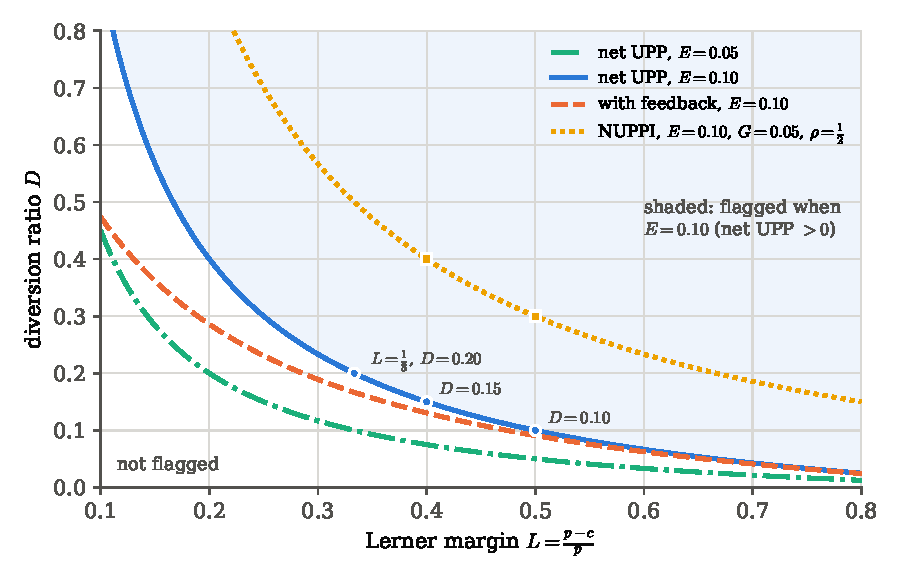
\includegraphics[width=0.86\textwidth]{figures/ch11/upp_thresholds.pdf}
\caption{UPP screening thresholds for a symmetric merger. Each curve gives the diversion ratio above which a test flags
the merger. The tests are net UPP with default efficiencies of 5 and 10 percent \eqref{eq:11-fs2}, the feedback test
\eqref{eq:11-fs4}, and the NUPPI test \eqref{eq:11-nuppi-sym} with $G = 0.05$ and $\rho = \frac{1}{2}$. The shaded
region is flagged by net UPP with $E = 0.10$. Circles mark the three cases in Farrell and Shapiro's fn.~43 and p.~17,
and squares mark their two NUPPI cases on p.~21.}
\label{fig:11-uppregion}
\end{figure}

\casehead{Extensions} The cannibalization logic extends in several directions
\citep[Sections 2.F and 7]{FarrellShapiro2010}. If firm A sells only product 1 while firm B sells products
$2, \dots, n$, the same derivation gives the tax
\begin{equation}\label{eq:11-upp-multi}
  t_1 = \sum_{j=2}^{n} D_{1j}\,(p_j - c_j) .
\end{equation}
When B's products have similar absolute margins, only the aggregate diversion from product 1 to B's group is needed.
If B sells a complement to product 1, say product 3, then $D_{13} < 0$. The merged firm then wants to lower $p_1$ to
spur sales of product 3, and the term $D_{13}(p_3 - c_3)$ offsets the pressure from substitutes. Follow-on revenues
enter through the margin. With spare parts, network effects, learning by doing or switching costs, a sale of product
2 today brings profits later, and the effective margin on product 2 exceeds $p_2 - c_2$. Accounting records sometimes
value these gains, and they usually make UPP for product 1 more likely.

Farrell and Shapiro derived \eqref{eq:11-upp} under static Bertrand pricing. If firms accommodate each other's price
changes before the merger, there is less competition for the merger to eliminate, and the compensating efficiency is
smaller. They still recommend the simple test, leaving non-Bertrand conduct to the rebuttal stage. Otherwise a merger
could permanently remove competition that the parties have only temporarily softened. Under Cournot competition, the
formula holds with a diversion ratio of one (their fn.~36). To see why, let A choose $q_1$ in a homogeneous-goods
market with inverse demand $P(Q)$. After the merger, A internalizes $\frac{d\pi_B}{dq_1} = q_2 P'(Q)$, because B's
quantity is fixed and only the price falls. The per-unit tax is $-q_2 P'(Q)$. B's Cournot condition
$P - c_2 + q_2 P'(Q) = 0$ gives $-q_2P'(Q) = P - c_2$, so $t_1 = 1 \cdot (P - c_2)$.

\casehead{Rebuttal} Farrell and Shapiro intend the test as a presumption that the merging parties can rebut
(their Section 4). The parties can dispute the inputs, for example by showing that marginal costs are closer to prices
or that efficiencies exceed the standard deduction. They can argue that pass-through is low, so that pressure moves
prices little. This argument is irrelevant to the pure sign test. When the test flags only one product, they can argue
that neither price will rise. They can also argue that the consumer gain from a price cut on the other product
outweighs the harm from the increase.
Finally, a full analysis can consider repositioning, entry and verified efficiencies.

\casehead{Interpretation} UPP reframes the loss of competition as an increase in the merged firm's opportunity cost.
That cost is directly comparable with marginal-cost savings. The test answers a narrow question: does the merger
change pricing incentives upward on balance at pre-merger prices? It does not predict magnitudes. In return it needs
only margins and diversion, both of which antitrust agencies often observe from documents and data, and it avoids
drawing market boundaries. Margins are hard to measure in cross-industry academic work, but firms track their own
costs closely, and agencies can obtain those records.

\casehead{Critiques} Without efficiencies, every merger of substitutes creates positive UPP. The policy content of the
test therefore lies in the standard deduction $E$, or in the threshold $G$ of the NUPPI variant below. These
parameters are not derived from evidence on merger efficiencies. Because the test is a sign test, it cannot rank
mergers by harm. Two mergers with equal UPP can have very different price effects when pass-through differs, a point
that motivates the first-order approach of \citet{JaffeWeyl2013}. The Bertrand assumption, the measurement of
marginal cost and the use of diversion at pre-merger prices are further sources of error. The test also ignores
repositioning and entry. \citet{MillerEtAl2017} compare UPP-based predictions with full merger simulations in
simulated industries.

\casehead{Contribution} Farrell and Shapiro made explicit the economic core of unilateral effects. A merger raises
the merged firm's effective marginal cost by the diversion-weighted margin of the partner product. They showed that the sign of the price effect is much easier to establish than its size. Their
framework, together with GUPPI, moved the analysis of unilateral effects away from market shares and toward diversion
and margins.

\subsection{From pricing pressure to price changes: pass-through}\label{sec:11-passthrough}

Under the conditions of \cref{prop:11-fs2}, the price effect of a merger equals the price response to a cost
increase on the merging products. That response is a \emph{pass-through rate}. It is the pass-through of a cost shock to some
products only, and it is an equilibrium rate, including rivals' responses. We first derive single-product pass-through
and then the multi-product approximation of \citet{JaffeWeyl2013}. \Cref{ch:theory} treats pass-through in general.

\begin{lemma}[Single-product pass-through]\label{lem:11-passthrough}
Let a firm face demand $q(p)$, holding rivals' prices fixed, with constant marginal cost $c$. Suppose the profit
maximizing price satisfies the first-order condition $q + (p - c)q' = 0$ and the second-order condition
$2q' + (p - c)q'' < 0$. Then
\begin{equation}\label{eq:11-passthrough}
  \rho = \frac{dp}{dc} = \frac{1}{2 + L\psi} , \qquad \psi = \frac{p\,q''(p)}{q'(p)} ,
\end{equation}
where $L = \frac{p - c}{p}$. Equivalently, with $\varepsilon(p) = -\frac{p\,q'(p)}{q(p)}$,
$\rho = \frac{\varepsilon}{\varepsilon - 1 + \frac{p}{\varepsilon}\frac{d\varepsilon}{dp}}$ \citep{BulowPfleiderer1983}.
\end{lemma}

\begin{proof}
Differentiate the first-order condition totally with respect to $p$ and $c$:
\begin{equation*}
  q'\,dp + q'\,(dp - dc) + (p - c)\,q''\,dp = 0 .
\end{equation*}
Collecting terms, $[2q' + (p-c)q'']\,dp = q'\,dc$, so $\rho = \frac{q'}{2q' + (p-c)q''}$. Dividing numerator and
denominator by $q'$, and writing $\frac{(p - c)q''}{q'} = \frac{p - c}{p}\cdot\frac{p\,q''}{q'} = L\psi$, gives
\eqref{eq:11-passthrough}. For the elasticity form, write the first-order condition as
$p\big[1 - \frac{1}{\varepsilon(p)}\big] = c$ and differentiate:
$\big[1 - \frac{1}{\varepsilon} + \frac{p}{\varepsilon^2}\frac{d\varepsilon}{dp}\big]dp = dc$. Solving for
$\frac{dp}{dc}$ and multiplying numerator and denominator by $\varepsilon$ gives the stated expression.
\end{proof}

Pass-through falls as demand becomes more elastic at higher prices. Three cases recur.

\begin{enumerate}[label=(\alph*)]
\item \emph{Linear demand.} Here $q'' = 0$, so $\psi = 0$ and $\rho = \frac{1}{2}$.
\item \emph{Constant elasticity.} With $q = k p^{-\varepsilon}$, $q' = -\varepsilon k p^{-\varepsilon - 1}$ and
      $q'' = \varepsilon(\varepsilon + 1)k p^{-\varepsilon - 2}$, so $\psi = -(\varepsilon + 1)$. The Lerner condition
      gives $L = \frac{1}{\varepsilon}$. Hence $\rho = \frac{1}{2 - \frac{\varepsilon + 1}{\varepsilon}} =
      \frac{\varepsilon}{\varepsilon - 1} = \frac{1}{1 - L} = \frac{p}{c} > 1$.
\item \emph{Logit, holding rivals' prices fixed.} The logit Lerner condition is $p - c = \frac{1}{\alpha(1 - s)}$.
      Differentiating, $dp - dc = \frac{1}{\alpha(1 - s)^2}\,ds$. Substituting $ds = -\alpha s(1 - s)\,dp$,
      \begin{equation*}
        dp - dc = -\frac{s}{1 - s}\,dp
        \quad\Longrightarrow\quad
        \frac{dp}{1 - s} = dc
        \quad\Longrightarrow\quad
        \rho = 1 - s .
      \end{equation*}
\end{enumerate}
Convex demand ($q'' > 0$, so $\psi < 0$) gives pass-through above one half, and concave demand gives less. Most
functional forms used in practice are convex.

Pass-through in oligopoly also depends on rivals' responses. In a Cournot market with linear inverse demand
$P = a - Q$ and $N$ active firms, firm $i$'s condition is $a - Q - q_i - c_i = 0$. Summing over firms gives
$Na - (N+1)Q = \sum_i c_i$, so $P = \frac{a + \sum_i c_i}{N + 1}$ and the pass-through of a firm-specific cost shock is
$\frac{1}{N+1}$ \citep{BergstromVarian1985}. With differentiated products the intuition that competitive industries
pass through little can fail. A firm facing very elastic residual demand prices close to cost before and after a cost
shock, so its pass-through is near one. Under constant elasticity it exceeds one \citep[Section 3.D]{FarrellShapiro2010}.

\casehead{The first-order approach} \citet{JaffeWeyl2013} turn \cref{prop:11-fs2} into an approximation. Divide each
first-order condition by $-\frac{\partial q_j}{\partial p_j}$ and write the pricing conditions in per-unit form,
\begin{equation}\label{eq:11-foa-f}
  f_j(p;\Omega) = p_j - c_j - \frac{q_j(p)}{-\frac{\partial q_j(p)}{\partial p_j}}
  - \sum_{k \ne j} \Omega_{jk}\, D_{jk}(p)\,(p_k - c_k) = 0 .
\end{equation}
For single-product firms before the merger the sum is empty. After the merger, the condition for product 1 gains the
term $D_{12}(p)(p_2 - c_2)$. Hence $f^{post}(p) = f^{pre}(p) - g(p)$, where $g(p)$ is the vector of generalized pricing
pressures. At the pre-merger prices $f^{pre}(p^0) = 0$, so $f^{post}(p^0) = -g(p^0)$, whose entries are $-\mathit{UPP}_j$
for the merging products and zero for others. A first-order expansion of $f^{post}(p^1) = 0$ around $p^0$ gives
\begin{equation*}
  0 = f^{post}(p^1) \approx f^{post}(p^0) + J^{post}\,(p^1 - p^0) , \qquad J^{post} = \frac{\partial f^{post}}{\partial p}(p^0) ,
\end{equation*}
and therefore
\begin{equation}\label{eq:11-foa}
  p^1 - p^0 \approx \big[J^{post}\big]^{-1} \mathit{UPP} \equiv \rho^{post}\, \mathit{UPP} .
\end{equation}
The matrix $\rho^{post}$ is a pass-through matrix. If each product's effective marginal cost rises by a per-unit amount
$\tau_j$, the conditions become $f^{post}(p) - \tau = 0$, and the implicit function theorem gives
$\frac{dp}{d\tau} = [J^{post}]^{-1}$. The merger price effect is approximately merger pass-through times UPP. Here $\tau$
shifts each normalized first-order condition directly. A rise in a physical marginal cost $c_k$ also changes the partner
term $D_{jk}(p_k - c_k)$. With $B_{jk} = \Omega_{jk}D_{jk}$ for $k \ne j$ and $B_{jj} = 0$,
\eqref{eq:11-foa-f} gives $f(p; c + \tau) = f(p; c) - (I - B)\tau$, so physical-cost pass-through is
$\frac{dp}{dc} = [J^{post}]^{-1}(I - B)$. The two coincide for single-product firms, where $B = 0$. The
pre-merger cost pass-through matrix $[J^{pre}]^{-1}$ can sometimes be estimated from past cost shocks. Jaffe and Weyl
propose using it in place of $\rho^{post}$ when demand curvature cannot be estimated directly. In the logit example of
\cref{sec:11-logitex}, the approximation \eqref{eq:11-foa} predicts a merging-firm price of 1.0648 with post-merger
pass-through and 1.0635 with pre-merger pass-through. The exact post-merger price is 1.0637.

\casehead{Curvature drives predictions} Because pass-through depends on second derivatives of demand, predicted merger
effects depend on curvature, which data rarely pin down. In practice curvature is set by the choice of functional
form. \citet{FroebTschantzWerden2005} simulated the proposed MCI and Sprint merger and found that constant-elasticity
demand predicted price effects over seven times larger than linear demand \citep[p.~19]{FarrellShapiro2010}. They also
noted that demand systems with higher pass-through of efficiencies predict larger price effects without efficiencies.
\Cref{prop:11-fs2} explains this pattern: both quantities are pass-through rates. \citet{CrookeEtAl1999} document the
same sensitivity across standard functional forms.

\Cref{fig:11-curvature} isolates the role of curvature. Two symmetric firms merge, and each demand system is calibrated
to the same price, marginal cost, own-price elasticity and diversion ratio at the pre-merger equilibrium. The
\emph{constant-expenditure logit} applies the logit formula, with log price in utility, to expenditure shares
(\cref{sec:11-bv}). Under linear, logit and constant-expenditure logit demand the merged firm's joint profit is
bounded. A grid search over both prices puts its global maximum at the symmetric solution of the first-order
conditions. The constant-expenditure logit, whose elasticities change little with price, predicts 2.4 to 3.3 times
the linear effect over the plotted range. Logit lies between linear and the constant-expenditure logit.

Constant-elasticity demand needs care. Hold $p_1 > c$ fixed and raise $p_2$. Then $q_1$ grows without bound, while
product 2 earns a nonnegative profit, so joint profit has no maximum for any $D > 0$. The figure therefore shows the
merged firm's optimum when it must charge one common price for both products. That price also solves the symmetric
first-order conditions that a merger simulation would solve. The implied price increase is 3.3 to 5.2 times the
linear effect. Without the restriction the symmetric solution is a strict local maximum of joint profit only for $D$
below about 0.25 and a saddle point above. Constant-elasticity demand is thus a local approximation, and its merger
predictions rely on that approximation far from observed prices.

The figure also plots the prediction obtained by freezing shares and slopes at their
pre-merger values, which we show in \cref{sec:11-simframework} equals the compensating cost reduction. Linear demand
predicts exactly half of it, because the symmetric linear pass-through of a cost shock to both products is one half.
\Cref{sec:11-bv} shows that the same issue separated the predictions of unit-demand and constant-expenditure
specifications in a merger of analgesics producers.

\begin{figure}[htbp]
\centering
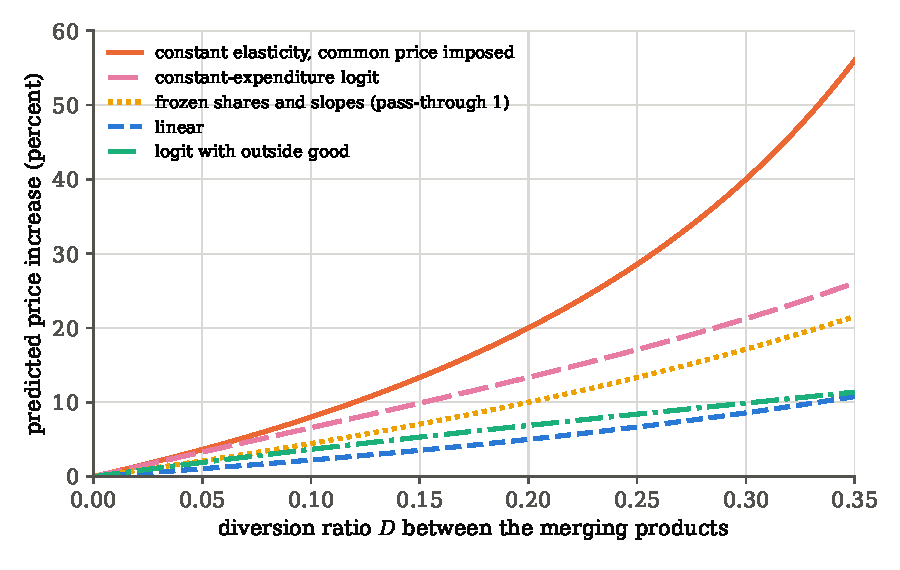
\includegraphics[width=0.86\textwidth]{figures/ch11/curvature_sim.pdf}
\caption{Predicted price increase from a merger of two symmetric single-product firms under four demand systems with
identical first derivatives at the pre-merger point. Calibration: $p = 1$, $c = 0.6$ ($L = 0.4$), own-price elasticity
$2.5$, diversion $D$ between the merging products on the horizontal axis, no efficiencies. Linear:
$q_j = a - b p_j + d p_k$ with $b = 2.5$ and $d = 2.5D$. Logit: one outside good, inside shares $\frac{D}{1+D}$.
Constant-expenditure logit: one outside good, value shares $w_j$ proportional to $p_j^{-\alpha}$ with
$\alpha = 1.5 + 2.5D$, and $q_j = \frac{B w_j}{p_j}$. Constant elasticity: $q_j = k p_j^{-2.5} p_k^{2.5 D}$, with the
merged firm restricted to one common price because its unrestricted joint profit is unbounded. The dotted line
freezes shares and slopes at pre-merger values, which gives $\frac{D L}{1 - D}$. Source: our calculations.}
\label{fig:11-curvature}
\end{figure}

\casehead{A significance threshold: NUPPI} Merger practice often asks first whether a merger without efficiencies would
cause a ``significant'' price increase, say a fraction $G$ of the price \citep[Section 3.C]{FarrellShapiro2010}. Let
$\rho_1$ be the equilibrium pass-through of a cost shock to product 1 alone. Internalizing the first-round tax raises
$p_1$ significantly if $\rho_1 t_1 > G p_1$. Dividing by $\rho_1 p_1$ gives inequality (5),
\begin{equation}\label{eq:11-fs5}
  D_{12}\,\frac{p_2 - c_2}{p_2}\,\frac{p_2}{p_1} > \frac{G}{\rho_1} ,
\end{equation}
which is $\mathit{GUPPI}_1 > \frac{G}{\rho_1}$. Adding the efficiency credit, $\rho_1[D_{12}(p_2 - c_2) - E c_1] > G p_1$,
which after dividing by $\rho_1 p_1$ becomes inequality (6),
\begin{equation}\label{eq:11-fs6}
  D_{12} L_2 \frac{p_2}{p_1} - E_1 (1 - L_1) > \frac{G}{\rho_1} .
\end{equation}
Farrell and Shapiro call the left side the \emph{net upward pricing pressure index} (NUPPI). In the symmetric case,
with $\rho$ the pass-through of a cost increase on both products,
\begin{equation}\label{eq:11-nuppi-sym}
  D L - E(1 - L) > \frac{G}{\rho} .
\end{equation}
Since $\rho$ is hard to estimate, a screen needs a default. They suggest $\rho = \frac{1}{2}$, the single-firm rate with
linear demand, which rivals' accommodation would raise (their fn.~59). With $G = 0.05$ and $\rho = \frac{1}{2}$, the
merger is presumed harmful when NUPPI is at least 10 percent. With $E = 0.10$, NUPPI equals $(D + 0.1)L - 0.1$, so the
condition is $(D + 0.1)L > 0.2$. A margin of 0.4 requires $D > 0.40$, and a margin of 0.5 requires $D > 0.30$
(p.~21). The NUPPI test is far more permissive than \eqref{eq:11-fs1}, especially with low assumed pass-through. It also
describes the roundabout way efficiencies enter merger review. Agencies first ask whether the merger without
efficiencies raises price significantly, which is \eqref{eq:11-fs6} with $E_1 = 0$ and needs a view on $\rho_1$. They
then ask whether efficiencies offset the gross pressure, which is \eqref{eq:11-fs6} with $G = 0$.

\casehead{UPP, simulation and market definition} Farrell and Shapiro compare their test with the two alternatives
(their Sections 5 and 6). Merger simulation must estimate the pass-through of the asymmetric cost shock in
\cref{prop:11-fs2}, explicitly or implicitly. Its predictions therefore depend heavily on the assumed demand system,
which invites a battle of experts. Simulation also tries to explain price levels, so it risks misspecification from
omitted features of conduct. UPP looks at the change in marginal incentives, which nets out features present before
and after the merger. Market definition is less different from simulation than it appears. The hypothetical monopolist
test simulates a merger of all products in a candidate market, and so it also hinges on pass-through. Only the sign
test avoids pass-through. Farrell and Shapiro suggest that a court could keep a broad market definition for context
while the government establishes its presumption through UPP within that market.

\section{Merger simulation}\label{sec:11-simulation}

Merger simulation predicts the post-merger equilibrium from an estimated model of demand and an assumed model of
conduct. \citet{BakerBresnahan1985}, \citet{HausmanLeonardZona1994} and \citet{WerdenFroeb1994} developed the approach
with residual demand, multi-level demand and logit demand. \citet{Nevo2000b} combined it with random coefficients
demand and computed full equilibria and welfare. This section sets out the general framework, works a logit example
in detail and then studies Nevo's application to ready-to-eat cereal.

\subsection{The framework}\label{sec:11-simframework}

Consider one market with $J$ products and market size $M$. Firm $f$ owns the products $\mathcal{J}_f$ and earns
\begin{equation*}
  \Pi_f = \sum_{j \in \mathcal{J}_f} (p_j - mc_j)\, M s_j(p) - C_f .
\end{equation*}
Under static multi-product Bertrand pricing (\cref{ch:diffprod,ch:blp}), the first-order condition for $j \in
\mathcal{J}_f$ is
\begin{equation}\label{eq:11-foc-multi}
  s_j(p) + \sum_{k \in \mathcal{J}_f} (p_k - mc_k)\frac{\partial s_k(p)}{\partial p_j} = 0 .
\end{equation}
Let $\Omega$ be the ownership matrix, with $\Omega_{jk} = 1$ when $j$ and $k$ have the same owner. Since the $(j,k)$
element of $\Delta^\top$ is $\frac{\partial s_k}{\partial p_j}$, stacking \eqref{eq:11-foc-multi} gives
\begin{equation}\label{eq:11-foc-matrix}
  s(p) + \big(\Omega \odot \Delta(p)^\top\big)(p - mc) = 0
  \quad\Longleftrightarrow\quad
  p = mc - \big(\Omega \odot \Delta(p)^\top\big)^{-1} s(p) .
\end{equation}
Because ownership is symmetric, $\Omega \odot \Delta^\top = (\Omega \odot \Delta)^\top$. \citet{Nevo2000b} writes the
same system with a matrix whose $(j,k)$ element is $-\frac{\partial s_j}{\partial p_k}$ for jointly owned products. That
is the transpose of ours. The difference is immaterial when the Jacobian is symmetric, as in logit, nested logit and
random coefficients logit with utility linear in price. It matters when price enters utility as $-\alpha \ln p_j$,
because then $\frac{\partial s_k}{\partial p_j} = \frac{\alpha s_j s_k}{p_j}$ is not symmetric.

\begin{assumption}[Merger simulation]\label{ass:11-sim}
(i) Demand is stable across the merger: the same function $s(p)$ applies before and after. (ii) Before the merger,
prices form a Bertrand-Nash equilibrium under $\Omega^{pre}$. (iii) After the merger, prices form a Bertrand-Nash
equilibrium under $\Omega^{post}$, which sets $\Omega_{jk} = 1$ for every pair of the merging firms' products.
(iv) Marginal costs are constant and unchanged by the merger unless efficiencies are imposed. (v) The set of products
and all non-price choices are fixed.
\end{assumption}

The algorithm has five steps.
\begin{enumerate}[label=(\arabic*)]
  \item Estimate demand on pre-merger data. This delivers $s(\cdot)$ and $\Delta(\cdot)$.
  \item Recover marginal costs from the pre-merger conditions,
        \begin{equation}\label{eq:11-mc-recover}
          \widehat{mc} = p^{pre} + \big(\Omega^{pre} \odot \Delta(p^{pre})^\top\big)^{-1} s(p^{pre}) .
        \end{equation}
  \item Replace $\Omega^{pre}$ by $\Omega^{post}$. Optionally lower the merging firms' costs to represent efficiencies.
  \item Solve \eqref{eq:11-foc-matrix} for the post-merger prices $p^*$ under $\Omega^{post}$ and the new costs.
  \item Compute the changes in prices, consumer surplus, profits and total welfare.
\end{enumerate}
Step 2 needs no cost data, but it relies on the pre-merger conduct assumption. \Cref{ch:blp} shows how cost shifters
can be added to estimate a supply side jointly with demand. \citet[eq.~(9)]{Nevo2000b} notes that
conduct parameters could multiply the entries of $\Omega$ and be estimated, but that this is hard in practice.

\casehead{The first iteration} Before Nevo's work, practitioners often reported an approximation instead of the
equilibrium \citep{HausmanLeonardZona1994,Werden1997}. It replaces the post-merger shares and derivatives by their
pre-merger values:
\begin{equation}\label{eq:11-approx}
  p^{approx} = \widehat{mc} - \big(\Omega^{post} \odot \Delta(p^{pre})^\top\big)^{-1} s(p^{pre})
\end{equation}
\citep[eq.~(11)]{Nevo2000b}. It is the first step of the fixed-point iteration on \eqref{eq:11-foc-matrix} started at
$p^{pre}$, so it captures the merged firm's direct incentive to raise price. The next result relates it to UPP.

\begin{proposition}[First iteration and compensating cost reductions]\label{prop:11-approx}
Let single-product firms 1 and 2 merge. The approximation \eqref{eq:11-approx} leaves every non-merging price unchanged.
For the merging products, $p_1^{approx} - p_1^{pre}$ and $p_2^{approx} - p_2^{pre}$ equal the compensating marginal
cost reductions $\Delta c_1$ and $\Delta c_2$ of \cref{prop:11-cmcr}.
\end{proposition}

\begin{proof}
Write $m = p^{pre} - \widehat{mc}$ for the pre-merger margins and $m' = p^{approx} - \widehat{mc}$. By step 2 and
\eqref{eq:11-approx}, both satisfy linear systems with the same right side:
\begin{equation*}
  \big(\Omega^{post} \odot \Delta^\top\big) m' = -s = \big(\Omega^{pre} \odot \Delta^\top\big) m ,
\end{equation*}
with $s$ and $\Delta$ at $p^{pre}$. Both matrices are block diagonal by owner. The blocks of non-merging firms coincide,
so their margins are unchanged. The merging block has rows
\begin{equation*}
  \frac{\partial s_1}{\partial p_1} m_1' + \frac{\partial s_2}{\partial p_1} m_2' = \frac{\partial s_1}{\partial p_1} m_1 , \qquad
  \frac{\partial s_1}{\partial p_2} m_1' + \frac{\partial s_2}{\partial p_2} m_2' = \frac{\partial s_2}{\partial p_2} m_2 .
\end{equation*}
Dividing the first row by $-\frac{\partial s_1}{\partial p_1}$ gives $-m_1' + D_{12} m_2' = -m_1$, so
$m_1' - m_1 = D_{12}\big(m_2 + (m_2' - m_2)\big)$. The second row gives $m_2' - m_2 = D_{21}\big(m_1 + (m_1' - m_1)\big)$.
These are the equations for $\Delta c_1$ and $\Delta c_2$ in the proof of \cref{prop:11-cmcr}, with margins
$p_j - c_j = m_j$. Their unique solution is \eqref{eq:11-cmcr}.
\end{proof}

The first iteration is therefore UPP with feedback between the merging products and with a pass-through of exactly
one. The compensating cost reduction is the cost cut that would offset the merger. The first iteration is the price
increase that the merger would cause if every unit of pricing pressure passed into price. The approximation overstates
the equilibrium effect when pass-through is below one, as with logit demand and small shares. It understates the effect
when pass-through exceeds one, as with the constant-expenditure logit of \cref{fig:11-curvature}.

\casehead{Computation} Solving \eqref{eq:11-foc-matrix} means solving $J$ nonlinear equations. The usual choice is a
Newton or quasi-Newton method applied to the first-order conditions, started from the pre-merger prices.
\citet[fn.~13]{Nevo2000b} used a standard nonlinear equation solver, and each city took several seconds on a 1997
personal computer. The naive iteration $p \leftarrow mc - (\Omega \odot \Delta(p)^\top)^{-1}s(p)$ need not converge.
\citet{MorrowSkerlos2011} propose a better-behaved fixed point for logit-type demand in which price enters utility as
$-\alpha_i p_j$. Decompose the Jacobian as $\Delta = \Lambda - \Gamma$, where the diagonal matrix $\Lambda$ has entries
$\Lambda_{jj} = -\int \alpha_i s_{ij}\,dP(i)$ and $\Gamma_{jk} = -\int \alpha_i s_{ij}s_{ik}\,dP(i)$. These two matrices
follow the notation of Morrow and Skerlos and are unrelated to the scalars $\Lambda$ of \cref{sec:11-fs} and $\Gamma$
of \cref{sec:11-dd}. Substituting into \eqref{eq:11-foc-matrix} and using $\Omega \odot \Lambda = \Lambda$,
\begin{equation}\label{eq:11-zeta}
  p = mc + \zeta(p) , \qquad \zeta(p) = \Lambda(p)^{-1}\big[\big(\Omega \odot \Gamma(p)^\top\big)(p - mc) - s(p)\big] .
\end{equation}
They report that iterating on this map is fast and reliable in large problems, and \texttt{pyblp} uses it
(\cref{ch:blp}). Existence and uniqueness of the post-merger equilibrium are not automatic. The log-concavity
conditions of \citet{CaplinNalebuff1991} give existence for broad classes of discrete choice demand when each firm
sells one product (\cref{thm:04-cn-existence}). Their uniqueness results cover only restricted cases, such as the
logit and duopoly (\cref{sec:04-uniqueness}). A merger creates a multiproduct firm, which their theorems do not cover.
With logit demand, uniqueness holds for every ownership structure (\cref{thm:04-logit-unique}). Random coefficients
demand with multiproduct firms has no such theorem. In practice one checks that the solver reaches the same prices
from several starting points.

\casehead{Calibration} The simulated pre-merger prices must equal observed prices, so that the simulation compares the
merger with the status quo. In a logit model one can add a residual to predicted shares. \citet[p.~31]{Nevo2000b}
points out that with heterogeneous consumers this can make individual purchase probabilities negative. He adds the
estimated residual $\xi$ to utility instead, so that the model reproduces observed shares exactly.

\casehead{Welfare} With utility linear in price and type I extreme value errors, the expected consumer surplus of
consumer $i$, up to a constant, is
\begin{equation}\label{eq:11-cs}
  \mathit{CS}_i = \frac{1}{\alpha_i}\ln\Big(1 + \sum_{j=1}^{J} e^{V_{ij}}\Big) .
\end{equation}
Here $V_{ij}$ is the deterministic part of utility from product $j$. The outside good has $V_{i0} = 0$
\citep{SmallRosen1981,Trajtenberg1989}. The log-sum is the expected maximum utility. Dividing by $\alpha_i$, the
marginal utility of income, converts it into money (\cref{ch:logit}). The change in consumer surplus is
\begin{equation}\label{eq:11-dcs}
  \Delta \mathit{CS} = M\,\frac{1}{n_s}\sum_{i=1}^{n_s} \frac{1}{\alpha_i}
  \Big[\ln\Big(1 + \sum_j e^{V_{ij}^{post}}\Big) - \ln\Big(1 + \sum_j e^{V_{ij}^{pre}}\Big)\Big] ,
\end{equation}
averaging over $n_s$ simulated consumers. With plain logit, $\alpha_i = \alpha$ and the average has one term. The change
in producer surplus is $\sum_j (p_j^{post} - mc_j^{post}) M s_j^{post} - \sum_j (p_j^{pre} - mc_j^{pre}) M s_j^{pre}$,
since fixed costs are unchanged. Total welfare changes by the sum.

\casehead{Partial internalization} The framework accommodates objectives that place weight on other firms' profits.
Suppose firm $f$ maximizes $\Pi_f + \sum_{g \ne f} \kappa_{fg}\Pi_g$. The first-order condition keeps the form
\eqref{eq:11-foc-matrix} with $\Omega_{jk}(\kappa) = \kappa_{fg}$ for $j \in \mathcal{J}_f$ and $k \in \mathcal{J}_g$.
With partial ownership, \citet{OBrienSalop2000} derive the weights from financial interests and control rights.
\citet{MillerWeinberg2017} use a common weight $\kappa$ to measure coordination between two firms after a joint venture
(\cref{sec:11-millercoors}). When $\kappa_{fg} \ne \kappa_{gf}$, $\Omega$ is not symmetric, and the form
$\Omega \odot \Delta^\top$ in \eqref{eq:11-foc-matrix} must be used.

\casehead{Caveats} A simulation is only as good as the demand model. Functional form fixes curvature and hence
pass-through (\cref{sec:11-passthrough}). Simulation also relies on assumptions about post-merger conduct: joint profit
maximization, unchanged behavior of rivals, a stable demand system and predictable efficiencies. Nevo stresses that
$\Omega^{pre}$ and $\Omega^{post}$ use the same demand estimates. This is inconsistent with firms changing other choices
that affect demand. If advertising changes after the merger and affects $\frac{\partial s}{\partial p}$, the predicted
prices are wrong. Product repositioning, entry and new products are absent from the static model
\citep[pp.~23--25]{Nevo2000b}. Finally, the exercise is data-intensive and time-consuming, which matters under the
statutory deadlines of merger review.

\subsection{A worked example with logit demand}\label{sec:11-logitex}

The following example traces every concept of this section and \cref{sec:11-upp} through one calibrated market. The
calibration is the one \citet[p.~1780]{MillerWeinberg2017} use to illustrate their internalization parameter. All
numbers are our computations.

\begin{example}[Logit merger simulation]\label{ex:11-logit}
Three symmetric single-product firms sell at $p = 1$ with marginal cost $c = 0.7$. Each has share $s = 0.2$, and the
outside good has $s_0 = 0.4$. Market size is one. Demand is logit, and pre-merger prices are a Bertrand-Nash
equilibrium. Firms 1 and 2 merge.

\emph{Calibration.} The logit Lerner condition $p - c = \frac{1}{\alpha(1 - s)}$ gives
$\alpha = \frac{1}{0.3 \times 0.8} = 4.1667$. Mean utilities satisfy $e^{\delta_j} = \frac{s_j}{s_0} = 0.5$.

\emph{Screening statistics.} Diversion is $D_{12} = \frac{0.2}{1 - 0.2} = 0.25$, and diversion to the outside good is
$\frac{0.4}{0.8} = 0.5$. Upward pricing pressure is $\mathit{UPP}_1 = 0.25 \times 0.3 = 0.075$, so
$\mathit{GUPPI}_1 = 7.5$ percent. With $L = 0.3$ and $E = 0.10$, the simple test requires
$D > \frac{0.1 \times 0.7}{0.3} = 0.233$, which holds narrowly. Net UPP is $0.075 - 0.07 = 0.005$. The feedback test
compares $\frac{D}{1 - D} = 0.333$ with $0.233$ and flags the merger clearly. By \eqref{eq:11-cmcr}, the compensating
cost reduction is
\begin{equation*}
  \Delta c = \frac{0.25 \times 0.3 + 0.0625 \times 0.3}{1 - 0.0625} = 0.100 ,
\end{equation*}
which is 14.3 percent of marginal cost. A 10 percent standard deduction falls short.

\emph{Approximations.} Holding the rival's price fixed, single-product logit pass-through is $1 - s = 0.8$, so
$\rho\,\mathit{UPP} = 0.06$. The first iteration \eqref{eq:11-approx} gives $p_1 = p_2 = 1.100$ and $p_3 = 1$, the
compensating reduction of \cref{prop:11-approx}. The first-order approach \eqref{eq:11-foa} gives 1.0648 with
post-merger pass-through and 1.0635 with pre-merger pass-through. Farrell and Shapiro's iterative tax procedure
converges within three rounds. The first round imposes taxes of 0.075 and yields prices of 1.0641. The second round
lowers the taxes to 0.0745 and the prices slightly, to 1.0637. The third round changes neither at four decimals. The
limiting tax of
\cref{prop:11-fs2} is $t^* = 0.2049 \times 0.3637 = 0.0745$. It is slightly below the first-round tax: the margin rises,
but diversion falls from 0.25 to 0.2049 as the merging products' shares fall.

\emph{Full simulation.} The post-merger equilibrium prices are $(1.0637, 1.0637, 1.0062)$. The merging firms raise
prices by 6.4 percent and the rival by 0.6 percent. The merged firm's markup of 0.3637 equals the multi-product logit
common markup $\frac{1}{\alpha(1 - S_f)}$ with combined share $S_f = 0.3402$ (\cref{ch:diffprod,app:problems}). Consumer
surplus falls by 0.0249, against pre-merger revenue of 0.6. The merged firm's profit rises by 0.0037, and the rival's by
0.0062. Total welfare falls by 0.0149.

\emph{Efficiencies.} If the merger lowers the merging firms' cost to $0.7 - 0.1 = 0.6$, the post-merger equilibrium is
the pre-merger price vector. Consumers are unaffected, and total welfare rises by the cost saving of 0.04.

\emph{Partial internalization.} Suppose the merged firm and firm 3 each place weight $\kappa = 0.5$ on the other's
profit. Then prices rise to $(1.1040, 1.1040, 1.0731)$, and consumer surplus falls by 0.0515, about twice the loss
under unilateral effects alone. With the merging firms' cost cut to 0.5, prices are $(0.9834, 0.9834, 1.1028)$. The
efficiency lowers the merging firms' prices but raises firm 3's. The merging products' margins grow, and firm 3
internalizes half of them. Consumer surplus is unchanged only if the merging firms' cost falls to 0.4532, a 35.3
percent reduction, against 14.3 percent without coordination.
\end{example}

\begin{table}[htbp]
\centering
\caption{Logit merger example: prices, outside share and welfare changes}
\label{tab:11-logitex}
\small
\begin{tabular}{@{}lccccccc@{}}
\toprule
Scenario & $p_1 = p_2$ & $p_3$ & $s_0$ & $\Delta\mathit{CS}$ & $\Delta\pi_{1+2}$ & $\Delta\pi_3$ & $\Delta W$ \\
\midrule
Pre-merger                                   & 1.0000 & 1.0000 & 0.4000 & 0       & 0       & 0       & 0       \\
First iteration \eqref{eq:11-approx}         & 1.1000 & 1.0000 &        &         &         &         &         \\
First-order approach \eqref{eq:11-foa}       & 1.0648 & 1.0065 &        &         &         &         &         \\
Merger, $\kappa = 0$                         & 1.0637 & 1.0062 & 0.4436 & $-0.0249$ & 0.0037 & 0.0062 & $-0.0149$ \\
Merger, $\kappa = 0$, $c_{1,2} = 0.6$         & 1.0000 & 1.0000 & 0.4000 & 0.0000  & 0.0400  & 0.0000  & 0.0400  \\
Merger, $\kappa = 0.5$                       & 1.1040 & 1.0731 & 0.4958 & $-0.0515$ & 0.0099 & 0.0082 & $-0.0335$ \\
Merger, $\kappa = 0.5$, $c_{1,2} = 0.68$      & 1.0907 & 1.0755 & 0.4877 & $-0.0476$ & 0.0173 & 0.0069 & $-0.0235$ \\
Merger, $\kappa = 0.5$, $c_{1,2} = 0.5$       & 0.9834 & 1.1028 & 0.4171 & $-0.0101$ & 0.0961 & $-0.0053$ & 0.0807 \\
Merger, $\kappa = 1$                         & 1.1405 & 1.1405 & 0.5449 & $-0.0742$ & 0.0137 & 0.0068 & $-0.0537$ \\
\bottomrule
\end{tabular}

\smallskip
\begin{minipage}{0.95\linewidth}
\footnotesize
Notes: Three symmetric firms with $p = 1$, $c = 0.7$, $s = 0.2$, $s_0 = 0.4$ and $\alpha = 4.1667$ before the merger.
Firms 1 and 2 merge. $\kappa$ is the weight that the merged firm and firm 3 place on each other's profit. $c_{1,2}$ is
the merging firms' post-merger marginal cost (0.7 unless stated). Welfare changes are per unit of market size and in
units of price, with consumer surplus from \eqref{eq:11-dcs}. The first-order approach row uses post-merger
pass-through. Source: our calculations.
\end{minipage}
\end{table}

\begin{figure}[htbp]
\centering
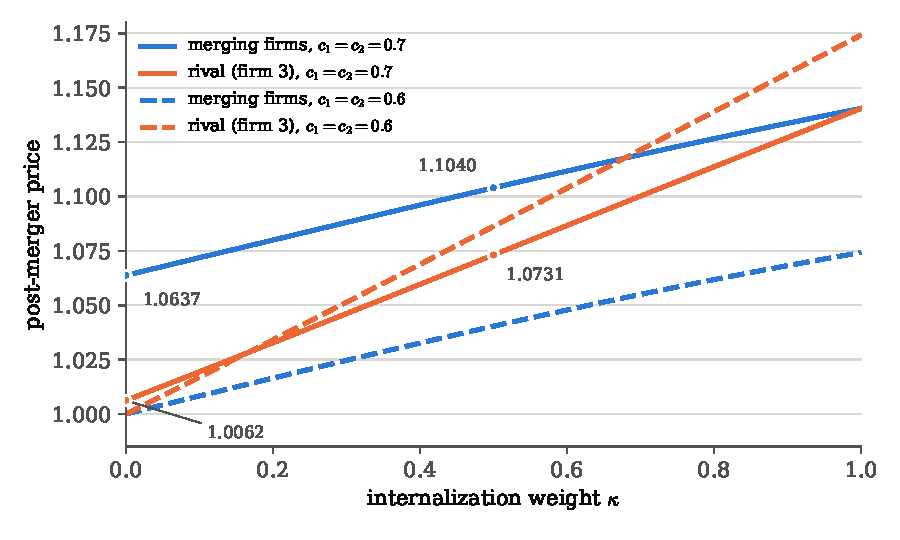
\includegraphics[width=0.86\textwidth]{figures/ch11/logit_kappa.pdf}
\caption{Post-merger prices in the logit example as a function of the internalization weight $\kappa$ between the
merged firm and firm 3. Solid lines keep the merging firms' marginal cost at 0.7, and dashed lines lower it to 0.6, the
compensating cost reduction. Dots mark $\kappa = 0$ and $\kappa = 0.5$. Source: our calculations.}
\label{fig:11-kappa}
\end{figure}

\Cref{fig:11-kappa} shows how $\kappa$ separates unilateral from coordinated effects. At $\kappa = 0$ the rival's price
barely moves, since its response comes only through strategic complementarity. As $\kappa$ rises, the rival's price
rises nearly linearly, and at $\kappa = 1$ the industry behaves as a monopoly. With the compensating cost reduction
(dashed lines), merging prices stay at one when $\kappa = 0$, but coordination still raises all prices. Efficiencies
can offset unilateral effects, but they do not offset coordinated effects. The rival's price is the observable that
distinguishes the two. \citet{MillerWeinberg2017} build their identification argument for $\kappa$ on this contrast
(\cref{sec:11-millercoors}).

\begin{remark}[The third case in Miller and Weinberg's illustration]\label{rem:11-mw-typo}
\citet[p.~1780]{MillerWeinberg2017} report post-merger prices of about 1.06, 1.06 and 1.01 at $\kappa = 0$ and about
1.10, 1.10 and 1.07 at $\kappa = 0.5$, which match our calculations.
For $\kappa = 0.5$ with the merging firms' marginal cost lowered to 0.50, the text reports prices of 1.09, 1.09 and 1.08.
We obtain $(0.9834, 0.9834, 1.1028)$ for that case. The reported values correspond to a merging-firm cost of about
0.68. We obtain a merging price of 1.09 at a cost of 0.679, with the rival at 1.0756. \Cref{sec:11-mc-theory}
inverts both reported prices jointly for $\kappa$ and the merging firms' cost.
\end{remark}

\subsection{Nevo (2000): mergers in ready-to-eat cereal}\label{sec:11-nevo}

\casehead{The question} \citet{Nevo2000b} asks whether a flexible demand model, estimated with standard scanner data,
can discipline merger analysis in a concentrated industry with many differentiated products. He also asks how much the
answer depends on two choices: the demand model and the decision to compute the full post-merger equilibrium instead of
an approximation. Nevo frames merger simulation as the analogue of market definition. The ``front end'' estimates
demand, and the ``back end'' simulates the merger. He argues that the debate should focus on the front end, because
the demand estimates largely determine the outcome. The working paper (November 1997) was published in the RAND
Journal of Economics in 2000. Our equation and table numbers follow the working paper.

\casehead{The critique of traditional analysis} Nevo describes the screen of the 1982 and 1984 Guidelines (printed
pp.~5--6). A merger was not challenged if the post-merger HHI was below 1,000. Between 1,000 and 1,800, increases below 100 points
were usually not challenged. Above 1,800, an increase of 50 points was the threshold for a challenge. He argues that
concentration indices measure competitive effects well only if products are equally spaced in characteristics. Under
logit demand, substitution depends only on shares, and share-based policy is then sensible \citep{Willig1991}. For
cereal, logit is inadequate. Consumer heterogeneity also makes it easy to argue that hot cereal or bagels belong in
the market, which yields broad markets and small shares. The 1992 Guidelines introduced unilateral effects, and
\citet{Shapiro1996} described their implementation through diversion ratios and margins. Practice then moved to
computing price increases from estimated elasticities, usually with an approximation.

\casehead{Demand options} With $J$ products, an unrestricted demand system has on the order of $J^2$ price
parameters. With 200 cereal brands and constant elasticities, that is 40,000 elasticities. Nevo discusses three
solutions (his Section 3.1).
\begin{enumerate}[label=(\alph*)]
  \item \emph{Symmetric representative-consumer models.} The CES utility of \citet{DixitStiglitz1977} imposes equal
        cross-price elasticities. The representative-consumer form of logit has utility
        $\sum_i a_i q_i - \sum_i q_i \ln q_i$ \citep{AndersonDePalmaThisse1992}. Its entropy term treats all products
        symmetrically, so substitution depends only on shares.
  \item \emph{Multi-stage budgeting} \citep{HausmanLeonardZona1994}. The bottom level is an AIDS model for brand $j$ in
        segment $g$, city $c$ and quarter $t$ (\cref{ch:aids}),
        \begin{equation}\label{eq:11-nevo-aids}
          s_{jct} = \alpha_{jc} + \beta_j \ln\Big(\frac{y_{gct}}{P_{gct}}\Big) + \sum_{k=1}^{J} \gamma_{jk}\ln p_{kct} + \varepsilon_{jct} .
        \end{equation}
        Here $s_{jct}$ is the dollar share of segment expenditure $y_{gct}$ (his eq.~(1)). The price index is the Stone
        index $\ln P_{gct} = \sum_{k \in g} s_{kct}\ln p_{kct}$ (eq.~(2)) or the exact AIDS index (eq.~(3)). A middle
        level allocates expenditure across segments, for example with the log-log form
        $\ln q_{gct} = \beta_g \ln y_{Rct} + \sum_{k} \gamma_k \ln \pi_{kct} + \alpha_{gc} + \varepsilon_{gct}$. A top
        level gives total cereal demand. Nevo notes that the middle levels used in practice do not satisfy the
        conditions for exact two-stage budgeting.
  \item \emph{Discrete choice} \citep{Berry1994,BerryLevinsohnPakes1995}. Products are projected onto a space of
        characteristics, so the number of parameters grows with the number of characteristics.
\end{enumerate}
He rules out the symmetric models for merger work unless time is binding. Multi-level models need an a priori
segmentation into small groups and assume that every consumer buys every variety. They are closer to classical demand
theory and faster to compute. Discrete choice models need product characteristics and distributional assumptions, and
they are computationally heavier.

\casehead{The industry} Ready-to-eat cereal has high concentration, high price-cost margins, high advertising to
sales ratios and frequent product introductions. Concentration is high at the firm level and lower at the brand level.
The leading brands have about 5 percent of the market and the smaller brands in the sample about 1 percent.
\Cref{tab:11-nevo-shares} reports firm shares. Kellogg's volume share fell from 41.4 percent in the first quarter of
1988 to 33.7 percent in the last quarter of 1992, while General Mills rose from 22.0 to 26.8 percent. The three-firm
concentration ratio stayed above 70 percent throughout. Private labels grew from 3.3 to 7.6 percent of volume.

\begin{table}[htbp]
\centering
\caption{Firm shares in ready-to-eat cereal, 1988--1992, in percent (Nevo 1997 working paper, Tables 1A and 1B)}
\label{tab:11-nevo-shares}
\small
\begin{tabular}{@{}lcccccc@{}}
\toprule
 & \multicolumn{3}{c}{Volume shares} & \multicolumn{3}{c}{Sales shares} \\
\cmidrule(lr){2-4}\cmidrule(lr){5-7}
 & 88Q1 & 90Q4 & 92Q4 & 88Q1 & 90Q4 & 92Q4 \\
\midrule
Kellogg        & 41.39 & 37.86 & 33.70 & 41.23 & 37.26 & 32.57 \\
General Mills  & 22.04 & 23.82 & 26.83 & 24.73 & 27.70 & 31.39 \\
Post           & 11.80 & 10.96 & 11.31 & 11.15 & 10.56 & 10.97 \\
Quaker Oats    &  9.93 &  7.66 &  7.40 &  9.46 &  7.30 &  6.94 \\
Ralston        &  4.86 &  6.60 &  5.18 &  5.12 &  7.03 &  5.45 \\
Nabisco        &  5.32 &  3.75 &  3.11 &  5.00 &  3.58 &  3.33 \\
\midrule
C3             & 75.23 & 72.64 & 71.84 & 77.11 & 75.52 & 74.93 \\
C6             & 95.34 & 90.65 & 87.53 & 96.69 & 93.43 & 90.65 \\
Private label  &  3.33 &  6.29 &  7.60 &  2.12 &  3.74 &  4.55 \\
\bottomrule
\end{tabular}

\smallskip
\begin{minipage}{0.86\linewidth}
\footnotesize
Notes: C3 and C6 are the combined shares of the three and six largest firms. The paper also reports 88Q4, 89Q4 and
91Q4. Source: \citet{Nevo2000b}, working paper Tables 1A and 1B, from IRI Infoscan data.
\end{minipage}
\end{table}

\casehead{Data} Shares and prices come from the IRI Infoscan database, collected by scanners in a national random sample
of supermarkets. The sample represents supermarkets with annual sales above \$2 million, which account for 82 percent of
US grocery sales. Data are aggregated to the brand, city and quarter. The sample has 24 brands, listed by segment in his
Table 2: all-family or basic, taste-enhanced wholesome, simple health nutrition, and kids. The estimation sample
covers 45 cities and 20 quarters from 1988 to 1992, so it has $24 \times 45 \times 20 = 21{,}600$ observations in 900
city-quarter markets. Quantity
is converted into servings. Market size is one serving per capita per day, and the outside share is the remainder. Price
is dollar sales divided by servings, deflated by a regional urban CPI. It is the average transaction price at the
register, before any coupons redeemed after purchase.

Advertising comes from the Leading National Advertisers database, summed over ten media. Nevo collected
characteristics from cereal boxes: calories from fat, sugar, fiber, segment dummies and a ``mushy'' dummy for cereals
that turn soggy in milk. Demographics are drawn from the March Current Population Survey (CPS): income per person
(household income divided by household size), age and a child dummy. Instruments use supermarket-sector wages by city
from CPS earnings files, city density, and regional price indices from the Bureau of Labor Statistics.

\casehead{The model} The indirect utility of consumer $i$ from brand $j$ in market $t$ is (his eq.~(4), in our sign
convention)
\begin{equation}\label{eq:11-nevo-u}
  u_{ijt} = x_{jt}\beta_i - \alpha_i p_{jt} + \xi_j + \Delta\xi_{jt} + \epsilon_{ijt} .
\end{equation}
Here $\xi_j$ is the national mean of unobserved quality and $\Delta\xi_{jt}$ the market-specific deviation. Tastes
depend on demographics $D_i$ and unobserved draws $\nu_i$ (eq.~(5)),
\begin{equation}\label{eq:11-nevo-rc}
  \begin{pmatrix} \alpha_i \\ \beta_i \end{pmatrix}
  = \begin{pmatrix} \alpha \\ \beta \end{pmatrix} + \Pi D_i + \Sigma \nu_i , \qquad \nu_i \sim N(0, I_{K+1}) .
\end{equation}
The outside good gives $u_{i0t} = \xi_0 + \pi_0 D_i + \sigma_0 \nu_{i0} + \epsilon_{i0t}$, with $\xi_0$ normalized to zero.
Setting $\Pi = 0$ and $\Sigma = 0$ gives the logit model (eq.~(6)), $u_{ijt} = x_{jt}\beta - \alpha p_{jt} + \xi_j +
\Delta\xi_{jt} + \epsilon_{ijt}$. Nevo stresses two logit restrictions. Cross-price elasticities follow shares. Own-price
elasticities are nearly proportional to price when shares are small, so cheaper brands get higher percentage markups.
With random coefficients, the own elasticity averages heterogeneous price sensitivities with purchase probabilities as
weights, and substitution follows characteristics. The supply side is multi-product Bertrand pricing as in
\eqref{eq:11-foc-matrix}.

\casehead{Estimation} The logit model is estimated from the Berry inversion,
\begin{equation}\label{eq:11-nevo-logit}
  \ln S_{jt} - \ln S_{0t} = d_j + x_{jt}\beta - \alpha p_{jt} + \tau_t + \Delta\xi_{jt} ,
\end{equation}
where $d_j$ are brand dummies, $\tau_t$ quarter dummies and $x_{jt}$ includes advertising and, in some columns, city
demographics. The full model is estimated by GMM following \citet{Berry1994} and \citet{BerryLevinsohnPakes1995}. For
given nonlinear parameters $\theta_2 = (\Pi, \Sigma)$, invert the share equations $s_{\cdot t}(\delta_{\cdot t};\theta_2)
= S_{\cdot t}$ market by market to recover mean utilities $\delta_{jt}(S_{\cdot t};\theta_2)$. The structural error is
(his eq.~(17))
\begin{equation*}
  \Delta\xi_{jt}(\theta) = \delta_{jt}(S_{\cdot t};\theta_2) - \big(d_j + x_{jt}\beta - \alpha p_{jt}\big) .
\end{equation*}
With instruments $Z$ satisfying $\E[Z^\top \Delta\xi(\theta^*)] = 0$ (eq.~(15)), the estimator is
\begin{equation*}
  \hat\theta = \argmin_\theta\ \Delta\xi(\theta)^\top Z \hat A^{-1} Z^\top \Delta\xi(\theta) ,
\end{equation*}
with $\hat A$ a consistent estimate of $\E[Z^\top \Delta\xi\Delta\xi^\top Z]$ (eq.~(16)). For logit, with $\hat A = Z^\top Z$, this is two-stage
least squares. \Cref{ch:blp} develops the algorithm.

Brand dummies absorb both $x_j\beta$ and $\xi_j$, so the error is the city-quarter deviation $\Delta\xi_{jt}$. The mean
tastes for fixed characteristics are recovered by minimum distance \citep{Chamberlain1982}. Let $\hat d$ be the
estimated brand dummies with covariance matrix $V_d$, and let $X$ be the $J \times K$ characteristics matrix. Since
$d = X\beta + \xi$,
\begin{equation*}
  \hat\beta = \big(X^\top V_d^{-1} X\big)^{-1} X^\top V_d^{-1} \hat d , \qquad \hat\xi = \hat d - X\hat\beta .
\end{equation*}
A $\chi^2$ statistic tests the restriction that $\xi = 0$.

\casehead{Instruments and identification} Prices respond to the unobserved demand shock. Nevo decomposes price into
marginal cost and markup, each with a national brand component and a city-quarter deviation (his eq.~(18)). Brand
dummies absorb the national components. The remaining deviation $\Delta\xi_{jt}$ is observed by firms and raises the
local markup, which biases the price coefficient toward zero. The main instruments exploit the panel. The identifying
assumption is that, conditional on brand means and demographics, city-specific valuations are independent across
cities, though possibly correlated over time within a city. Prices of the same brand in other cities then share the
marginal cost component but not the demand shock. Nevo uses regional quarterly average prices, excluding the city being
instrumented. This is the same idea as the instruments of \citet{Hausman1997} and \citet{Nevo2001} (\cref{ch:blp}). The
assumption fails if demand shocks are correlated across cities, for example through national advertising campaigns.
Nevo therefore also uses direct cost proxies. Production and packaging costs vary little across cities, so the proxies
target distribution costs: region dummies for transport costs, city density for the cost of space, and supermarket wages.

\casehead{Logit results} \Cref{tab:11-nevo-logit} reproduces his Table 3. The OLS price coefficient is $-8.57$, and
the implied mean own elasticity is $-1.71$, with 4.4 percent of brand-city-quarter demands inelastic. Such demands are
inconsistent with profit maximization. Instrumenting raises the price coefficient in absolute value to $-12.60$ with
regional prices and $-12.65$ with cost proxies. The two sets of instruments give nearly identical estimates. Adding
city demographics raises it further, to $-16.61$ and $-16.97$ with each instrument set alone and to $-18.21$ when
both sets are used. No demand is
inelastic once prices are instrumented. The overidentification tests reject in every IV column, however, and Nevo notes
reasons to doubt the instruments' validity. He reads the similarity across instrument sets as encouraging, without
claiming that it proves validity.

\begin{table}[htbp]
\centering
\caption{Logit demand estimates, 21,600 observations (Nevo 1997 working paper, Table 3)}
\label{tab:11-nevo-logit}
\small
\setlength{\tabcolsep}{4.5pt}
\begin{tabular}{@{}lcccccc@{}}
\toprule
 & OLS & \multicolumn{5}{c}{IV} \\
\cmidrule(lr){3-7}
 & (i) & (ii) & (iii) & (iv) & (v) & (vi) \\
\midrule
Price                  & $-8.57$ & $-12.60$ & $-12.65$ & $-16.61$ & $-16.97$ & $-18.21$ \\
                       & (0.179) & (0.436)  & (0.467)  & (0.443)  & (0.483)  & (0.439)  \\
Advertising            & 0.034   & 0.032    & 0.032    & 0.030    & 0.030    & 0.030    \\
                       & (0.002) & (0.002)  & (0.002)  & (0.002)  & (0.002)  & (0.002)  \\
Log median income      &         &          &          & 0.99     & 1.00     & 1.01     \\
                       &         &          &          & (0.021)  & (0.022)  & (0.022)  \\
Log median age         &         &          &          & $-0.02$  & 0.01     & 0.04     \\
                       &         &          &          & (0.06)   & (0.06)   & (0.06)   \\
Median household size  &         &          &          & $-0.03$  & $-0.02$  & $-0.02$  \\
                       &         &          &          & (0.03)   & (0.03)   & (0.03)   \\
\midrule
Fit or overidentification & 0.76 & 99.1     & 98.7     & 59.0     & 51.3     & 54.8     \\
                       &         & (30.1)   & (16.9)   & (30.1)   & (16.9)   & (42.6)   \\
First-stage $R^2$      &         & 94.5     & 94.4     & 94.5     & 94.5     & 94.7     \\
First-stage $F$        &         & 5179     & 6740     & 5046     & 6483     & 4959     \\
Regional prices as IV  &         & yes      &          & yes      &          & yes      \\
Cost proxies as IV     &         &          & yes      &          & yes      & yes      \\
\midrule
Own elasticity: mean   & $-1.71$ & $-2.51$  & $-2.51$  & $-3.31$  & $-3.38$  & $-3.62$  \\
Own elasticity: s.d.   & 0.51    & 0.75     & 0.75     & 0.99     & 1.01     & 1.09     \\
Own elasticity: median & $-1.60$ & $-2.36$  & $-2.36$  & $-3.11$  & $-3.18$  & $-3.41$  \\
Inelastic demands (\%) & 4.4     & 0        & 0        & 0        & 0        & 0        \\
\bottomrule
\end{tabular}

\smallskip
\begin{minipage}{0.95\linewidth}
\footnotesize
Notes: Dependent variable $\ln S_{jt} - \ln S_{0t}$. All regressions include brand and time dummies. Robust standard
errors in parentheses. The fit row reports the adjusted $R^2$ for OLS and the overidentification statistic of
\citet{Hausman1983} for the IV columns, with the 95 percent cutoff of its $\chi^2$ distribution in parentheses. The share of
inelastic demands under OLS has a $\pm 2$ standard error band of 4.1 to 4.9 percent. Coefficients are on price as it
enters utility, so $-\alpha$ in our notation. Source: \citet{Nevo2000b}, working paper Table 3.
\end{minipage}
\end{table}

Logit elasticities show both restrictions that Nevo emphasizes (his Table 4). Own elasticities are almost exactly
linear in price. Dividing each own elasticity by the brand's median price per serving gives roughly 16 per dollar for
every brand. The ratio is 16.4 for Kellogg's Corn Flakes, 16.2 for Cracklin' Oat Bran and 15.7 for Raisin Nut (our
calculation from his Tables 4 and 7). This is $\alpha(1 - s_j)$ with small shares, close to the IV estimates of $\alpha$ in columns (iv)
and (v). Cross elasticities with respect to a given brand's price are identical for all other brands. A one percent
rise in the price of Cheerios raises every other brand's share by 0.051 percent, whether that brand is Honey Nut
Cheerios or Grape Nuts.

\casehead{Random coefficients results} \Cref{tab:11-nevo-rc} reproduces his Table 5. The price coefficient has mean
$-23.202$ and interacts strongly with demographics. Price sensitivity falls with income at a decreasing rate (318.774
on income and $-18.243$ on income squared), and the presence of children raises it ($-10.664$). The standard deviation
of the unobserved price taste is small and insignificant, so demographics explain most of the heterogeneity in price
sensitivity. All mean tastes from the minimum distance step are significant except the all-family segment dummy. The
average consumer values sugar and dislikes mushiness and fiber. The marginal utility of sugar falls with income, and the
distaste for sogginess also falls with income. Standard deviations are insignificant except for the kids segment dummy.
The GMM objective is 1.74 with 8 degrees of freedom.

\begin{table}[htbp]
\centering
\caption{Random coefficients estimates, 21,600 observations (Nevo 1997 working paper, Table 5)}
\label{tab:11-nevo-rc}
\small
\setlength{\tabcolsep}{4.5pt}
\begin{tabular}{@{}lcccccc@{}}
\toprule
 & Means & Std.\ dev. & \multicolumn{4}{c}{Interactions with demographics} \\
\cmidrule(lr){4-7}
Variable & ($\beta$) & ($\sigma$) & Income & Income sq. & Age & Child \\
\midrule
Price          & $-23.202$  & 0.593   & 318.774   & $-18.243$ &           & $-10.664$ \\
               & (8.172)    & (2.896) & (150.411) & (8.033)   &           & (2.238)   \\
Advertising    & 0.025      &         &           &           &           &           \\
               & (0.008)    &         &           &           &           &           \\
Constant       & $-2.334^{a}$ & 0.007 & 3.367     &           & $-0.153$  &           \\
               & (0.157)    & (0.752) & (2.057)   &           & (0.737)   &           \\
Cal.\ from fat & $0.0135^{a}$ & 0.041 &           &           &           &           \\
               & (0.005)    & (0.034) &           &           &           &           \\
Sugar          & $0.199^{a}$ & 0.023  & $-0.361$  &           & 0.071     &           \\
               & (0.011)    & (0.054) & (0.142)   &           & (0.054)   &           \\
Mushy          & $-1.220^{a}$ & 0.357 & 7.763     &           & $-0.396$  &           \\
               & (0.311)    & (0.926) & (2.656)   &           & (0.649)   &           \\
Fiber          & $-0.059^{a}$ & 0.044 &           &           &           & 0.189     \\
               & (0.009)    & (0.056) &           &           &           & (0.078)   \\
All-family     & $0.080^{a}$ & 0.260  &           &           &           &           \\
               & (0.196)    & (1.715) &           &           &           &           \\
Kids           & $-2.161^{a}$ & 2.755 &           &           &           &           \\
               & (0.347)    & (0.632) &           &           &           &           \\
Adults         & $1.646^{a}$ & 1.598  &           &           &           &           \\
               & (0.503)    & (1.078) &           &           &           &           \\
\bottomrule
\end{tabular}

\smallskip
\begin{minipage}{0.95\linewidth}
\footnotesize
Notes: Parameters are GMM estimates except those marked $a$, which come from the minimum distance projection of the
brand dummies on characteristics. The GMM objective is 1.74 with 8 degrees of freedom. The minimum distance $\chi^2$
statistic is 586, and its $R^2$ is 0.11 unweighted and 0.71 weighted. No individual price coefficient is positive. All regressions include brand and time dummies. Robust standard errors in parentheses.
Income enters in logs, age is log age and child is a dummy for age under 18. Coefficients are on price as it enters
utility. Source: \citet{Nevo2000b}, working paper Table 5.
\end{minipage}
\end{table}

\Cref{tab:11-nevo-elast} shows median elasticities for a subset of brands (his Table 6). The two logit restrictions
disappear. Own elasticities are not proportional to price: Lucky Charms has the smallest own elasticity in absolute
value ($-1.348$) and Kellogg's Frosted Flakes one of the largest ($-3.116$). Cross elasticities follow characteristics.
A rise in the price of Corn Flakes moves shares toward Frosted Flakes (0.318) far more than toward Grape Nuts (0.002).
Grape Nuts and Shredded Wheat, the two products at the center of the Post and Nabisco case, are close substitutes.
The share of Shredded Wheat responds to the price of Grape Nuts with elasticity 0.119, against 0.021 under logit. Outside the
displayed subset, Post Raisin Bran's share responds to Kellogg's Raisin Bran price with elasticity 0.324, and Wheaties'
share to Corn Flakes' price with 0.816.

\begin{table}[htbp]
\centering
\caption{Median own- and cross-price elasticities from the random coefficients model, selected brands (Nevo 1997
working paper, Table 6)}
\label{tab:11-nevo-elast}
\small
\setlength{\tabcolsep}{4.2pt}
\begin{tabular}{@{}lccccccc@{}}
\toprule
 & K Corn & K Frosted & GM & P Grape & Q Life & Chex & N Shredded \\
Share of $\downarrow$, price of $\rightarrow$ & Flakes & Flakes & Cheerios & Nuts & & & Wheat \\
\midrule
K Corn Flakes      & $-3.002$ & 0.434    & 0.055    & 0.001    & 0.004    & 0.003    & 0.002    \\
K Frosted Flakes   & 0.318    & $-3.116$ & 0.067    & 0.003    & 0.049    & 0.006    & 0.004    \\
GM Cheerios        & 0.037    & 0.064    & $-2.420$ & 0.036    & 0.019    & 0.017    & 0.031    \\
P Grape Nuts       & 0.002    & 0.008    & 0.086    & $-2.307$ & 0.010    & 0.010    & 0.070    \\
Q Life             & 0.011    & 0.198    & 0.080    & 0.018    & $-1.931$ & 0.009    & 0.013    \\
Chex               & 0.010    & 0.029    & 0.084    & 0.019    & 0.011    & $-1.684$ & 0.013    \\
N Shredded Wheat   & 0.005    & 0.018    & 0.130    & 0.119    & 0.012    & 0.010    & $-3.036$ \\
Outside good       & 0.101    & 0.079    & 0.072    & 0.020    & 0.010    & 0.010    & 0.015    \\
\bottomrule
\end{tabular}

\smallskip
\begin{minipage}{0.95\linewidth}
\footnotesize
Notes: Entry $(i,j)$ is the percent change in the share of the row brand $i$ after a one percent rise in the price of
the column brand $j$. Entries are medians over 900 city-quarters. K, GM, P, Q and N denote Kellogg, General Mills, Post, Quaker
Oats and Nabisco. The paper reports 25 rows and 10 columns. Source: \citet{Nevo2000b}, working paper Table 6.
\end{minipage}
\end{table}

\casehead{Robustness} Nevo reports, without tables, that the estimates are robust to the definition of the outside
share, to the functional form of the demographic interactions and to distributional assumptions. He also compares the
multi-level model of \citet{HausmanLeonardZona1994} on the same data (in his dissertation). It yields negative
cross-price elasticities for some products that are evidently close substitutes, such as Post and Kellogg's Raisin Bran.
Adding-up restrictions then make other cross elasticities very large. Used in a simulation, these estimates would imply
that a merger of Post and Kellogg lowers both Raisin Bran prices. Nevo notes that the problem also appears in
the cereal estimates of \citet{Hausman1997}.

\casehead{Marginal costs and margins} Marginal costs are recovered from \eqref{eq:11-foc-matrix} under pre-merger
Bertrand-Nash pricing, with demand calibrated through utility. \Cref{tab:11-nevo-mc} reproduces selected rows of his
Table 7. The logit model implies the same dollar markup for every brand of a firm, about 6.6 cents per serving for
Kellogg's brands and 6.3 to 6.4 cents for General Mills'. This is the common multi-product markup
$\frac{1}{\alpha(1 - S_f)}$ of \cref{ch:diffprod}. A common dollar markup implies that percentage margins fall with
price, from 68.5 percent for Corn Flakes to 18.0 percent for Cracklin' Oat Bran. Nevo calls this a direct result of the
logit restrictions with nothing to do with reality. The random coefficients margins range from 20.2 percent for Wheaties
to 86.2 percent for Lucky Charms. Kids' cereals carry the highest margins, consistent with the large estimated
dispersion of tastes for the kids segment.

\begin{table}[htbp]
\centering
\caption{Recovered marginal costs and margins, selected brands (Nevo 1997 working paper, Table 7)}
\label{tab:11-nevo-mc}
\small
\begin{tabular}{@{}lccccc@{}}
\toprule
 & Median price & \multicolumn{2}{c}{Median marginal cost} & \multicolumn{2}{c}{Median margin $\frac{p - mc}{p}$} \\
\cmidrule(lr){3-4}\cmidrule(lr){5-6}
Brand & (cents per serving) & Logit & Full model & Logit & Full model \\
\midrule
K Corn Flakes        &  9.8 &  3.1 &  5.5 & 68.5 & 43.4 \\
K Froot Loops        & 18.3 & 11.7 &  2.9 & 36.4 & 84.1 \\
K Cracklin Oat Bran  & 37.0 & 30.3 & 22.5 & 18.0 & 39.2 \\
GM Cheerios          & 18.8 & 12.5 & 10.1 & 34.0 & 46.4 \\
GM Wheaties          & 15.6 &  9.3 & 12.5 & 40.9 & 20.2 \\
GM Lucky Charms      & 20.2 & 13.8 &  2.8 & 31.8 & 86.2 \\
P Grape Nuts         & 23.6 & 17.5 & 14.0 & 25.8 & 40.8 \\
Q Life               & 15.6 &  9.5 &  6.4 & 39.2 & 58.8 \\
Q Cap'n Crunch       & 14.9 &  8.7 &  3.4 & 41.2 & 77.4 \\
Chex                 & 19.7 & 13.6 &  8.0 & 30.7 & 59.4 \\
N Shredded Wheat     & 27.5 & 21.5 & 18.8 & 21.9 & 31.8 \\
\bottomrule
\end{tabular}

\smallskip
\begin{minipage}{0.9\linewidth}
\footnotesize
Notes: Margins in percent. Medians over cities and quarters. The paper reports all 24 brands. Source:
\citet{Nevo2000b}, working paper Table 7.
\end{minipage}
\end{table}

\casehead{The simulations} Nevo simulates four mergers. Each is restricted to the brands in the sample, so a merger of
Post and Nabisco combines Post Raisin Bran, Grape Nuts and Shredded Wheat. He compares four predictions. Two are first iterations \eqref{eq:11-approx}, from the logit and from the
random coefficients model. The third is the random coefficients equilibrium, and the fourth adds a 5 percent cost
reduction for all the merging firms' brands. He solves for each of the 45 cities
with data from the last quarter of 1992 and reports medians across cities. \Cref{tab:11-nevo-sim} reproduces selected
rows of his Tables 8 to 11.

\begin{enumerate}[label=(\alph*)]
\item \emph{Post and Nabisco.} In 1992 Kraft General Foods, owner of Post, acquired Nabisco's cereal line. The State of
      New York challenged the merger, arguing that substitution between Grape Nuts and Shredded Wheat would raise their
      prices, and the court approved it. Both methods predict small increases: 2.8 percent for Shredded Wheat and 1.4
      percent for Grape Nuts in equilibrium. A 5 percent cost reduction turns all three into price decreases. Nevo
      notes that Nabisco's small scale makes such a reduction plausible.
\item \emph{General Mills and Chex.} General Mills bought the Chex line. Nevo dates the deal to August 1996, names
      Ralston as the seller and reports that the merger was not challenged. \citet{AshenfelterHosken2008} date it to
      January 1997, name Ralcorp and report that the FTC modified it (\cref{sec:11-ah}). The equilibrium price increase for Chex is 11.6 percent, nearly twice the first-iteration 6.3 percent.
      The logit predicts only 1.8 percent. Even with a 5 percent cost reduction, Chex rises 8.9 percent.
\item \emph{Kellogg and Quaker Oats} (hypothetical). Quaker's brands rise by 10.6 to 18.9 percent in equilibrium, and
      Froot Loops by 13.6 percent. The logit predicts at most 4.0 percent for any brand.
\item \emph{General Mills and Quaker Oats} (hypothetical). This merger joins the kids' cereals of the two firms. Cap'n
      Crunch rises 35.1 percent and Life 22.7 percent in equilibrium, with large increases for Honey Nut Cheerios,
      Lucky Charms and Trix. The logit predicts at most 2.4 percent.
\end{enumerate}

\begin{table}[htbp]
\centering
\caption{Predicted percent price increases, medians over 45 cities, last quarter of 1992 (Nevo 1997 working paper,
Tables 8 to 11, selected rows)}
\label{tab:11-nevo-sim}
\small
\begin{tabular}{@{}lccccc@{}}
\toprule
 & Pre-merger & Logit & \multicolumn{3}{c}{Random coefficients} \\
\cmidrule(lr){4-6}
 & price & first & first & & 5\% \\
Brand & (cents) & iteration & iteration & equilibrium & cost cut \\
\midrule
\multicolumn{6}{@{}l}{\emph{A. Post and Nabisco (Table 8)}} \\
P Raisin Bran        & 17.8 & 0.1 & 0.6  & 0.6  & $-3.0$ \\
P Grape Nuts         & 23.6 & 0.1 & 1.2  & 1.4  & $-1.8$ \\
N Shredded Wheat     & 27.5 & 0.2 & 2.2  & 2.8  & $-1.3$ \\
\multicolumn{6}{@{}l}{\emph{B. General Mills and Chex (Table 9)}} \\
GM Cheerios          & 18.8 & 0.1 & 0.6  & 0.7  & $-2.4$ \\
GM Wheaties          & 15.6 & 0.2 & 0.1  & 0.0  & $-3.5$ \\
GM Lucky Charms      & 20.2 & 0.1 & 0.5  & 0.5  & $-0.4$ \\
R Chex               & 19.7 & 1.8 & 6.3  & 11.6 & 8.9 \\
\multicolumn{6}{@{}l}{\emph{C. Kellogg and Quaker Oats (Table 10)}} \\
K Corn Flakes        &  9.8 & 1.3 & 1.1  & 0.0  & $-0.7$ \\
K Froot Loops        & 18.3 & 0.7 & 11.3 & 13.6 & 12.1 \\
K Rice Krispies      & 13.1 & 1.0 & 3.2  & 4.0  & 4.0 \\
Q 100\% Natural      & 26.1 & 2.3 & 8.8  & 10.6 & 7.9 \\
Q Life               & 15.6 & 3.9 & 16.5 & 15.7 & 14.9 \\
Q Cap'n Crunch       & 14.9 & 4.0 & 16.4 & 18.9 & 19.1 \\
GM Honey Nut Cheerios (rival) & 17.4 &  &  & 1.0 & 0.9 \\
\multicolumn{6}{@{}l}{\emph{D. General Mills and Quaker Oats (Table 11)}} \\
GM Cheerios          & 18.8 & 0.6 & 3.3  & 2.7  & $-0.4$ \\
GM Honey Nut Cheerios & 17.4 & 0.7 & 15.3 & 15.0 & 15.2 \\
GM Lucky Charms      & 20.2 & 0.6 & 12.5 & 12.7 & 12.2 \\
GM Trix              & 23.0 & 0.5 & 11.9 & 13.2 & 11.2 \\
Q 100\% Natural      & 26.1 & 1.5 & 9.1  & 11.7 & 8.2 \\
Q Life               & 15.6 & 2.4 & 24.7 & 22.7 & 20.9 \\
Q Cap'n Crunch       & 14.9 & 2.4 & 27.2 & 35.1 & 34.6 \\
K Frosted Flakes (rival) & 14.8 &  &  & 0.7 & 0.2 \\
\bottomrule
\end{tabular}

\smallskip
\begin{minipage}{0.95\linewidth}
\footnotesize
Notes: The first-iteration columns use \eqref{eq:11-approx}, which leaves non-merging prices unchanged. The cost-cut
column lowers marginal cost by 5 percent for all brands of the merging firms. K, GM, P, Q, N and R denote Kellogg,
General Mills, Post, Quaker Oats, Nabisco and Ralston. The paper reports all 24 brands for each
merger. Source: \citet{Nevo2000b}, working paper Tables 8 to 11.
\end{minipage}
\end{table}

\casehead{Welfare} Nevo computes consumer surplus from \eqref{eq:11-cs}, aggregated over a sample of individuals from
the CPS, together with profits. \Cref{tab:11-nevo-welfare} reproduces the aggregate rows of his Table 12. Without
efficiencies, consumers lose in all four mergers and their losses exceed the gains in profit, so total welfare falls.
The losses are small for Post and Nabisco and large for the two hypothetical mergers. With a 5 percent cost reduction,
the two mergers that took place raise both consumer surplus and total welfare, while the hypothetical ones still harm
consumers. The General Mills and Chex result shows how this can happen: the cost cut lowers the prices of most General
Mills brands while Chex still rises. The ranking by consumer loss differs from the ranking by the largest brand-level increase. The Kellogg and Quaker
merger raises Quaker's brands by less than the General Mills and Quaker merger, yet it costs consumers more. Welfare
aggregates the price changes of all brands, weighted by the quantities sold.

\begin{table}[htbp]
\centering
\caption{Changes in consumer surplus, profits and total welfare (Nevo 1997 working paper, Table 12)}
\label{tab:11-nevo-welfare}
\small
\begin{tabular}{@{}lcccc@{}}
\toprule
 & Post and & General Mills & General Mills & Kellogg and \\
 & Nabisco & and Chex & and Quaker Oats & Quaker Oats \\
\midrule
\multicolumn{5}{@{}l}{\emph{No efficiencies}} \\
Consumer surplus  & $-10.86$ & $-35.82$ & $-222.25$ & $-416.70$ \\
Profits (total)   & 5.04     & 8.40     & 90.30     & 158.48 \\
Total welfare     & $-5.82$  & $-27.42$ & $-131.95$ & $-258.22$ \\
\multicolumn{5}{@{}l}{\emph{With a 5 percent reduction in the merging firms' marginal cost}} \\
Consumer surplus  & 8.64     & 20.54    & $-176.68$ & $-357.52$ \\
Profits (total)   & 20.55    & 57.69    & 150.46    & 209.55 \\
Total welfare     & 29.24    & 78.23    & $-26.22$  & $-147.97$ \\
\bottomrule
\end{tabular}

\smallskip
\begin{minipage}{0.92\linewidth}
\footnotesize
Notes: The working paper does not state the units. Entries are as printed. Total welfare equals consumer surplus
plus profits in every column of both panels except the first column of the lower panel. There
$8.64 + 20.55 = 29.19$, against a printed 29.24. Rounding each entry to two decimals allows a gap of at most 0.015,
so the source contains an error. The paper also reports profit changes by firm, which sum to 20.56 in that column and
so support the profit entry. The paper does not reveal whether the consumer surplus entry or the total is wrong.
The firm rows are not internally consistent in other respects. Rivals' profit changes are identical with and without
the cost reduction. In the two Quaker columns, the cost reduction changes the row of the non-merging firm. We therefore omit
them. Source: \citet{Nevo2000b}, working paper Table 12.
\end{minipage}
\end{table}

\casehead{Interpretation} The results support Nevo's two methodological conclusions. First, the front-end model
matters. The logit predictions are far below the random coefficients ones, and the gap is largest for the Quaker mergers. Under
logit, a simulation essentially counts how many products each firm has. It has no notion of distance between products.
The random coefficients estimates say that the portfolios of Kellogg and General Mills are much closer to Quaker's
kids' cereals than logit implies. Second, the approximation can differ substantially from the equilibrium. For Chex the
equilibrium increase is nearly twice the first iteration. By \cref{prop:11-approx}, the first iteration assumes a
pass-through of one, so an equilibrium increase above it reflects pass-through above one in the random coefficients
model. This last inference is ours. For Post and Nabisco the two agree. Figuring out in advance how well the
approximation does is harder than computing the equilibrium. Finally, modest efficiencies can reverse the consumer
harm of small mergers but not of large ones. Whether a 2 or 12 percent increase justifies intervention depends on the
decision maker's objective, which Nevo leaves open.

\casehead{Limitations and critiques} The simulations cover only the 24 brands in the sample, so synergies with the
merging firms' other brands are ignored. Private labels are outside the model. This matters for General Mills and Chex:
Ralston sold Chex to concentrate on private-label cereals, the main competitive check on branded prices. The model is
static, with no response of advertising, product introductions or entry, and Nevo flags the need for dynamic models of
brand introduction. The overidentification tests reject in all five IV logit columns of \cref{tab:11-nevo-logit}.
The random coefficients model reports a GMM objective of 1.74 with 8 degrees of freedom. Read as an
overidentification statistic, it lies far below 15.51, the 5 percent critical value of a $\chi^2(8)$ distribution,
so that test does not reject. Nonrejection does not establish validity, and the concern about demand shocks
correlated across cities remains. The conduct assumption, Bertrand-Nash before and
after the merger, is maintained, although \citet{Nevo2001} tests it on the same data (\cref{ch:blp}). Prices are retail
transaction prices, while the model treats manufacturers as setting them, so retail margins and pass-through from
wholesale to retail are absorbed into the estimated markups.

\casehead{Contribution} Nevo showed that a flexible random coefficients demand model, estimated with aggregate scanner
data and instruments, can be used to compute the full post-merger equilibrium and its welfare consequences. He
demonstrated that the choice of demand model and the use of the equilibrium instead of an approximation change the
answer by large factors. The workflow he laid out, from estimating demand to backing out costs, solving the post-merger
game and computing welfare, remains the standard for prospective merger simulation. \Cref{sec:11-bv} examines how well
such simulations predict the outcome of a merger that took place.

\section{Retrospective merger evaluation}\label{sec:11-retro}

The tools of \cref{sec:11-upp,sec:11-simulation} predict the effects of a merger before it takes place. A
retrospective merger study, introduced at the start of the chapter, measures what a consummated merger did to
prices, output and product variety. Retrospectives serve three purposes. They tell us whether merger enforcement has been too
lenient or too strict. They test the prospective tools, because the same merger can be simulated with
pre-merger data and evaluated with post-merger data. They also reveal how firms behave after a change in market
structure, which a static simulation takes as given.

The obstacle is that we never observe the price path a merged market would have followed without the merger.
Mergers are not randomly assigned. Firms choose to merge, the agencies choose which proposals to block, and the
timing of a merger often coincides with other changes in the industry. This section first develops the
econometric framework for these problems in general form (\cref{sec:11-retro-problem} to
\cref{sec:11-retro-event}). It then studies three applications. \Cref{sec:11-ah} covers five consumer-product
mergers \citep{AshenfelterHosken2010}, \cref{sec:11-maytag} the Whirlpool-Maytag merger
\citep{AshenfelterHoskenWeinberg2013}, and \cref{sec:11-dafny} hospital mergers studied with an instrument
\citep{Dafny2009}. \Cref{sec:11-retro-lit} summarizes what the wider retrospective literature finds. \Cref{sec:11-bv}
then uses a retrospective to grade a merger simulation.

\subsection{Potential outcomes and the difference-in-differences regression}\label{sec:11-retro-problem}

Index products by $j$, regions by $r$ and months by $t$. A merger is consummated at the end of month $t_0$, and
$\mathit{Post}_t=\indic\{t>t_0\}$ marks the months after it. Let $y_{jrt}=\ln p_{jrt}$ be the log price. For
each observation we define two \emph{potential outcomes}. The log price in a world where the merger takes place is
$y_{jrt}(1)$, and the log price in a world without it is $y_{jrt}(0)$. We observe $y_{jrt}(1)$ after the
merger and $y_{jrt}(0)$ before it. The set $\mathcal{M}$ collects the products owned by the merging parties, and
a \emph{control group} $\mathcal{C}$ collects products used to measure what would have happened anyway.

\begin{definition}[Average effect of the merger on the merging products]\label{def:11-att}
The parameter of interest is the average effect on the merging products in the post-merger months,
\begin{equation}\label{eq:11-att}
\tau=\E\big[y_{jrt}(1)-y_{jrt}(0)\mid j\in\mathcal{M},\ \mathit{Post}_t=1\big].
\end{equation}
\end{definition}

The simplest estimator compares the average log price of the merging products after the merger with its average
before, $\hat\tau^{BA}=\bar y_{\mathcal{M},1}-\bar y_{\mathcal{M},0}$, where the second subscript marks the
period. If there is no anticipation, so that pre-merger prices are draws of $y(0)$, its expectation is
\begin{equation*}
\E\big[\hat\tau^{BA}\big]=\tau+\Big(\E\big[y(0)\mid\mathcal{M},1\big]-\E\big[y(0)\mid\mathcal{M},0\big]\Big).
\end{equation*}
The term in parentheses is the change that the merging products' prices would have experienced without the
merger. It contains changes in input costs, demand shocks and seasonal patterns. A rise in the price of steel
in the month of an appliance merger, for example, biases the before-after comparison upward.

A \emph{difference-in-differences} (DiD) estimator subtracts the change in the control group:
\begin{equation}\label{eq:11-did}
\hat\tau^{DD}=\big(\bar y_{\mathcal{M},1}-\bar y_{\mathcal{M},0}\big)-\big(\bar y_{\mathcal{C},1}-\bar y_{\mathcal{C},0}\big).
\end{equation}

\begin{assumption}[Identifying assumptions for DiD]\label{ass:11-did}
\leavevmode
\begin{enumerate}[label=(\roman*)]
\item \emph{No anticipation.} Before the merger, $y_{jrt}=y_{jrt}(0)$ for all products.
\item \emph{Parallel trends.} Without the merger, the two groups' average log prices would have changed by the
same amount: $\E[y(0)\mid\mathcal{M},1]-\E[y(0)\mid\mathcal{M},0]=\E[y(0)\mid\mathcal{C},1]-\E[y(0)\mid\mathcal{C},0]$.
\item \emph{No interference.} The merger does not change the prices of control products: $y_{jrt}(1)=y_{jrt}(0)$
for $j\in\mathcal{C}$.
\end{enumerate}
\end{assumption}

\Cref{ass:11-did} restates \cref{ass:A-did} for merging and control products.

\begin{proposition}[Identification by DiD]\label{prop:11-did}
Under \cref{ass:11-did}, $\E[\hat\tau^{DD}]=\tau$.
\end{proposition}

This is \cref{prop:A-did} with the merging products as the treated group, given unbiased group means. Its proof
carries over line by line. By (i) and the definition of $\tau$, the merging products' expected change equals $\tau$
plus their untreated change. By (iii) and (i), the control products' expected change is their own untreated change.
By (ii) the two untreated changes are equal, so the difference \eqref{eq:11-did} has expectation $\tau$.

Each assumption fails in recognizable ways in merger studies. Anticipation fails if the parties change prices
between the announcement and the closing. Parallel trends fails if the control products face different demand or
cost shocks. No interference fails if the control products are substitutes for the merging products, because
rivals then respond to the merger. The rest of this section takes up these problems one at a time.

\casehead{The regression form} In practice DiD is estimated by regression on a panel. \citet{AshenfelterHosken2010}
estimate, separately for each merging product and its control group,
\begin{equation}\label{eq:11-ah-price}
y_{jrt}=\alpha_{jr}+\sum_{m=1}^{11}\gamma_m M_{mt}+\beta_1\,\mathit{Post}_t+\beta_2\,\mathit{Post}_t\times\mathit{Merging}_j+e_{jrt},
\end{equation}
where $\alpha_{jr}$ is a product-region fixed effect, $M_{mt}$ indicates calendar month $m$, and
$\mathit{Merging}_j=\indic\{j\in\mathcal{M}\}$.\footnote{The paper indexes products by $i$ and cities by $j$. We
keep the book's convention that $j$ indexes products.} The fixed effects absorb permanent price differences
across products (Cheerios versus Wheaties) and across regions (Chicago versus Knoxville). The month dummies
absorb seasonality. The coefficient $\beta_1$ is the common post-merger change, identified from the control group,
and $\beta_2$ is the approximate proportional price change of the merging product relative to the control group.

To see that $\beta_2$ is the DiD estimator, drop the month dummies and suppose the panel is balanced. Average
\eqref{eq:11-ah-price} over the observations of each group-period cell. The model then has four parameters for
four cell means: the group averages of $\alpha_{jr}$, $\beta_1$ and $\beta_2$. The fit is exact, so
\begin{align*}
\hat\beta_1&=\bar y_{\mathcal{C},1}-\bar y_{\mathcal{C},0},\\
\hat\beta_1+\hat\beta_2&=\bar y_{\mathcal{M},1}-\bar y_{\mathcal{M},0},\\
\hat\beta_2&=\big(\bar y_{\mathcal{M},1}-\bar y_{\mathcal{M},0}\big)-\big(\bar y_{\mathcal{C},1}-\bar y_{\mathcal{C},0}\big)=\hat\tau^{DD}.
\end{align*}

Two companion equations complete the design. The first checks that output moved in the direction the price
change predicts. For each merging product, the revenue or quantity share $s_{jrt}$ is regressed on region fixed
effects, month dummies and $\mathit{Post}_t$, weighting each observation by market output:
\begin{equation}\label{eq:11-ah-share}
s_{jrt}=\alpha_{jr}+\sum_{m=1}^{11}\gamma_m M_{mt}+\beta^{s}\,\mathit{Post}_t+e_{jrt}.
\end{equation}
The second aggregates the product-level effects $\hat\beta_{2j}$ of a merger into one number, using pre-merger
revenue shares $w_j$ with $\sum_{j=1}^{P}w_j=1$:
\begin{equation}\label{eq:11-ah-agg}
\hat B=\sum_{j=1}^{P}w_j\,\hat\beta_{2j},\qquad
\widehat{\mathrm{se}}\big(\hat B\big)=\Big(\sum_{j=1}^{P}w_j^2\,\widehat{\mathrm{se}}(\hat\beta_{2j})^2\Big)^{\frac{1}{2}}.
\end{equation}
The standard error assumes that the component estimators are uncorrelated. The exact variance is
\begin{equation*}
\Var\big(\hat B\big)=\sum_{j}w_j^2\Var\big(\hat\beta_{2j}\big)+\sum_{j\neq k}w_jw_k\Cov\big(\hat\beta_{2j},\hat\beta_{2k}\big).
\end{equation*}
The product-level regressions of one merger share control observations and calendar months. Their estimates are
therefore likely to be positively correlated, and then the formula in \eqref{eq:11-ah-agg} understates the
standard error.

\subsection{The choice of control group}\label{sec:11-retro-control}

Two kinds of control group are available in a differentiated industry. \emph{Distant substitutes}, such as
private-label (store-brand) products, use many of the same inputs as the branded products. If they are supplied
elastically, their prices track costs, and the merger leaves them alone. They may, however, face different demand
shocks. A rise in income can shift demand toward branded goods and away from store brands. \emph{Close
substitutes}, such as rival brands, share these demand shocks. Their weakness is that they respond to the
merger. Prices of differentiated products are strategic complements in Bertrand competition, so rivals raise
their prices when the merging firms raise theirs. This violates the no-interference assumption. The next
proposition signs and sizes the resulting bias in the linear Bertrand model of \cref{ass:11-linear}, which
\cref{sec:11-dd} solved in closed form. As there, firms 1 and 2 merge (the insiders, set $I$) and the other $N-2$
firms (the outsiders, set $O$) keep pricing alone.

\begin{proposition}[DiD with a rival as control understates the price effect]\label{prop:11-didbias}
Under \cref{ass:11-linear}:
\begin{enumerate}[label=(\roman*)]
\item The pre-merger price is $p^0=\frac{a+bc}{2b-(N-1)d}$, and $p^0>c$.
\item After the merger the insiders raise their prices by $\Delta p_I>0$ and the outsiders raise theirs by
\begin{equation}\label{eq:11-lambda}
\Delta p_O=\lambda\,\Delta p_I,\qquad \lambda=\frac{2d}{2b-(N-3)d}\in(0,1),
\end{equation}
with
\begin{equation}\label{eq:11-dpI}
\Delta p_I=\frac{d\,(p^0-c)}{2(b-d)-(N-2)d\lambda}.
\end{equation}
\item A DiD estimator that uses an outsider as the control recovers $\Delta p_I-\Delta p_O=(1-\lambda)\Delta p_I$,
which has the correct sign and is smaller than the true effect $\Delta p_I$.
\item With $N=3$, $\lambda=\frac{d}{b}$, which equals the diversion ratio $D_{12}$ from insider 1 to insider 2.
\end{enumerate}
\end{proposition}

\begin{proof}
The ratio $\lambda$ in \eqref{eq:11-lambda} is unrelated to the response coefficients $\lambda_i$ of
\cref{sec:11-fs}. Every price is marginal cost plus a markup, $p_j=c+m_j$, so price changes equal markup changes. We use the markup
equilibrium of \cref{sec:11-dd}, with $A=a-[b-(N-1)d]\,c>0$, $\beta=2b-(N-3)d$ and
$\Gamma=2b^2-(N-1)bd-d^2>0$.

(i) The pre-merger markup is $m^0=\frac{A}{2b-(N-1)d}>0$. Adding $c$,
\begin{equation*}
p^0=c+\frac{a-bc+(N-1)dc}{2b-(N-1)d}=\frac{a+bc}{2b-(N-1)d}.
\end{equation*}

(ii) Equation \eqref{eq:11-dd-ratio} states $m_O-m^0=\lambda\,(m_I-m^0)$ with $\lambda=\frac{2d}{\beta}$, which is
\eqref{eq:11-lambda}, and part (ii) of \cref{prop:11-dd} gives $0<\lambda<1$. By \eqref{eq:11-dd-increase},
\begin{equation*}
\Delta p_I=m_I-m^0=\frac{d\,\beta\,m^0}{2\Gamma}.
\end{equation*}
The derivation of $m_I$ in \cref{sec:11-dd} showed $2\Gamma=2(b-d)\beta-2(N-2)d^2$. Dividing by $\beta$ and using
$\lambda=\frac{2d}{\beta}$,
\begin{equation*}
\frac{2\Gamma}{\beta}=2(b-d)-(N-2)d\,\lambda,
\qquad\text{so}\qquad
\Delta p_I=\frac{d\,m^0}{2(b-d)-(N-2)d\lambda}=\frac{d\,(p^0-c)}{2(b-d)-(N-2)d\lambda}>0,
\end{equation*}
which is \eqref{eq:11-dpI}. Then $\Delta p_O=\lambda\Delta p_I>0$.

(iii) The control product's price change is $\Delta p_O$, so the DiD estimand is
$\Delta p_I-\Delta p_O=(1-\lambda)\Delta p_I$, which lies in $(0,\Delta p_I)$.

(iv) With $N=3$, $\lambda=\frac{2d}{2b}=\frac{d}{b}$. The diversion ratio is
$D_{12}=-\dfrac{\frac{\partial q_2}{\partial p_1}}{\frac{\partial q_1}{\partial p_1}}=\frac{d}{b}$.
\end{proof}

\begin{example}[Size of the bias]\label{ex:11-didbias}
Take $N=3$, $a=10$, $b=3$, $d=1$ and $c=2$. Then $p^0=\frac{16}{4}=4$, the pre-merger Lerner index is
$\frac{1}{2}$, and $D_{12}=\frac{1}{3}$. After the merger the insiders charge $4.545$ ($+13.6\%$) and the outsider
charges $4.182$ ($+4.5\%$). In logs the changes are $0.128$ and $0.045$. A DiD with the outsider as control
estimates $0.083$, two thirds of the true effect on the insiders.
\end{example}

\begin{figure}[htbp]
\centering
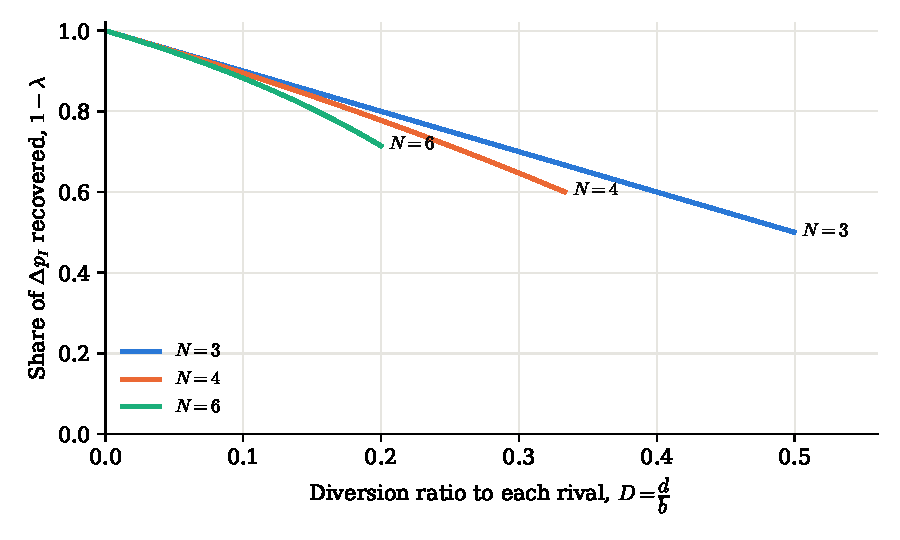
\includegraphics[width=0.78\textwidth]{figures/ch11/did_bias.pdf}
\caption{Share of the insiders' price increase recovered by a DiD estimator that uses an outsider as the control,
$1-\lambda$ from \eqref{eq:11-lambda}, against the diversion ratio to each rival $D=\frac{d}{b}$. Each curve
ends where $b=(N-1)d$. The bias is largest when the products are close substitutes, which is when the merger
matters most.}
\label{fig:11-didbias}
\end{figure}

\Cref{fig:11-didbias} shows the bias for several market sizes. Four lessons follow. First, a DiD that uses rival
brands as controls estimates a lower bound with the correct sign, which is how
\citet{AshenfelterHosken2010} and \citet{AshenfelterHoskenWeinberg2013} use it. Second, the bias grows with
diversion, so it is largest exactly when the merger has the largest effect. Third, a private-label control escapes
the bias only to the extent that store brands are distant substitutes supplied elastically. If store-brand prices
also rise, the bias has the same sign. Fourth, the rivals' price increase is itself an effect of the merger. Total
consumer harm includes it, and \cref{sec:11-dafny} shows how a study can be built on it.

\begin{remark}[General demand]\label{rem:11-didbias-general}
The linear form is not needed for the sign. Let $N=3$ and let $r(p_1,p_2)$ be the outsider's best response, with
partial derivatives $r_1,r_2>0$ (strategic complements) and $r_1+r_2<1$ (the usual stability condition). If the
symmetric insiders raise both prices by $\Delta p_I$, the mean value theorem gives
$\Delta p_O=(r_1+r_2)\big|_{\tilde p}\,\Delta p_I$ at some intermediate price vector $\tilde p$. Then
$0<\Delta p_O<\Delta p_I$. \citet{DeneckereDavidson1985} show for a broad class of demand systems that merging
firms raise prices by more than outsiders. How much outsiders respond depends on how fast elasticities change
with price \citep{CrookeEtAl1999}.
\end{remark}

\subsection{Event windows and transitory selection}\label{sec:11-retro-windows}

The \emph{event window} is the set of months used before and after the merger. It should be long enough to
capture the price change and short enough to avoid contamination by other events. \citet{AshenfelterHosken2010}
prefer a window that drops the three months before and after consummation and uses equal spans of data on the
two sides. Dropping the months near the merger avoids the question of exactly when the parties start pricing
jointly. The law prohibits joint pricing before closing, yet \citet{KimSingal1993} find that many airlines raised
fares before their mergers were consummated \citep[footnote~47]{AshenfelterHosken2008}. The symmetric design protects against a subtler
problem, which we now formalize following \citet{HeckmanRobb1985} and \citet{AshenfelterCard1985}.

Suppose that without the merger log prices follow $y_{jt}(0)=\alpha_j+\tau_t+u_{jt}$. Here $\tau_t$ is common to
all products and $u_{jt}$ is a transitory deviation. Mergers may be triggered by transitory events. A price war,
for example, depresses $u_{j t_0}$ and may push firms to merge. The General Mills purchase of the Chex brands was
announced just after a widely reported price war in ready-to-eat cereal in April 1996 \citep[p.~15]{AshenfelterHosken2008}.

\begin{definition}[Time reversibility]\label{def:11-reversible}
A stationary process $\{u_t\}$ is \emph{time reversible} if, for every $s\ge1$, the pairs $(u_{t_0+s},u_{t_0})$ and
$(u_{t_0-s},u_{t_0})$ have the same joint distribution.
\end{definition}

Every stationary Gaussian process is time reversible. Its joint distributions depend only on the autocovariance
function, and the autocovariance at lag $s$ equals the autocovariance at lag $-s$.

\begin{proposition}[Symmetric windows remove transitory selection]\label{prop:11-window}
Suppose $\{u_{jt}\}_t$ is stationary, time reversible and independent of $\alpha_j$. Suppose the event $A_j$ that
product $j$'s owner merges at $t_0$ depends only on $\alpha_j$, on $u_{jt_0}$ and on variables independent of the
process $\{u_{jt}\}$. Then for every $s\ge1$,
\begin{equation*}
\E\big[u_{j,t_0+s}-u_{j,t_0-s}\mid A_j\big]=0.
\end{equation*}
\end{proposition}

\begin{proof}
Condition first on $(\alpha_j,u_{jt_0})$ and use the law of iterated expectations:
\begin{equation*}
\E\big[u_{j,t_0+s}\mid A_j\big]=\E\Big[\E\big[u_{j,t_0+s}\mid \alpha_j,u_{jt_0}\big]\mid A_j\Big]
=\E\Big[\E\big[u_{j,t_0+s}\mid u_{jt_0}\big]\mid A_j\Big].
\end{equation*}
The second equality uses the independence of the process from $\alpha_j$ and from the other variables in $A_j$. By
time reversibility $\E[u_{j,t_0+s}\mid u_{jt_0}]=\E[u_{j,t_0-s}\mid u_{jt_0}]$. Applying the same two steps
in reverse gives $\E[u_{j,t_0-s}\mid A_j]$.
\end{proof}

The proposition implies that a comparison of month $t_0+s$ with month $t_0-s$ has no transitory selection bias.
So does any average of such comparisons over $s=k,\dots,K$. An asymmetric window does not have this property. Let
$u_{jt}$ be a Gaussian AR(1) process with coefficient $0.8$, and suppose mergers follow price wars, so that
$\E[u_{jt_0}\mid A_j]=-\mu<0$. Then $\E[u_{j,t_0\pm s}\mid A_j]=-(0.8)^{s}\mu$. Compare months 4 to 15 after
the merger with months 4 to 6 before it. The average post-merger deviation is $-0.159\mu$ and the average
pre-merger deviation is $-0.333\mu$. The estimate is biased upward by $0.174\mu$, because the recovery from the
price war is attributed to the merger. The symmetric window guards against this, at the cost of discarding data.
\citet{AshenfelterHosken2010} also report a symmetric window that keeps the months near the merger and an
asymmetric window that uses all available data. The window mattered little except for the cereal merger
\citep[p.~26]{AshenfelterHosken2008}.

Windows also determine which effects we measure. A short window captures the short-run price response. Cost
savings may take longer to reach prices. \citet{FocarelliPanetta2003} find that the price effects of the bank
mergers they study were reversed by efficiency gains after about three years. Long windows, on the other hand, mix the merger
with entry, new products and repositioning, which grow more important as time passes \citep[footnote~49]{AshenfelterHosken2008}.

\subsection{Measuring prices and drawing inferences}\label{sec:11-retro-measure}

\casehead{Unit values versus price indices} A brand is sold in several package sizes $k=1,\dots,K$ with prices per
unit $p_{kt}$ and unit sales $q_{kt}$. The \emph{unit value} or average revenue of the brand is
\begin{equation*}
P^{AR}_t=\frac{\sum_k p_{kt}q_{kt}}{\sum_k q_{kt}}=\sum_k\omega_{kt}\,p_{kt},\qquad \omega_{kt}=\frac{q_{kt}}{\sum_l q_{lt}}.
\end{equation*}
Its change between two periods decomposes as
\begin{equation*}
P^{AR}_1-P^{AR}_0=\sum_k\omega_{k0}\,(p_{k1}-p_{k0})+\sum_k(\omega_{k1}-\omega_{k0})\,p_{k1}.
\end{equation*}
The first term is a price change at fixed quantity weights. The second is a composition effect. If buyers shift
toward large packages, which are cheaper per unit, the unit value falls even when every package price rises. A
\emph{Stone price index} with fixed revenue weights $\bar w_k$ removes the composition term:
\begin{equation*}
\ln P^{S}_t=\sum_k\bar w_k\ln p_{kt},\qquad \ln P^{S}_1-\ln P^{S}_0=\sum_k\bar w_k\,(\ln p_{k1}-\ln p_{k0}).
\end{equation*}
\citet{AshenfelterHosken2010} construct five price measures for cereal, syrup and feminine hygiene products. They
are the unit value, two revenue-weighted average prices with first-year or last-year weights, and two Stone indices
with the same weights. They aggregate weekly data to months to dampen the effect of household stockpiling during sales
\citep{HendelNevo2006}. Scanner data also record retail prices. A merger of manufacturers changes wholesale
prices, and retail prices change by the retailers' pass-through of the wholesale change.

\casehead{Clustered errors} In \eqref{eq:11-ah-price} the regressor $\mathit{Post}_t$ takes the same value for
every product and region in a month. Common monthly shocks then make the errors of a month correlated, and
conventional standard errors are too small \citep{Moulton1987}.

\begin{lemma}[Moulton factor]\label{lem:11-moulton}
Let $y_{it}=\beta_0+\beta x_t+e_{it}$ for $i=1,\dots,m$ observations in each of $T$ months, with
$e_{it}=v_t+w_{it}$, where $v_t$ and $w_{it}$ are independent with mean zero and variances $\sigma_v^2$ and
$\sigma_w^2$. Let $\rho_e=\frac{\sigma_v^2}{\sigma_v^2+\sigma_w^2}$. Then the variance of the OLS estimator
$\hat\beta$ is $1+(m-1)\rho_e$ times the conventional formula that treats the errors as independent.
\end{lemma}

\Cref{lem:11-moulton} is the special case of \cref{prop:A-moulton} with months as clusters of size $m$. The error
components make the errors homoskedastic with variance $\sigma_v^2+\sigma_w^2$, independent across months and
equicorrelated within a month with correlation $\rho_e$. The regressor is constant within a month, so its
intra-cluster correlation is $\rho_x=1$. Then \eqref{eq:A-moulton} gives the factor $1+(m-1)\rho_e$.

With 64 regions and an intra-month correlation of only $0.1$, the factor is $7.3$, and the correct standard error
is $2.7$ times the conventional one. \citet{AshenfelterHosken2010} cluster by month. Clustering by month also
requires enough months, and serial correlation across months is a further concern in DiD designs
\citep{BertrandDufloMullainathan2004}.

\subsection{Which mergers can we study? Selection by the agencies}\label{sec:11-retro-select}

The agencies screen proposed mergers and block or modify those they expect to raise prices. As
\cref{sec:11-review} showed, about 97\% of the mergers filed from 1991 to 2004 went ahead without a full
investigation, and most of the rest were modified, abandoned or blocked. Retrospective samples therefore contain
only cleared mergers. A simple model shows what such samples can reveal.

\begin{assumption}[Screening on a noisy signal]\label{ass:11-screen}
Merger $m$ has a true price effect $\Delta_m$. The agency observes a signal $S_m=\Delta_m+\eta_m$ and clears the
merger if $S_m\le\bar s$. The pair $(\Delta_m,\eta_m)$ is jointly normal and independent across mergers, with
$\Delta_m$ of mean $\mu_\Delta$ and variance $V_\Delta>0$, and $\eta_m$ of mean zero and variance $V_\eta$,
independent of $\Delta_m$.
\end{assumption}

\begin{proposition}[What cleared mergers reveal]\label{prop:11-select}
Under \cref{ass:11-screen},
\begin{equation*}
\E[\Delta_m\mid S_m\le\bar s]\ \le\ \E[\Delta_m\mid S_m=\bar s]\ \le\ \E[\Delta_m\mid S_m>\bar s],
\end{equation*}
and $\E[\Delta_m\mid S_m\le\bar s]\le\mu_\Delta$, the average effect without enforcement.
\end{proposition}

\begin{proof}
Joint normality gives the linear conditional expectation
\begin{equation*}
\E[\Delta_m\mid S_m=s]=\mu_\Delta+k\,(s-\mu_\Delta),\qquad k=\frac{V_\Delta}{V_\Delta+V_\eta}\in(0,1],
\end{equation*}
which is increasing in $s$. Averaging an increasing function over $s\le\bar s$ gives at most its value at $\bar
s$, and averaging over $s>\bar s$ gives at least that value. Finally, $\mu_\Delta$ is a weighted average of the
cleared and blocked means, so it lies between them.
\end{proof}

A random sample of cleared mergers therefore gives a lower bound on the price effect of a typical merger in a
world without enforcement \citep{Carlton2009}. That bound says little about policy, because most proposed
mergers raise no competitive concern. The informative object is the effect of the \emph{marginal merger},
$\E[\Delta_m\mid S_m=\bar s]$. If it is positive, enforcement under a consumer-welfare standard is too lenient at
the margin. If it is negative, enforcement is too strict \citep{AshenfelterHoskenWeinberg2013}. Both studies below
target the margin. \citet{AshenfelterHosken2010} pick cleared mergers that look most problematic from public
information. Their estimates therefore bound from above the effects of other cleared mergers and from below the
effects of blocked ones. \citet{AshenfelterHoskenWeinberg2013} study a merger that was nearly challenged. Two caveats
apply. Researchers see public concentration measures, which are a noisy proxy for the agency's signal. And
samples are also selected by data availability, which favors consumer products and formerly regulated
industries such as airlines, banking and hospitals.

\subsection{Stock-market event studies}\label{sec:11-retro-event}

Before scanner data, retrospectives used stock prices. The method of abnormal returns is developed in
\cref{sec:A-eventstudy}, and \cref{sec:09-wc-method} applies it to airline entry. Its application to mergers, due to \citet{Eckbo1983} and \citet{Stillman1983}, looks at
the merging firms' \emph{rivals}. A merger that raises market power, through unilateral or coordinated effects,
raises rivals' profits. A merger that makes the merged firm a more efficient and tougher competitor lowers them.
News that raises the chance of the merger (the announcement) and news that lowers it (an antitrust complaint)
therefore move rivals' values in opposite directions under each hypothesis. \Cref{tab:11-eventpred} lists the
predictions.

\begin{table}[htbp]
\centering
\caption{Predicted abnormal returns of rival firms}
\label{tab:11-eventpred}
\footnotesize
\begin{tabular}{@{}lcc@{}}
\toprule
Hypothesis & Merger announcement & Antitrust complaint \\
\midrule
Market power (higher post-merger prices) & $+$ & $-$ \\
Efficiency (merged firm a tougher rival) & $-$ & $+$ \\
Information (merger reveals industry-wide gains) & $+$ & $0$ \\
\bottomrule
\end{tabular}

\smallskip
\begin{minipage}{0.85\linewidth}
\footnotesize Notes: Signs of rivals' cumulative abnormal returns. Under the information hypothesis the
announcement reveals profitable opportunities, such as scale economies or the value of rivals as future targets,
that a complaint against one merger does not withdraw.
\end{minipage}
\end{table}

\citet[p.~269]{Eckbo1983} studies the rivals of 65 challenged horizontal mergers. On average they earned an
abnormal return of 2.45 percent over the 31 days around the merger proposal, more than three standard deviations
from zero. Over the 31 days around the antitrust complaint their average return was 1.78 percent, about one standard
deviation from zero, so they did not lose. Eckbo concludes that the data generally reject the collusion hypothesis
(p.~242). He reads the rivals' gains at the proposal as news of cost savings that they can also achieve. He calls
this the productive efficiency hypothesis, which corresponds to the information row of \cref{tab:11-eventpred}.
\citet[p.~240]{Stillman1983} studies the rivals of 11
challenged horizontal mergers attempted between 1964 and 1972. Only in the merger of Sterling Drug and Lehn and Fink
did their returns broadly follow the market-power pattern. In nine of the 11 mergers the rivals showed no abnormal
returns of any kind.
These designs have known limits. Rival returns mix the three hypotheses. News may be anticipated, so the window
captures only part of it. Rivals are often diversified firms, and the affected market can be a small part of
their value. Many relevant rivals are not publicly traded. \citet{Woolley1989} applies the method to 29
merger-related events in hospital chains between 1969 and 1985. \citet{VitaSchumann1991} criticize his choice of
events and rivals and note that listed chains own a small share of hospitals (\citealp[p.~11]{Dafny2005}).
\citet{McAfeeWilliams1988} study the 1979 acquisition of Kalvar by Xidex, two producers of duplicate microfilm. The FTC
challenged the merger in September 1980 (p.~201). McAfee and Williams cite \citet{BartonSherman1984}, who find that
the ratio of vesicular to diazo prices paid by the federal government rose about 25 percent after the merger
\citep[p.~200]{McAfeeWilliams1988}.
An event study of the rivals' returns nevertheless shows no evidence of harm (pp.~202--203).
\citet[p.~231, n.~137]{AskerNocke2021} reach a similar verdict on the literature that runs from \citet{Eckbo1983}
and \citet{Stillman1983} to \citet{DusoNevenRoller2007}. Most authors in it are cautious about what an event study
reveals about the competitive effects of a particular merger. In the words of \citet{KaplowShapiro2007}, an event
study ``measures the expectations of investors about merger effects, not the actual effects of mergers.'' The method
has worked best for patterns across large samples of mergers, as in \citet{DusoNevenRoller2007}. For these reasons
modern retrospectives measure prices directly.

\subsection{Five consumer-product mergers: Ashenfelter and Hosken (2010)}\label{sec:11-ah}

\casehead{Question and design} \citet{AshenfelterHosken2010} ask whether the mergers that the agencies let through
raised consumer prices.\footnote{We use the NBER working-paper version \citep{AshenfelterHosken2008}. Table
numbers and page references follow it.} Their design follows \cref{prop:11-select}. They search the Merger
Yearbook for consummated mergers in consumer-product industries between 1997 and 1999 whose parties sold
substitutes in concentrated markets. The period is fixed by the data, because the vendor sold scanner data only
for the previous five years. Three of the five selected mergers went through without government action:
Procter and Gamble's purchase of Tambrands, Aurora Foods' purchase of Kraft's Log Cabin syrup, and Pennzoil's
purchase of Quaker State. Two were modified by the FTC: General Mills' purchase of Ralcorp's branded cereals and
the merger of Guinness and Grand Metropolitan into Diageo. All five produced highly concentrated markets (HHI above
1,800) with HHI increases above 100 points, the 1992 Guidelines' presumption of harm.

The authors argue that these mergers sit near the enforcement margin. In the FTC's investigations of fiscal years
1996--2003, 46\% of markets had post-merger HHI below 3,000 and 51\% had increases below 800 points. All five
mergers have post-merger HHIs below 3,000 and HHI changes between 200 and 1,000 points, so they sit near the median
of the investigated markets (p.~12). The FTC acted in 25\% of investigated markets with post-merger HHI below 2,500
(four of the five mergers) and in 44\% of markets with increases below 800 (pp.~11--12).

\casehead{The five mergers} Procter and Gamble bought Tambrands for \$1.85 billion in July 1997, adding the leading
tampon (Tampax) to the leading sanitary pad (Always). The Justice Department reviewed the deal and took no
action. Guinness and Grand Metropolitan combined their spirits portfolios in a transaction valued at about \$36
billion. The FTC found harm in premium scotch and premium gin and required the sale of the Bombay gins and Dewar's
scotch to Bacardi for \$1.9 billion. Pennzoil bought Quaker State for \$1 billion in December 1998, combining two
of the five premium motor-oil brands. General Mills bought the Chex cereals for \$570 million in January 1997.
Ralcorp kept its private-label business, the largest in the country, and the FTC's modifications let Ralcorp make
private-label Chex at once. Aurora, owner of Mrs.\ Butterworth's, bought Log Cabin for \$222 million in July 1997,
joining two of the three major syrup brands (pp.~12--16). \Cref{tab:11-ah} reports shares and concentration,
and \cref{tab:11-ahhhi} in \cref{sec:11-hhi} checked the reported changes in concentration against $2s_As_B$.

\begin{table}[htbp]
\centering
\caption{Five consumer-product mergers: concentration and aggregate price effects}
\label{tab:11-ah}
\footnotesize
\begin{tabular}{@{}lcccccc@{}}
\toprule
& & & & & \multicolumn{2}{c}{Aggregate price effect} \\
\cmidrule(l){6-7}
Transaction (industry) & Shares (\%) & HHI & $\Delta$HHI & & Private label & Branded \\
\midrule
General Mills / Ralcorp (cereal) & 28, 4 & 2,357 & 238 & & 0.032 & 0.057 \\
 & & & & & (0.005) & (0.005) \\
Pennzoil / Quaker State (motor oil) & 29, 9 & 2,189 & 517 & & 0.052 & 0.014 \\
 & & & & & (0.013) & (0.011) \\
P\&G / Tambrands (feminine protection) & 25, 19 & 2,815 & 959 & & 0.070 & 0.023 \\
 & & & & & (0.008) & (0.007) \\
Aurora / Log Cabin (pancake syrup) & 15, 19 & 1,990 & 589 & & 0.004 & 0.012 \\
 & & & & & (0.011) & (0.005) \\
Guinness / Grand Met (liquor), overall & 21, 22 & 2,026 & 935 & & 0.027 & $-0.010$ \\
 & & & & & (0.003) & (0.003) \\
\quad gin & & & & & 0.022 & $-0.021$ \\
 & & & & & (0.005) & (0.003) \\
\quad scotch & & & & & 0.071 & 0.031 \\
 & & & & & (0.006) & (0.002) \\
\quad vodka & & & & & 0.011 & $-0.021$ \\
 & & & & & (0.003) & (0.005) \\
\bottomrule
\end{tabular}

\smallskip
\begin{minipage}{0.97\linewidth}
\footnotesize Notes: Shares are pre-merger revenue shares of the acquirer and the target, in that order (for syrup,
Aurora then Philip Morris's Log Cabin). HHI is the post-merger HHI and $\Delta$HHI its change, from pre-merger
revenue data, with private labels treated as one participant. Price effects are the revenue-weighted averages
\eqref{eq:11-ah-agg} of the product-level estimates of $\beta_2$ in \eqref{eq:11-ah-price}, using the private-label
or the branded control group. Standard errors in parentheses assume zero covariances among the components. The data come from IRI's food channel (64 regions) for
cereal, feminine protection and syrup, its mass-merchandiser channel (10 regions) for motor oil, and its drug-store
channel (5 regions) for liquor. Source: \citet{AshenfelterHosken2008}, Tables 2 and 13.
\end{minipage}
\end{table}

\casehead{Data} The data are weekly revenue and unit sales by Universal Product Code (UPC), purchased from
Information Resources Inc.\ (IRI) and aggregated to months. IRI projects sales for each channel and metropolitan
area from a sample of stores. The authors choose for each merger the channel that best represents consumer
purchases. Food products use the food channel in 64 InfoScan markets. Motor oil uses the mass-merchandiser channel
in 10 markets, because consumers who change their own oil buy it there. Liquor uses the only available source, a
drug-store sample with complete data for five markets in three states. The markets are San Francisco, San Diego,
Los Angeles, Chicago and Phoenix, which limits external validity (pp.~16--18). Motor oil is priced as revenue per quart for
each brand and weight. Spirits are priced separately for the 750 ml and 1.75 litre bottles. The other categories
use the five price measures of \cref{sec:11-retro-measure}.

\casehead{Estimation} The price equation \eqref{eq:11-ah-price} is fitted by OLS separately for each merging
product, with standard errors clustered by month. The preferred specification uses the unit value, the symmetric
window that drops three months on each side, and one of two control groups. The \emph{private-label control} uses
the store brands closest to each merging product. These are private-label motor oil, feminine hygiene products and
maple-flavored syrup, private-label gin, scotch and vodka for the spirits, and private-label cereals in the same
IRI segments for cereal. The \emph{branded control} uses close branded substitutes, such as the three other premium motor oils
(Havoline, Valvoline and Castrol). The authors treat the branded estimates mainly as a specification check, for the
reason given in \cref{prop:11-didbias} (pp.~23--24). They also report regressions with no control group.

\casehead{Results} \Cref{tab:11-ah} gives the aggregate effects (Table 13). With the private-label control, four of
the five mergers raised prices by roughly 3\% to 7\%. The estimates are 3.2 log points for General Mills and Chex,
5.2 for Pennzoil and Quaker State, 7.0 for Procter and Gamble and Tambrands, and 2.7 for Diageo. The syrup merger had no
detectable effect (0.4). The branded control gives larger effects for cereal and syrup and smaller ones for the
other three. The spirits merger illustrates the role of the control group. Scotch prices rose under both controls
(7.1 and 3.1 log points), while gin and vodka rose relative to private labels and fell relative to branded
rivals.

The product-level estimates show that the merged firms did not raise all prices together. \Cref{tab:11-ah-pqs}
reproduces Table 3 for motor oil. Relative to private labels, Quaker State rose 8.1 log points and Quaker State
Deluxe 6.1, while the much larger Pennzoil brand rose 3.9. In Table 3, Quaker State's increase ranks first among
the 12 products compared, its own and the 11 branded controls. The text instead describes it as larger than all but
one control brand (p.~28). Market shares moved accordingly. Quaker State lost 1.31 points of revenue share, 13.6\%
of its pre-merger share, while Pennzoil gained 4.22 points. Because Pennzoil's gain exceeded Quaker State's loss,
it grew at the expense of rivals as well. The authors read this as a strategy of raising the price to customers
loyal to Quaker State while holding the price of the larger brand (p.~29).

\begin{table}[htbp]
\centering
\caption{Pennzoil and Quaker State: product-level price and share effects}
\label{tab:11-ah-pqs}
\footnotesize
\begin{tabular}{@{}lcccccc@{}}
\toprule
& \multicolumn{2}{c}{Price effect $\hat\beta_2$} & \multicolumn{2}{c}{Rank in control group} &
\multicolumn{2}{c}{Change in revenue share} \\
\cmidrule(lr){2-3}\cmidrule(lr){4-5}\cmidrule(l){6-7}
Product & Branded & Private label & Branded & Private label & Points & Percent \\
\midrule
Pennzoil & 0.004 & 0.039 & 8/12 & 1/2 & 4.22 & 18.47 \\
 & (0.015) & (0.019) & & & (0.83) & \\
Quaker State & 0.035 & 0.081 & 1/12 & 1/2 & $-1.31$ & $-13.58$ \\
 & (0.016) & (0.015) & & & (0.47) & \\
Quaker State Deluxe & 0.021 & 0.061 & 4/12 & 1/2 & $-0.16$ & $-5.95$ \\
 & (0.021) & (0.022) & & & (0.13) & \\
\bottomrule
\end{tabular}

\smallskip
\begin{minipage}{0.95\linewidth}
\footnotesize Notes: Standard errors in parentheses. The rank orders the product's estimated price change among
the control products in descending order: 8/12 means that seven control products had larger increases. Quantity
shares move similarly ($+4.46$, $-1.32$ and $-0.13$ points). Monthly data from 10 regions of IRI's
mass-merchandiser channel, January 1997 to December 2000, excluding October 1998 to March 1999. An observation is
a product, city and month. The regressions have about 9,000 (branded control) and 2,000 (private-label control)
observations. Source: \citet{AshenfelterHosken2008}, Table 3.
\end{minipage}
\end{table}

The other mergers show the same selectivity (Tables 5, 7, 9 and 11). After buying Tambrands, Procter and Gamble
raised the prices of Always liners and pads by 8.0 and 7.8 log points relative to store brands, and Tampax by
5.8.
Relative to branded products the liner and pad increases were 6.1 and 4.5, and Tampax fell by 0.9. A later study
of the same merger, \citet{Weinberg2011}, reports increases of 8 percent for Always pads and 5 percent for Tampax
relative to private label \citep[p.~262]{AskerNocke2021}. General
Mills left the Chex prices almost unchanged (at most 0.8 log points under either control) and raised the prices
of its own Cheerios and Wheaties brands. Cheerios rose 4.4 log points relative to store brands and 4.6 relative
to branded cereals. Every scotch product rose relative to its private-label control, by 5.5 to 9.8 log points.
For syrup, Log Cabin's 2.8 log point rise relative to branded syrups was not robust, and Mrs.\ Butterworth's prices
did not change.

\casehead{Robustness} For each merger, a summary table pools the estimates across windows, price measures and
control groups (Tables 4, 6, 8, 10 and 12). For motor oil, all 18 estimates are positive. All nine private-label
estimates have $t$-statistics above two, against three of the nine branded estimates. For feminine protection,
92\% of the private-label estimates and 78\% of the branded ones are positive. About 90\% of the cereal estimates
are positive, and none of the negative ones is below $-1\%$. For syrup, about two thirds fall between $-1\%$ and
$+1\%$. The choice of window mattered little except for cereal. The price measure left the signs unchanged and
changed the magnitudes. With weekly data the cereal estimates depended heavily on the price measure, which points to
stockpiling and package substitution (pp.~26--32). Regressions with no control group also show price increases
after virtually every merger (Appendix Tables 3--7). For example, the no-control estimates for Quaker State and
Always pads are 0.061 (0.016) and 0.053 (0.003).

\casehead{Comparison with a merger simulation} The General Mills and Chex merger had been simulated by
\citet{Nevo2000b} with a random-coefficients demand model (\cref{sec:11-simulation}). As cited by Ashenfelter and
Hosken, the published simulation predicts increases before efficiencies of 12.2\% for Chex, 1.1\% for Cheerios,
0.8\% for Honey Nut Cheerios and 0.1\% for Wheaties (p.~32). The retrospective finds the opposite pattern: little
change for Chex and increases for the General Mills brands. Possible reasons include the different data
(quarterly data for 1988--1992 in the simulation), new product introductions, and the demand specification. The
consent decree's provision for private-label Chex may also have restrained Chex pricing, an entry threat that a
simulation with a fixed set of products cannot represent (footnote 60).

\casehead{Interpretation and limitations} The best estimate of the price effect of mergers near the enforcement
margin is positive and modest. This finding cuts against both camps in the enforcement debate. Advocates of less
intervention expect the marginal merger to lower prices through efficiencies, and advocates of more intervention
expect large increases (p.~35). The authors list three limitations themselves (p.~36). Consumer-product mergers are a
small part of all mergers: 20 percent of the 8,013 filings in 1997 and 1998 shared the studied firms' two-digit
industry codes. The design cannot capture longer-run efficiency effects or new products. Finally, the study examines
only one kind of enforcement error, the failure to block harmful mergers, and leaves aside the blocking or
deterrence of benign ones. Several further points deserve attention. The selection rests on public concentration measures, which
may misjudge which mergers the agencies found marginal. The private-label control may itself be a substitute,
especially in cereal, where Ralcorp kept a large store-brand business. The aggregate standard errors ignore
covariances, as shown after \eqref{eq:11-ah-agg}. Retail scanner prices measure the merger's effect after
retailers' pass-through. Finally, the results vary across products within a merger, so several products and
specifications are tested for each merger, and some significant estimates will arise by chance.

\casehead{Contribution} The paper turned merger retrospectives into a program-evaluation exercise with explicit
attention to control groups, windows, price measurement and the selection of mergers. It shows that a cleared
merger's effect can be concentrated on a few products, and it supplied the retrospective benchmarks later used to
grade merger simulations.

\subsection{A nearly blocked merger of appliance makers: Ashenfelter, Hosken and Weinberg (2013)}\label{sec:11-maytag}

\casehead{Question} \citet{AshenfelterHoskenWeinberg2013} estimate the price effects of Whirlpool's acquisition of
Maytag.\footnote{We use the NBER working-paper version \citep{AshenfelterHoskenWeinberg2011}. Table numbers
follow it and may differ from the published article.} The merger is a natural candidate for the marginal merger
of \cref{prop:11-select}. Commentators argued that the Justice Department would have challenged it a decade
earlier, and the decision not to act came to symbolize lenient enforcement \citep{BakerShapiro2008}.

\casehead{Background} In mid-2005 a group of private investors agreed to buy Maytag for \$1.13 billion. The Haier
Group, a Chinese appliance maker with little presence in the United States, then offered \$1.3 billion. Whirlpool,
the largest United States manufacturer, offered \$1.4 billion on July 17, and Haier withdrew three days later.
Whirlpool bought Maytag for \$1.79 billion on March 30, 2006, after a long Justice Department investigation. The
merger reduced the major appliance manufacturers from four (Whirlpool, Maytag, GE and Electrolux) to three. The
Justice Department's closing statement of March 29, 2006, focused on washers and dryers and gave three reasons for
not acting. GE and Electrolux had excess capacity, and the recent entrants LG and Samsung could expand imports.
Large retailers had alternatives to resist price increases. The parties had substantiated large cost savings
(printed pp.~4--6 and 21).

\casehead{Market structure} \Cref{tab:11-maytag} reproduces the pre-merger revenue shares. Whirlpool was the
largest firm in dishwashers, dryers, refrigerators and washers, with 39\% to 49\% of revenue, and Maytag held 9\%
to 17\%. The increase in the HHI matches $2s_Ws_M$ in every category up to rounding of the
shares, within three points. In dryers, for example, $2\times48.8\times16.6=1{,}620$. The parties overlapped less in
cooktops, freezers, ovens and ranges. Neither had more than 1 percent of freezer revenue, Maytag held 5 to 10 percent
of the other three, and the implied HHI changes were 256 to 416 points.
These four categories serve as comparison groups, restricted to brands not made by Whirlpool or Maytag.

\begin{table}[htbp]
\centering
\caption{Whirlpool and Maytag: pre-merger revenue shares and concentration}
\label{tab:11-maytag}
\footnotesize
\begin{tabular}{@{}lccccc@{}}
\toprule
Category & Whirlpool & Maytag & Largest rivals & HHI & $\Delta$HHI \\
\midrule
\multicolumn{6}{@{}l}{\textit{Treated categories}} \\
Dishwashers & 38.6 & 11.4 & Electrolux 25.1, GE 12.5 & 2,453 & 880 \\
Clothes dryers & 48.8 & 16.6 & GE 12.2, LG 9.6, Electrolux 8.9 & 2,983 & 1,620 \\
Refrigerators & 41.8 & 9.2 & Electrolux 24.1, GE 10.9 & 2,595 & 770 \\
Clothes washers & 44.0 & 16.8 & Electrolux 13.8, GE 10.5, LG 10.2 & 2,632 & 1,478 \\
\addlinespace
\multicolumn{6}{@{}l}{\textit{Comparison categories}} \\
Cooktops & 22.0 & 9.5 & GE 20.8, Electrolux 19.1 & 1,571 & 416 \\
Freezers & $<1$ & $<1$ & Electrolux 81.3, Haier 12.8 & 6,789 & 0 \\
Ovens & 32.5 & 6.3 & GE 23.1, Electrolux 10.5 & 1,929 & 412 \\
Ranges & 24.7 & 5.2 & Electrolux 37.6, GE 25.3 & 2,703 & 256 \\
\bottomrule
\end{tabular}

\smallskip
\begin{minipage}{0.95\linewidth}
\footnotesize Notes: Revenue shares in percent from NPD data before the merger. HHI is the pre-merger HHI as
labelled in the source. Neither party had more than 1\% of freezer revenue before the merger. Kenmore, sold by
Sears and partly made by Whirlpool, is not in the data. Source: \citet{AshenfelterHoskenWeinberg2011}, Tables 1
and 2.
\end{minipage}
\end{table}

\casehead{Data} The NPD Group supplied national monthly unit sales and revenue for each appliance model, identified
by its stock-keeping unit (SKU), from January 2005 to September 2008. More than 14,000 SKUs enter during the
period, and observed characteristics explain 85\% to 95\% of the variation in prices. Two features of the industry
shape the design. First, most appliances have a life cycle of about a year. The authors estimate age profiles
separately for each category,
\begin{align}
\ln p_{jt}&=\alpha_j+\sum_{k=2}^{25}\theta_k\,\mathit{Age}_{kjt}+\sum_{l=2}^{43}\delta_l\,\mathit{Month}_{lt}+e_{jt},\label{eq:11-ahw-age}\\
\ln q_{jt}&=\psi_j+\sum_{k=3}^{25}\lambda_k\,\mathit{Age}_{kjt}+\sum_{l=3}^{43}\gamma_l\,\mathit{Month}_{lt}+u_{jt},\nonumber
\end{align}
where $\mathit{Age}_{kjt}$ indicates that model $j$ is $k$ months old.\footnote{In this subsection $\theta_k$,
$\delta_l$, $\psi_j$, $\lambda_k$ and $\gamma_l$ are regression coefficients with no relation to their meanings
elsewhere in the book.} Prices of washers, dryers, dishwashers, refrigerators, freezers and ranges typically fall by more
than 10\% after a year, and monthly sales fall by about half. Ovens and cooktops show no such decline. The analysis
therefore uses each model's first year only and controls for age by category. Second, many SKUs sell very few
units. The sample keeps models with at least 1,000 units in their first 13 months (100 for freezers, ovens and
cooktops). The retained models account for 90\% to 99\% of sales in the large categories (printed pp.~6--9).

\casehead{Estimating equations} The baseline specification, fitted by OLS separately for each treated and
comparison pair of categories, is
\begin{multline}\label{eq:11-ahw-fe}
\ln p_{jt}=\beta_1\,\mathit{Maytag}_j\,\mathit{Post}_t+\beta_2\,\mathit{Whirlpool}_j\,\mathit{Post}_t\\
+\sum_{k=3}^{13}\theta_k^{T}\mathit{Age}^{T}_{kjt}+\sum_{k=3}^{13}\theta_k^{C}\mathit{Age}^{C}_{kjt}+\sum_{l=2}^{43}\delta_l\,\mathit{Month}_{lt}+\alpha_j+e_{jt}.
\end{multline}
It has separate age profiles for the treated ($T$) and comparison ($C$) categories, month effects and SKU fixed
effects $\alpha_j$. The SKU fixed effects have a cost. The interactions are collinear with $\alpha_j$ for any model
sold only before or only after the merger. Equation \eqref{eq:11-ahw-fe} therefore identifies the effects only from
models sold on both sides of the merger date. With one-year life cycles, these are old models, and the merged firm may have
treated them differently from new ones. The authors therefore replace the fixed effects with observed
characteristics and brand dummies, such as a stainless-steel indicator, size, capacity and cycles:
\begin{multline}\label{eq:11-ahw-char}
\ln p_{jt}=x^{T}_{j}\beta^{T}+x^{C}_{j}\beta^{C}+\sum_{l=2}^{43}\delta^{C}_l\,\mathit{Month}_{lt}+\beta_1\,\mathit{Maytag}_j\,\mathit{Post}_t+\beta_2\,\mathit{Whirlpool}_j\,\mathit{Post}_t\\
+\sum_{k=3}^{13}\theta_k^{T}\mathit{Age}^{T}_{kjt}+\sum_{k=3}^{13}\theta_k^{C}\mathit{Age}^{C}_{kjt}+e_{jt}.
\end{multline}
Here $x^T_j$ is non-zero only for the parties' models and $x^C_j$ only for comparison models. Standard errors
are clustered by SKU. The check on this substitution is direct. On models sold both before and after the merger,
the two specifications give estimates within 0.2 percentage points of each other against cooktops and ranges.
Against cooktops, for instance, the Whirlpool dishwasher effect is 0.0432 with fixed effects and 0.0415 with
characteristics (Appendix Table 1). The gaps reach 0.7 points against ovens and 1 to 2 points against freezers, well
within one standard error (Appendix Tables 2--4).

The main specification splits each interaction by whether the model was introduced before (Old) or after (New)
the merger, which adds 35\% to 57\% to the sample. A within-category variant compares the parties' models with
rivals' models in the same category,
\begin{multline}\label{eq:11-ahw-rival}
\ln p_{jt}=x_j\beta+\sum_{k}\theta_k\,\mathit{Age}_{kjt}+\sum_{l}\delta_l\,\mathit{Month}_{lt}
+\beta_1\,\mathit{Maytag}_j\mathit{Post}_t\mathit{Old}_j+\beta_2\,\mathit{Whirlpool}_j\mathit{Post}_t\mathit{Old}_j\\
+\beta_3\,\mathit{Maytag}_j\mathit{Post}_t\mathit{New}_j+\beta_4\,\mathit{Whirlpool}_j\mathit{Post}_t\mathit{New}_j+e_{jt}.
\end{multline}
By \cref{prop:11-didbias}, the rival comparison is biased toward zero if rivals' models are substitutes.
Finally, product variety is measured by the number of SKUs selling at least 100 units a month,
\begin{equation}\label{eq:11-ahw-sku}
\ln\mathit{SKU}_{ft}=a+b\,\mathit{WM}_f+g\,\mathit{Post}_t+\delta^{V}\,\mathit{WM}_f\,\mathit{Post}_t+e_{ft},
\end{equation}
where $f$ is either the merged firm ($\mathit{WM}_f=1$) or all rivals together. The coefficient $\delta^V$ is the
proportional change in the merged firm's product count relative to rivals.

\casehead{Identification} The comparison categories identify the counterfactual price path. The design assumes that
cooktops, freezers, ovens and ranges made by other firms would have followed the same age- and
characteristic-adjusted price trend as the treated categories. All are durable goods bought with new homes and
remodeling, so they share much of the demand shock from the housing market. The data are national, so there is no
geographic variation. Identification rests entirely on comparisons across categories and, in
\eqref{eq:11-ahw-rival}, across firms within a category.

\begin{figure}[htbp]
\centering
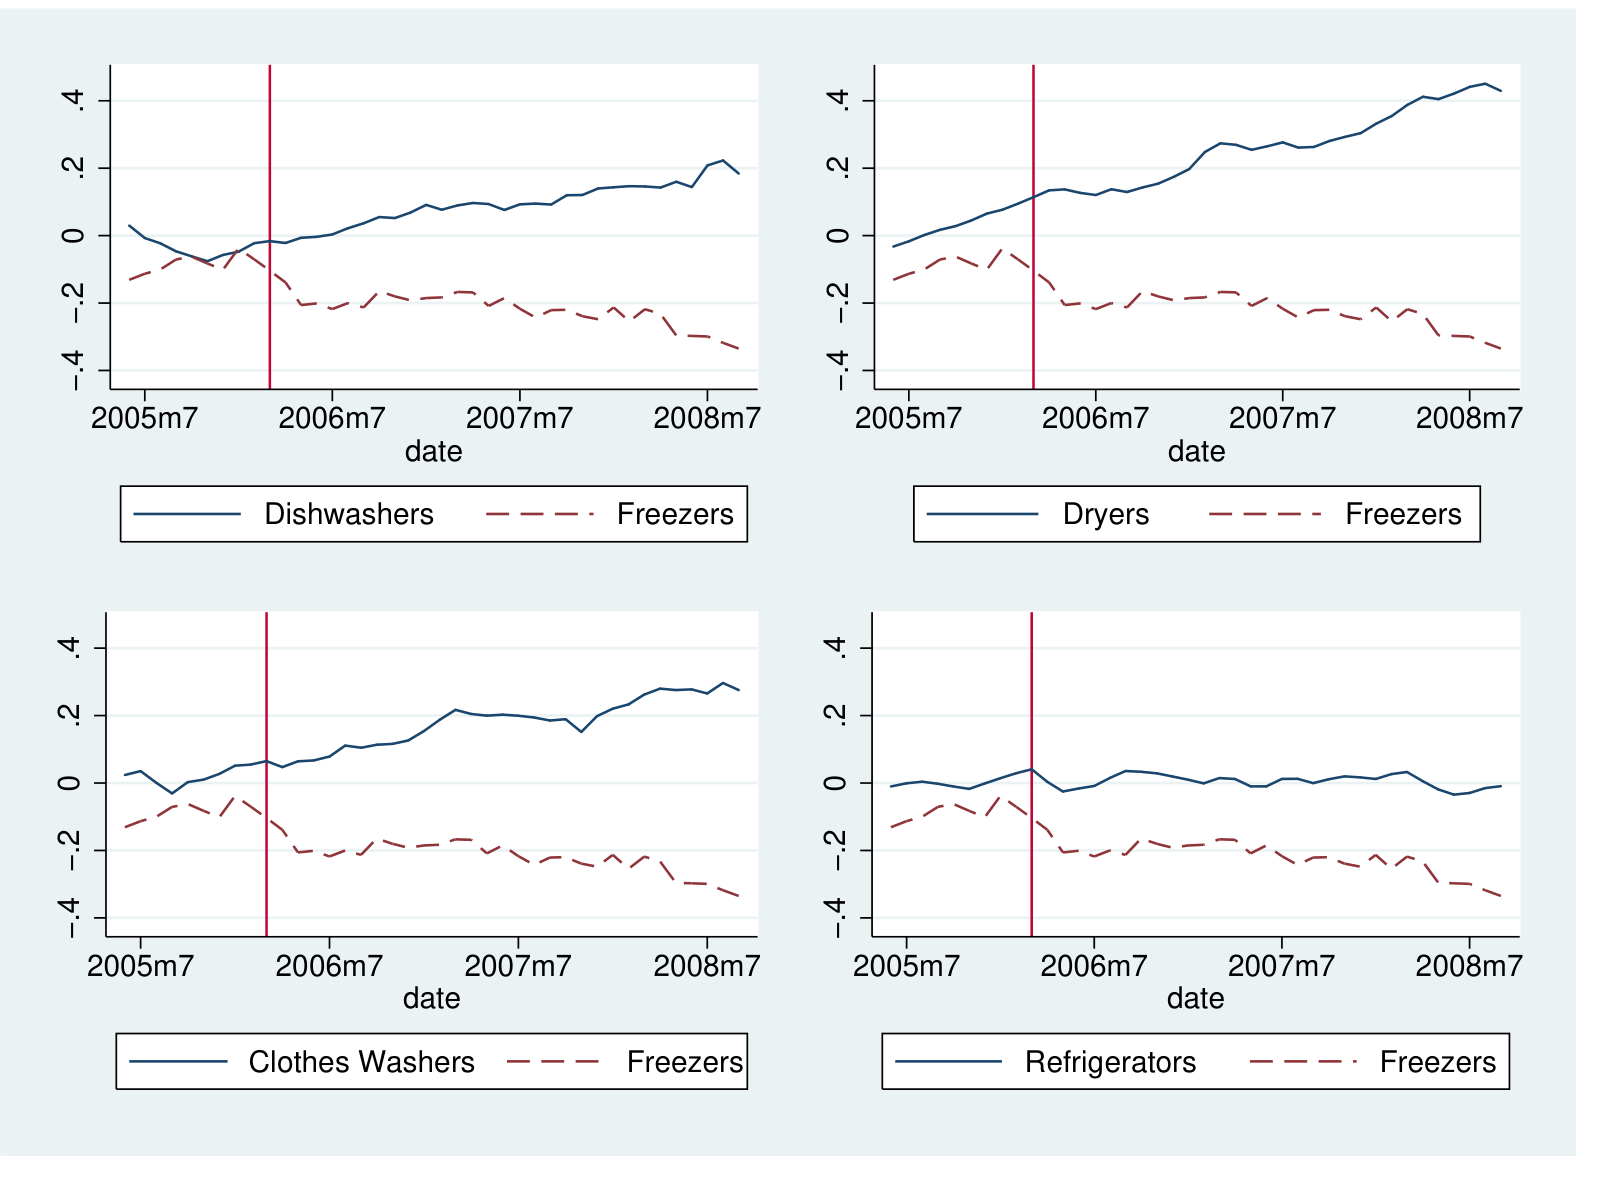
\includegraphics[width=0.86\textwidth]{figures/ch11/ahw_fig5.png}
\caption{Average log prices of Whirlpool and Maytag appliances (solid) and of freezers (dashed), adjusted for
product characteristics and age, May 2005 to September 2008. The vertical line marks consummation (March 30,
2006). Dishwasher, dryer and washer prices rise relative to freezers after the merger. Refrigerator prices do not.
The averages pool old and new models. The vintage-split regressions of \cref{tab:11-maytag-res} find no increase for
new washers. Source: \citet{AshenfelterHoskenWeinberg2011}, Figure 5.}
\label{fig:11-maytag}
\end{figure}

\casehead{Results} \Cref{fig:11-maytag} plots adjusted prices against freezers. \Cref{tab:11-maytag-res} reproduces
the regression estimates for the four treated categories against each comparison category (Tables 3 to 6) and
against rivals in the same category (Table 7). The clearest effects are for models introduced after the merger.
New Whirlpool dryers rose by 13.3 to 17.1 log points relative to the comparison categories, all significant. New
Maytag dishwashers rose by 4.8 to 7.4 log points, all significant at 5\%. New Whirlpool refrigerators rose by 1.9 to
3.9 log points, significant except against freezers. The authors give this result little weight. They describe ``a
small price increase, 2-4\%, for Whirlpool refrigerators'' that is ``imprecisely estimated and not as robust as the
findings for clothes dryers or dishwashers'' (printed pp.~15--16). The within-category estimate is only 0.008
(0.009), and their abstract concludes that there were ``no price effects for refrigerators or clothes washers''
(PDF p.~1). \citet[p.~262]{AskerNocke2021} quote the same sentence from the published abstract. Washers show no
increase. New Whirlpool washers in fact fell
by 1.5 to 4.1 log points. Estimates for models introduced before the merger depend on the comparison category.
They tend to be positive against cooktops and freezers and smaller or negative against ovens and ranges. The
within-category comparison tells the same story: new Maytag dishwashers rose 8.2 log points and new Whirlpool
dryers 7.3 log points relative to rivals' new models.

\begin{table}[htbp]
\centering
\caption{Whirlpool and Maytag: price effects by category, model vintage and comparison group}
\label{tab:11-maytag-res}
\footnotesize
\begin{tabular}{@{}lccccc@{}}
\toprule
& \multicolumn{4}{c}{Comparison category, \eqref{eq:11-ahw-char} split by vintage} & Rivals, \eqref{eq:11-ahw-rival} \\
\cmidrule(lr){2-5}\cmidrule(l){6-6}
Post-merger $\times$ & Cooktops & Freezers & Ovens & Ranges & Same category \\
\midrule
\multicolumn{6}{@{}l}{\textit{Clothes dryers}} \\
Old $\times$ Whirlpool & $-0.0172$ & 0.0291 & $-0.0654$ & $-0.0602$ & $-0.055$ \\
 & (0.0198) & (0.0347) & (0.0218) & (0.0176) & (0.018) \\
Old $\times$ Maytag & 0.0437 & 0.0903 & $-0.0102$ & 0.000473 & 0.008 \\
 & (0.0132) & (0.0310) & (0.0153) & (0.00671) & (0.008) \\
New $\times$ Whirlpool & 0.133 & 0.140 & 0.171 & 0.144 & 0.073 \\
 & (0.0653) & (0.0479) & (0.0471) & (0.0542) & (0.030) \\
New $\times$ Maytag & 0.00486 & 0.0113 & 0.0574 & 0.0318 & $-0.002$ \\
 & (0.0864) & (0.0622) & (0.0623) & (0.0757) & (0.040) \\
Observations & 2,657 & 2,206 & 2,563 & 4,429 & 3,088 \\
\addlinespace
\multicolumn{6}{@{}l}{\textit{Dishwashers}} \\
Old $\times$ Whirlpool & 0.0325 & 0.0855 & $-0.00769$ & 0.0124 & 0.024 \\
 & (0.0135) & (0.0307) & (0.0168) & (0.00739) & (0.008) \\
Old $\times$ Maytag & 0.0275 & 0.0826 & $-0.00919$ & 0.0100 & 0.030 \\
 & (0.0161) & (0.0310) & (0.0188) & (0.0107) & (0.011) \\
New $\times$ Whirlpool & $-0.00127$ & $-0.0160$ & 0.00463 & 0.00115 & 0.014 \\
 & (0.0157) & (0.0161) & (0.0151) & (0.00684) & (0.007) \\
New $\times$ Maytag & 0.0662 & 0.0480 & 0.0711 & 0.0743 & 0.082 \\
 & (0.0206) & (0.0200) & (0.0200) & (0.0163) & (0.015) \\
Observations & 2,296 & 1,845 & 2,202 & 4,068 & 2,895 \\
\addlinespace
\multicolumn{6}{@{}l}{\textit{Refrigerators}} \\
Old $\times$ Whirlpool & $-0.0213$ & 0.0455 & $-0.0465$ & $-0.0221$ & $-0.044$ \\
 & (0.0227) & (0.0341) & (0.0240) & (0.0202) & (0.021) \\
Old $\times$ Maytag & $-0.0266$ & 0.0370 & $-0.0506$ & $-0.0254$ & $-0.045$ \\
 & (0.0267) & (0.0363) & (0.0286) & (0.0251) & (0.025) \\
New $\times$ Whirlpool & 0.0388 & 0.0194 & 0.0389 & 0.0210 & 0.008 \\
 & (0.0159) & (0.0164) & (0.0145) & (0.00951) & (0.009) \\
New $\times$ Maytag & 0.00602 & $-0.00641$ & 0.0157 & 0.00960 & $-0.026$ \\
 & (0.0212) & (0.0229) & (0.0200) & (0.0164) & (0.017) \\
Observations & 3,534 & 3,083 & 3,440 & 5,306 & 5,902 \\
\addlinespace
\multicolumn{6}{@{}l}{\textit{Clothes washers}} \\
Old $\times$ Whirlpool & $-0.00856$ & 0.0341 & $-0.0556$ & $-0.0431$ & $-0.040$ \\
 & (0.0256) & (0.0373) & (0.0273) & (0.0231) & (0.027) \\
Old $\times$ Maytag & 0.0383 & 0.0848 & $-0.0117$ & 0.00310 & 0.006 \\
 & (0.0177) & (0.0318) & (0.0195) & (0.0127) & (0.017) \\
New $\times$ Whirlpool & $-0.0175$ & $-0.0409$ & $-0.0150$ & $-0.0202$ & $-0.047$ \\
 & (0.0171) & (0.0175) & (0.0176) & (0.0106) & (0.013) \\
New $\times$ Maytag & 0.0157 & $-0.00743$ & 0.0223 & 0.0171 & $-0.014$ \\
 & (0.0179) & (0.0179) & (0.0180) & (0.0111) & (0.014) \\
Observations & 2,264 & 1,813 & 2,170 & 4,036 & 2,456 \\
\bottomrule
\end{tabular}

\smallskip
\begin{minipage}{0.97\linewidth}
\footnotesize Notes: OLS estimates of the post-merger change in log price of the parties' models, standard errors
in parentheses, clustered by SKU. Each row label is interacted with the post-merger indicator. Old (New) marks
models introduced before (after) the merger. Product characteristics, age dummies and month dummies are included
throughout. Coefficients are as printed in the source. Monthly NPD data, April 2005 to September 2008. Source:
\citet{AshenfelterHoskenWeinberg2011}, Tables 3 to 7.
\end{minipage}
\end{table}

\casehead{Market shares and variety} \Cref{tab:11-maytag-var} reproduces Table 8. The merged firm's revenue share
fell significantly in every treated category, by 4.6 points in dishwashers, 9.5 in dryers, 8.6 in refrigerators
and 7.3 in washers. The fall is consistent with the price increases in dryers and dishwashers. It also occurred in
refrigerators and washers, where prices did not rise, so it cannot be due to price alone. The merged firm cut its
product line. The number of high-volume Whirlpool and Maytag SKUs fell by about 10 a month in dryers and washers
and by about 12 in refrigerators. Relative to rivals, who expanded their lines, the merged firm's count fell by 22
to 53 log points.

\begin{table}[htbp]
\centering
\caption{Whirlpool and Maytag: market shares and product offerings after the merger}
\label{tab:11-maytag-var}
\footnotesize
\begin{tabular}{@{}lcccc@{}}
\toprule
& \multicolumn{2}{c}{Change in share} & Absolute change & Relative change \\
\cmidrule(lr){2-3}
Category & Revenue & Volume & in SKUs offered & in SKUs offered, $\delta^V$ \\
\midrule
Dishwashers & $-0.046$ (0.010) & $-0.043$ (0.011) & $-1.067$ (1.862) & $-0.219$ (0.044) \\
Clothes dryers & $-0.095$ (0.009) & $-0.068$ (0.008) & $-9.767$ (2.690) & $-0.527$ (0.046) \\
Refrigerators & $-0.086$ (0.011) & $-0.110$ (0.013) & $-12.500$ (5.392) & $-0.266$ (0.050) \\
Clothes washers & $-0.073$ (0.008) & $-0.053$ (0.007) & $-10.367$ (2.613) & $-0.527$ (0.050) \\
Observations & 45 & 45 & 45 & 90 \\
\bottomrule
\end{tabular}

\smallskip
\begin{minipage}{0.92\linewidth}
\footnotesize Notes: Standard errors in parentheses. Share columns: regression of the merged firm's monthly share
on a post-merger indicator. Absolute change: regression of the number of the merged firm's SKUs with more than 100
monthly unit sales on the indicator. Relative change: equation \eqref{eq:11-ahw-sku}. Source:
\citet{AshenfelterHoskenWeinberg2011}, Table 8.
\end{minipage}
\end{table}

\casehead{Interpretation} The merged firm raised the prices of new Whirlpool dryers by about 14\% and new Maytag
dishwashers by about 7\% (printed p.~22). By the authors' own reading, it did not raise refrigerator or washer
prices. The washer result is the puzzle, because Whirlpool and Maytag had
similar positions in washers and dryers. The authors point to a technological shift in washers. Buyers were moving
from top-loading machines, where the parties were strong, to front-loading machines, where LG and Samsung competed
strongly. The Justice Department's entry argument may thus have held for washers. For dryers and dishwashers the
factors it cited did not keep prices at pre-merger levels. The fall in variety may be a further consumer cost that
price studies miss \citep{BerryWaldfogel2001,Sweeting2010}.

\casehead{Limitations} The comparison categories are a judgment call. Freezers and ranges may respond differently
to the 2006--2008 housing downturn than dryers and dishwashers, and the estimates for old models vary with the
comparison category. The comparison categories are made by GE and Electrolux, which compete with the merged firm in
the treated categories, so multimarket responses could reach them. Clustering by SKU allows serial correlation
within a model. It does not allow for common monthly shocks across models in a category. Because the post-merger indicator varies
only by month, such shocks would make the reported standard errors too small (\cref{lem:11-moulton}). The data
omit Kenmore, which Whirlpool partly supplied to Sears. Finally, the split by vintage is informative only if
introductions after the merger are comparable to earlier ones in unobserved quality. The fixed-effect comparison can
check this condition only for models sold on both sides of the merger date.

\casehead{Contribution} The study supplies a retrospective of a merger chosen for being at the margin of
enforcement. It shows that effects can be concentrated in new products, which a design based on SKU fixed effects
would miss. It also documents a cut in variety alongside the price effects.

\subsection{Hospital mergers and rival analysis with an instrument: Dafny (2009)}\label{sec:11-dafny}

\casehead{Question} Comparisons of merging and non-merging firms suffer from selection, because firms that merge
differ from those that do not. Suppose financially distressed hospitals are more likely to merge and would have
cut costs and prices anyway. A comparison of merging and non-merging hospitals then attributes those cuts to the
merger. \citet{Eckbo1983} proposed \emph{rival analysis}, which drops the merging firms and compares the outcomes of
firms with merging rivals to those of firms without. With strategic complements, rivals raise prices when merging
firms do. Rival analysis still suffers from selection, because markets with mergers differ from markets without
them. \citet{Dafny2009} combines rival analysis with an instrument for exposure to a rival's
merger.\footnote{We use the NBER working-paper version of 2005, revised October 2007 \citep{Dafny2005}. Page
references are to its printed pages.} Hospitals are a natural setting, because a wave of hospital mergers in the
1990s met agencies that lost every court challenge.

\casehead{Theory} The instrument rests on a spatial model, Salop's circular city \citep{Salop1979}. A unit mass of
consumers is spread uniformly on a circle of circumference one. Each buys one unit, values it at $v$, and incurs a
transport cost $t$ per unit of distance. Marginal costs are zero. Two markets have three hospitals each: the
hospital of interest $H$ and two rivals $R_1$ and $R_2$. In market 1 the rivals are \emph{co-located}, at the same
point opposite $H$. In market 2 the three hospitals are evenly spaced (\cref{fig:11-dafny}).

\begin{figure}[htbp]
\centering
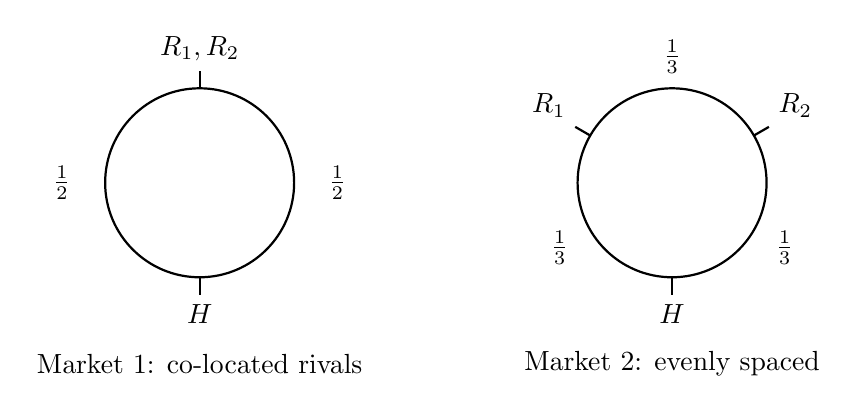
\begin{tikzpicture}[scale=1.0]
  \begin{scope}
    \draw[thick] (0,0) circle (1.2);
    \foreach \a/\lab/\pos in {90/{$R_1,R_2$}/above, 270/{$H$}/below}{
      \draw[thick] (\a:1.2) -- (\a:1.42);
      \node[\pos] at (\a:1.42) {\lab};
    }
    \node at (-1.75,0) {$\frac{1}{2}$};
    \node at (1.75,0) {$\frac{1}{2}$};
    \node at (0,-2.3) {Market 1: co-located rivals};
  \end{scope}
  \begin{scope}[xshift=6cm]
    \draw[thick] (0,0) circle (1.2);
    \foreach \a/\lab/\pos in {150/{$R_1$}/above left, 30/{$R_2$}/above right, 270/{$H$}/below}{
      \draw[thick] (\a:1.2) -- (\a:1.42);
      \node[\pos] at (\a:1.42) {\lab};
    }
    \node at (90:1.6) {$\frac{1}{3}$};
    \node at (210:1.65) {$\frac{1}{3}$};
    \node at (330:1.65) {$\frac{1}{3}$};
    \node at (0,-2.3) {Market 2: evenly spaced};
  \end{scope}
\end{tikzpicture}
\caption{The two hypothetical markets of the theory. Each circle has circumference one, and the fractions give the
arc lengths between neighboring hospitals. In market 1 the rivals $R_1$ and $R_2$ are co-located opposite $H$. In
market 2 the three hospitals are evenly spaced. Redrawn from \citet{Dafny2005}, Figure 1.}
\label{fig:11-dafny}
\end{figure}

Consider market 1 before the rivals merge. Co-located rivals are undifferentiated Bertrand competitors, so they
price at cost, $p_{R}=0$. A consumer at distance $x$ from $H$ is at distance $\frac{1}{2}-x$ from the rivals. She
buys from $H$ if $p_H+tx\le t(\frac{1}{2}-x)$, that is if $x\le\frac{1}{4}-\frac{p_H}{2t}$. Counting both sides of
$H$, its profit is
\begin{equation*}
\pi_H=p_H\cdot2\Big(\frac{1}{4}-\frac{p_H}{2t}\Big).
\end{equation*}
The first-order condition $\frac{1}{2}-\frac{2p_H}{t}=0$ gives $p_H^*=\frac{t}{4}$. Now let the rivals merge into
one firm $R$ with price $p_R$. The indifferent consumer moves to $x=\frac{1}{4}-\frac{p_H-p_R}{2t}$, and
\begin{equation*}
\pi_H=p_H\cdot2\Big(\frac{1}{4}-\frac{p_H}{2t}+\frac{p_R}{2t}\Big).
\end{equation*}
The first-order condition is $\frac{1}{2}-\frac{2p_H}{t}+\frac{p_R}{t}=0$. By symmetry $p_H=p_R$, so
$p_H^*=\frac{t}{2}$. The merger of co-located rivals doubles $H$'s price. Before the merger the rivals priced at
cost. After it they price like a differentiated firm, and $H$ responds to their higher price.

In market 2 the three hospitals are $\frac{1}{3}$ apart. Before the merger the standard symmetric Salop
equilibrium gives $p_H^*=\frac{t}{3}$. Suppose that after the merger one rival facility closes and the other stays
put, so $H$ and $R$ are $\frac{1}{3}$ apart on one side and $\frac{2}{3}$ on the other. $H$'s demand is
$\frac{1}{6}+\frac{p_R-p_H}{2t}$ on the short arc plus $\frac{1}{3}+\frac{p_R-p_H}{2t}$ on the long arc. Profit
$p_H(\frac{1}{2}+\frac{p_R-p_H}{t})$ gives the condition $\frac{1}{2}+\frac{p_R}{t}-\frac{2p_H}{t}=0$, so
$p_H^*=\frac{t}{2}$ at the symmetric equilibrium. The increase is from $\frac{t}{3}$ to $\frac{t}{2}$, or 50\%,
against 100\% in market 1. Mergers of co-located rivals raise prices more because the merger removes a fiercer
pre-merger rivalry.

These formulas hold when $t$ is small relative to $v$, so that every consumer buys and the hospitals compete for
the marginal consumer. Market 1 requires $t<\frac{4v}{3}$ after the merger and market 2 requires
$t<\frac{6v}{5}$. For larger $t$ the marginal consumer's reservation value binds, and demand has a kink. Dafny's
Appendix 1 gives the full solutions:
\begin{align*}
\text{Market 1:}\quad
p_H^{*,pre}&=\begin{cases}\frac{t}{4}, & t<\frac{8v}{3},\\[2pt] 2v-\frac{t}{2}, & \frac{8v}{3}<t<3v,\\[2pt] \frac{v}{2}, & t>3v,\end{cases}
&
p_H^{*,post}&=\begin{cases}\frac{t}{2}, & t<\frac{4v}{3},\\[2pt] v-\frac{t}{4}, & \frac{4v}{3}<t<2v,\\[2pt] \frac{v}{2}, & t>2v,\end{cases}\\[4pt]
\text{Market 2:}\quad
p_H^{*,pre}&=\begin{cases}\frac{t}{3}, & t<2v,\\[2pt] v-\frac{t}{6}, & 2v<t<3v,\\[2pt] \frac{v}{2}, & t>3v,\end{cases}
&
p_H^{*,post}&=\begin{cases}\frac{t}{2}, & t<\frac{6v}{5},\\[2pt] v-\frac{t}{3}, & \frac{6v}{5}<t<\frac{3v}{2}.\end{cases}
\end{align*}
In the middle ranges the hospitals price so that the consumer midway between them gets zero surplus. Take market 1
before the merger. Consumers within $\frac{v}{t}$ of the rivals buy from them at price zero. $H$ can sell to
everyone else only if the consumer at distance $\frac{1}{2}-\frac{v}{t}$ from $H$ gets zero surplus from $H$. That
condition gives $p_H=v-t(\frac{1}{2}-\frac{v}{t})=2v-\frac{t}{2}$.\footnote{For market 2 after the merger, the
appendix gives $\frac{v}{2}$ for all $t>\frac{3v}{2}$. Our derivation differs on part of this range. For
$\frac{3v}{2}<t<3v$ the two remaining hospitals are local monopolists on the long arc but still compete on the
short arc. Their symmetric equilibrium price is $\frac{2v}{5}+\frac{t}{15}$ for $\frac{3v}{2}<t<\frac{18v}{7}$ and
$v-\frac{t}{6}$ for $\frac{18v}{7}<t<3v$, and it is $\frac{v}{2}$ only for $t>3v$. We checked numerically that these
prices are equilibria and that $\frac{v}{2}$ is not. The difference lies outside
the range used for the comparison in the text.} \Cref{fig:11-dafny-prices} plots the solutions with $v=1$.

\begin{figure}[htbp]
\centering
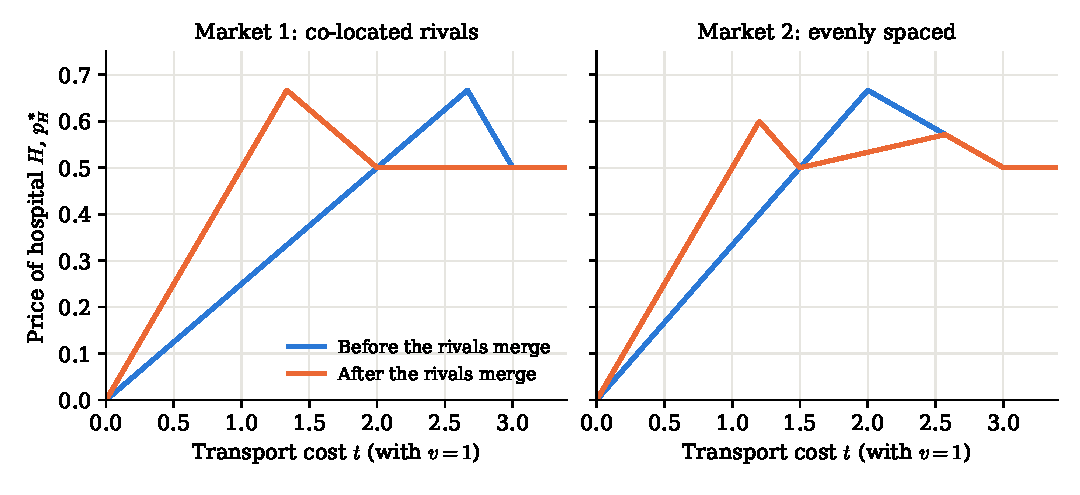
\includegraphics[width=0.95\textwidth]{figures/ch11/dafny_salop_prices.pdf}
\caption{Equilibrium price of hospital $H$ before and after its two rivals merge, as a function of the transport
cost $t$, with $v=1$. Left: co-located rivals. Right: evenly spaced hospitals, one of whose rival facilities closes
after the merger. Solutions from \citet{Dafny2005}, Appendix 1, with the market-2 post-merger curve for
$t>\frac{3}{2}$ derived in the footnote.}
\label{fig:11-dafny-prices}
\end{figure}

Dafny reports that with $v=1$ the average price increase is 66.7\% in market 1 and 40\% in market 2 (footnote 37).
We can reproduce these numbers as percentage gaps between average post-merger and average pre-merger prices. The
averages are taken over the range of $t$ in which the post-merger hospitals still compete, $t<2v$ in market 1 and
$t<\frac{3v}{2}$ in market 2. In
market 1 the average pre-merger price over $(0,2)$ is $0.250$ and the average post-merger price is $0.417$. In market
2 the averages over $(0,\frac{3}{2})$ are $0.250$ and $0.350$. Two predictions follow. Co-located hospitals are more
likely to merge, because they gain more market power and can cut duplicate departments. And a merger of
co-located rivals raises the prices of nearby hospitals by more. The number of co-located rival pairs near a
hospital is therefore a candidate instrument for exposure to rival mergers.

\casehead{Setting} Until 1984 hospitals were paid largely on a cost-plus basis. Medicare's Prospective Payment
System of 1984 paid a fixed amount per admission in each diagnosis-related group, and by 1989 most hospitals lost
money on Medicare patients. Managed care rose from under 30\% of private insurance in 1988 to nearly 95\% by 1999,
replacing fee-for-service payment with negotiated prices. There were 190 hospital mergers between 1989 and 1996,
against 74 between 1983 and 1988. Since 1991 the agencies had tried to block seven hospital mergers and lost every
time, often because courts accepted that non-profit hospitals would not exploit market power (printed pp.~8--9).

\casehead{Data} Merger data come from \citet{DranoveLindrooth2003}, who identify 97 independent hospital mergers
between 1989 and 1996. An independent merger combines two hospitals outside any system into a single entity that
reports one set of accounts and surrenders a license. The sample starts from general, non-federal hospitals in the
1988 American Hospital Association survey, located in metropolitan areas or counties with more than 100,000
residents. Price comes from Medicare cost reports. It is non-Medicare inpatient revenue per case-mix-adjusted
non-Medicare discharge, with charges deflated by each hospital's contractual discounts and Medicare's case-mix
index as a proxy for the non-Medicare one. The tails at the 5th and 95th percentiles are censored. Co-location is
measured from geocoded addresses. Two hospitals are co-located if they are within 0.3 miles as the crow flies and
no more than five blocks apart. Of 213 hospitals within 0.3 miles of another, 191 (3.6\% of 5,373) pass the map
check (printed pp.~12--15).

\Cref{tab:11-dafny-data} summarizes the two samples. In the All Hospitals sample of 4,487 hospitals, 178 (4.0\%)
merged and 163 (3.6\%) were co-located. Eighteen of the 163 merged, a rate of 11\% against 3.7\% for other hospitals.
The Rivals Sample contains the 877 non-merging hospitals with at least two rivals within 7 miles and complete price
data. Of these, 118 had a merging rival (NMW, for non-merging with merging rivals) and 759 did not (NMWO). The two
groups differ. NMW hospitals have nearly twice as many rivals, more Medicaid patients and slightly higher penetration of health maintenance organizations (HMOs).
Their prices grew by $-2.9\%$ between 1985 and 1988, against $4.2\%$ for NMWO hospitals. Treating rival mergers as
exogenous would therefore understate their effect.

\begin{table}[htbp]
\centering
\caption{Hospital mergers: sample means}
\label{tab:11-dafny-data}
\footnotesize
\begin{tabular}{@{}lcccc@{}}
\toprule
& All hospitals & \multicolumn{3}{c}{Rivals Sample} \\
\cmidrule(l){3-5}
& & All & NMW & NMWO \\
\midrule
1988 price (\$ of 2000) & 3,404 & 4,057 & 3,737 & 4,107 \\
1997 price (\$ of 2000) & 3,851 & 4,091 & 3,823 & 4,133 \\
$\ln p_{1988}-\ln p_{1985}$ & 0.064 & 0.032 & $-0.029$ & 0.042 \\
$\ln p_{1997}-\ln p_{1988}$ & 0.132 & 0.010 & 0.020 & 0.009 \\
$\ln p_{2000}-\ln p_{1997}$ & 0.013 & 0.001 & 0.039 & $-0.005$ \\
Merged, 1989--1996 (\%) & 4.0 & & & \\
Co-located (\%) & 3.6 & & & \\
Number of rival mergers, $R_i$ & & 0.156 & 1.161 & 0 \\
Number of co-located rival pairs, $Z_i$ & & 0.332 & 0.712 & 0.273 \\
Number of rivals within 7 miles & 3.16 & 7.37 & 12.03 & 6.64 \\
Medicaid share of discharges (\%) & 11.4 & 11.2 & 15.1 & 10.6 \\
County HMO penetration (\%) & 14.5 & 21.3 & 23.7 & 20.9 \\
Hospitals & 4,487 & 877 & 118 & 759 \\
\bottomrule
\end{tabular}

\smallskip
\begin{minipage}{0.9\linewidth}
\footnotesize Notes: NMW (NMWO) are non-merging hospitals with (without) a rival within 7 miles that merged in
1989--1996. Price change variables are censored at the 5th and 95th percentiles. Characteristics are for 1988,
HMO penetration for 1994. Selected rows. Source: \citet{Dafny2005}, Table 1.
\end{minipage}
\end{table}

\casehead{Estimating equations} For hospital $i$ in the Rivals Sample, let $R_i$ be the number of rival mergers
within 7 miles between 1989 and 1996. Let $Z_i$ be the number of co-located rival pairs within 7 miles in 1988,
excluding any pair to which $i$ belongs. Let $X_i$ be a vector of 1988 hospital and market characteristics. The outcome is
the change in log price between 1988 and 1997, $\Delta\ln p_i$, which spans the year before the first merger to the
year after the last. Because the instrument predicts whether but not when a rival merges, the design uses one
long difference. The equations are
\begin{align}
\text{first stage:}\qquad & R_i=\pi Z_i+X_i^{\top}\omega_F+u_i,\label{eq:11-dafny-fs}\\
\text{reduced form:}\qquad & \Delta\ln p_i=\phi Z_i+X_i^{\top}\omega_R+\varepsilon^{R}_i,\label{eq:11-dafny-rf}\\
\text{structural equation:}\qquad & \Delta\ln p_i=\beta R_i+X_i^{\top}\omega+v_i.\label{eq:11-dafny-iv}
\end{align}
Here $\varepsilon^R_i$ is an error term.\footnote{Here $\varepsilon^R_i$ denotes a regression error, not an
elasticity.} The coefficient $\beta$ is the effect of one rival merger on a hospital's price growth. OLS on
\eqref{eq:11-dafny-iv} is biased if $\Cov(R_i,v_i)\neq0$. The NMW and NMWO comparison above suggests that markets
with mergers had weaker price growth for other reasons, which biases OLS downward.

\casehead{The IV estimator} With one endogenous regressor and one instrument, the model is exactly identified. Let
$\tilde Z_i$ be the residual from regressing $Z_i$ on $X_i$. By the Frisch-Waugh-Lovell theorem, the OLS
coefficients on $Z_i$ in \eqref{eq:11-dafny-fs} and \eqref{eq:11-dafny-rf} are
$\hat\pi=\frac{\sum_i\tilde Z_iR_i}{\sum_i\tilde Z_i^2}$ and
$\hat\phi=\frac{\sum_i\tilde Z_i\Delta\ln p_i}{\sum_i\tilde Z_i^2}$. The IV estimator of $\beta$ is
\begin{equation}\label{eq:11-wald}
\hat\beta_{IV}=\frac{\sum_i\tilde Z_i\,\Delta\ln p_i}{\sum_i\tilde Z_i\,R_i}=\frac{\hat\phi}{\hat\pi},
\end{equation}
the ratio of the reduced-form coefficient to the first-stage coefficient. Substituting \eqref{eq:11-dafny-iv} shows
$\hat\beta_{IV}=\beta+\frac{\sum_i\tilde Z_iv_i}{\sum_i\tilde Z_iR_i}$, which converges to $\beta$ under two
conditions (\cref{app:econometrics}). \emph{Relevance} requires $\pi\neq0$. \emph{Exclusion} requires
$\E[\tilde Z_iv_i]=0$. Co-location of rivals must affect price growth only through the mergers it induces. Suppose the
effect of a rival merger differs across hospitals and co-location never makes a merger less likely. IV then
estimates a weighted average of the effects of the mergers that co-location induces \citep{ImbensAngrist1994}.

Dafny defends exclusion on three grounds. Location is nearly fixed. There has been very little hospital entry since
the Hill-Burton Act of 1946, so co-location in 1988 cannot reflect entry in anticipation of price growth during
1988--1996. Fewer than 1\% of sample hospitals had a rival that exited, and controlling for exits leaves the results
unchanged (footnote 27). The theory is then used to sign the most likely omitted factor, the growth of managed
care. Managed care lowered buyers' willingness to pay, which acts like a fall in $v$. In the solutions above, $v$
matters only in the kinked ranges, where the pre-merger price falls two for one with $v$ in market 1 and one for one
in market 2. Dafny argues that over the relevant range of $t$, prices are at least as sensitive to $v$ where rivals
are co-located. The spread of managed care should then, if anything, slow price growth in those markets and bias
the estimate toward zero (printed p.~22). Finally, the exclusion restriction has testable implications, discussed
next.

\casehead{Results} \Cref{tab:11-dafny} collects the main estimates. Co-location raises a hospital's own probability
of merging by 6.6 percentage points (6.2 with state fixed effects). In the Rivals Sample one more co-located rival
pair raises the number of rival mergers by 0.119 (0.112 with state fixed effects), against a mean of 0.16. The
implied first-stage $F$ statistic is about $(\frac{0.119}{0.018})^2\approx44$, so the instrument is strong. The
reduced form for 1988--1997 is 0.045, against mean price growth of 0.010. The IV estimate is the ratio
\eqref{eq:11-wald}:
\begin{equation*}
\hat\beta_{IV}=\frac{\hat\phi}{\hat\pi}=\frac{0.045}{0.119}\approx0.376,\qquad e^{0.376}-1\approx46\%.
\end{equation*}
The ratio of the rounded coefficients is 0.378. The paper reports 0.376, which equals the ratio of the unrounded
coefficients (footnote 29). With state fixed effects the estimate is 0.301, or about 35\%. A rival merger thus raised
nearby hospitals' prices by about 40\%, enough to move a hospital from the 25th to the 65th percentile of price
growth. OLS gives 0.016 and $-0.003$, both insignificant, and a Hausman test rejects their equality with the IV
estimates.

\begin{table}[htbp]
\centering
\caption{Hospital mergers: first stage, reduced forms and the effect of rival mergers}
\label{tab:11-dafny}
\footnotesize
\begin{tabular}{@{}llccc@{}}
\toprule
Equation & Dependent variable & Without state FE & With state FE & $N$ \\
\midrule
\multicolumn{5}{@{}l}{\textit{A. First stage: coefficient on co-location}} \\
Own merger on own co-location & Merged, 1989--1996 & 0.066 (0.016) & 0.062 (0.016) & 4,487 \\
Rival mergers on $Z_i$, \eqref{eq:11-dafny-fs} & $R_i$ & 0.119 (0.018) & 0.112 (0.019) & 877 \\
\addlinespace
\multicolumn{5}{@{}l}{\textit{B. Reduced form: coefficient on $Z_i$, \eqref{eq:11-dafny-rf}}} \\
Placebo, before the wave & $\ln p_{1988}-\ln p_{1985}$ & $-0.016$ (0.010) & $-0.013$ (0.011) & 877 \\
Treatment period & $\ln p_{1997}-\ln p_{1988}$ & 0.045 (0.014) & 0.034 (0.015) & 877 \\
Placebo, after the wave & $\ln p_{2000}-\ln p_{1997}$ & $-0.008$ (0.013) & $-0.001$ (0.014) & 703 \\
\addlinespace
\multicolumn{5}{@{}l}{\textit{C. Effect of rival mergers on $\ln p_{1997}-\ln p_{1988}$, \eqref{eq:11-dafny-iv}}} \\
IV, instrument $Z_i$ & & 0.376 (0.132) & 0.301 (0.147) & 877 \\
OLS & & 0.016 (0.026) & $-0.003$ (0.027) & 877 \\
\bottomrule
\end{tabular}

\smallskip
\begin{minipage}{0.97\linewidth}
\footnotesize Notes: Standard errors in parentheses. All specifications include the hospital characteristics
(ownership, teaching status, Medicaid share, debt-to-asset ratio, occupancy, bed-size categories) and market
characteristics (metropolitan-area population categories, HMO penetration, log per-capita income). Panel A, first row: All
Hospitals sample, linear probability model. Other rows: Rivals Sample. Source: \citet{Dafny2005}, Tables 2, 3 and
4.
\end{minipage}
\end{table}

\casehead{Tests of the exclusion restriction} The reduced forms in Panel B are falsification tests. Co-located rival
pairs predict price growth only during the merger wave. Before it (1985--1988) the coefficient is small and
negative, and after it (1997--2000) it is close to zero. The mergers thus appear to have caused a one-time increase
in price levels, with no lasting change in trend. The pre-period test matters because NMW hospitals had lower
pre-period growth in the raw data. An overidentification test uses two instruments, the numbers of rival pairs less
than 0.2 miles apart and 0.2 to 0.3 miles apart. The statistic $N R^2$ from regressing the 2SLS residuals on all
exogenous variables is 0.36, with a $p$-value of 0.55 under a $\chi^2(1)$ distribution \citep{Hausman1983}. Such a
test has power only against violations that differ between the two distance bands.

\casehead{Robustness} \Cref{tab:11-dafny-rob} reports the main sensitivity checks. Across co-location definitions
the 7-mile estimates range from 0.326 to 0.511. The market radius matters more. With a 5-mile radius the estimates
more than double, and with 10 miles they are small and insignificant. Effects concentrated on the closest rivals are
what the spatial model predicts, and they suggest that hospital markets are smaller than the 15 to 20 miles often
assumed. Dropping all controls barely changes the estimate (0.352 against 0.380 in the baseline of the appendix
table). By the logic of \citet{AltonjiElderTaber2005}, this stability suggests that unobserved characteristics,
if they relate to the instrument as the observed ones do, do not drive the result. Controlling for the number of
rivals, dropping co-located hospitals, using a negative binomial first stage, or using price levels gives estimates
of the same sign and similar size.

\begin{table}[htbp]
\centering
\caption{Hospital mergers: sensitivity of the IV estimate}
\label{tab:11-dafny-rob}
\footnotesize
\begin{tabular}{@{}lcccc@{}}
\toprule
\multicolumn{5}{@{}l}{\textit{A. Market radius and co-location definition}} \\
& 0.2 miles & 0.3 miles & 0.3 miles and $\le5$ blocks & 0.4 miles \\
\midrule
5 miles ($N=722$) & 0.992 (0.687) & 0.851 (0.340) & 0.962 (0.377) & 1.116 (0.603) \\
7 miles ($N=877$) & 0.511 (0.298) & 0.326 (0.125) & 0.376 (0.132) & 0.431 (0.221) \\
10 miles ($N=1{,}041$) & 0.046 (0.082) & 0.038 (0.050) & 0.051 (0.054) & 0.021 (0.072) \\
\bottomrule
\end{tabular}

\bigskip
\begin{tabular}{@{}lcc@{}}
\toprule
\multicolumn{3}{@{}l}{\textit{B. Specification checks (7 miles, 0.3 miles and $\le5$ blocks)}} \\
Specification & Estimate & $N$ \\
\midrule
(1) Baseline & 0.380 (0.132) & 877 \\
(2) No hospital or market controls & 0.352 (0.132) & 877 \\
(3) Dependent variable not censored & 0.402 (0.143) & 877 \\
(4) Dummies for the number of rivals & 0.408 (0.198) & 877 \\
(5) Co-located hospitals dropped & 0.326 (0.122) & 816 \\
(6) Negative binomial first stage & 0.222 (0.099) & 877 \\
(7) Change in price level (\$ of 2000) & 1,566 (563) & 877 \\
\bottomrule
\end{tabular}

\smallskip
\begin{minipage}{0.9\linewidth}
\footnotesize Notes: 2SLS estimates of $\beta$ in \eqref{eq:11-dafny-iv} without state fixed effects, standard
errors in parentheses. Panel A, column 3, row 2 is the main specification of \cref{tab:11-dafny}. Panel B, row 1
is printed as 0.380 in the appendix table and as 0.376 in the main table. Source: \citet{Dafny2005}, Table 5 and
Appendix Table 1.
\end{minipage}
\end{table}

\casehead{Interpretation} The estimates imply large price increases by the rivals of merging hospitals, about 40\%
per rival merger. Prior longitudinal studies, which compared merging and non-merging hospitals or treated rival
mergers as exogenous, found no effect or a negative one \citep{ConnorFeldman1998}. The OLS estimates here reproduce
that null, and the IV estimates show it to be a selection artifact. The magnitudes are close to those of
structural models of hospital choice, which predict increases of 10\% to 58\% for hypothetical mergers in markets
with few competitors \citep{CappsDranoveSatterthwaite2003,GaynorVogt2003}. Those predictions ignore rivals'
responses and may be too low for that reason (footnote 35). The retrospective thus supports prospective structural
analysis of hospital mergers. Combined with the 14\% cost reductions that \citet{DranoveLindrooth2003} find for the
same type of merger, the results imply large profit gains for merging hospitals.

\casehead{Limitations} The estimate is local. It measures the effect of the rival mergers that co-location induces,
which are mergers of undifferentiated hospitals with unusually large gains in market power. It measures rivals'
responses and says nothing direct about the merging hospitals' own prices, which may rise more or less. The
specification is linear in the number of rival mergers and ignores distance within the 7-mile circle. The price
measure relies on list charges, a contractual discount factor and the Medicare case-mix index. Prices are
negotiated with insurers, so the outcome reflects bargaining between hospitals and managed-care plans, which the
Salop model abstracts from \citep{GalOr1999,CappsDranoveSatterthwaite2003,Ho2009}. \citet{GowrisankaranNevoTown2015}
build this bargaining into a merger simulation for hospitals. They combine the simulation method of
\cref{sec:11-simulation} with the Nash-in-Nash bargaining framework of \citet{CrawfordYurukoglu2012}. They find
that insurers' bargaining power can substantially counteract the market power that hospital mergers create
\citep[p.~238]{AskerNocke2021}. The exclusion restriction can
fail if co-located hospitals sit in old urban cores whose demand evolved differently during the 1990s. The placebo
regressions address this concern only for the years around the wave. Finally, the long difference uses only
cross-sectional variation, so the timing of mergers is not exploited.

\casehead{Contribution} The paper shows how to combine rival analysis with an instrument, so that a retrospective
can address the selection of mergers. It produced the first observational evidence of large price effects of
hospital mergers and showed that relevant hospital markets are small. It also lent support to the structural models
used to evaluate proposed hospital mergers. The idea transfers to other industries in which distance in physical or
product space shifts the propensity to merge.

\subsection{What the retrospective literature finds}\label{sec:11-retro-lit}

The three studies above are part of a growing literature. \citet[Section 3.7 and Appendix A]{AskerNocke2021} survey
the retrospectives published between 2000 and 2020 in the leading general-interest journals and the main industrial
organization journals. For each study they record the date of the transaction, the country and the industry, and
they quote the sentence that best states the authors' conclusion. They chose quotes over a standardized measure of
the price effect, because studies differ too much in units, outcomes and focus (p.~256, n.~201).

Three selection issues limit what the collection can teach \citep[pp.~255--256]{AskerNocke2021}. First, the studied
mergers were cleared by the authorities, so blocked and deterred mergers are absent (\cref{sec:11-retro-select}).
Second, the studies come from industries where data are available, which tilts the sample toward consumer-facing
markets and regulated industries with administrative data. Few retrospectives study intermediate goods. Third, the
studied mergers tend to be large or to offer a chance to study some phenomenon of interest. The collection is not a
random sample of cleared mergers.

Five themes emerge \citep[p.~257]{AskerNocke2021}.
\begin{enumerate}[label=(\roman*)]
\item The price effects vary widely. Some prices rise, at times by a lot, others do not move, and some fall. Asker
and Nocke find this range the most striking feature of the literature.
\item Few studies estimate the change in consumer welfare. Many treat price changes as a sufficient statistic.
\item The outcome variables differ. Most studies measure the prices of the merging firms' products. Some also measure
rivals' prices, and others measure quantities or market shares.
\item Few studies examine longer-run dynamics. \citet{FocarelliPanetta2003} compare short-run and long-run price
effects, and \citet{IgamiUetake2019} study innovation.
\item Few retrospectives study product quality, variety, entry and exit, or investment.
\end{enumerate}
\Cref{tab:11-retro-lit} reproduces a selection of the entries, chosen to cover the range of industries and findings.
Read together, the studies show that consummated mergers can harm consumers, which supports the value of merger
review. The range of outcomes also argues for evaluating each merger in the context of its industry
\citep[p.~257]{AskerNocke2021}.

\begin{table}[htbp]
\centering
\caption{A selection of merger retrospectives}
\label{tab:11-retro-lit}
\footnotesize
\setlength{\tabcolsep}{3pt}
\begin{tabularx}{\textwidth}{@{}>{\raggedright\arraybackslash}p{1.45cm}>{\raggedright\arraybackslash}p{1.16cm}%
>{\raggedright\arraybackslash}p{1.91cm}>{\raggedright\arraybackslash}X>{\raggedright\arraybackslash}p{2.15cm}@{}}
\toprule
Date & Country & Industry & Main finding & Study \\
\midrule
\multicolumn{5}{@{}l}{\textit{Single transactions}} \\
1987 & USA & Airlines & Prices rose 5.0 to 6.0 percent on routes that one carrier served and the other could enter,
more than half the rise on routes where the two had competed &
\citet{KwokaShumilkina2010} \\
1997 & USA & Tampons, pads & Always pads up 8 percent and Tampax up 5 percent relative to private label &
\citet{Weinberg2011} \\
1999 & France & Supermarkets & Rivals' affected stores up about 2 percent (1.8 to 2.4), and the merging firms' prices up
4 to 5 percent & \citet{AllainEtAl2017} \\
1999 & USA & Gasoline & No evidence of higher prices & \citet{SimpsonTaylor2008} \\
2001 & Sweden & Beer & Merging firms' prices roughly constant around the merger, other main brewers' prices up
somewhat, divested beers down relative to both & \citet{FribergRomahn2015} \\
2006 & USA & Appliances & Increases for dishwashers and larger ones for dryers, none for refrigerators or washers.
The merged firm's share and product count fell & \citet{AshenfelterHoskenWeinberg2013} \\
2008 & USA & Airlines & Small fare effects where Delta and Northwest competed: insignificant in nonstop markets, 2.3
percent in connecting markets & \citet{Luo2014} \\
\addlinespace
\multicolumn{5}{@{}l}{\textit{Multiple transactions}} \\
1989--1996 & USA & Hospitals & Prices up roughly 40 percent after nearby rivals merge & \citet{Dafny2009} \\
1990--1998 & Italy & Retail banking & Adverse price changes are temporary, and in the long run efficiency gains dominate
& \citet{FocarelliPanetta2003} \\
1993--2000 & Canada & Mortgages & Significant average rise in interest rates, some borrowers unaffected, and lower price
dispersion & \citet{AllenClarkHoude2014} \\
1996--2006 & USA & Radio & Ad quantity down 11 percent and ad prices up 6 percent. Listener welfare up 0.2 percent,
advertiser welfare down 21 percent & \citet{Jeziorski2014} \\
1996--2015 & Global & Hard disk drives & The rule that blocks mergers when three or fewer firms exist is reasonably
close to maximizing discounted welfare & \citet{IgamiUetake2019} \\
1997--2010 & USA & Dialysis & In more than 1,200 acquisitions, acquired facilities raised doses of highly reimbursed
drugs, replaced skilled nurses with technicians and waitlisted fewer patients. Hospitalizations and mortality rose &
\citet{EliasonEtAl2020} \\
1997--2012 & USA & Hospitals & Of 28 mergers, 9 raised prices and 6 lowered them significantly relative to
controls. Mean change 8.9 percent, median 9.6 percent & \citet{Garmon2017} \\
1998--2000 & USA & Consumer goods & Four of five mergers raised some prices, typically by 3 to 7 percent &
\citet{AshenfelterHosken2010} \\
1998--2006 & USA & Health insurance & Premiums about 7 percentage points higher by 2007 from rising local
concentration, and monopsony power over physicians & \citet{DafnyDugganRamanarayanan2012} \\
2007--2011 & USA & Hospitals & Of 366 mergers, prices up more than 6 percent when the hospitals were within about 5
miles, no effect beyond about 25 miles & \citet{CooperEtAl2019} \\
2007--2008 & USA & Grocery & Five mergers raised prices by more than 2 percent (four in highly concentrated
markets), five lowered them by more than 2 percent, four had little effect & \citet{HoskenOlsonSmith2018} \\
\bottomrule
\end{tabularx}

\vspace{3pt}
\begin{minipage}{\textwidth}
\footnotesize Notes: Paraphrased from the quotations collected by \citet[Appendix A, pp.~262--265]{AskerNocke2021},
whose table lists the date of the transaction, the country, the industry and a quotation from each paper. The
radio entry was also checked against the author's manuscript of \citet{Jeziorski2014}. The appliance, hospital
(1989--1996) and consumer-goods entries are studied in \cref{sec:11-ah,sec:11-maytag,sec:11-dafny}.
\end{minipage}
\end{table}

\section{Does merger simulation work? The Swedish analgesics merger}\label{sec:11-bv}

A merger simulation (\cref{sec:11-simulation}) makes a prediction that can be checked. If a simulated merger is
later consummated, a retrospective of the kind developed in \cref{sec:11-retro} measures its actual effects, and the
two can be compared. Such validation studies are rare, because they need a merger that was simulated or could be
simulated with pre-merger data, and post-merger data on the same market. \citet{BjornerstedtVerboven2016} carry out
one for a merger of painkiller producers in Sweden. They built the simulation for the Swedish Competition Authority
during its review, before the outcome was known. A few years later they compared its predictions with what
happened.\footnote{We use pp.~134, 137 and 147 of the published article, which contain its Figures 1 and 2 and its
Table 6, and its abstract. The institutional facts, the data, the estimating equations, the instruments and the
robustness checks come from the January 2013 working paper \citep{BjornerstedtVerboven2013}. The published version
adds random coefficients models and re-estimates the nested logit, so the working-paper numbers differ from those of
its Table 6.}

\subsection{Question and setting}\label{sec:11-bv-setting}

\casehead{Question} Do the merger simulations used by competition authorities predict the price effects of actual
mergers? And which modeling choices matter for the answer?

\casehead{Setting} The market is over-the-counter analgesics in Sweden. Products differ by active substance
(paracetamol, ibuprofen and acetylsalicylic acid, ASA, sold as aspirin), by administrative form (ordinary tablets
and effervescent, or fizzy, tablets), and by brand, pack size and dose. In 2008 paracetamol held 42.1 percent of
sales value, ibuprofen 29.0 percent and ASA 28.9 percent \citep[Table 1]{BjornerstedtVerboven2013}. Paracetamol and
ibuprofen are sold mainly as tablets, and ASA mainly as fizzy tablets.

GlaxoSmithKline (GSK) notified its acquisition of AstraZeneca Tika (AZT) on December 22, 2008. The Swedish
Competition Authority cleared it on April 3, 2009 \citep[p.~6]{BjornerstedtVerboven2013}. The two firms were the
only sellers of paracetamol \citep[p.~137]{BjornerstedtVerboven2016}. AZT sold Alvedon, with 29.3 percent of 2008
sales value, and Reliv, with 2.2 percent. GSK sold Panodil, with 10.6 percent. McNeil led the other two segments,
with Ipren in ibuprofen (19.1 percent) and Treo and Magnecyl in ASA (25.6 percent together). Nycomed, Meda and Bayer
held the remaining 13.2 percent \citep[Table 2]{BjornerstedtVerboven2013}.

Until 2009 all sales went through the state pharmacy monopoly, Apoteket AB. It added a fixed percentage markup to
the producers' wholesale prices and charged the same price in every pharmacy, so producers set retail prices
indirectly \citep[pp.~6 and~9]{BjornerstedtVerboven2013}. The authority cleared the merger on two grounds. It
judged that consumers choose brands more than substances. It also expected the deregulation of pharmacies, decided
for 2009, to bring entry and stronger buyers. Its decision cited the authors' simulation as showing no significant
price increase. The authors note that their simulations predicted an insignificant increase only in a scenario with
large efficiencies (pp.~6--8). Entry after the deregulation was surprisingly slow
\citep[p.~134]{BjornerstedtVerboven2016}. Ibuprofen and ASA are therefore the substitutes that discipline the
paracetamol price.

\casehead{Data} During its review the authority obtained monthly sales data for 1995 to 2008 from Apoteket. A
product is a brand, form, pack size and dose, such as Alvedon tablets in packs of 30 pieces of 500 mg. An
observation of product $j$ in month $t$ records the price $p_{jt}$, the volume $q_{jt}$ and the revenue
$r_{jt}=p_{jt}q_{jt}$. Prices include value-added tax and are the prices every consumer paid. The data are merged
with monthly marketing expenditures by brand and with monthly counts of sick men and sick women from Statistics
Sweden. The full sample has 11,185 product-months. The estimation sample keeps the three main substances and the
two main forms. It has 7,240 product-months, about 43 products per month, and covers about 90 percent of sales value
\citep[Section 2.3]{BjornerstedtVerboven2013}. Painkillers have no natural unit of consumption. The authors measure
volume in tablets, in defined daily doses and in normal single doses, and they report results for tablets.
\Cref{tab:11-bv-sum} reproduces the main summary statistics. For the retrospective the authors later obtained the
same data for 2008 to May 2011. The 2008 figures matched those of the original data (p.~10).

\begin{table}[htbp]
\centering
\caption{Swedish analgesics: summary statistics of the estimation sample, 1995--2008}
\label{tab:11-bv-sum}
\footnotesize
\begin{tabular}{@{}lcccc@{}}
\toprule
Variable & Mean & Std.\ dev. & Min. & Max. \\
\midrule
Revenue $r_{jt}$ (million SEK) & 1.24 & 2.56 & 0.00 & 22.95 \\
Price per tablet $p_{jt}$ (SEK) & 1.06 & 0.46 & 0.27 & 2.55 \\
Tablets sold $q_{jt}$ (million) & 1.11 & 2.19 & 0.00 & 16.61 \\
Marketing expenditures & 564.1 & 1{,}445.7 & 0 & 13{,}536 \\
Sick women & 822.9 & 197.0 & 391 & 1{,}204 \\
Sick men & 524.5 & 108.0 & 254 & 763 \\
Nominal GDP (billion SEK) & 621.6 & 107.4 & 443.2 & 859.7 \\
\bottomrule
\end{tabular}

\smallskip
\begin{minipage}{0.8\linewidth}
\footnotesize Notes: 7,240 product-months. Selected rows. The paper does not state the units of marketing
expenditures and of the sickness counts. In December 2008 one euro was 10.8 SEK and one US dollar 8.0 SEK. Source:
\citet{BjornerstedtVerboven2013}, Table 3.
\end{minipage}
\end{table}

\subsection{The retrospective evidence}\label{sec:11-bv-retro}

\Cref{fig:11-bvprice,fig:11-bvshare} show what happened. Paracetamol prices drifted up from about 1.39 kronor in
April 2007 to about 1.50 at the end of 2008. Within two months of the merger they jumped to about 1.99 and stayed
near that level. Ibuprofen prices, at about 1.67, did not move at the merger. ASA prices rose modestly, from about
1.41 to about 1.55 kronor. These readings are taken from the figure.
In logs the plotted paracetamol jump is about $\ln\frac{1.99}{1.50}\approx0.28$, and the ASA increase is about
$\ln\frac{1.55}{1.41}\approx0.10$. The paracetamol share of the analgesics market fell from a peak of about
49\% just before the merger to about 41\%, then recovered to 43\% to 45\%. The ibuprofen share jumped from about
27\% to about 32\%, and the ASA share stayed near 24\% to 26\%. Consumers substituted mainly toward ibuprofen.

\begin{figure}[htbp]
\centering
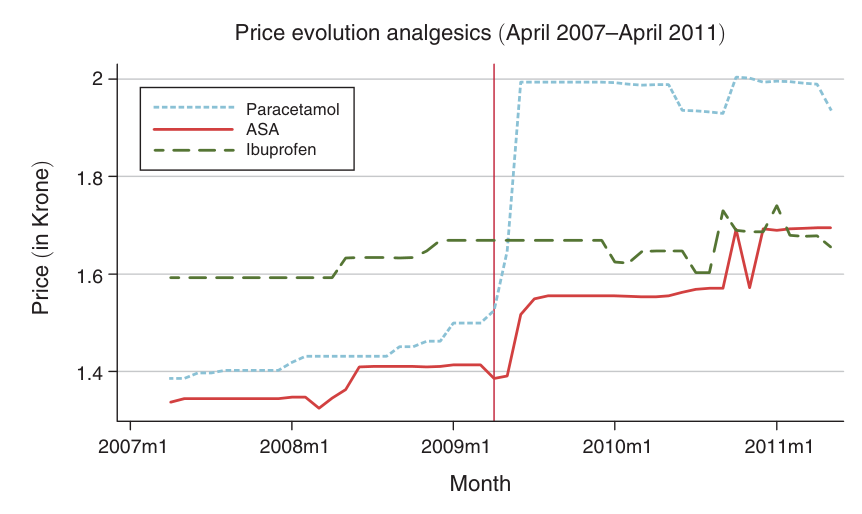
\includegraphics[width=0.72\textwidth]{figures/ch11/bv_fig1_price.png}
\caption{Average prices of paracetamol, ASA and ibuprofen analgesics in Sweden, April 2007 to April 2011, in kronor.
The vertical line marks the merger (April 2009). Source: \citet{BjornerstedtVerboven2016}, Figure 1.}
\label{fig:11-bvprice}
\end{figure}

\begin{figure}[htbp]
\centering
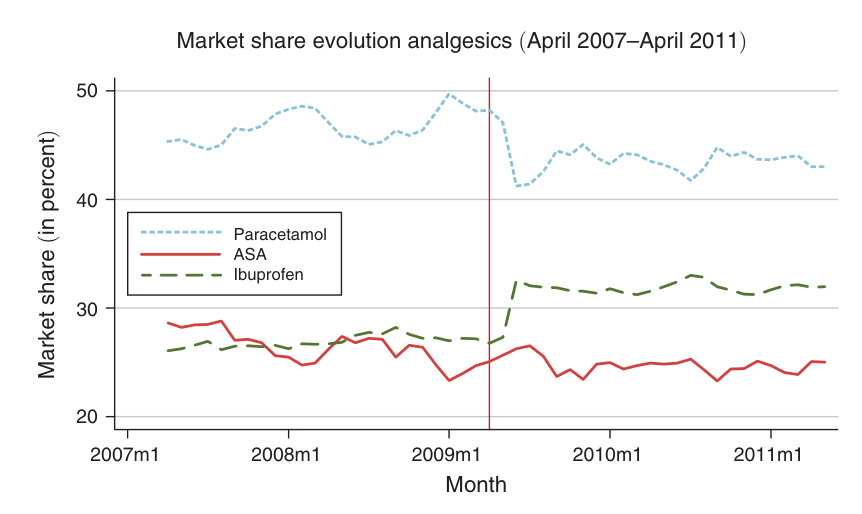
\includegraphics[width=0.72\textwidth]{figures/ch11/bv_fig2_share.png}
\caption{Market shares of paracetamol, ASA and ibuprofen analgesics in Sweden, April 2007 to April 2011, in percent.
The vertical line marks the merger (April 2009). Source: \citet{BjornerstedtVerboven2016}, Figure 2.}
\label{fig:11-bvshare}
\end{figure}

The stability of ibuprofen prices suggests that the paracetamol increase was not caused by a general cost or demand
shock \citep[p.~134]{BjornerstedtVerboven2016}. A regression in the spirit of \citet{AshenfelterHosken2010} makes
the comparison precise:
\begin{equation}\label{eq:11-bv-retro}
\ln p_{gt}=\alpha_g+\beta_g\,\mathit{PostMerger}_t+e_{gt}.
\end{equation}
Here $p_{gt}$ is the average price of product group $g$ in month $t$. The indicator $\mathit{PostMerger}_t$ equals
one after the merger. The published version defines groups by substance and by substance and firm (p.~134). Each group has its
own post-merger change $\beta_g$, which is more general than a common change for all control groups. The difference
between the merging firms' $\beta_g$ and a rival group's $\beta_g$ is a DiD estimate of the merger effect. By
\cref{prop:11-didbias}, a rival control yields a lower bound when rivals raise prices in response.

The published version compares one year before and one year after the merger. The short window keeps out later
effects of the deregulation \citep[p.~134 and eq.~(1)]{BjornerstedtVerboven2016}. The article reports that the
merging firms raised prices by 40 percent and that some outsiders raised prices by more than 10 percent
\citep[abstract]{BjornerstedtVerboven2016}. Its Table~4 gives price changes of 39.7 percent for paracetamol, 0.1
percent for ibuprofen and 13.3 percent for ASA (p.~135). \Cref{tab:11-bv-expost} reports the working paper's
estimates, in log points. They compare two years on each side of the
merger, April 2007 to April 2009 against May 2009 to May 2011, and define groups by substance and by firm
\citep[Table 7]{BjornerstedtVerboven2013}.

The paracetamol price rose by 0.351 log points, or 42 percent. Ibuprofen prices did not move (0.001), and ASA prices
rose by 0.100 log points, or 11 percent. With ibuprofen as the control the DiD estimate is 0.350. With ASA as the
control it is 0.251, or 29 percent. Pooling the two rival substances into one control gives 0.30, or 35 percent
\citep[fn.~17]{BjornerstedtVerboven2013}. The ASA increase is consistent with a rival response, so the ASA-based
estimate understates the effect on paracetamol prices. Both merging firms raised prices by similar amounts, 0.356 log
points for AZT and 0.379 for GSK. Among the outsiders, Bayer raised prices by 0.105 and McNeil by 0.084 log points.
The regressions compare average log prices of product groups over the two windows, so they need not match the jump
in the plotted average price.

The same design applied to volume shares shows where demand went. The paracetamol share fell by 3.3 percentage
points, with a 95 percent confidence interval of 2.7 to 3.9 points. The ibuprofen share rose by 5.0 points, and the
ASA share fell by 1.6 points. AZT lost 5.6 points, while GSK's loss of 0.3 points is insignificant. McNeil lost 2.7
points, and the other outsiders gained a little \citep[pp.~31--32]{BjornerstedtVerboven2013}.

\subsection{The prospective models}\label{sec:11-bv-model}

The simulation has the structure of \cref{sec:11-simulation}: estimate demand on pre-merger data, recover marginal
costs from the pre-merger first-order conditions, change the ownership matrix, and solve for the new equilibrium.
Two demand families are used, each in two versions.

\casehead{Nested logit} Consumer $i$ chooses among products $j\in\mathcal{J}$ and an outside good $j=0$. Products are
grouped into nests $g$, and each nest into subnests $h$. In the authors' maintained specification the nests are the
two administrative forms, and the subnests are the substances within each form
\citep[p.~20]{BjornerstedtVerboven2013}. We first present the one-level version, with nests $g$ only. Its utility is
\begin{equation*}
u_{ij}=\delta_j+\zeta_{ig}+(1-\sigma)\epsilon_{ij},
\end{equation*}
where $\delta_j$ is mean utility, $\epsilon_{ij}$ is type-I extreme value, and $\zeta_{ig}$ has the distribution
that makes $\zeta_{ig}+(1-\sigma)\epsilon_{ij}$ extreme value \citep{Cardell1997}. The nesting parameter
$\sigma\in[0,1)$ measures the correlation of tastes within a nest (\cref{ch:logit}). As in \cref{sec:11-diversion},
let $H_g=\sum_{k\in g}e^{\frac{\delta_k}{1-\sigma}}$. Market shares are
\begin{equation}\label{eq:11-nl-shares}
s_j=s_{j|g}\,s_g,\qquad s_{j|g}=\frac{e^{\frac{\delta_j}{1-\sigma}}}{H_g},\qquad s_g=\frac{H_g^{1-\sigma}}{1+\sum_{g'}H_{g'}^{1-\sigma}},
\end{equation}
and the outside share is $s_0=\frac{1}{1+\sum_{g'}H_{g'}^{1-\sigma}}$.

\begin{lemma}[Nested logit share derivatives]\label{lem:11-nl-deriv}
For products $j\neq k$,
\begin{align*}
\frac{\partial s_j}{\partial\delta_j}&=s_j\Big[\frac{1}{1-\sigma}-\frac{\sigma}{1-\sigma}s_{j|g}-s_j\Big],\\
\frac{\partial s_j}{\partial\delta_k}&=-s_j\Big[\frac{\sigma}{1-\sigma}s_{k|g}+s_k\Big]\quad\text{if $k$ is in $j$'s nest,}\\
\frac{\partial s_j}{\partial\delta_k}&=-s_js_k\quad\text{if $k$ is in another nest.}
\end{align*}
\end{lemma}

\begin{proof}
Taking logs of \eqref{eq:11-nl-shares} gives
$\ln s_j=\frac{\delta_j}{1-\sigma}-\sigma\ln H_g-\ln\big(1+\sum_{g'}H_{g'}^{1-\sigma}\big)$. \Cref{sec:11-diversion}
computed the derivatives of the last two terms on the way to \eqref{eq:11-nl-diversion}. The derivative of $\ln H_g$
with respect to $\delta_k$ is $\frac{s_{k|g}}{1-\sigma}$ for $k\in g$ and zero otherwise. The derivative of the log
of the denominator is $s_k$ for every inside product $k$. Hence $\frac{\partial\ln s_j}{\partial\delta_k}$ equals
$\frac{1}{1-\sigma}-\frac{\sigma}{1-\sigma}s_{j|g}-s_j$ for $k=j$, $-\frac{\sigma}{1-\sigma}s_{k|g}-s_k$ for $k\neq j$
in the same nest, and $-s_k$ for $k$ in another nest. Multiplying each by $s_j$ gives the lemma.
\end{proof}

Inverting \eqref{eq:11-nl-shares} gives the linear estimating equation
$\ln s_j-\ln s_0=\delta_j+\sigma\ln s_{j|g}$ (\cref{ch:logit}). The two-level version adds the subnests $h$ within
each nest $g$, with parameters $0\le\sigma_2\le\sigma_1<1$. Here $\sigma_1$ measures the correlation of tastes
within a subnest and $\sigma_2$ within a nest. With unit demand its estimating equation is
\begin{equation}\label{eq:11-nl2}
\ln s_j-\ln s_0=x_j\beta-\alpha\,p_j+\sigma_1\ln s_{j|hg}+\sigma_2\ln s_{h|g}+\xi_j,
\end{equation}
where $s_{j|hg}$ is $j$'s share of its subnest and $s_{h|g}$ the subnest's share of the nest
\citep[eq.~(9)]{Verboven1996,BjornerstedtVerboven2013}.\footnote{We verified \eqref{eq:11-nl2} and the derivatives
below numerically against the two-level share formulas.} The authors also estimated the reverse order, with
substances as nests and forms as subnests. It gave $\sigma_1<\sigma_2$, which is inconsistent with random utility
maximization, so they kept forms as the nests (p.~20). Let $\vartheta_1=\frac{1}{1-\sigma_1}-\frac{1}{1-\sigma_2}\ge0$,
$\vartheta_2=\frac{\sigma_2}{1-\sigma_2}$ and $s_{j|g}=s_{j|hg}s_{h|g}$. The share derivatives are
\begin{align*}
\frac{\partial s_j}{\partial\delta_j}&=s_j\Big[\frac{1}{1-\sigma_1}-\vartheta_1\,s_{j|hg}-\vartheta_2\,s_{j|g}-s_j\Big],\\
\frac{\partial s_j}{\partial\delta_k}&=-s_j\big[\vartheta_1\,s_{k|hg}+\vartheta_2\,s_{k|g}+s_k\big]\quad\text{(same subnest)},\\
\frac{\partial s_j}{\partial\delta_k}&=-s_j\big[\vartheta_2\,s_{k|g}+s_k\big]\quad\text{(same nest, other subnest)},\\
\frac{\partial s_j}{\partial\delta_k}&=-s_js_k\quad\text{(other nest)}.
\end{align*}
Cross-elasticities are largest within a subnest, smaller between subnests of the same nest, and smallest across
nests. Under the maintained order, the closest substitutes share both form and substance, and the most distant
differ in form. The estimates in \cref{tab:11-bv-demand} below show this ordering.

\casehead{Unit demand and constant expenditures} The two versions differ in how price enters utility and what a
market share measures \citep[Section 3.1]{BjornerstedtVerboven2013}. Consumer $i$, with income $y_i$, gets utility
$u_{ij}=x_j\beta+\xi_j+\alpha f(y_i,p_j)+\epsilon_{ij}$ from product $j$. Conditional on choosing $j$, she buys
$d_{ij}$ units, given by Roy's identity:
\begin{equation*}
d_{ij}=-\dfrac{\frac{\partial f(y_i,p_j)}{\partial p_j}}{\frac{\partial f(y_i,p_j)}{\partial y_i}} .
\end{equation*}
Unit demand sets $f(y_i,p_j)=y_i-p_j$. Both derivatives have absolute value one, so $d_{ij}=1$. Constant
expenditures sets $f(y_i,p_j)=\frac{1}{\gamma}\ln y_i-\ln p_j$ for a constant $\gamma\in(0,1)$. Then
\begin{equation*}
d_{ij}=-\dfrac{-\frac{1}{p_j}}{\frac{1}{\gamma y_i}}=\frac{\gamma y_i}{p_j},
\end{equation*}
so the consumer spends the fraction $\gamma$ of her income on the chosen product. In both versions the income term
is common to all products of consumer $i$, so it drops out of the choice probabilities. These remain the nested logit
formulas, now evaluated at the mean utilities given below. Summing $d_{ij}$ times the choice probability over
consumers gives aggregate demand. With unit demand $q_j=s_jM$, where $M$ is the number of consumers. With constant
expenditures $q_j=\frac{s_jB}{p_j}$, where $B=\gamma\sum_iy_i$ is the potential budget for the category.

In the \emph{unit demand} version each consumer buys at most one unit. Mean utility is linear in price,
$\delta_j=x_j\beta-\alpha p_j+\xi_j$, and shares are volume shares, $s_j=\frac{q_j}{M}$ for a potential number of
units $M$. Since $\frac{\partial\delta_k}{\partial p_k}=-\alpha$, the elasticities in the one-level model are
\begin{align}
\varepsilon_{jj}&=-\alpha\,p_j\Big[\frac{1}{1-\sigma}-\frac{\sigma}{1-\sigma}s_{j|g}-s_j\Big],\label{eq:11-unit-own}\\
\varepsilon_{jk}&=\alpha\,p_k\Big[\frac{\sigma}{1-\sigma}s_{k|g}+s_k\Big]\ \text{(same nest)},\qquad
\varepsilon_{jk}=\alpha\,p_ks_k\ \text{(other nest)},\nonumber
\end{align}
where $\varepsilon_{jj}<0$ is the own-price elasticity in signed form. Elasticities are proportional to price.
Expensive products have more elastic demand, and the own elasticity of a product rises as its price rises.

In the \emph{constant expenditures} version each consumer spends a fixed budget on the category. Mean utility is
linear in log price, $\delta_j=x_j\beta-\alpha\ln p_j+\xi_j$, and shares are value shares,
$w_j=\frac{p_jq_j}{B}$ for a potential budget $B$. The formulas \eqref{eq:11-nl-shares} now give $w_j$. Quantity is
$q_j=\frac{Bw_j}{p_j}$, so $\ln q_j=\ln B+\ln w_j-\ln p_j$, and $\frac{\partial\delta_k}{\partial\ln
p_k}=-\alpha$. The quantity elasticities are
\begin{align}
\varepsilon_{jj}&=-\alpha\Big[\frac{1}{1-\sigma}-\frac{\sigma}{1-\sigma}w_{j|g}-w_j\Big]-1,\label{eq:11-ce-own}\\
\varepsilon_{jk}&=\alpha\Big[\frac{\sigma}{1-\sigma}w_{k|g}+w_k\Big]\ \text{(same nest)},\qquad
\varepsilon_{jk}=\alpha\,w_k\ \text{(other nest)}.\nonumber
\end{align}
These depend on prices only through value shares, so they are roughly constant along the demand curve. The extra
$-1$ in the own elasticity reflects the fixed budget. A higher price lowers the quantity bought even at an unchanged
value share, and that lost quantity is diverted to no other product.

Substituting value shares into the inverted two-level system gives the constant-expenditure estimating equation
\begin{equation}\label{eq:11-ce-est}
\ln w_j-\ln w_0=x_j\beta-\alpha\ln p_j+\sigma_1\ln w_{j|hg}+\sigma_2\ln w_{h|g}+\xi_j,
\end{equation}
where $w_0=1-\sum_kw_k$ is the outside value share. Here $w_{j|hg}$ and $w_{h|g}$ are the value shares within the
subnest and the nest \citep[eq.~(10)]{BjornerstedtVerboven2013}. The equation differs from \eqref{eq:11-nl2} in three ways.
Price enters in logs, shares are measured in value, and the potential market is a budget $B$ rather than a number of
consumers. The authors note that this version had not been used in empirical work, although it is as easy to
estimate as the unit-demand version (pp.~2--3).

The difference matters for mergers through pass-through (\cref{sec:11-passthrough}). Under unit demand, demand becomes
more elastic as price rises, which restrains post-merger price increases. Under constant expenditures, the merged
firm faces roughly constant elasticities and can push prices further. The contrast is the one between linear or
logit demand and the constant-expenditure logit in \cref{fig:11-curvature}.

\casehead{Random coefficients} The nested logit restricts substitution to the hierarchy of nests and subnests. It
also rules out correlated preferences along continuously measured characteristics
\citep[p.~137]{BjornerstedtVerboven2016}. The published version therefore adds the random coefficients logit of
\citet{BerryLevinsohnPakes1995} (\cref{ch:blp}), again in unit-demand and constant-expenditure versions. Tastes for
product characteristics vary across consumers, which yields more flexible substitution patterns. The model has four
random coefficients, on the dummies for fizzy tablets, paracetamol and the branded products (Alvedon, Ipren and
Treo), and on the constant \citep[p.~143]{BjornerstedtVerboven2016}. The price coefficient is common to all
consumers (Table~5). The model needs no prior hierarchy of nests, and the branded-product coefficient allows the
substitution among brands that the competition authority considered relevant.

\casehead{Estimation and identification} Both nested logit equations, \eqref{eq:11-nl2} and \eqref{eq:11-ce-est},
are linear in parameters. The authors estimate them by linear instrumental variables on the panel of product-months
\citep[Section 4.1]{BjornerstedtVerboven2013}. The regressors are price or log price, the two within-group shares,
marketing expenditures and the numbers of sick women and sick men. The equations also include a time trend,
month-of-year dummies and a fixed effect for each of the 56 products. The product effects absorb pack size, dose and other fixed characteristics. The
potential market is twice the average amount bought over the period, in units for unit demand and in value for
constant expenditures.

Price and the two within-group shares are endogenous, because they depend on $\xi_j$. The base instruments are
counts of other products, overall and within the same firm, nest and subnest. The exclusion restriction is the usual
one of \citet{BerryLevinsohnPakes1995}: the set of products on offer is uncorrelated with the demand shocks. With
product effects in the equation, the counts vary only through the entry and exit of products over time. More rivals
in a subnest lower a product's within-subnest share and its markup at fixed own quality, and these shifts identify
$\alpha$, $\sigma_1$ and $\sigma_2$. Marketing is treated as exogenous, on the argument that the product effects
absorb its main correlation with $\xi_j$ (pp.~20--21). The published version estimates the random coefficients
models as in \cref{ch:blp}. The contraction mapping recovers mean utilities from shares, and the parameters are
estimated by GMM as in BLP \citep[p.~158]{BjornerstedtVerboven2016}. A first stage uses the instruments of
\citet{BerryLevinsohnPakes1995}, sums of the characteristics with random coefficients over the firm's other products
and over rivals' products. A second stage uses optimal instruments (\cref{sec:A-optimal-iv}). The share integral is
approximated by a nested quadrature rule (pp.~143--144 and n.~7).

\casehead{Supply and simulation} Firms set prices in a multi-product Bertrand-Nash equilibrium. With $\Omega$ the
ownership matrix and $\Delta$ the matrix of quantity derivatives with elements $\frac{\partial q_j}{\partial p_k}$,
the first-order conditions are $q+(\Omega\odot\Delta)^{\top}(p-mc)=0$. Marginal costs are recovered from these
conditions at pre-merger prices. For a single-product firm under constant expenditures, profit is
$(p_j-c_j)\frac{Bw_j}{p_j}=\big(1-\frac{c_j}{p_j}\big)Bw_j$. Let $\eta_j=\frac{\partial\ln w_j}{\partial\ln
p_j}<0$. Setting the derivative of profit to zero gives
\begin{equation*}
\frac{c_j}{p_j^2}\,w_j+\Big(1-\frac{c_j}{p_j}\Big)\frac{\partial w_j}{\partial p_j}=0
\quad\Longrightarrow\quad
\frac{c_j}{p_j}+\Big(1-\frac{c_j}{p_j}\Big)\eta_j=0
\quad\Longrightarrow\quad
L_j=\frac{p_j-c_j}{p_j}=\frac{1}{1-\eta_j}=\frac{1}{|\varepsilon_{jj}|},
\end{equation*}
the inverse elasticity rule. The merger is simulated by joining AZT and GSK in $\Omega$, with no efficiencies, and
solving the post-merger conditions for prices. The authors solve them by fixed-point iteration, dampened when it
fails to converge, and Newton's method gives the same results \citep[p.~18]{BjornerstedtVerboven2013}.

The working paper also allows \emph{partial coordination}, in which each firm puts a weight $\phi\in(0,1)$ on its
rivals' profits before and after the merger. The zeros of $\Omega$ then become $\phi$. This $\phi$ is unrelated to
the coefficient $\phi$ of \eqref{eq:11-dafny-rf}. The authors set $\phi=0.75$, because it makes the implied
pre-merger marginal costs consistent with cost information available to the authority (pp.~18 and~23).

\subsection{Predictions and outcomes}\label{sec:11-bv-results}

\casehead{Demand estimates} \Cref{tab:11-bv-demand} reproduces the working paper's nested logit estimates. Both
versions satisfy $1\ge\sigma_1\ge\sigma_2\ge0$, with strict inequalities. Products of the same form and substance are
the closest substitutes, products of the same form and another substance come next, and products of another form are
the most distant \citep[p.~21]{BjornerstedtVerboven2013}. Marketing raises demand in both versions, and demand peaks
in December and March. The unit-demand version gives a negative coefficient on sick women, which the authors suspect
picks up other effects. The implied elasticities differ sharply. The average own elasticity is $-2.68$ under
constant expenditures and $-12.4$ under unit demand. The unit-demand range, from $-24.1$ to $-3.9$, is roughly
proportional to the range of prices. The constant-expenditure range is narrow, from $-2.84$ to $-1.91$.

\begin{table}[htbp]
\centering
\caption{Swedish analgesics: nested logit demand estimates in the working paper}
\label{tab:11-bv-demand}
\footnotesize
\begin{tabular}{@{}lcccc@{}}
\toprule
& \multicolumn{2}{c}{Constant expenditures} & \multicolumn{2}{c}{Unit demand} \\
\cmidrule(lr){2-3}\cmidrule(l){4-5}
& Estimate & Std.\ error & Estimate & Std.\ error \\
\midrule
Price coefficient $\alpha$ & 0.304 & 0.101 & 2.042 & 0.157 \\
Subnest parameter $\sigma_1$ (substance) & 0.835 & 0.021 & 0.928 & 0.013 \\
Nest parameter $\sigma_2$ (form) & 0.667 & 0.025 & 0.792 & 0.012 \\
Marketing expenditures & 15.50 & 2.90 & 8.85 & 1.82 \\
Sick women & 0.357 & 0.129 & $-0.699$ & 0.079 \\
Sick men & 1.145 & 0.244 & 0.809 & 0.157 \\
Time trend & 0.0013 & 0.0005 & 0.0007 & 0.0002 \\
$R^2$ & \multicolumn{2}{c}{0.983} & \multicolumn{2}{c}{0.972} \\
\addlinespace
\multicolumn{5}{@{}l}{\textit{Implied elasticities in December 2008: average and standard error}} \\
Own price & $-2.68$ & 0.63 & $-12.4$ & 2.6 \\
Cross, same subnest & 0.164 & 0.068 & 1.45 & 0.38 \\
Cross, other subnest of the same nest & 0.039 & 0.012 & 0.245 & 0.022 \\
Cross, other nest & 0.006 & 0.002 & 0.016 & 0.001 \\
\addlinespace
\multicolumn{5}{@{}l}{\textit{Implied elasticities in December 2008: minimum and maximum}} \\
Own price & $-2.84$ & $-1.91$ & $-24.1$ & $-3.9$ \\
Cross, same subnest & 0.00 & 0.93 & 0.00 & 8.3 \\
Cross, other subnest of the same nest & 0.00 & 0.29 & 0.00 & 1.76 \\
Cross, other nest & 0.00 & 0.06 & 0.00 & 0.16 \\
\bottomrule
\end{tabular}

\smallskip
\begin{minipage}{0.92\linewidth}
\footnotesize Notes: Linear IV estimates of \eqref{eq:11-ce-est} and \eqref{eq:11-nl2} on 7,240 product-months,
1995--2008. Nests are forms and subnests are substances within a form. The paper reports the price coefficient as
$-\alpha$. Price enters in logs under constant expenditures and in SEK per tablet under unit demand. Both regressions
include 56 product fixed effects and month dummies. Robust standard errors. Standard errors of the elasticities use
the delta method for an average product. Source: \citet{BjornerstedtVerboven2013}, Table 4.
\end{minipage}
\end{table}

\casehead{Predictions during the review} The authority received predictions for four scenarios in each version
\citep[Table 5]{BjornerstedtVerboven2013}. Under constant expenditures and Bertrand conduct, the paracetamol price was
predicted to rise by 34.0 percent, or by 4.7 percent with a 25 percent cut in marginal cost. Under partial
coordination the predictions were 28.4 and $-0.1$ percent. Under Bertrand conduct, unit demand predicted 12.9 percent
without the cost cut and 1.6 percent with it. Under partial coordination it predicted 16.1 and 9.0 percent. The implied pre-merger markups were 0.49 and 0.76 under
constant expenditures, and 0.16 and 0.54 under unit demand. The authors preferred constant expenditures for two
reasons. Its elasticities neither rise mechanically with price nor depend on the unit of consumption. Its markups were
also broadly in line with the variable costs reported by the parties, while the unit-demand markups were well below
them (pp.~24--25).

\casehead{The published estimates} \Cref{tab:11-bv} reproduces Table 6 of the published version, which re-estimates
the nested logit and adds the random coefficients models. The four specifications imply very different demand. The
average own-price elasticity is $-2.43$ in the constant-expenditure nested logit and $-8.84$ in the unit-demand
nested logit. The random coefficients logit gives $-2.05$ and $-3.61$. Unit demand also produces a much wider range
of own elasticities across products, from $-5.16$ to $-15.45$ in the nested logit, because elasticities are
proportional to prices. Cross-elasticities are larger within a substance than across substances in every
specification.

\begin{table}[htbp]
\centering
\caption{Swedish analgesics: price elasticities, markups and predicted price effects}
\label{tab:11-bv}
\footnotesize
\begin{tabular}{@{}lcccc@{}}
\toprule
& \multicolumn{2}{c}{Nested logit} & \multicolumn{2}{c}{Random coefficients logit} \\
\cmidrule(lr){2-3}\cmidrule(l){4-5}
& Constant expenditures & Unit demand & Constant expenditures & Unit demand \\
\midrule
\multicolumn{5}{@{}l}{\textit{Brand-level price elasticities}} \\
Own & $-2.43$ & $-8.84$ & $-2.05$ & $-3.61$ \\
Own (range) & ($-3.05$, $-2.00$) & ($-15.45$, $-5.16$) & ($-2.61$, $-1.51$) & ($-6.52$, $-1.99$) \\
Cross, same substance & 0.30 & 2.12 & 0.12 & 0.36 \\
Cross, different substance & 0.05 & 0.28 & 0.05 & 0.19 \\
\addlinespace
\multicolumn{5}{@{}l}{\textit{Markups (percent)}} \\
Paracetamol & 48.5 & 17.3 & 59.0 & 44.7 \\
Ibuprofen & 45.0 & 11.8 & 55.7 & 32.3 \\
ASA & 59.1 & 22.9 & 66.5 & 44.5 \\
\addlinespace
\multicolumn{5}{@{}l}{\textit{Basic predicted price effects (percent)}} \\
Paracetamol & 41.1 & 15.9 & 21.29 & 9.34 \\
Ibuprofen & 1.2 & 0.5 & 0.75 & 0.76 \\
ASA & 1.5 & 0.6 & 0.81 & 0.45 \\
\bottomrule
\end{tabular}

\smallskip
\begin{minipage}{0.95\linewidth}
\footnotesize Notes: All numbers are averages across products for December 2008, except the ranges in
parentheses. Markups are Lerner indices $\frac{p-c}{p}$ implied by the pre-merger Bertrand-Nash conditions. The
predicted price effects merge the two paracetamol sellers, with no efficiencies. Source:
\citet{BjornerstedtVerboven2016}, Table 6.
\end{minipage}
\end{table}

The markups follow from the elasticities. The inverse of the average own elasticity is 41\% in the
constant-expenditure nested logit, 11\% in the unit-demand nested logit, 49\% and 28\% in the two random
coefficients models. The reported markups are higher, for two reasons. Multi-product firms internalize
cannibalization among their own products, which raises markups above the single-product rule. And the average of
$\frac{1}{|\varepsilon_{jj}|}$ across products exceeds the inverse of the average elasticity, because the function
$\frac{1}{x}$ is convex. The second effect is large under unit demand, where the inverse elasticities range from
6.5\% to 19.4\% in the nested logit.

\casehead{Comparison with the outcome} The merging firms raised prices by about 40 percent (\cref{sec:11-bv-retro}).
The prediction made during
the review, 34 percent under constant expenditures and Bertrand conduct, came close. The re-estimated
constant-expenditure nested logit of \cref{tab:11-bv} predicts 41.1 percent, almost exactly the outcome. The
constant-expenditure random coefficients model predicts 21.3 percent, about half of it. The unit-demand models
predict 15.9 and 9.3 percent, far too little, and so did the unit-demand prediction of 12.9 percent made during the
review. The unit-demand nested logit also implies markups of 11.8\% to 22.9\%. Information available to the
competition authority suggested that actual paracetamol margins were higher, which casts further doubt on the
unit-demand specification \citep[p.~147]{BjornerstedtVerboven2016}.

The average price effect is only one prediction. \Cref{tab:11-bv-expost} sets the working paper's preferred model
against the outcomes for each substance and firm. Two predictions fail. First, the model predicted that GSK, the
smaller paracetamol seller, would raise prices far more than AZT, by 59.8 against 21.3 percent. In the logit model a
merger equalizes the markups of a firm's products, and the smaller firm starts with lower markups
\citep[p.~26]{BjornerstedtVerboven2013}. In fact the two firms raised prices by similar amounts. Second, the model
predicted rival price increases of at most 1.7 percent under Bertrand conduct. ASA prices rose by 11 percent, and
Bayer and McNeil raised prices by about 9 to 11 percent. Every model in \cref{tab:11-bv} predicts rival increases
between 0.45 and 1.5 percent. Partial coordination raises the predicted rival increases to 2.5 to 4.1 percent, still
below the outcomes. The shares tell the same story. The ASA share fell instead of rising, consistent with its price
increase, and the paracetamol share fell by 3.3 points instead of the predicted 7.1.

\begin{table}[htbp]
\centering
\caption{Swedish analgesics: predicted and actual effects of the merger}
\label{tab:11-bv-expost}
\footnotesize
\begin{tabular}{@{}lcccccc@{}}
\toprule
& \multicolumn{3}{c}{Price} & \multicolumn{3}{c}{Volume share (points)} \\
\cmidrule(lr){2-4}\cmidrule(l){5-7}
& \multicolumn{2}{c}{Predicted (\%)} & Actual & \multicolumn{2}{c}{Predicted} & Actual \\
\cmidrule(lr){2-3}\cmidrule(lr){5-6}
& Bertrand & Partial & (log points) & Bertrand & Partial & \\
\midrule
\multicolumn{7}{@{}l}{\textit{Substances}} \\
Paracetamol & 34.1 & 28.0 & 0.351 (0.007) & $-7.1$ & $-5.4$ & $-3.3$ (0.3) \\
Ibuprofen & 0.7 & 4.1 & 0.001 (0.005) & 3.7 & 2.7 & 5.0 (0.1) \\
ASA & 0.8 & 3.0 & 0.100 (0.004) & 3.3 & 2.7 & $-1.6$ (0.3) \\
\addlinespace
\multicolumn{7}{@{}l}{\textit{Firms}} \\
AZT (merging) & 21.3 & 19.5 & 0.356 (0.006) & $-3.4$ & $-2.7$ & $-5.6$ (0.5) \\
GSK (merging) & 59.8 & 45.1 & 0.379 (0.009) & $-3.7$ & $-2.7$ & $-0.3$ (0.2) \\
Nycomed & 0.6 & 4.0 & 0.012 (0.003) & 1.3 & 0.9 & 0.1 (0.5) \\
Meda & 0.1 & 2.7 & 0.029 (0.044) & 0.6 & 0.5 & 1.1 (0.6) \\
McNeil & 1.7 & 4.1 & 0.084 (0.005) & 5.1 & 3.9 & $-2.7$ (0.5) \\
Bayer & 0.1 & 2.5 & 0.105 (0.008) & 0.1 & 0.1 & 0.5 (0.1) \\
\bottomrule
\end{tabular}

\smallskip
\begin{minipage}{0.95\linewidth}
\footnotesize Notes: Predictions of the working paper's preferred model, the constant-expenditure nested logit
estimated during the review, with no efficiencies. ``Partial'' is partial coordination with $\phi=0.75$. Actual
effects are the post-merger coefficients $\beta_g$ of \eqref{eq:11-bv-retro} and of the same regression for volume
shares, comparing April 2007 to April 2009 with May 2009 to May 2011. Robust standard errors in parentheses. A change
of 0.351 log points is a 42 percent increase. Source: \citet{BjornerstedtVerboven2013}, Tables 6 and 7.
\end{minipage}
\end{table}

\casehead{Why the specifications differ} Two forces separate the unit-demand and constant-expenditure predictions.
The estimated elasticities differ, which changes margins and diversion. And the functional forms imply different
curvature, which changes pass-through even at the same elasticities. A stylized calibration isolates the second
force. Consider four products with prices normalized to one: two paracetamol products owned by different firms, one
ibuprofen product and one ASA product, each substance a nest of a one-level nested logit. Inside shares are 12\%,
12\%, 13.5\% and 12.5\% of the potential market, with the rest going to the outside good. For a given own elasticity
of $-3$ and a given diversion ratio $D_{AB}$ between the paracetamol products, we choose $(\alpha,\sigma)$
separately in the two versions so that both match these targets. By construction both versions then imply the same
pre-merger margins, the same upward pricing pressure and the same GUPPI. We then merge the paracetamol sellers.

\begin{table}[htbp]
\centering
\caption{A stylized calibration: same elasticity and diversion, different curvature}
\label{tab:11-bvcurv}
\footnotesize
\begin{tabular}{@{}lcccccccc@{}}
\toprule
& & & & & & \multicolumn{3}{c}{Predicted price rise (\%)} \\
\cmidrule(l){7-9}
$D_{AB}$ & Version & $\sigma$ & $\alpha$ & Lerner index & GUPPI & Paracetamol & Ibuprofen & ASA \\
\midrule
0.30 & Unit demand & 0.291 & 2.763 & 0.333 & 0.100 & 11.3 & 0.40 & 0.36 \\
0.30 & Constant expenditures & 0.501 & 1.447 & 0.333 & 0.100 & 23.5 & 0.44 & 0.40 \\
0.45 & Unit demand & 0.501 & 2.171 & 0.333 & 0.150 & 21.8 & 0.73 & 0.67 \\
0.45 & Constant expenditures & 0.745 & 0.855 & 0.333 & 0.150 & 61.0 & 0.75 & 0.69 \\
\bottomrule
\end{tabular}

\smallskip
\begin{minipage}{0.97\linewidth}
\footnotesize Notes: Our illustration, not a replication. One-level nested logit with substance nests, prices
normalized to one, inside shares 12\%, 12\%, 13.5\% and 12.5\%, own elasticity of each paracetamol product $-3$.
The GUPPI is $D_{AB}\,L$. No efficiencies. Our computation.
\end{minipage}
\end{table}

\begin{figure}[htbp]
\centering
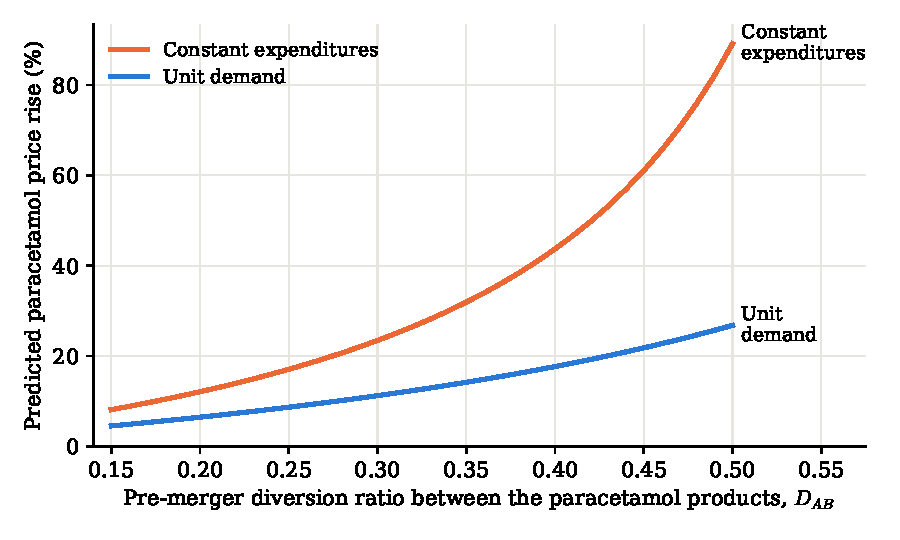
\includegraphics[width=0.78\textwidth]{figures/ch11/bv_curvature.pdf}
\caption{Predicted paracetamol price increase in the stylized calibration of \cref{tab:11-bvcurv}, against the
pre-merger diversion ratio between the two paracetamol products. Both versions match the same own elasticity
($-3$), diversion ratio and margins. The constant-expenditure version predicts 1.8 to 3.3 times the increase of
the unit-demand version.}
\label{fig:11-bvcurv}
\end{figure}

\Cref{tab:11-bvcurv} and \cref{fig:11-bvcurv} show the result. With identical first-order information the
constant-expenditure version predicts about twice the unit-demand increase at $D_{AB}=0.30$ and almost three times at
$D_{AB}=0.45$. Over the range shown the ratio lies between 1.8 and 3.3. Upward pricing pressure cannot distinguish
the two models, because it uses only first-order information. The simulation can, but only through an assumption
about curvature that pre-merger data barely constrain. The calibration also reproduces the second pattern of
Table 6. Rival price effects are below 1\% in both versions, because nested logit with substance nests diverts little
demand from paracetamol to each rival substance.

\casehead{Robustness} The working paper reports sensitivity checks run during and after the review
\citep[Sections 4.1 and 4.2]{BjornerstedtVerboven2013}. A potential market of 1.5, 4 or 6 times average sales, in
place of 2, gave similar results. A coarser product definition, with about 20 brand-form products per month instead
of 43, gave comparable findings. The full sample of 11,185 product-months gave the same conclusions as the
estimation sample. Adding sums of the pack sizes and doses of other products to the instruments left the unit-demand
results unchanged. Under constant expenditures it raised the elasticities and lowered the predicted price effects
somewhat, without changing the qualitative conclusions. Treating marketing as endogenous gave closely comparable
results. The reverse nesting order was rejected, as noted above.

\casehead{Interpretation} The study delivers three lessons. First, the constant-expenditure nested logit got the size
of the merging firms' price increase about right. It did so in the prediction made during the review, before the
outcome was known, and again in the published re-estimation. Second, the choice between specifications that fit the pre-merger data comparably
matters as much as the estimation itself. The unit-demand specifications implied implausibly elastic demand and low
margins, and they under-predicted the price increase by half or more. Third, the models missed how the effects were
distributed. They predicted very different increases for the two merging firms and small rival responses. The data
show similar increases for the two merging firms and increases of about 10 percent for some rivals.

Several explanations are possible. After the merger the merged firm cut its pack sizes from 30 to 20 tablets, as the
Swedish Medical Products Agency required. It lowered pack prices only slightly, for example from 41.5 to 38.5 kronor
for one of its best-selling products. The firms attributed the higher price per tablet to the cost of smaller packs. The authors
find this implausible, because ASA producers faced the same requirement without increases of similar size. The same
requirement may explain part of the ASA increase \citep[p.~29]{BjornerstedtVerboven2013}. The published version
considers a plausible post-merger cost increase and partial collusion as supply-side explanations
\citep[abstract]{BjornerstedtVerboven2016}. Rivals may have coordinated on higher prices after the merger, a
coordinated effect that a Bertrand model rules out (\cref{sec:11-millercoors}). The deregulation of pharmacies also
changed retail conditions in the same period. Finally, GSK was the acquirer and may have favored its own brands
after the merger. That would fit the small loss in its share (p.~32).

\casehead{Critiques and related validation studies} A single merger is a small sample for grading a method. The
retrospective benchmark rests on before-after comparisons of product-group prices, with rival controls whose prices
themselves moved. The change in pack sizes at the time of the merger further complicates the comparison of prices per
tablet. The predictions condition on the demand model's nest structure, which fixes how much substitution toward
rival substances is possible. Simulations that impose small cross-substance diversion will under-predict rivals'
responses whatever the curvature. \citet[p.~231]{AskerNocke2021} list four studies that grade merger simulations
with ex post evaluations: \citet{Peters2006}, \citet{Weinberg2011}, \citet{WeinbergHosken2013} and the present paper.
They reach mixed conclusions. \citet[pp.~627--628]{Peters2006} simulates five airline mergers completed between
August 1986 and November 1987. Standard simulations do not generally forecast the observed fare changes accurately.
Unobserved supply-side changes account for most of the gap in almost every case (p.~645). Peters concludes that
departures from the assumed model of conduct play an important role. \citet[p.~1584]{WeinbergHosken2013} simulate
two of the mergers of \cref{sec:11-ah}, Pennzoil and Quaker State in motor oil and Aurora and Log Cabin in syrup. For
motor oil the simulated increases are typically below 5 percent, against direct estimates of 4 to 8 percent. For
syrup the simulations typically predict 5 to 20 percent, while the merger had little effect on consumer prices.
\citet{AshenfelterHosken2010} find that the cereal simulation of \citet{Nevo2000b} predicted the wrong products to
rise in price (\cref{sec:11-ah}). \citet{Houde2012} compares a spatial simulation with a DiD estimate of the same
gasoline transaction (\cref{sec:11-beyond}).

\casehead{Contribution} The paper is one of the few direct tests of merger simulation as used by competition
authorities. It shows that simulations can predict the main effect of a merger when demand curvature is allowed to
be realistic. It also introduced the constant-expenditure nested logit, a tractable alternative to unit demand for
frequently purchased goods. Unit demand, the common default in discrete-choice models, can lead to large under-predictions even
when the model fits the pre-merger data. Retrospectives such as those in \cref{sec:11-retro} are therefore part of
the toolkit for choosing among prospective models.

\section{Coordinated effects: the MillerCoors joint venture}\label{sec:11-millercoors}

The merger analysis of \cref{sec:11-upp,sec:11-simulation} holds the mode of competition fixed. The merged firm
internalizes the competition among its own products, and every firm continues to set prices as a static
Bertrand-Nash player. Antitrust agencies worry about a second channel as well. The introduction to this chapter
distinguished the two channels informally, and we now state the distinction precisely.

\begin{definition}[Unilateral and coordinated effects]\label{def:11-coordinated}
A merger has \emph{unilateral effects} when it changes prices because the merged firm internalizes the competition
among the products it now owns. All firms keep playing the same static Nash equilibrium. A merger has
\emph{coordinated effects} when it also changes conduct, so that the merged firm and its remaining rivals compete
less aggressively with one another than static Nash pricing implies.
\end{definition}

\citet[p.~238]{AskerNocke2021} make the definition operational. A merger has coordinated effects when it leads to
prices that differ from those of a static Nash equilibrium. Any model of such effects therefore needs a continuation
value, which usually takes the defect-and-punish form of the collusion models of \cref{ch:collusion-theory}. The
idea is old. In the words of \citet{Stigler1964}, ``[c]ollusion of firms can take many forms, of which the most
comprehensive is outright merger''.
Section 7.2 of the 2010 Horizontal Merger
Guidelines discusses the market conditions that facilitate collusion \citep{USDOJFTC2010}, as \citet[p.~203,
n.~67]{AskerNocke2021} note. Merger challenges invoke coordinated effects often. Richard Gilbert and Hillary Greene
counted the merger complaints filed by the DOJ and the FTC between 1990 and 2014. In their count, as cited by
\citet{MillerWeinberg2017}, 60 percent alleged coordinated effects of some form \citep[p.~238,
n.~154]{AskerNocke2021}. Economists, by contrast, have concentrated on unilateral effects since the
1980s. Asker and Nocke attribute the focus to the analytical clarity of unilateral effects and to the lack of clear
empirical examples that link mergers to more coordination (pp.~238--239). \Cref{sec:11-ce-theory} sets out what the
theory says, and the rest of the section studies one of the few empirical examples.

\citet{MillerWeinberg2017} provide one of the first structural estimates of the coordinated effects of a consummated
merger.
They study the 2008 joint venture that combined the US brewing operations of SABMiller and Molson Coors into a new
firm, MillerCoors. Their method nests static Bertrand-Nash pricing inside a model in which the merged firm and its
largest rival put a weight $\kappa$ on each other's profits. It then estimates $\kappa$ from the post-merger prices.
This section follows the paper from its question to its contribution. It derives every estimating equation, proves
the properties of the estimator that the paper relies on, and reproduces Tables IV, V, VI and X.\footnote{Page
numbers in this section refer to the journal article. We change three pieces of the paper's notation to keep the
book consistent. The paper's nesting parameter $\rho$ is our $\sigma$ (in this book $\rho$ is pass-through). Its
product, period and region effects $\sigma_j$, $\tau_t$ and $\mu_r$ are our $\varphi_j$, $\tau_t$ and $\upsilon_r$.
The paper writes utility as $+\alpha p$ with $\alpha < 0$, while we write $-\alpha p$ with $\alpha > 0$. The tables
keep the paper's signs.}

\subsection{The theory of coordinated effects}\label{sec:11-ce-theory}

The theory of coordinated effects comes from the repeated games of \cref{ch:collusion-theory}. The question is
whether a change in market structure makes collusion easier to sustain, in the sense that it lowers the critical
discount factor above which collusion is an equilibrium. We follow \citet[pp.~239--240]{AskerNocke2021}, first in
the symmetric benchmark and then with capacities.

\casehead{Symmetric Bertrand competition}
Let $N$ symmetric firms sell a homogeneous good at constant marginal cost and set prices in every period of an
infinitely repeated game with discount factor $\delta$. Suppose all firms charge the monopoly price $p^m$ and share
the monopoly profit $\pi^m$ equally, and any deviation triggers static Bertrand pricing at marginal cost forever. A
firm that undercuts slightly takes the whole market for one period and earns close to $\pi^m$, and zero thereafter.
Collusion is an equilibrium if and only if
\begin{equation*}
\frac{1}{1 - \delta}\cdot\frac{\pi^m}{N} \ge \pi^m
\quad\Longleftrightarrow\quad
1 \ge N(1 - \delta)
\quad\Longleftrightarrow\quad
\delta \ge \underline\delta_N = 1 - \frac{1}{N} .
\end{equation*}
A merger from $N$ to $N - 1$ firms lowers the critical discount factor from $1 - \frac{1}{N}$ to $1 - \frac{1}{N -
1}$, so collusion becomes sustainable for more discount factors. Under imperfect monitoring, the time the industry
spends in the collusive state also falls with $N$. On this account, mergers facilitate collusion.

The model is special, because neither the deviation profit ($\pi^m$) nor the punishment profit (zero) depends on
$N$. In richer models both can fall with the number of firms. A merger then raises both the gain from cooperating
and the gain from deviating, and its effect on the critical discount factor is ambiguous. Firms also differ, and a
merger does more than remove a competitor, since the merged firm obtains the partners' tangible and intangible
assets.

\casehead{Capacity constraints}
\citet{CompteJennyRey2002} show how asymmetries change the answer. Demand is one unit at any price up to the monopoly
price of one, and zero above it. Firm $i$ has zero marginal cost up to its capacity $k_i$, with $k_1 \le k_2 \le
\dots \le k_N$. Write $\hat k_i = \min\{k_i, 1\}$ for firm $i$'s \emph{effective capacity}, $\hat K = \sum_i\hat k_i$
for the sum of effective capacities, and $K_{-N} = \sum_{i < N}k_i$ for the capacity of all firms but the largest.
Monitoring is perfect, and attention is restricted to equilibria in which each firm keeps the same market share
$\omega_i$ along every continuation path.
A merger of firms $l$ and $m$ combines their capacities into $k_l + k_m$
and creates no efficiencies.

\begin{proposition}[Capacities and collusion, \citealp{CompteJennyRey2002}]\label{prop:11-cjr}
\leavevmode
\begin{enumerate}[label=(\alph*)]
\item If $K_{-N} \ge 1$, perfect collusion at price one is sustainable if and only if
$\delta \ge \underline\delta = \frac{\hat K - 1}{\hat K}$, and the best shares are $\omega_i = \frac{\hat
k_i}{\hat K}$. If $K_{-N} \ge 1$ holds before and after a merger of $l$ and $m$, the merger weakly lowers
$\underline\delta$, and strictly if and only if $k_l + k_m > 1$.
\item If $K_{-N} < 1$, the largest firm's incentive constraint binds under the best allocation of shares, and
$\underline\delta = \frac{\hat k_N}{\hat K}$. A merger involving the largest firm raises $\underline\delta$. A
merger that does not involve the largest firm and does not create a new largest firm leaves it unchanged.
\end{enumerate}
\end{proposition}

\begin{proof}[Proof of part (a)]
Every firm's rivals together have capacity at least $K_{-N} \ge 1$, so they can serve the whole market. In the
static game the price is therefore zero and every firm earns zero, which is the harshest possible punishment. Under
collusion firm $i$ earns $\omega_i$ per period. Its best deviation prices just below one and sells $\hat k_i$, and it
earns zero afterward. It does not deviate if and only if
\begin{equation*}
\frac{\omega_i}{1 - \delta} \ge \hat k_i
\quad\Longleftrightarrow\quad
\delta \ge 1 - \frac{\omega_i}{\hat k_i} .
\end{equation*}
Collusion is sustainable if and only if $\delta \ge \max_i\big(1 - \frac{\omega_i}{\hat k_i}\big)$, so the best
shares maximize $\min_i\frac{\omega_i}{\hat k_i}$ subject to $\sum_i\omega_i = 1$. Because $\sum_i\hat
k_i\cdot\frac{\omega_i}{\hat k_i} = 1$, a weighted average of the ratios $\frac{\omega_i}{\hat k_i}$ with weights
$\frac{\hat k_i}{\hat K}$ equals $\frac{1}{\hat K}$. Their minimum is therefore at most $\frac{1}{\hat K}$, with
equality when every ratio equals $\frac{1}{\hat K}$. Hence $\underline\delta = 1 - \frac{1}{\hat K}$. A merger
replaces $\hat k_l + \hat k_m$ by $\min\{k_l + k_m, 1\}$, which is never larger and is strictly smaller if and only if
$k_l + k_m > 1$. A smaller $\hat K$ lowers $1 - \frac{1}{\hat K}$.
\end{proof}

Part (b) requires optimal punishments with two phases, a low price in the first period of the punishment and a high
price afterward. Static Nash pricing no longer holds the firms to their minmax payoffs
\citep[p.~240, n.~156]{AskerNocke2021}. We state part (b) without proof. The two parts reverse the symmetric intuition in
different ways. In part (a) a merger helps collusion only by destroying effective capacity. In part (b) a merger
that makes the largest firm larger makes the industry more asymmetric and hurts collusion. With capacities $(0.2,
0.3, 0.4, 1.0)$, for example, $K_{-N} = 0.9$ and $\underline\delta = \frac{1}{1.9} \approx 0.53$. A merger of the
largest firm with the smallest gives $(0.3, 0.4, 1.2)$ and $\underline\delta = \frac{1}{1.7} \approx 0.59$. A merger
of the two smallest gives $(0.4, 0.5, 1.0)$ and leaves $\underline\delta$ at 0.53.

\casehead{What the theory can and cannot say}
In a model with heterogeneous firms, a merger may thus help or hinder collusion, depending on the market and the
merger. Outside very special models the conditions are not well understood, and the theory gives no robust mapping
from a critical discount factor to the probability that collusion occurs \citep[p.~240]{AskerNocke2021}.
\citet{KaplowShapiro2007} put the problem sharply. Supergame theory with patient players predicts collusion for
almost any market structure, so it ``proves too much'' (n.~159). It is not surprising that courts in the last twenty
years have been reluctant to block mergers on coordinated-effects grounds, unless the industry had been cartelized
before. Conversely, a merger in an industry that is already cartelized may do little harm, and its efficiencies may
benefit society. \citet{RollerSteen2006} study a cartel in the Norwegian cement industry between 1955 and 1968. It
allocated market shares by capacity, which led to overinvestment in capacity. The 1968 merger of the industry's two
firms solved the coordination problem and removed the incentive to overinvest. Relative to wasteful collusion, this
merger to monopoly raised welfare, although competition would have raised it more (n.~160). Recent research gives
the concern a firmer empirical basis, and \citet{MillerWeinberg2017} is its leading example (p.~240).

\subsection{The question}\label{sec:11-mc-question}

The economic question is why the prices of the largest domestic beers rose after the joint venture, and whether the
rise reflects a change in how the remaining brewers compete. The joint venture combined the second and third largest
US brewers. A standard merger simulation predicts that the merged firm raises its prices, that rivals raise theirs a
little through strategic complementarity, and that efficiencies push in the other direction. The data show something
the standard model struggles to produce. The price of Bud Light, the flagship of the largest rival, rose by about as
much as the prices of Miller Lite and Coors Light. The prices of the leading imports did not rise.

The question matters for three reasons. First, it tests the maintained assumption of every merger simulation in
\cref{sec:11-simulation}, namely that post-merger conduct is static Nash. Second, it separates three forces that
act on post-merger prices at the same time: unilateral effects, coordinated effects and cost efficiencies. Third,
the US Department of Justice (DOJ) cleared the joint venture on the strength of its expected efficiencies. The
paper can ask whether that decision was right under different welfare standards.

The answer has three parts \citep[pp.~1781 and 1788]{MillerWeinberg2017}. The estimated internalization parameter is
between 0.25 and 0.37 and is significantly different from zero, so post-merger Nash-Bertrand pricing is rejected.
The joint venture produced large marginal-cost savings for MillerCoors, which roughly offset its unilateral effects.
Coordination raised the prices of all three domestic brewers well above their no-merger levels, so consumers lost
while total surplus rose slightly.

\subsection{The industry and the event}\label{sec:11-mc-industry}

The US beer market has many brands but few large brewers. Around the time of the joint venture, five firms
controlled about 80 percent of US retail revenue. Anheuser-Busch InBev (ABI), the owner of Budweiser and Bud Light, was the largest, with
about 35 percent. SABMiller (Miller) and Molson Coors (Coors) were the next two. Grupo Modelo (Corona) and Heineken
together held about 15 percent. Real beer prices fell between 2000 and 2008. \Cref{tab:11-mw-brands} lists the 13
brands in the paper's sample by owner.

\begin{table}[htbp]
\centering
\caption{Brewers and brands in the Miller and Weinberg sample}
\label{tab:11-mw-brands}
\footnotesize
\begin{tabular}{@{}lll@{}}
\toprule
Brewer (after June 2008) & Brands (row number in \cref{tab:11-mw-elast}) & Origin \\
\midrule
ABI & Bud Light (1), Budweiser (2), Michelob (9), Michelob Light (10) & Domestic \\
MillerCoors: Coors brands & Coors (3), Coors Light (4) & Domestic \\
MillerCoors: Miller brands & Miller Genuine Draft (11), Miller High Life (12), Miller Lite (13) & Domestic \\
Modelo & Corona Extra (5), Corona Light (6) & Imported \\
Heineken & Heineken (7), Heineken Light (8) & Imported \\
\bottomrule
\end{tabular}

\smallskip
\begin{minipage}{0.95\linewidth}
\footnotesize Notes: Each brand is sold in 6, 12 and 24 packs, and a product is a brand and package size. Before June
2008 the Miller and Coors brands belonged to separate firms. The brand list is the row list of
\citet[Table V]{MillerWeinberg2017}. Ownership is as described in the text.
\end{minipage}
\end{table}

The joint venture was announced on October 9, 2007 \citep[p.~9]{AshenfelterHoskenWeinberg2015} and consummated in June 2008
\citep[p.~1768]{MillerWeinberg2017}.
It combined the US operations of SABMiller and Molson Coors, with a combined share of about 30 percent. The DOJ
reviewed it as a merger and approved it on June 5, 2008. It found that efficiencies from combining the brewing
operations would outweigh any adverse competitive effect \citep[p.~241, n.~161]{AskerNocke2021}. The savings were in
shipping and distribution. Coors brewed in two locations and Miller in six. Moving Coors production into Miller
plants let the venture brew beer closer to many of its 48 regional markets \citep[pp.~219--220]{AskerNocke2021}. The
same investigation also surfaced documents that pointed to leader-follower pricing in the industry (p.~241).
\citet[p.~1788]{MillerWeinberg2017} consider a scenario with unilateral effects and efficiencies but no
coordination. They describe it as the one ``deemed most likely by the DOJ in its decision to clear the merger.''

Three institutional features matter for what follows. First, US beer is sold through a \emph{three-tier system}:
brewers sell to independent distributors, who sell to retailers. The model of the paper lets brewers sell directly
to consumers and treats the retail sector in a supplemental appendix \citep[p.~1779]{MillerWeinberg2017}. Second,
InBev acquired Anheuser-Busch in November 2008, five months after the joint venture \citep[p.~1784]{MillerWeinberg2017}.
Third, Anheuser-Busch held a large equity stake in Grupo Modelo during the sample period. \Cref{fig:11-beer} records it
as 50.3 percent before ABI bought the rest of Modelo in a \$20.1 billion deal. That acquisition came in 2013, after the
sample period \citep[p.~1767]{MillerWeinberg2017}. The second and third facts reappear in the assessment in
\cref{sec:11-mc-assessment}.

\subsection{Facts and hypotheses}\label{sec:11-mc-facts}

\Cref{fig:11-mwfacts} reproduces the paper's Figure 1. It plots the average log real price of a 12 pack of five
flagship brands from 2001 to 2011, in 2010 dollars. Before the joint venture, Miller Lite, Coors Light and Bud Light
move almost in lockstep and drift down. After June 2008 all three jump by roughly 6 log points and stay at the higher
level through 2011.\footnote{The 6 log point jump is our reading of the figure, from about 2.25--2.27 before June
2008 to about 2.29--2.33 afterwards. \citet[p.~242]{AskerNocke2021}, who reproduce the figure, describe the jump as
an 8 percent increase in the prices of all three brands. The paper itself states an increase of about 8 percent
\citep[p.~1768]{MillerWeinberg2017}, so we report both. The paper notes the brief dip in Miller Lite prices just
after the merger in its footnote 5.} Corona Extra and Heineken keep falling. In the paper's words, the imports ``do not exhibit any
persistent increase and instead continue along a downward trend'' \citep[p.~1769]{MillerWeinberg2017}. The price
gap between domestic beers and imports therefore shrinks.

\begin{figure}[htbp]
\centering
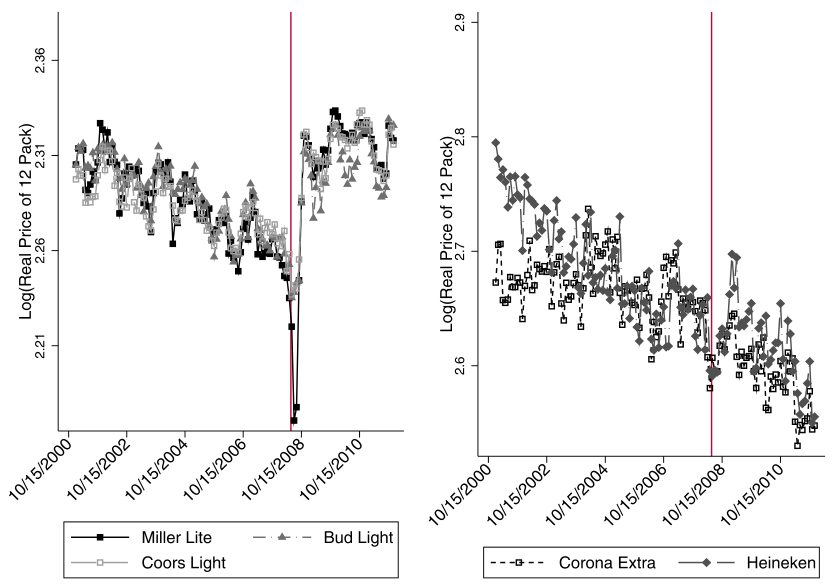
\includegraphics[width=0.92\textwidth]{figures/ch11/mw_fig1_prices.png}
\caption{Average retail prices of flagship 12 packs, 2001--2011. The left panel shows Miller Lite, Bud Light and Coors
Light, and the right panel shows Corona Extra and Heineken. The vertical axis is the natural log of the price in real
2010 dollars, and the vertical line marks the consummation of the joint venture in June 2008. Source: Miller and
Weinberg (2017), Figure 1.}
\label{fig:11-mwfacts}
\end{figure}

\citet[p.~1769]{MillerWeinberg2017} single out two features of the figure. The price of Bud Light rises by roughly
the same amount as the prices of Miller Lite and Coors Light. The prices of the Modelo and Heineken brands do not
rise, at least not persistently. They list four explanations that are consistent with these facts.
\begin{enumerate}[label=(H\arabic*)]
\item ABI and MillerCoors \emph{coordinate} after the merger and compete less aggressively with each other.
\item \emph{Unilateral effects} alone explain the data. Demand could make domestic beer prices strong strategic
complements of one another and weak strategic complements of import prices. Then ABI would follow MillerCoors up even
under Nash pricing, while importers would not.
\item \emph{Institutional practices} explain the data. Retailers might price Bud Light, Miller Lite and Coors Light
equally whatever happens to costs and demand, out of habit or under pressure from brewers.
\item The \emph{Great Recession} explains the data. The recession began at about the time of the merger. Lower incomes
could make domestic beer demand less elastic, for example through down-market substitution from imports.
\end{enumerate}
The paper weighs (H4) with a fact. Sales of the domestic brands fell in both absolute and relative terms during the
recession, which is hard to square with consumers trading down to them \citep[n.~5]{MillerWeinberg2017}.

The test the paper builds follows from (H1) and (H2). If unilateral effects alone explain the data, an estimated
demand system plus Nash pricing should reproduce the post-merger price of Bud Light. If they cannot, a model with
partial internalization of the ABI-MillerCoors pricing externality should fit better. The test therefore requires a
demand system rich enough to give (H2) a fair chance, and a supply model in which Nash pricing is a special case. The
logic is the same as in the conduct-parameter literature of \cref{ch:conduct}. The new element is a change in conduct
at a known date, caused by a known change in market structure.

\subsection{Theory: partial internalization of pricing externalities}\label{sec:11-mc-theory}

We first develop the supply model in general form. Consider one market and drop the region and period indices. There
are $J$ products and $F$ firms, and firm $f$ sells the products in $\mathcal{J}_f$. Market size is $M$, the share of
product $j$ is $s_j(p)$, marginal cost $mc_j$ is constant, and firm $f$'s variable profit is
\begin{equation}\label{eq:11-mc-profit}
  \pi_f(p) = M\sum_{k \in \mathcal{J}_f}(p_k - mc_k)\, s_k(p).
\end{equation}

\begin{assumption}[Partial internalization]\label{ass:11-mc-kappa}
(i) Firm $f$ chooses the prices of its products to maximize
\begin{equation}\label{eq:11-mc-objective}
  V_f(p) = \pi_f(p) + \sum_{g \neq f}\kappa_{fg}\,\pi_g(p),
\end{equation}
taking the prices of other firms as given, with weights $\kappa_{fg} \in [0,1]$ and $\kappa_{fg} = \kappa_{gf}$.
(ii) A Nash equilibrium of the game with payoffs $V_f$ exists and is interior.
\end{assumption}

\Cref{sec:11-simframework} stated the resulting first-order conditions without proof, and the worked example of
\cref{sec:11-logitex} used them. The weight $\kappa_{fg}$ is the fraction of rival $g$'s profit that firm $f$ counts
as its own. With all weights
equal to zero, the model is the multiproduct Bertrand-Nash model of \cref{ch:diffprod}. With $\kappa_{fg} = 1$, firms
$f$ and $g$ maximize their joint profit, exactly as if they had merged. Intermediate weights have two readings. The
first is literal: if firm $f$ owns a share of firm $g$'s equity, its owners gain from $g$'s profit
\citep{OBrienSalop2000}. The second is a reduced form for tacit coordination, which is the reading
\citet[p.~1779]{MillerWeinberg2017} adopt. They call $\kappa$ the ``post-merger internalization of coalition pricing
externalities.''

\begin{proposition}[First-order conditions with partial internalization]\label{prop:11-mc-foc}
Let $\Delta$ be the $J \times J$ matrix with $(j,k)$ element $\frac{\partial s_j}{\partial p_k}$, and let $\Omega(\kappa)$
be the matrix with $(j,k)$ element $\kappa_{f(j)f(k)}$, where $f(j)$ is the owner of product $j$ and $\kappa_{ff} = 1$.
Under \cref{ass:11-mc-kappa} equilibrium prices satisfy
\begin{equation}\label{eq:11-mc-foc}
  s(p) + \big(\Omega(\kappa) \odot \Delta(p)^\top\big)(p - mc) = 0 ,
\end{equation}
and, when the matrix is invertible, the markup vector is
\begin{equation}\label{eq:11-mc-markup}
  p - mc = b(p;\kappa) \equiv -\big[(\Omega(\kappa) \odot \Delta(p))^\top\big]^{-1} s(p).
\end{equation}
\end{proposition}

\begin{proof}
Take $j \in \mathcal{J}_f$. Differentiating \eqref{eq:11-mc-objective} with \eqref{eq:11-mc-profit} gives
\begin{align*}
  \frac{\partial V_f}{\partial p_j}
  &= M\Big[s_j + \sum_{k \in \mathcal{J}_f}(p_k - mc_k)\frac{\partial s_k}{\partial p_j}\Big]
     + \sum_{g \neq f}\kappa_{fg}\, M\sum_{k \in \mathcal{J}_g}(p_k - mc_k)\frac{\partial s_k}{\partial p_j} \\
  &= M\Big[s_j + \sum_{k=1}^{J}\kappa_{f(j)f(k)}\,(p_k - mc_k)\,\Delta_{kj}\Big].
\end{align*}
The second line uses $\kappa_{ff} = 1$ and collects all products into one sum. Setting the derivative to zero and
dividing by $M > 0$ gives $s_j + \sum_k \Omega_{jk}(\Delta^\top)_{jk}(p_k - mc_k) = 0$ for every $j$. Stacking the $J$
equations gives \eqref{eq:11-mc-foc}. Symmetry of the weights makes $\Omega(\kappa)$ symmetric, so
$\Omega \odot \Delta^\top = (\Omega \odot \Delta)^\top$, and solving for $p - mc$ gives \eqref{eq:11-mc-markup}.
\end{proof}

Equation \eqref{eq:11-mc-markup} is the markup formula of \cref{ch:blp} (\cref{eq:08-markup}) with the ownership
matrix replaced by $\Omega(\kappa)$. \citet[eq.~(9)]{MillerWeinberg2017} write it as
$p_t = mc_t - [\Omega_t(\kappa) \circ (\frac{\partial s_t}{\partial p_t})^\top]^{-1}s_t$, which is the same object.
In their application the weight is nonzero only for pairs of ABI and MillerCoors products after the merger. Let
$\mathcal{J}_A$, $\mathcal{J}_M$, $\mathcal{J}_O$ and $\mathcal{J}_H$ be the products of ABI, MillerCoors, Modelo and
Heineken, and write $\mathbf{1}$ for a matrix of ones of the conformable size. Ordering products by firm, the
post-merger matrix is
\begin{equation}\label{eq:11-mc-omega13}
  \Omega^{post}(\kappa) =
  \begin{bmatrix}
    \mathbf{1}_{AA} & \kappa\mathbf{1}_{AM} & 0 & 0 \\
    \kappa\mathbf{1}_{MA} & \mathbf{1}_{MM} & 0 & 0 \\
    0 & 0 & \mathbf{1}_{OO} & 0 \\
    0 & 0 & 0 & \mathbf{1}_{HH}
  \end{bmatrix}.
\end{equation}
Before the merger the Miller and Coors blocks are separate, so $\Omega^{pre}$ is block diagonal with five blocks.
The paper illustrates with a hypothetical region in which ABI, Miller, Coors and Modelo each sell one product
\citep[eq.~(10)]{MillerWeinberg2017}:
\begin{equation}\label{eq:11-mc-omega4}
  \Omega_{t_1^*} =
  \begin{bmatrix} 1 & 0 & 0 & 0 \\ 0 & 1 & 0 & 0 \\ 0 & 0 & 1 & 0 \\ 0 & 0 & 0 & 1 \end{bmatrix},
  \qquad
  \Omega_{t_2^*} =
  \begin{bmatrix} 1 & \kappa & \kappa & 0 \\ \kappa & 1 & 1 & 0 \\ \kappa & 1 & 1 & 0 \\ 0 & 0 & 0 & 1 \end{bmatrix},
\end{equation}
where $t_1^*$ is a pre-merger period and $t_2^*$ a post-merger period. Miller and Coors fully internalize each other
after the merger, ABI and MillerCoors internalize each other with weight $\kappa$, and Modelo prices as a Nash
player. The last feature is a restriction. The paper imposes it for Modelo and Heineken on the basis of qualitative
evidence \citep[p.~1779]{MillerWeinberg2017}.

\begin{remark}[$\kappa$ and the conduct parameter]\label{rem:11-mc-theta}
In a homogeneous-good market with $N$ symmetric firms, constant marginal cost $c$ and inverse demand $P(Q)$, let each
firm maximize $\pi_i + \kappa\sum_{j \neq i}\pi_j$ over its output. The first-order condition is
\begin{equation*}
  P(Q) + q_i P'(Q) - c + \kappa P'(Q)\sum_{j \neq i}q_j = 0 .
\end{equation*}
At a symmetric equilibrium $q_i = \frac{Q}{N}$ and $\sum_{j\neq i}q_j = \frac{(N-1)Q}{N}$, so
\begin{equation*}
  P(Q) - c + \theta\, Q P'(Q) = 0, \qquad \theta = \frac{1}{N} + \kappa\,\frac{N-1}{N}.
\end{equation*}
This is the conduct-parameter form of \cref{ch:conduct}. The weight $\kappa = 0$ gives Cournot ($\theta = \frac{1}{N}$)
and $\kappa = 1$ gives monopoly ($\theta = 1$). The internalization weight is thus a conduct parameter, and the
critique of \citet{Corts1999} applies to it. \Cref{sec:11-mc-assessment} returns to this point.
\end{remark}

The next result says how $\kappa$ changes pricing incentives at pre-merger prices. It extends the upward pricing
pressure (UPP) of \cref{sec:11-upp} to partial internalization. Write $D_{jk} = -\frac{\Delta_{kj}}{\Delta_{jj}}$
for the diversion ratio from $j$ to $k$ and $m_k = p_k - mc_k$ for the margin.

\begin{proposition}[Pricing pressure with partial internalization]\label{prop:11-mc-upp}
Suppose pre-merger prices satisfy \eqref{eq:11-mc-foc} with $\Omega^{pre}$, and evaluate the post-merger objectives at
pre-merger prices and costs. Then the post-merger pricing pressure on each product is:
\begin{align}
  \text{ABI product } j \in \mathcal{J}_A: &\quad UPP_j = \kappa\sum_{k \in \mathcal{J}_M} m_k D_{jk}, \label{eq:11-mc-upp-abi}\\
  \text{Miller product } j: &\quad UPP_j = \sum_{k \in \text{Coors}} m_k D_{jk} + \kappa\sum_{k \in \mathcal{J}_A} m_k D_{jk},
  \label{eq:11-mc-upp-mc}\\
  \text{import } j \in \mathcal{J}_O \cup \mathcal{J}_H: &\quad UPP_j = 0. \notag
\end{align}
The expression for a Coors product exchanges the roles of Miller and Coors in \eqref{eq:11-mc-upp-mc}.
\end{proposition}

\begin{proof}
Take $j \in \mathcal{J}_A$. At pre-merger prices the pre-merger condition holds:
$s_j + \sum_{k \in \mathcal{J}_A} m_k \Delta_{kj} = 0$. The post-merger derivative of $\frac{V_A}{M}$ with respect to
$p_j$ is the same expression plus $\kappa\sum_{k \in \mathcal{J}_M} m_k \Delta_{kj}$. At pre-merger prices it therefore
equals $\kappa\sum_{k\in\mathcal{J}_M} m_k\Delta_{kj}$. Dividing by $-\Delta_{jj} > 0$ converts it into dollars per
unit, as in \cref{sec:11-upp}:
\begin{equation*}
  \frac{\kappa\sum_{k\in\mathcal{J}_M} m_k\Delta_{kj}}{-\Delta_{jj}} = \kappa\sum_{k\in\mathcal{J}_M} m_k D_{jk}.
\end{equation*}
For a Miller product the post-merger objective adds the Coors products with weight one and the ABI products with
weight $\kappa$, and the same steps give \eqref{eq:11-mc-upp-mc}. Import objectives do not change.
\end{proof}

Under Nash pricing ($\kappa = 0$) ABI faces no direct pressure. Its prices rise only through strategic
complementarity, because MillerCoors's higher prices raise the demand for ABI's products. With $\kappa > 0$, ABI
faces pressure equal to $\kappa$ times the pressure it would face if it had merged with MillerCoors. This is the
sense in which coordination makes the largest rival behave like a partial merger partner. Efficiencies enter the
MillerCoors expressions as a credit $E_j mc_j$, exactly as in \cref{prop:11-netupp}.

Coordination also changes how rivals respond to the merged firm's efficiencies. In the Nash model a cost reduction at
MillerCoors lowers MillerCoors's prices, and strategic complementarity then lowers ABI's prices. With $\kappa > 0$
there is a countervailing force. A larger MillerCoors margin raises the value to ABI of the sales it diverts to
MillerCoors, so ABI wants to raise its price. \Cref{fig:11-mwident} shows the result in the logit illustration of
\cref{ex:11-logit}, which is also the example of \citet[p.~1780]{MillerWeinberg2017}. Three symmetric single-product
firms face logit demand with price 1.00, marginal cost 0.70, inside shares of 0.20 and an outside share of 0.40, and
firms 1 and 2 merge. At $\kappa = 0$ the rival price $p_3$ rises with the merged firm's cost $c_M$, with slope 0.061 at
$c_M = 0.6$. At $\kappa = 0.5$ the slope is $-0.148$.\footnote{These slopes and the contours in
\cref{fig:11-mwident} are our computations.} The figure also
previews the identification argument of \cref{sec:11-mc-supply}. The merging-firm price $p_M$ and the rival price
$p_3$ trace two families of curves that cross. An observed pair $(p_M, p_3)$ therefore pins down both the
internalization weight and the efficiency. For example, the pair $(1.09, 1.08)$ reported in the paper's third case
corresponds to $\kappa = 0.53$ and $c_M = 0.68$ in our computation (\cref{rem:11-mw-typo} discusses this case).

\begin{figure}[htbp]
\centering
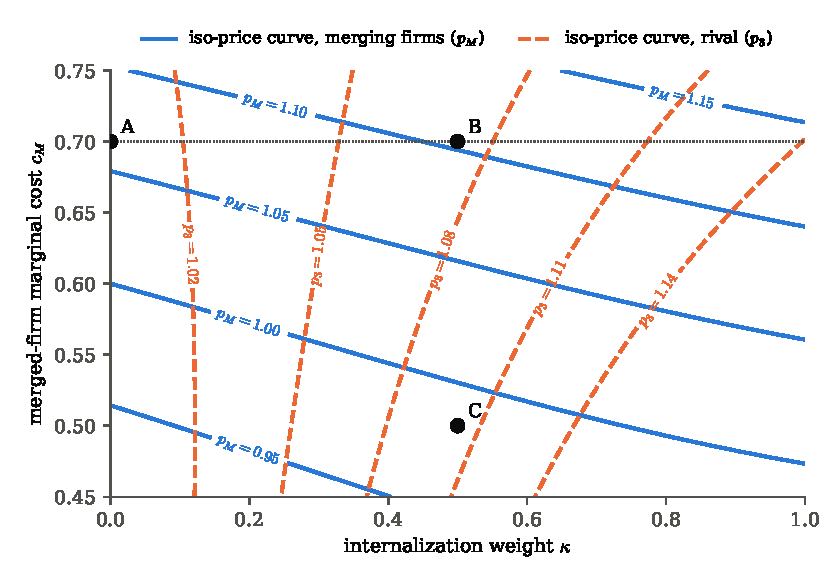
\includegraphics[width=0.82\textwidth]{figures/ch11/mw_identification.pdf}
\caption{Identification of the internalization weight and the efficiency in the logit illustration. Three symmetric
firms with logit demand start at price 1.00, marginal cost 0.70 and shares 0.20 (outside share 0.40). Firms 1 and 2
merge and both get marginal cost $c_M$, and the merged firm and firm 3 put weight $\kappa$ on each other's profits.
Solid curves are combinations of $(\kappa, c_M)$ that give the same merging-firm price $p_M$. Dashed curves give the
same rival price $p_3$. Point A is post-merger Nash pricing without efficiencies, $p = (1.064, 1.064, 1.006)$. Point B
has $\kappa = 0.5$, $p = (1.104, 1.104, 1.073)$. Point C has $\kappa = 0.5$ and $c_M = 0.5$, $p = (0.983, 0.983,
1.103)$. Our computations.}
\label{fig:11-mwident}
\end{figure}

\subsection{Data}\label{sec:11-mc-data}

The underlying data are weekly retail scanner data from supermarkets, collected by IRI
\citep[p.~241, n.~162]{AskerNocke2021}. The estimation samples aggregate them to months and quarters. A product $j$ is a brand and package size, with 13 brands sold in 6, 12 and 24 packs. A market is one of 39
geographic regions $r$ in one period $t$. The descriptive evidence spans 2001 to 2011. The estimation samples start in
2005, the first year of the household data described below \citep[p.~1768]{MillerWeinberg2017}. The baseline sample
has 94,656 brand-size-region-month observations, and a quarterly version has 31,784 brand-size-region-quarter
observations (Table IV notes). Both samples exclude the twelve months from June 2008 to May 2009, so the estimates compare settled pre-merger and
post-merger periods. Prices are in real 2010 dollars. Markups are reported on an ``equivalent-unit basis''
\citep[p.~1781]{MillerWeinberg2017}. The average markup of \$3.60 equals 34 percent of the retail price, which
implies an average price near \$10.60 per equivalent unit, close to the 12-pack prices in Table X.

Three further ingredients complete the data \citep[p.~1774]{MillerWeinberg2017}. Household incomes $D_i$ come from 500
draws per region and year from the American Community Survey (ACS), available for 2005 to 2011 (p.~1768). Market size $M_{rt}$ is set 50 percent above the maximum
unit sales observed in the region. The outside good collects brands outside the sample (such as craft beers), beer
sold outside supermarkets, and other beverages such as wine. Placing these products in the outside good makes their
prices non-strategic in the model. Period fixed effects absorb the trend toward craft beer. The cost side uses the
distance between each brand's brewery and each region, multiplied by an index of diesel prices
\citep[p.~1779]{MillerWeinberg2017}.

\subsection{Demand: the random coefficients nested logit}\label{sec:11-mc-demand}

\casehead{Utility}
Household $i$ in region $r$ and period $t$ chooses one of the inside products $j = 1, \dots, J_{rt}$ or the outside
good $j = 0$. There are two groups $g \in \{0, 1\}$: group 1 contains the inside goods and group 0 the outside good.
In book notation the indirect utility of an inside good is
\begin{align}
  u_{ijrt} &= \delta_{jrt} + \mu_{ijrt} + \zeta_{igrt} + (1-\sigma)\epsilon_{ijrt}, \label{eq:11-mc-utility}\\
  \delta_{jrt} &= x_j\beta - \alpha p_{jrt} + \varphi^D_j + \tau^D_t + \xi_{jrt}, \label{eq:11-mc-delta}\\
  \mu_{ijrt} &= \Pi_1 D_i\, p_{jrt} + D_i\, x_j\pi, \label{eq:11-mc-mu}
\end{align}
and $u_{i0rt} = \epsilon_{i0rt}$ \citep[eqs.~(4)--(5)]{MillerWeinberg2017}. The mean utility $\delta_{jrt}$ contains
product fixed effects $\varphi^D_j$, period fixed effects $\tau^D_t$ and the unobserved demand shock $\xi_{jrt}$.
Because the characteristics $x_j$ do not vary over time, $\varphi_j^D$ absorbs $x_j\beta$. The deviation $\mu_{ijrt}$
interacts income with price and with the characteristics $x_j = (1, \text{calories}_j, \text{import}_j,
\text{package size}_j)$, whose coefficients are $\pi = (\Pi_2, \Pi_3, \Pi_4, \Pi_5)^\top$. Household $i$'s price
coefficient is therefore
\begin{equation}\label{eq:11-mc-alphai}
  \alpha_i = \alpha - \Pi_1 D_i ,
\end{equation}
so a positive $\Pi_1$ means richer households are less price sensitive. The shock $\epsilon_{ijrt}$ is \iid\ type-I
extreme value. The group shock $\zeta_{igrt}$ has the distribution of \citet{Cardell1997}, which makes
$\zeta_{igrt} + (1-\sigma)\epsilon_{ijrt}$ extreme value. The \emph{nesting parameter} $\sigma \in [0,1)$ measures the
correlation of a household's tastes for inside goods. A larger $\sigma$ means less substitution between the inside
goods and the outside good.

The specification has two departures from the models of \cref{ch:logit,ch:blp}. Heterogeneity enters only through
observed income, with no unobserved random coefficients. This is the random coefficients nested logit (RCNL) of
\citet{BrenkersVerboven2006} and \citet{GrigolonVerboven2014}. The nest is a single inside-good group, with no
subnests for light beers, domestic beers or package sizes.

\casehead{The nested logit special case}
With $\Pi = 0$ the model is a one-level nested logit. We derive its shares and inversion, since the RCNL applies the
same algebra household by household. Drop the market subscripts, set $\delta_0 = 0$, and define the
\emph{inclusive value} of the inside group,
\begin{equation}\label{eq:11-mc-iv}
  I_1 = (1-\sigma)\ln\sum_{k=1}^{J}\exp\Big(\frac{\delta_k}{1-\sigma}\Big).
\end{equation}
The nested logit choice probabilities (\cref{ch:logit}) are
\begin{equation}\label{eq:11-mc-nlshares}
  s_{j|g} = \exp\Big(\frac{\delta_j - I_1}{1-\sigma}\Big), \qquad
  s_g = \frac{e^{I_1}}{1 + e^{I_1}}, \qquad
  s_0 = \frac{1}{1 + e^{I_1}}, \qquad
  s_j = s_{j|g}\, s_g ,
\end{equation}
where $s_{j|g}$ is the share of $j$ among inside goods and $s_g$ is the inside share.

\begin{proposition}[Nested logit inversion]\label{prop:11-mc-nlinv}
In the nested logit model,
\begin{equation}\label{eq:11-mc-nlinv}
  \ln s_j - \ln s_0 = \delta_j + \sigma\ln s_{j|g}.
\end{equation}
With \eqref{eq:11-mc-delta}, the estimating equation is
\begin{equation}\label{eq:11-mc-nlreg}
  \ln s_{jrt} - \ln s_{0rt} = -\alpha p_{jrt} + \sigma\ln s_{jrt|g} + \varphi^D_j + \tau^D_t + \xi_{jrt},
\end{equation}
which is the paper's equation (7) in book notation.
\end{proposition}

\begin{proof}
Take logs of $s_j = s_{j|g}s_g$ and use \eqref{eq:11-mc-nlshares}:
\begin{equation*}
  \ln s_j = \frac{\delta_j - I_1}{1-\sigma} + I_1 - \ln(1 + e^{I_1}), \qquad \ln s_0 = -\ln(1 + e^{I_1}).
\end{equation*}
Subtract the second equation from the first:
\begin{equation*}
  \ln s_j - \ln s_0 = \frac{\delta_j}{1-\sigma} - \frac{\sigma}{1-\sigma}I_1 .
\end{equation*}
The unobserved inclusive value can be eliminated with the within-group share. From \eqref{eq:11-mc-nlshares},
$\ln s_{j|g} = \frac{\delta_j - I_1}{1-\sigma}$, so $I_1 = \delta_j - (1-\sigma)\ln s_{j|g}$. Substituting,
\begin{equation*}
  \ln s_j - \ln s_0 = \frac{\delta_j}{1-\sigma} - \frac{\sigma\delta_j}{1-\sigma} + \sigma\ln s_{j|g}
  = \delta_j + \sigma\ln s_{j|g}.
\end{equation*}
Substituting \eqref{eq:11-mc-delta}, with $x_j\beta$ absorbed by $\varphi_j^D$, gives \eqref{eq:11-mc-nlreg}.
\end{proof}

Equation \eqref{eq:11-mc-nlreg} is linear in $(\alpha, \sigma)$ and the fixed effects. Both the price and the
within-group share are endogenous, since a high $\xi_{jrt}$ raises the product's share among inside goods and, through
the pricing equation, its price. Estimation therefore needs at least two excluded instruments. Column (i) of Table IV
estimates \eqref{eq:11-mc-nlreg} by two-stage least squares (\cref{cor:08-2sls}).

The nested logit derivatives follow from the same expressions, and they agree with \cref{lem:11-nl-deriv} for a
single inside nest. Using $\frac{\partial I_1}{\partial \delta_k} = s_{k|g}$ and $s_g s_{k|g} = s_k$,
\begin{equation*}
  \frac{\partial \ln s_j}{\partial \delta_k} = \frac{\indic\{j=k\} - s_{k|g}}{1-\sigma} + s_{k|g} - s_g s_{k|g}
  = \frac{\indic\{j=k\}}{1-\sigma} - \frac{\sigma}{1-\sigma}s_{k|g} - s_k .
\end{equation*}
Since $\frac{\partial\delta_k}{\partial p_k} = -\alpha$, the share derivatives are
\begin{equation}\label{eq:11-mc-nlderiv}
  \frac{\partial s_j}{\partial p_k} = -\alpha s_j\Big[\frac{\indic\{j=k\}}{1-\sigma} - \frac{\sigma}{1-\sigma}s_{k|g}
  - s_k\Big], \qquad \frac{\partial s_0}{\partial p_k} = \alpha s_0 s_k .
\end{equation}
The elasticities are
\begin{equation}\label{eq:11-mc-nlelast}
  \varepsilon_{jj} = -\alpha p_j\Big[\frac{1}{1-\sigma} - \frac{\sigma}{1-\sigma}s_{j|g} - s_j\Big], \qquad
  \varepsilon_{jk} = \alpha p_k\Big[\frac{\sigma}{1-\sigma}s_{k|g} + s_k\Big] \quad (k \neq j).
\end{equation}
The cross elasticity $\varepsilon_{jk}$ does not depend on $j$, so within the inside group substitution is
proportional to shares. This is the independence of irrelevant alternatives inside the nest. Dividing the cross
derivatives by the own derivative gives the diversion ratios
\begin{equation}\label{eq:11-mc-nldiv}
  D_{jk} = \frac{s_{k|g}\,[\sigma + (1-\sigma)s_g]}{1 - \sigma s_{j|g} - (1-\sigma)s_j}, \qquad
  D_{j0} = \frac{(1-\sigma)s_0}{1 - \sigma s_{j|g} - (1-\sigma)s_j}.
\end{equation}
The first expression is \eqref{eq:11-nl-diversion} with one inside nest, since $s_k = s_{k|g}s_g$. For small
products the outside diversion is close to $(1-\sigma)s_0$. A nesting parameter near one therefore sends
almost all of a product's lost sales to other beers.

\begin{remark}[Market elasticity, own elasticity and outside diversion]\label{rem:11-mc-identity}
When price enters utility linearly with a coefficient common to all products for each household, the matrix $\Delta$
is symmetric. This holds for the nested logit, by \eqref{eq:11-mc-nlderiv}, and for the RCNL below. Let all inside
prices rise by the same amount $\dd p$. Then
\begin{equation*}
  \dd s_j = \Big(\Delta_{jj} + \sum_{k\neq j}\Delta_{jk}\Big)\dd p = \Big(\Delta_{jj} + \sum_{k\neq j}\Delta_{kj}\Big)\dd p
  = \Delta_{jj}\Big(1 - \sum_{k\neq j}D_{jk}\Big)\dd p = \Delta_{jj}\, D_{j0}\, \dd p .
\end{equation*}
A uniform rise of $\dd p$ therefore changes the sales of product $j$ by $\varepsilon_{jj}D_{j0}\frac{\dd p}{p_j}$
percent. When prices are similar, the market elasticity is close to a share-weighted average of $\varepsilon_{jj}
D_{j0}$. Table IV satisfies this relation closely at the medians. For column (i), $-3.81 \times 0.298 = -1.14$ against a reported $-1.10$. For column
(ii), $-4.74 \times 0.1296 = -0.61$ against $-0.60$. Columns (iii) to (v) give $-0.74$, $-0.62$ and $-0.72$ against
$-0.72$, $-0.60$ and $-0.69$.
\end{remark}

\casehead{Market shares with random coefficients}
With $\Pi \neq 0$ the nested logit holds for each household. Let $V_{ijrt} = \delta_{jrt} + \mu_{ijrt}$ and define the
household's inclusive values
\begin{equation}\label{eq:11-mc-ivi}
  I_{i0rt} = 0, \qquad I_{i1rt} = (1-\sigma)\ln\sum_{k=1}^{J_{rt}}\exp\Big(\frac{V_{ikrt}}{1-\sigma}\Big), \qquad
  I_{irt} = \ln\big(1 + e^{I_{i1rt}}\big).
\end{equation}
Applying \eqref{eq:11-mc-nlshares} to household $i$ and averaging over the $N_{rt} = 500$ simulated households gives
\begin{equation}\label{eq:11-mc-rcnlshare}
  s_{jrt} = \frac{1}{N_{rt}}\sum_{i=1}^{N_{rt}}
  \underbrace{\frac{\exp\big(\frac{V_{ijrt}}{1-\sigma}\big)}{\exp\big(\frac{I_{i1rt}}{1-\sigma}\big)}}_{s_{ij|g}}\;
  \underbrace{\frac{\exp(I_{i1rt})}{\exp(I_{irt})}}_{s_{ig}},
\end{equation}
which is the paper's equation (6). The first fraction is the household's probability of choosing $j$ among inside
goods, because $\exp(\frac{I_{i1rt}}{1-\sigma}) = \sum_k \exp(\frac{V_{ikrt}}{1-\sigma})$. The second is its
probability of buying beer. These inclusive values are those of \citet{McFadden1978}. The household-level derivatives
follow from \eqref{eq:11-mc-nlderiv} with $\alpha_i$ in place of $\alpha$:
\begin{equation}\label{eq:11-mc-rcnlderiv}
  \Delta_{jk} = \frac{\partial s_j}{\partial p_k} = -\frac{1}{N}\sum_{i=1}^{N}\alpha_i\, s_{ij}
  \Big[\frac{\indic\{j=k\}}{1-\sigma} - \frac{\sigma}{1-\sigma}s_{ik|g} - s_{ik}\Big].
\end{equation}
Households differ in $\alpha_i$ and in their choice probabilities, so the aggregate cross elasticities depend on
which households buy which products. This breaks the proportional substitution of \eqref{eq:11-mc-nlelast}. Income
also shifts the attractiveness of beer and of particular characteristics, which lets the recession move demand.

\casehead{Inversion and the dampened contraction}
For trial values of the nonlinear parameters $\theta_2 = (\sigma, \Pi)$, the mean utilities $\delta_{rt}$ in each
market solve $s^{obs}_{rt} = s_{rt}(\delta_{rt};\theta_2)$. The BLP contraction of \cref{ch:blp} need not converge
in this model. The paper follows \citet{GrigolonVerboven2014}, who iterate
\begin{equation}\label{eq:11-mc-contraction}
  \delta^{h+1} = \Phi(\delta^h), \qquad \Phi(\delta) = \delta + (1-\sigma)\big[\ln s^{obs} - \ln s(\delta;\theta_2)\big].
\end{equation}
The factor $1-\sigma$ dampens each step (\cref{rem:08-rcnl}). The next result shows why it is needed and why it works.

\begin{proposition}[Dampened contraction in the RCNL]\label{prop:11-mc-contraction}
For every $\delta$, the Jacobian of $\Phi$ in \eqref{eq:11-mc-contraction} has strictly positive elements
\begin{equation}\label{eq:11-mc-phijac}
  \frac{\partial \Phi_j}{\partial \delta_k} = \frac{1}{s_j}\,\frac{1}{N}\sum_{i=1}^{N}s_{ij}\big[\sigma s_{ik|g} +
  (1-\sigma)s_{ik}\big],
\end{equation}
and its row sums equal
\begin{equation}\label{eq:11-mc-rowsum}
  \sum_{k}\frac{\partial \Phi_j}{\partial \delta_k} = 1 - (1-\sigma)\,\frac{1}{s_j}\,\frac{1}{N}\sum_{i=1}^{N}s_{ij}\,s_{i0} < 1 .
\end{equation}
Without dampening, the diagonal element of the Jacobian of $\delta + \ln s^{obs} - \ln s(\delta)$ is
$-\frac{\sigma}{1-\sigma}$ plus terms that vanish as the shares go to zero.
\end{proposition}

\begin{proof}
Differentiate \eqref{eq:11-mc-rcnlshare}. Household $i$'s nested logit gives
$\frac{\partial s_{ij}}{\partial \delta_k} = s_{ij}[\frac{\indic\{j=k\}}{1-\sigma} - \frac{\sigma}{1-\sigma}s_{ik|g}
- s_{ik}]$, as in the derivation of \eqref{eq:11-mc-nlderiv}. Hence
\begin{align*}
  (1-\sigma)\frac{\partial \ln s_j}{\partial \delta_k}
  &= \frac{1}{s_j}\frac{1}{N}\sum_i s_{ij}\big[\indic\{j=k\} - \sigma s_{ik|g} - (1-\sigma)s_{ik}\big] \\
  &= \indic\{j=k\} - \frac{1}{s_j}\frac{1}{N}\sum_i s_{ij}\big[\sigma s_{ik|g} + (1-\sigma)s_{ik}\big],
\end{align*}
where the second step uses $\frac{1}{N}\sum_i s_{ij} = s_j$. Since $\frac{\partial\Phi_j}{\partial\delta_k} =
\indic\{j=k\} - (1-\sigma)\frac{\partial\ln s_j}{\partial\delta_k}$, this gives \eqref{eq:11-mc-phijac}. Every term
is positive because all choice probabilities are positive. For the row sum, use $\sum_k s_{ik|g} = 1$ and $\sum_k
s_{ik} = 1 - s_{i0}$:
\begin{equation*}
  \sum_k\big[\sigma s_{ik|g} + (1-\sigma)s_{ik}\big] = \sigma + (1-\sigma)(1 - s_{i0}) = 1 - (1-\sigma)s_{i0}.
\end{equation*}
Averaging with weights $\frac{s_{ij}}{N s_j}$ gives \eqref{eq:11-mc-rowsum}. Without dampening the diagonal element is
$1 - \frac{\partial\ln s_j}{\partial\delta_j}$. The leading part of $\frac{\partial \ln s_j}{\partial\delta_j}$ is
$\frac{1}{1-\sigma}$, so the diagonal element is $1 - \frac{1}{1-\sigma} = -\frac{\sigma}{1-\sigma}$ plus terms
proportional to the shares.
\end{proof}

The sup norm of a matrix with nonnegative elements is its largest row sum, so \eqref{eq:11-mc-rowsum} makes $\Phi$ a
local contraction everywhere. The global argument then proceeds as for the BLP contraction in \cref{thm:08-contraction}.
Without dampening the map expands. At the paper's estimate $\sigma \approx 0.83$, the diagonal element is near
$-\frac{0.83}{0.17} \approx -4.9$, so plain iteration overshoots and diverges. The proposition also gives the speed of
convergence. The modulus is close to $1 - (1-\sigma)s_0$, so convergence slows as $\sigma$ approaches one. In the
plain nested logit the Jacobian elements are $\sigma s_{k|g} + (1-\sigma)s_k$, which are small when there are many
products.

\casehead{The GMM estimator}
The demand parameters are $\theta^D = (\alpha, \sigma, \Pi, \varphi^D, \tau^D)$. Given $\theta_2$, the inversion
delivers $\delta_{jrt}(\theta_2)$ and \eqref{eq:11-mc-delta} gives the structural error
\begin{equation}\label{eq:11-mc-xi}
  \xi_{jrt}(\theta^D) = \delta_{jrt}(\theta_2) + \alpha p_{jrt} - \varphi^D_j - \tau^D_t .
\end{equation}
With a vector of instruments $z_{jrt}$, the moment condition is $\E[z_{jrt}\,\xi_{jrt}(\theta^D_0)] = 0$, and the
estimator minimizes
\begin{equation}\label{eq:11-mc-gmm}
  \hat\theta^D = \argmin_{\theta^D}\; \xi(\theta^D)^\top Z\, W Z^\top \xi(\theta^D),
\end{equation}
where $Z$ stacks the instruments and $W$ is a weighting matrix. The parameters that enter linearly, $\alpha$ and the
fixed effects, are concentrated out by linear instrumental variables for each $\theta_2$ (\cref{prop:08-concentrate}),
so the nonlinear search runs over $(\sigma, \Pi)$ only. The paper uses two-stage least squares for the nested logit
and GMM for the four RCNL specifications. Standard errors are clustered by region (Table IV notes).

\casehead{Instruments and identification}
The paper uses five sets of excluded instruments. Each is excluded from \eqref{eq:11-mc-delta} and is meant to
move a particular endogenous object.
\begin{enumerate}[label=(\roman*)]
\item The distance between the brewery and the region, in miles times a diesel price index, shifts marginal cost
and hence price. Product fixed effects absorb a brand's average distance. Identification therefore comes from changes
in diesel prices and in shipping routes over time, including the post-merger reallocation of production.
\item A post-merger indicator interacted with $\indic\{j \in \mathcal{J}_A \cup \mathcal{J}_M\}$ shifts the markups
of ABI and MillerCoors through the change in ownership and conduct. The exclusion restriction requires that the merger
did not shift the unobserved demand for these brands relative to imports.
\item The number of products in the market, interacted with the same indicator, captures variation in the choice
set. It moves within-group shares and competitors' prices, and it identifies $\sigma$.
\item The sum of the distances of the products in the market, also interacted, collects rivals' cost shifters.
These move rivals' prices and hence $s_{j|g}$.
\item Mean regional income interacted with characteristics such as calories and import status varies across regions
and over time. This variation identifies $\Pi$.
\end{enumerate}
The logic matches \cref{sec:08-instruments}. Price needs a cost shifter or a markup shifter. The nesting parameter
needs variation in the within-group share that is unrelated to $\xi$, which choice-set variation provides. The
income interactions need variation in the distribution of $D_i$ across markets.

\casehead{Results}
\Cref{tab:11-mw-demand} reproduces Table IV. All five specifications include product and period fixed effects.
Column (i) is the nested logit, and columns (ii) to (v) are RCNL specifications on monthly or quarterly data that
differ in which income interactions they include.

\begin{table}[htbp]
\centering
\caption{Baseline demand estimates (Miller and Weinberg 2017, Table IV)}
\label{tab:11-mw-demand}
\footnotesize
\begin{tabular}{@{}llccccc@{}}
\toprule
Demand model & & NL-1 & RCNL-1 & RCNL-2 & RCNL-3 & RCNL-4 \\
Data frequency & & Monthly & Monthly & Quarterly & Monthly & Quarterly \\
Variable & Parameter & (i) & (ii) & (iii) & (iv) & (v) \\
\midrule
Price & $\alpha$ & $-0.1312$ & $-0.0887$ & $-0.1087$ & $-0.0798$ & $-0.0944$ \\
 & & (0.0884) & (0.0141) & (0.0163) & (0.0147) & (0.0146) \\
Nesting parameter & $\sigma$ & 0.6299 & 0.8299 & 0.7779 & 0.8079 & 0.8344 \\
 & & (0.0941) & (0.0402) & (0.0479) & (0.0602) & (0.0519) \\
\addlinespace
\multicolumn{7}{@{}l}{\textit{Demographic interactions}} \\
Income $\times$ price & $\Pi_1$ & & 0.0007 & 0.0009 & & \\
 & & & (0.0002) & (0.0003) & & \\
Income $\times$ constant & $\Pi_2$ & & 0.0143 & 0.0125 & 0.0228 & 0.0241 \\
 & & & (0.0051) & (0.0055) & (0.0042) & (0.0042) \\
Income $\times$ calories & $\Pi_3$ & & 0.0043 & 0.0045 & 0.0038 & 0.0031 \\
 & & & (0.0016) & (0.0017) & (0.0018) & (0.0015) \\
Income $\times$ import & $\Pi_4$ & & & & 0.0039 & 0.0031 \\
 & & & & & (0.0019) & (0.0016) \\
Income $\times$ package size & $\Pi_5$ & & & & $-0.0013$ & $-0.0017$ \\
 & & & & & (0.0007) & (0.006) \\
\addlinespace
\multicolumn{7}{@{}l}{\textit{Other statistics}} \\
Median own-price elasticity & & $-3.81$ & $-4.74$ & $-4.33$ & $-4.45$ & $-6.10$ \\
Median market price elasticity & & $-1.10$ & $-0.60$ & $-0.72$ & $-0.60$ & $-0.69$ \\
Median outside diversion & & 29.80\% & 12.96\% & 16.98\% & 13.91\% & 11.82\% \\
$J$-statistic & & & 13.94 & 13.75 & 13.91 & 14.15 \\
\bottomrule
\end{tabular}

\smallskip
\begin{minipage}{0.97\linewidth}
\footnotesize Notes: Standard errors clustered by region in parentheses. The paper writes utility as $+\alpha p$, so
its price coefficient is negative. In our notation \eqref{eq:11-mc-delta} the coefficient on $-p$ is $0.1312$,
$0.0887$, and so on. The nesting parameter is $\rho$ in the paper. Column (i) is estimated by 2SLS and columns (ii) to
(v) by GMM. Columns (i), (ii) and (iv) use 94,656 brand-size-region-month observations, and columns (iii) and (v)
use 31,784 brand-size-region-quarter observations. The samples exclude June 2008 to May 2009. All regressions include
product (brand $\times$ size) and period fixed effects. Elasticities and diversion are medians over all
observations. The standard error $(0.006)$ on $\Pi_5$ in column (v) is as printed. It is probably a misprint for
0.0006, since the same coefficient has standard error 0.0007 in column (iv) and every other interaction is reported
to four decimals. The nested logit price coefficient in column (i) has a $t$-ratio of
$\frac{0.1312}{0.0884} \approx 1.5$, as printed. Source: \citet[Table IV, p.~1777]{MillerWeinberg2017}.
\end{minipage}
\end{table}

Five features of the table matter for the merger analysis. First, the income-price interaction $\Pi_1$ is positive
in both specifications that include it. By \eqref{eq:11-mc-alphai}, richer households are less price sensitive. The
other interactions say that richer households are more likely to buy one of the sample beers ($\Pi_2 > 0$), prefer
higher-calorie beers ($\Pi_3 > 0$) and imports ($\Pi_4 > 0$), and prefer smaller packages ($\Pi_5 < 0$).

Second, the nesting parameter is large. It is 0.63 in the nested logit and between 0.78 and 0.83 in the RCNL
specifications. By \eqref{eq:11-mc-nldiv}, the outside diversion is roughly proportional to $1-\sigma$. The ratio
$\frac{1 - 0.8299}{1 - 0.6299} = 0.46$ is close to the ratio of the median outside diversions in columns (ii) and
(i), $\frac{12.96}{29.80} = 0.43$. In the RCNL only 12 to 17 percent of the sales a product loses go to the outside
good, so most lost sales stay with other sample beers.

Third, demand for individual products is elastic, with median own elasticities between $-3.8$ and $-6.1$. A rough
check uses \eqref{eq:11-mc-nlelast} with small shares, where $\varepsilon_{jj} \approx -\frac{\alpha p_j}{1-\sigma}$.
With a price near \$10 per equivalent unit, column (i) gives $-\frac{0.1312 \times 10}{0.3701} \approx -3.5$, close
to the reported median of $-3.81$. Fourth, the market as a whole is inelastic, with median market elasticities
between $-0.60$ and $-1.10$. Brewers acting jointly would therefore gain from higher prices, which is the incentive
that coordination exploits.

Fifth, the price coefficient of the nested logit is imprecise (standard error 0.0884), while the RCNL coefficients
are precise. The $J$-statistics of Hansen's overidentification test \citep{Hansen1982} are between 13.75 and 14.15 in the four GMM
specifications. The table does not report the degrees of freedom, but the text gives eight for columns (ii) and (iii)
and seven for columns (iv) and (v) (p.~1776). The implied $p$-values are 0.083, 0.089, 0.053 and 0.049 (our
computation), so the test narrowly rejects column (v) at the 5 percent level.

\Cref{tab:11-mw-elast} reproduces Table V, the mean elasticities for 12 packs under RCNL-1. The cell in row $i$ and
column $k$ is the percentage change in the quantity of product $i$ when the price of product $k$ rises by one
percent. The lower panel aggregates over categories. For a category $B$ that excludes the column product $k$, the
entry is
\begin{equation}\label{eq:11-mc-catelast}
  \Big(\sum_{j\in B, j\neq k}\frac{\partial s_j(p)}{\partial p_k}\Big)\frac{p_k}{\sum_{j\in B,j\neq k}s_j(p)} .
\end{equation}

\begin{table}[htbp]
\centering
\caption{Mean elasticities for 12-pack products under RCNL-1 (Miller and Weinberg 2017, Table V)}
\label{tab:11-mw-elast}
\scriptsize
\setlength{\tabcolsep}{2.1pt}
\begin{tabular}{@{}lrrrrrrrrrrrrr@{}}
\toprule
 & (1) & (2) & (3) & (4) & (5) & (6) & (7) & (8) & (9) & (10) & (11) & (12) & (13) \\
\midrule
\multicolumn{14}{@{}l}{\textit{Product-specific own and cross elasticities}} \\
(1) Bud Light & $\mathbf{-4.389}$ & 0.160 & 0.019 & 0.182 & 0.235 & 0.101 & 0.146 & 0.047 & 0.040 & 0.130 & 0.046 & 0.072 & 0.196 \\
(2) Budweiser & 0.323 & $\mathbf{-4.272}$ & 0.019 & 0.166 & 0.258 & 0.103 & 0.166 & 0.047 & 0.039 & 0.121 & 0.043 & 0.068 & 0.183 \\
(3) Coors & 0.316 & 0.154 & $\mathbf{-4.371}$ & 0.163 & 0.259 & 0.102 & 0.167 & 0.046 & 0.038 & 0.119 & 0.042 & 0.066 & 0.180 \\
(4) Coors Light & 0.351 & 0.160 & 0.019 & $\mathbf{-4.628}$ & 0.230 & 0.100 & 0.142 & 0.047 & 0.041 & 0.132 & 0.047 & 0.073 & 0.199 \\
(5) Corona Extra & 0.279 & 0.147 & 0.018 & 0.137 & $\mathbf{-5.178}$ & 0.108 & 0.203 & 0.047 & 0.035 & 0.104 & 0.035 & 0.061 & 0.158 \\
(6) Corona Light & 0.302 & 0.151 & 0.018 & 0.153 & 0.279 & $\mathbf{-5.795}$ & 0.183 & 0.048 & 0.037 & 0.113 & 0.039 & 0.065 & 0.171 \\
(7) Heineken & 0.269 & 0.145 & 0.018 & 0.131 & 0.311 & 0.108 & $\mathbf{-5.147}$ & 0.047 & 0.035 & 0.101 & 0.034 & 0.059 & 0.153 \\
(8) Heineken Light & 0.240 & 0.112 & 0.014 & 0.124 & 0.210 & 0.086 & 0.138 & $\mathbf{-5.900}$ & 0.026 & 0.089 & 0.028 & 0.051 & 0.135 \\
(9) Michelob & 0.301 & 0.140 & 0.015 & 0.146 & 0.208 & 0.089 & 0.135 & 0.042 & $\mathbf{-4.970}$ & 0.116 & 0.036 & 0.061 & 0.175 \\
(10) Michelob Light & 0.345 & 0.159 & 0.019 & 0.181 & 0.235 & 0.101 & 0.146 & 0.047 & 0.041 & $\mathbf{-5.071}$ & 0.046 & 0.072 & 0.196 \\
(11) Miller G.\ Draft & 0.346 & 0.159 & 0.019 & 0.182 & 0.235 & 0.101 & 0.146 & 0.047 & 0.040 & 0.130 & $\mathbf{-4.696}$ & 0.072 & 0.196 \\
(12) Miller High Life & 0.338 & 0.159 & 0.019 & 0.177 & 0.242 & 0.102 & 0.153 & 0.047 & 0.040 & 0.127 & 0.045 & $\mathbf{-3.495}$ & 0.191 \\
(13) Miller Lite & 0.344 & 0.159 & 0.019 & 0.180 & 0.237 & 0.101 & 0.148 & 0.047 & 0.040 & 0.129 & 0.046 & 0.071 & $\mathbf{-4.517}$ \\
(14) Outside good & 0.016 & 0.007 & 0.001 & 0.009 & 0.011 & 0.005 & 0.006 & 0.002 & 0.002 & 0.006 & 0.002 & 0.003 & 0.009 \\
\addlinespace
\multicolumn{14}{@{}l}{\textit{Cross elasticities by category}} \\
6 packs & 0.307 & 0.152 & 0.018 & 0.155 & 0.275 & 0.104 & 0.180 & 0.047 & 0.038 & 0.115 & 0.039 & 0.065 & 0.174 \\
12 packs & 0.320 & 0.154 & 0.019 & 0.163 & 0.250 & 0.102 & 0.161 & 0.047 & 0.039 & 0.121 & 0.042 & 0.068 & 0.183 \\
24 packs & 0.356 & 0.160 & 0.019 & 0.189 & 0.222 & 0.099 & 0.136 & 0.047 & 0.041 & 0.134 & 0.048 & 0.073 & 0.201 \\
Domestic & 0.349 & 0.160 & 0.019 & 0.184 & 0.229 & 0.100 & 0.142 & 0.047 & 0.040 & 0.131 & 0.047 & 0.072 & 0.197 \\
Imported & 0.279 & 0.147 & 0.018 & 0.138 & 0.301 & 0.108 & 0.200 & 0.047 & 0.035 & 0.104 & 0.035 & 0.061 & 0.158 \\
\bottomrule
\end{tabular}

\smallskip
\begin{minipage}{0.97\linewidth}
\footnotesize Notes: The cell in row $i$ and column $k$ is the percentage change in the quantity of product $i$ with
respect to the price of product $k$. Column numbers refer to the products in the rows. Own elasticities are in bold.
Means are taken across year-month-region combinations. Category entries are computed by \eqref{eq:11-mc-catelast}
and exclude the column product. For example, a 1 percent rise in the price of a Bud Light 12 pack raises the sales
of other 12 packs by 0.320 percent. Source: \citet[Table V, p.~1778]{MillerWeinberg2017}.
\end{minipage}
\end{table}

The paper reads the table as evidence that RCNL-1 relaxes the logit restriction substantially
\citep[p.~1777]{MillerWeinberg2017}. Own elasticities tend to be larger for more expensive products, a pattern the
income-price interaction allows but does not impose. Consumers of Bud Light substitute disproportionately toward
Budweiser, Coors Light and Miller Lite and toward larger packs (0.356 for 24 packs against 0.307 for 6 packs).
Consumers of Corona Extra substitute disproportionately toward Heineken (0.311) and smaller packs (0.275 for 6 packs
against 0.222 for 24 packs).

A skeptical reading is also possible, and it matters for the estimate of $\kappa$. The variation within a column is
modest. Column (3) lies between 0.014 and 0.019 and column (8) between 0.042 and 0.048, so substitution remains close
to proportional to shares. Bud Light is about as close a substitute for Michelob Light (0.345 in row 10) as for
Miller Lite (0.344 in row 13). Yet only Miller Lite belongs to the other domestic firm. The outside-good row is
tiny because the large $\hat\sigma$ keeps lost sales among inside goods. The model has no light-beer or domestic
nest that could make Bud Light, Miller Lite and Coors Light especially close substitutes. These patterns determine
how much of ABI's post-merger price rise unilateral effects can explain, and therefore how much is left for $\kappa$.

\subsection{Supply and the estimation of the internalization weight}\label{sec:11-mc-supply}

\casehead{Marginal cost}
The supply model is \cref{prop:11-mc-foc} with $\Omega_t(\kappa)$ as in \eqref{eq:11-mc-omega13} in post-merger periods
and $\Omega^{pre}$ before. Marginal cost is
\begin{equation}\label{eq:11-mc-mc}
  mc_{jrt} = w_{jrt}\gamma + \varphi^S_j + \tau^S_t + \upsilon^S_r + \eta_{jrt}
\end{equation}
\citep[eq.~(11)]{MillerWeinberg2017}. The vector $w_{jrt}$ contains two variables. The first is an indicator for
MillerCoors products in post-merger periods, with coefficient $\gamma_1$. The second is the distance from the brewery
to the region times the diesel index, with coefficient $\gamma_2$. The two channels let the merger lower costs
through shorter shipping distances and through ``residual cost synergies unrelated to distance''
\citep[p.~1779]{MillerWeinberg2017}. The terms $\varphi^S_j$, $\tau^S_t$ and $\upsilon^S_r$ are product, period and
region fixed effects, and $\eta_{jrt}$ is an unobserved cost shock. Marginal cost does not depend on output. The paper
notes that an upward-sloping marginal cost for ABI would bias $\hat\kappa$ upward. ABI's price would then rise with
the demand that MillerCoors diverts to it. The paper reports little evidence of capacity constraints at ABI
\citep[n.~13]{MillerWeinberg2017}.

\casehead{The implied cost shock and the moment condition}
The supply parameters are $\theta^S = (\kappa, \gamma)$ together with the cost fixed effects. Demand is estimated
first, and supply takes $\hat\theta^D$ as given. Substituting \eqref{eq:11-mc-markup} into \eqref{eq:11-mc-mc} gives
the cost shock implied by trial parameters,
\begin{equation}\label{eq:11-mc-eta}
  \eta^*_{jrt}(\theta^S;\hat\theta^D) = p_{jrt} - b_{jrt}(p_{rt};\kappa,\hat\theta^D) - w_{jrt}\gamma - \varphi^S_j -
  \tau^S_t - \upsilon^S_r ,
\end{equation}
where $b_{rt}(p_{rt};\kappa,\hat\theta^D) = -[(\Omega_t(\kappa)\odot\Delta_{rt})^\top]^{-1}s_{rt}$ is evaluated at
observed prices and shares and the estimated demand.\footnote{This is the paper's equation (12). As printed there, the
bracketed markup term carries a minus sign. The paper's equation (9) implies $mc = p + [\Omega\circ(\frac{\partial
s}{\partial p})^\top]^{-1}s$, so the term should enter with a plus sign, which is what \eqref{eq:11-mc-eta} does with
$b$ defined as a positive markup.} The markup is endogenous in \eqref{eq:11-mc-eta}, because a high cost shock
raises price and changes the shares and derivatives that enter $b$. The excluded instrument is
\begin{equation}\label{eq:11-mc-zsupply}
  z_{jrt} = \indic\{j \in \mathcal{J}_A \cup \mathcal{J}_M\} \times \text{Post}_t ,
\end{equation}
an indicator for ABI and MillerCoors products in post-merger periods. Identification rests on the moment condition
$\E[z_{jrt}\,\eta^*_{jrt}(\theta^S_0)] = 0$, and the method-of-moments estimator is
\begin{equation}\label{eq:11-mc-supplygmm}
  \hat\theta^S = \argmin_{\theta}\; \eta^*(\theta;\hat\theta^D)^\top z z^\top \eta^*(\theta;\hat\theta^D)
\end{equation}
\citep[eq.~(13)]{MillerWeinberg2017}. The fixed effects and $\gamma$ enter linearly. For each trial $\kappa$ they
are estimated by ordinary least squares, so the nonlinear search is over $\kappa$ alone. Standard errors are clustered
by region and adjusted for the first-stage demand estimates \citep{Wooldridge2010}.

\casehead{What identifies $\kappa$}
The paper explains the identifying variation in words \citep[p.~1780]{MillerWeinberg2017}. The estimate of $\kappa$
is positive if ABI's post-merger prices exceed what the unilateral effects of the merger can explain. A positive
$\kappa$ also raises MillerCoors's prices, so $\gamma_1$ is negative if MillerCoors's post-merger prices are lower
than unilateral effects and $\kappa$ imply. The instrument is valid if changes in ABI's unobserved costs, before
versus after the merger, do not differ systematically from those of Modelo and Heineken. The next proposition makes
this argument exact in a simplified version of the model. It shows that the estimator is a difference in differences
applied to implied marginal costs.

\begin{proposition}[$\hat\kappa$ as a difference in differences of implied costs]\label{prop:11-mc-did}
Suppose the products fall into three groups, ABI ($A$), MillerCoors ($M$) and imports ($I$), observed in every period
of a pre-merger and a post-merger window. Let the cost function contain product effects, period effects and the
MillerCoors post-merger indicator, with no distance variable and one region. Write $c_{jt}(\kappa) = p_{jt} -
b_{jt}(\kappa)$ for implied marginal cost, and for any variable $y$ and group $G$ define
\begin{equation*}
  \bar\Delta_G\, y = \frac{1}{N_G}\sum_{j\in G}\Big(\frac{1}{T_1}\sum_{t\,\in\,\text{post}} y_{jt} -
  \frac{1}{T_0}\sum_{t\,\in\,\text{pre}} y_{jt}\Big).
\end{equation*}
Here $N_G$ is the number of products in $G$, and $T_0$ and $T_1$ are the numbers of pre-merger and post-merger
periods. Then the moment condition in \eqref{eq:11-mc-supplygmm} holds at $\hat\kappa$ if and only if
\begin{equation}\label{eq:11-mc-did}
  \bar\Delta_A\, c(\hat\kappa) = \bar\Delta_I\, c(\hat\kappa), \quad\text{equivalently}\quad
  \bar\Delta_A\, p - \bar\Delta_I\, p = \bar\Delta_A\, b(\hat\kappa) - \bar\Delta_I\, b .
\end{equation}
The cost parameter is then $\hat\gamma_1 = \bar\Delta_M\, c(\hat\kappa) - \bar\Delta_I\, c(\hat\kappa)$.
\end{proposition}

\begin{proof}
Let $W$ be the matrix of included regressors (product dummies, period dummies and $M \times \text{Post}$) and $Q_W$ the
matrix that takes residuals from a least squares regression on $W$. Concentrating out the linear parameters gives
$\eta^*(\kappa) = Q_W\,c(\kappa)$. The sample moment is therefore $z^\top Q_W c(\kappa) = (Q_W z)^\top c(\kappa)$, by
symmetry and idempotency of $Q_W$. Since $z = A\times\text{Post} + M\times\text{Post}$ and $M\times\text{Post}$ is a
column of $W$, we have $Q_W z = Q_W(A\times\text{Post})$.

Define the contrast vector $d$. Its elements are $\frac{1}{N_A T_1}$ for $A$ products in post-merger periods and
$-\frac{1}{N_A T_0}$ for $A$ products in pre-merger periods. They are $-\frac{1}{N_I T_1}$ and $\frac{1}{N_I T_0}$ for
$I$ products in post-merger and pre-merger periods, and zero for $M$ products. Two facts finish the proof. First, $d$ is
orthogonal to every column of $W$. Its elements sum to zero over the periods of each product, over the products of each
period, and over the $M$ observations. Hence $Q_W d = d$. Second, $A\times\text{Post} - \lambda d$ lies in the column
space of $W$ for some scalar $\lambda > 0$, unrelated to earlier uses of the symbol. To see this, look for product effects $a_G$ (common within a group), period
effects $e_0$ and $e_1$, and a coefficient $\ell$ on $M\times\text{Post}$ that reproduce $A\times\text{Post} -
\lambda d$ cell by cell. The $A$ and $I$ cells require
\begin{equation*}
  e_1 - e_0 = 1 - \lambda\Big(\frac{1}{T_1} + \frac{1}{T_0}\Big)\frac{1}{N_A}, \qquad
  e_1 - e_0 = \lambda\Big(\frac{1}{T_1} + \frac{1}{T_0}\Big)\frac{1}{N_I},
\end{equation*}
which hold with $\lambda = [(\frac{1}{T_1} + \frac{1}{T_0})(\frac{1}{N_A} + \frac{1}{N_I})]^{-1} > 0$. The levels
$a_A$ and $a_I$ then follow, and the $M$ cells are matched by $a_M$ and $\ell$. Together the two facts give $Q_W
(A\times\text{Post}) = \lambda Q_W d = \lambda d$. The moment is therefore $\lambda\, d^\top c(\kappa) = \lambda
[\bar\Delta_A c(\kappa) - \bar\Delta_I c(\kappa)]$, which is zero if and only if \eqref{eq:11-mc-did} holds. The
second form follows from $c = p - b$, and the import markups $b_I$ do not depend on $\kappa$ because the import rows
of $\Omega(\kappa)$ contain no $\kappa$. Finally, the least squares coefficient on $M\times\text{Post}$ equals the
post-pre change of $M$'s implied cost minus the change estimated for the period effects from the $A$ and $I$
products. At $\hat\kappa$ the $A$ and $I$ changes are equal, which gives the formula for $\hat\gamma_1$.
\end{proof}

The proposition turns the paper's verbal argument into a formula. The left side of the second form of
\eqref{eq:11-mc-did} is the observed rise in ABI's prices relative to imports. The right side is the rise in ABI's
markup relative to imports implied by the model. At $\kappa = 0$ the right side is the unilateral effect on ABI,
which comes only from MillerCoors's higher prices and the induced shift in ABI's shares. If ABI's relative price rose
by more, the Nash model attributes the gap to a rise in ABI's marginal cost. The estimator rejects that explanation by
assumption, because the identifying restriction is parallel trends in unobserved marginal costs between ABI and the
importers. It raises $\kappa$ until the implied markup absorbs the gap. The importers play the role of the control
group, and ABI the role of the treated group. MillerCoors drops out of the estimating moment for $\kappa$ because its
own post-merger indicator absorbs its cost change. In the full model, distance and region effects turn the comparison
into a regression-adjusted difference in differences, but the logic is the same. \Cref{fig:11-mwident} shows the same
identification in the logit illustration, where the rival's price locates $\kappa$ and the merging firms' price then
locates the efficiency.

\casehead{Results}
\Cref{tab:11-mw-supply} reproduces Table VI. Each column uses the demand estimates of the corresponding column of
\cref{tab:11-mw-demand}.

\begin{table}[htbp]
\centering
\caption{Baseline supply estimates (Miller and Weinberg 2017, Table VI)}
\label{tab:11-mw-supply}
\footnotesize
\begin{tabular}{@{}llccccc@{}}
\toprule
Demand model & & NL-1 & RCNL-1 & RCNL-2 & RCNL-3 & RCNL-4 \\
Data frequency & & Monthly & Monthly & Quarterly & Monthly & Quarterly \\
Variable & Parameter & (i) & (ii) & (iii) & (iv) & (v) \\
\midrule
Post-merger internalization of & $\kappa$ & 0.374 & 0.264 & 0.249 & 0.286 & 0.342 \\
\quad coalition pricing externalities & & (0.034) & (0.073) & (0.087) & (0.042) & (0.054) \\
\addlinespace
\multicolumn{7}{@{}l}{\textit{Marginal cost parameters}} \\
MillerCoors $\times$ post-merger & $\gamma_1$ & $-0.608$ & $-0.654$ & $-0.649$ & $-0.722$ & $-0.526$ \\
 & & (0.039) & (0.050) & (0.060) & (0.042) & (0.040) \\
Distance & $\gamma_2$ & 0.142 & 0.168 & 0.163 & 0.169 & 0.148 \\
 & & (0.046) & (0.059) & (0.059) & (0.060) & (0.049) \\
\bottomrule
\end{tabular}

\smallskip
\begin{minipage}{0.97\linewidth}
\footnotesize Notes: Method of moments with the instrument $\indic\{j \in \text{ABI} \cup \text{MillerCoors}\}\times
\text{Post}_t$. Standard errors clustered by region in parentheses. Samples as in \cref{tab:11-mw-demand}: 94,656
monthly observations in columns (i), (ii) and (iv) and 31,784 quarterly observations in columns (iii) and (v),
excluding June 2008 to May 2009. All regressions include product (brand $\times$ size), period and region fixed
effects. Source: \citet[Table VI, p.~1781]{MillerWeinberg2017}.
\end{minipage}
\end{table}

The estimates of $\kappa$ are positive and significant in all five columns, so ``the null of Nash-Bertrand competition
in the post-merger periods is easily rejected'' \citep[p.~1781]{MillerWeinberg2017}. With RCNL demand the estimates
range from 0.249 to 0.342. Read literally, ABI and MillerCoors internalize between roughly a quarter and a third of
their price effects on each other's profits. Full joint profit maximization is also rejected. In column (ii) the
$t$-statistic for $\kappa = 0$ is $\frac{0.264}{0.073} = 3.6$ and the one for $\kappa = 1$ is $\frac{1 - 0.264}{0.073}
= 10.1$ (our calculations). The nested logit gives the largest estimate, 0.374. A plausible reason is its smaller $\sigma$, which implies
weaker substitution among inside goods. Unilateral effects on ABI are then smaller, and more of the price rise is left
for $\kappa$.

The markups implied by RCNL-1 are large \citep[p.~1781]{MillerWeinberg2017}. Across all observations the average
brewer markup is \$3.60 per equivalent unit, 34 percent of the retail price. After the merger the markups on ABI 12
packs are about \$0.70 higher, those on Miller 12 packs about \$1.40 higher and those on Coors products about \$1.80
higher. The MillerCoors increases combine higher prices and lower costs. Import markups change little.

The cost estimates are economically plausible. The distance coefficients of 0.148 to 0.169 in the RCNL columns imply
that costs that scale with shipping distance account for 2 to 3 percent of the retail price on average. The paper
compares this with an estimate by \citet[p.~162]{TremblayTremblay2005} that taxes and shipping made up 17 percent of
the retail price in 1996. The fixed effects absorb part of that share. The MillerCoors post-merger indicator measures a
cost reduction common to all regions, which the paper attributes to distributional savings beyond the distance
measure. Table VI reports this coefficient as $-0.526$ to $-0.722$ across the RCNL columns. The text summarizes the
RCNL estimates as a reduction of \$0.66 to \$0.70 \citep[p.~1781]{MillerWeinberg2017}.
Finally, the level of marginal cost is sensitive to retail market power, which acts like a per-unit tax paid by
brewers, while brewer markups are largely unaffected \citep[n.~14]{MillerWeinberg2017}.

\subsection{Counterfactuals and welfare}\label{sec:11-mc-counterfactuals}

\casehead{Scenarios}
The paper decomposes the effects of the merger with the RCNL-1 estimates \citep[p.~1786]{MillerWeinberg2017}. It
recomputes equilibrium under four counterfactual scenarios and compares them with the data. Each scenario switches
three channels on or off. Unilateral effects are the move from $\Omega^{pre}$ to $\Omega^{post}(0)$. Coordinated
effects are the move from $\kappa = 0$ to $\hat\kappa$. Efficiencies are the merger-related reductions in
MillerCoors's marginal cost. They come from shorter shipping distances and from a downward shift common to all regions
\citep[p.~1781]{MillerWeinberg2017}. Removing them raises the cost of Coors Light by \$0.60 to \$1.30, depending on the
region (p.~1782). The counterfactual without efficiencies therefore also restores the pre-merger shipping distances.
\begin{enumerate}[label=(\roman*)]
\item The observed outcome: coordinated effects, unilateral effects and efficiencies. Prices are data, and markups
and costs come from the estimates.
\item The merger with coordinated and unilateral effects, without efficiencies.
\item The merger with unilateral effects and efficiencies, without coordination.
\item The merger with unilateral effects only.
\item No merger.
\end{enumerate}
For each scenario $s$ and each market in the post-merger period, the counterfactual prices solve
\begin{equation}\label{eq:11-mc-cf}
  p^{s} = mc^{s} + b(p^{s};\Omega^{s}).
\end{equation}
Here $\Omega^{s}$ is $\Omega^{post}(\hat\kappa)$, $\Omega^{post}(0)$ or $\Omega^{pre}$. The cost vector $mc^{s}$ is
either the estimated post-merger cost or the cost with the efficiency terms removed. Scenario (i) needs no
computation. The estimated costs are defined as $p - b(p;\Omega^{post}(\hat\kappa))$, so the model reproduces the
data exactly. The welfare statistics are computed for 2011 on all products (Table X notes).

\casehead{Welfare measures}
Producer surplus is the brewers' variable profit, $PS = M\sum_j (p_j - mc_j)s_j$. Consumer surplus uses the inclusive
value. For household $i$ the nested logit generating function is $G(y) = y_0 + (\sum_{k=1}^{J}
y_k^{\frac{1}{1-\sigma}})^{1-\sigma}$. The expected maximum utility of a generalized extreme value model is $\ln
G(e^{V_{i0}}, \dots, e^{V_{iJ}})$ plus Euler's constant \citep{McFadden1978}. With $V_{i0} = 0$,
\begin{equation*}
  \E\Big[\max_j u_{ij}\Big] = \ln\Big(1 + \Big(\sum_{k=1}^{J}\exp\Big(\frac{V_{ik}}{1-\sigma}\Big)\Big)^{1-\sigma}\Big)
  + \text{const} = I_i + \text{const},
\end{equation*}
because $(\sum_k \exp(\frac{V_{ik}}{1-\sigma}))^{1-\sigma} = e^{I_{i1}}$. Dividing utility by the marginal utility of
income $\alpha_i$ converts it into dollars. The change in consumer surplus between scenarios $s$ and $s'$ in a market
is therefore
\begin{equation}\label{eq:11-mc-cs}
  \Delta CS = M\,\frac{1}{N}\sum_{i=1}^{N}\frac{I_i^{s} - I_i^{s'}}{\alpha_i}.
\end{equation}
This is the log-sum formula of \cref{ch:logit}, applied household by household. It requires $\alpha_i > 0$ for every
simulated household and no income effects.\footnote{The paper's tables report welfare changes in percent and do not
state the formula. Equation \eqref{eq:11-mc-cs} is the standard one for this model. By \eqref{eq:11-mc-alphai},
$\alpha_i > 0$ requires $D_i < \frac{\alpha}{\Pi_1}$, which equals $\frac{0.0887}{0.0007} \approx 127$ income units
under RCNL-1. Income is household income per member in 2010 dollars, with a mean of \$38{,}000, and $D_i$ is its
deviation from the mean \citep[pp.~1768 and 1773]{MillerWeinberg2017}. The paper does not state the scale of $D_i$ in
estimation. If $D_i$ is measured in thousands of dollars, the bound is a per-member income of about \$165{,}000.}
Total surplus is $TS = CS + PS$.

\casehead{Results}
\Cref{fig:11-mwcf} reproduces the paper's Figure 4, the price of Miller Lite 12 packs under each scenario, and
\cref{tab:11-mw-cf} reproduces Table X. \Cref{fig:11-mwdecomp} redraws the table as percent changes relative to no
merger.

\begin{figure}[htbp]
\centering
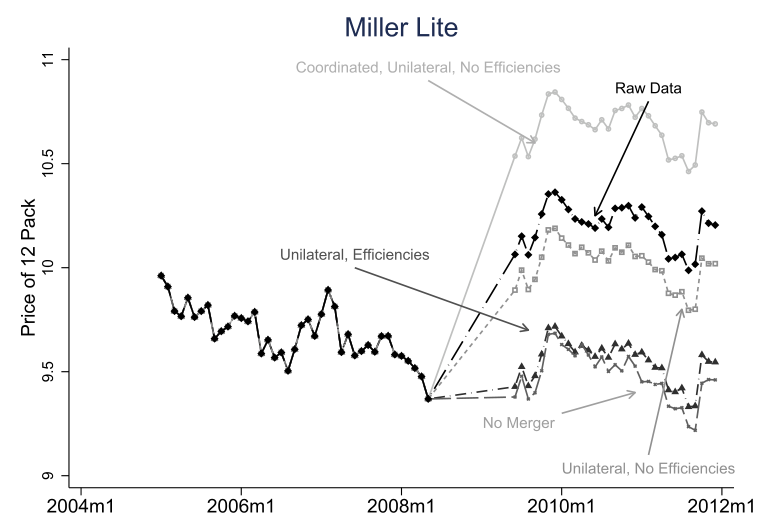
\includegraphics[width=0.82\textwidth]{figures/ch11/mw_fig4_counterfactual.png}
\caption{Counterfactual prices for Miller Lite 12 packs. The series before mid-2008 is the raw data. After the
excluded transition year, the figure shows the raw data and four counterfactual scenarios. They are no merger,
unilateral effects with efficiencies, unilateral effects without efficiencies, and coordinated and unilateral effects
without efficiencies. Each point is the average price across the 39 regions. Source: Miller and Weinberg (2017), Figure 4.}
\label{fig:11-mwcf}
\end{figure}

\begin{table}[htbp]
\centering
\caption{Results from the counterfactual analysis, 2011 (Miller and Weinberg 2017, Table X)}
\label{tab:11-mw-cf}
\footnotesize
\begin{tabular}{@{}lccccc@{}}
\toprule
Coordinated effects & yes & yes & no & no & no \\
Unilateral effects & yes & yes & yes & yes & no \\
Efficiencies & yes & no & yes & no & no \\
 & (i) & (ii) & (iii) & (iv) & (v) \\
\midrule
\multicolumn{6}{@{}l}{\textit{Retail prices (dollars)}} \\
ABI & 10.03 & 10.14 & 9.38 & 9.55 & 9.43 \\
Miller & 8.94 & 9.37 & 8.28 & 8.72 & 8.19 \\
Coors & 10.18 & 10.85 & 9.56 & 10.22 & 9.26 \\
\addlinespace
\multicolumn{6}{@{}l}{\textit{Brewer markups (dollars)}} \\
ABI & 4.45 & 4.56 & 3.81 & 3.97 & 3.84 \\
Miller & 4.52 & 4.32 & 3.83 & 3.63 & 3.05 \\
Coors & 4.25 & 4.06 & 3.61 & 3.41 & 2.68 \\
\addlinespace
\multicolumn{6}{@{}l}{\textit{Welfare statistics (percent change relative to column (v))}} \\
Producer surplus & 22.1 & 19.1 & 10.3 & 8.2 & base \\
\quad ABI & 10.3 & 19.8 & $-0.08$ & 9.3 & base \\
\quad Miller & 37.8 & 20.2 & 24.6 & 9.1 & base \\
\quad Coors & 47.8 & 12.9 & 34.7 & 3.5 & base \\
Consumer surplus & $-3.7$ & $-5.3$ & $-0.2$ & $-2.1$ & base \\
Total surplus & 1.3 & $-0.6$ & 1.8 & $-0.1$ & base \\
\bottomrule
\end{tabular}

\smallskip
\begin{minipage}{0.92\linewidth}
\footnotesize Notes: Prices and markups are volume-weighted means for the 12-pack flagship brands of ABI, Miller and
Coors. Welfare statistics are percent changes relative to the no-merger scenario (v), marked ``base'' (the paper prints a
dash), computed on all products.
Column (i) uses the raw data and the supply estimates, and columns (ii) to (v) are counterfactuals computed with
RCNL-1. All statistics are for 2011. Source: \citet[Table X, p.~1788]{MillerWeinberg2017}.
\end{minipage}
\end{table}

\begin{figure}[htbp]
\centering
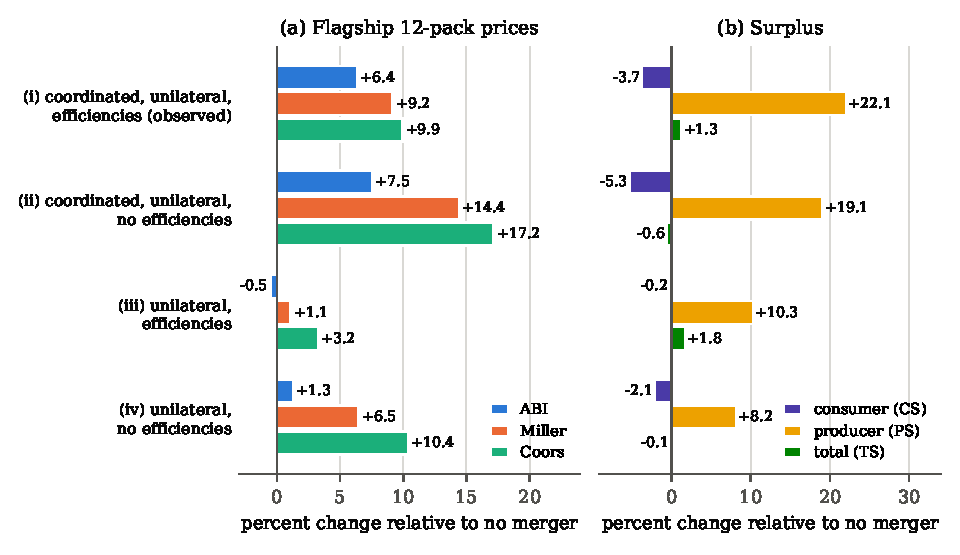
\includegraphics[width=\textwidth]{figures/ch11/mw_counterfactuals.pdf}
\caption{The counterfactual analysis of \cref{tab:11-mw-cf} relative to no merger. Panel (a) shows the percent change
in the volume-weighted price of each brewer's flagship 12 packs, computed from the table's prices. Panel (b) shows the
percent changes in consumer (CS), producer (PS) and total (TS) surplus reported in the table. Our computations from
Miller and Weinberg (2017), Table X.}
\label{fig:11-mwdecomp}
\end{figure}

Prices under no merger lie well below the raw data and roughly continue the pre-merger trend
(\cref{fig:11-mwcf}). The comparisons between columns isolate each channel. All differences below are our
calculations from \cref{tab:11-mw-cf}.

Unilateral effects are large. Moving from column (v) to column (iv) raises the Coors flagship price by \$0.96
(10.4 percent) and the Miller price by \$0.53 (6.5 percent). ABI's price rises by only \$0.12 (1.3 percent), through
strategic complementarity. Consumer surplus falls by 2.1 percent.

Efficiencies are also large, and they roughly offset the unilateral effects. Moving from column (iv) to column
(iii) lowers the Coors price by \$0.66 and the Miller price by \$0.44. ABI's price falls by \$0.17, to slightly below
its no-merger level. With unilateral effects and efficiencies, consumer surplus is only 0.2 percent below the
no-merger level and total surplus is 1.8 percent above it. This is the outcome the DOJ expected when it cleared the
joint venture. The prices of \cref{tab:11-mw-cf} also reveal the size of the efficiency. Price minus markup is ABI's
implied marginal cost, which stays at \$5.57 to \$5.59 in every column. Miller's implied cost is \$5.05 to \$5.14
without efficiencies and \$4.42 to \$4.45 with them. Comparing scenarios that differ only in efficiencies, (ii) with
(i) and (iv) with (iii), Miller's implied cost falls by \$0.63 and \$0.64. Both are close to $\hat\gamma_1 = -0.654$ in
RCNL-1.

Coordination adds a roughly uniform increment to the prices of all three brewers. Comparing column (i) with column (iii), and
column (ii) with column (iv), coordination raises the flagship price by \$0.59 to \$0.66 for each brewer, with and
without efficiencies. Relative to no merger, the observed prices are 6.4 percent higher for ABI, 9.2 percent for
Miller and 9.9 percent for Coors. Consumer surplus is 3.7 percent lower, so coordination accounts for about 3.5
percentage points of the consumer loss. Without efficiencies the loss would have been 5.3 percent.

Coordination is what makes the merger profitable for ABI. With unilateral effects and efficiencies alone, ABI's
producer surplus falls by 0.08 percent, because a more efficient MillerCoors takes sales from it. With coordination
it rises by 10.3 percent. The merging parties gain in every scenario, by 24.6 to 47.8 percent with efficiencies.

The welfare verdict depends on the standard. With coordination, total surplus is still 1.3 percent above the
no-merger level, so ``the antitrust clearance of the merger could be justified under a total welfare standard''
\citep[p.~1788]{MillerWeinberg2017}. Under a consumer surplus standard the merger harmed buyers. The four columns
also reveal the size of consumer surplus relative to total surplus. Solving $TS\% = w\,CS\% + (1-w)\,PS\%$ for the
weight $w$ gives 0.81 in every column, so consumer surplus is about 81 percent of total surplus in the no-merger
benchmark. A 1 percent loss to consumers therefore weighs about four times as much as a 1 percent gain to brewers.

\subsection{Robustness}\label{sec:11-mc-robust}

The paper's main robustness evidence is the spread across the five demand specifications. The estimate of $\kappa$
stays between 0.249 and 0.374 across nested logit and RCNL demand, monthly and quarterly data, and different sets of
income interactions (\cref{tab:11-mw-supply}). The cost coefficients are similarly stable. Four further checks bear on
the main threats.
\begin{enumerate}[label=(\alph*)]
\item A supplemental appendix adds a retail sector. Retail market power changes the
level of brewers' marginal costs but leaves brewer markups largely unaffected \citep[n.~14]{MillerWeinberg2017}.
\item An increasing marginal cost at ABI would bias $\hat\kappa$ upward. The paper
finds little evidence that ABI faced capacity constraints over the sample period \citep[n.~13]{MillerWeinberg2017}.
\item Two specifications ask whether the Great Recession, rather than the merger, triggered softer competition
\citep[Section~5.4]{MillerWeinberg2017}. With a separate $\kappa$ for each post-merger month, the estimates rise over
time as the economy recovers (their Figure~3). The second specification lets $\kappa$ vary with demeaned regional mean
income $\bar D_{rt}$ (unrelated to the aggregate diversion $\bar D$ of \cref{def:11-aggdiv}),
\begin{equation*}
  \kappa_{rt} = \frac{\exp(a_P\,\text{Post}_t + a_D\,\bar D_{rt})}{1 + \exp(a_P\,\text{Post}_t + a_D\,\bar D_{rt})} .
\end{equation*}
Here $a_P$ and $a_D$ are scalar parameters (the paper's $a$ and $b$). Under RCNL-3, $\hat a_P = 0.456$ (0.088) and
$\hat a_D = 0.033$ (0.039), which does not support countercyclical coordination. Under RCNL-1 the estimates are
noisier, $\hat a_P = 0.475$ (0.641) and $\hat a_D = -0.198$ (1.024) (pp.~1785--1786). The authors conclude: ``Given the totality of the evidence, we view the merger as the most likely
catalyst of softer price competition'' (p.~1786).
\item The paper's conclusion states that the price increases of MillerCoors and ABI,
``in both absolute terms and relative to their competitors,'' are ``visually evident and confirmed with econometric
analysis'' \citep[p.~1788]{MillerWeinberg2017}. The econometric analysis regresses the log real retail price on
post-merger indicators for MillerCoors products, for ABI products and for all products \citep[eq.~(1)]{MillerWeinberg2017}.
The regression includes product-by-region fixed effects and a linear time trend. The fullest specification adds
product-specific trends and regional employment and earnings and drops the year after the merger (Table II, column (iv)).
Its MillerCoors and ABI coefficients, which measure price changes relative to the imports, are 0.069 and 0.062, each
with a standard error of 0.007. The descriptive regressions also support the power of the supply instrument
(p.~1780).
\end{enumerate}

\subsection{Assessment}\label{sec:11-mc-assessment}

The paper's central finding is robust within its framework. Given the estimated demand system and the assumption of
parallel cost trends, ABI's post-merger prices are too high for Nash pricing. Whether the finding means that the
merger caused tacit coordination depends on several assumptions, which the literature and the paper itself discuss.

\casehead{What $\kappa$ measures}
By \cref{rem:11-mc-theta}, $\kappa$ is a conduct parameter, and the critique of \citet{Corts1999} applies. Suppose firms
play a repeated game in which the degree of cooperation varies over time. A single estimated weight then summarizes
average behavior, and it need not measure the true degree of collusion (\cref{ch:conduct}). The paper acknowledges the
point and notes that a nonzero $\kappa$ still rejects post-merger Nash pricing \citep[n.~12]{MillerWeinberg2017}. The
same footnote cites \citet{Bresnahan1989} and \citet{Porter1983} on identification with regime shifts. A related
concern is that $\kappa$ is not a structural primitive. Repeated-game theory (\cref{ch:collusion-theory}) predicts
that the sustainable degree of cooperation depends on costs, asymmetries and the number of firms. Scenario (ii)
removes the efficiencies but holds $\kappa$ at $\hat\kappa$. The efficiencies changed MillerCoors's costs and
margins, and with them the gains from cooperation and from deviation. The data do not reveal the value of $\kappa$
without efficiencies, so scenario (ii) is best read as a partial counterfactual.

\casehead{Price leadership}
The internalization weight summarizes outcomes. It leaves open the mechanism that produces them. Documents from the
DOJ's review pointed to leader-follower pricing, and the paper discusses qualitative evidence of price leadership that
surfaced in other beer litigation \citep[pp.~241--242]{AskerNocke2021}. In follow-on work, \citet{MillerSheuWeinberg2021}
investigate this price-leadership mechanism \citep[p.~242, n.~166]{AskerNocke2021}. In their model the leader, ABI, announces supermarkups over
Bertrand prices, and a coalition of ABI, Miller and Coors (later MillerCoors) adopts them
\citep[pp.~3124 and 3140]{MillerSheuWeinberg2021}. Their model gives a mechanism for the coordinated effects that the conduct parameter detects. It also connects this
case to the evidence on price leadership and tacit coordination in \cref{ch:collusion-evidence}.

\casehead{Confounds at the time of the merger}
The identifying assumption is parallel trends in unobserved marginal costs between ABI and the importers
(\cref{prop:11-mc-did}). Several events in the excluded window could violate it. InBev took control of Anheuser-Busch
in November 2008 \citep[p.~1784]{MillerWeinberg2017}, which could have changed ABI's costs or its pricing policy
independently of the joint venture. A change in ABI's objectives that raised its prices would load onto $\hat\kappa$.
The paper notes that the price increases of its Figure 1 predate the close of that deal (n.~16). Exchange rates moved
sharply in late 2008. The monthly average rate rose from 10.1 pesos per dollar in August 2008 to 13.4 in December
\citep{FederalReserve2026}. Corona is shipped from Mexico \citep[n.~4]{MillerWeinberg2017}, so import costs measured
in dollars need not have followed ABI's domestic costs. If import
costs fell relative to ABI's, the model reads ABI's relative price rise as a markup and $\hat\kappa$ is biased upward.
The recession is a further confound. The income interactions and the period effects absorb part of it, and the
domestic sales decline argues against pure down-market substitution. A recession that changed the relative demand for
domestic and imported beer in ways the income interactions miss would still bias the estimate.

\casehead{Retailers and the three-tier system}
The model treats brewers as setting retail prices. In practice brewers set prices to distributors, who set prices to
retailers. Hypothesis (H3), equal retail prices for the three flagship light beers, is a retail convention. The
structural model can only attribute such a pattern to brewer conduct. The retail appendix shows that brewer markups
are robust to retail market power, which addresses the level of costs but not retail pricing conventions.

\casehead{The Nash restriction on imports}
The supply model forces Modelo and Heineken to price as Nash players. The paper motivates this with qualitative
evidence \citep[pp.~1773 and 1779]{MillerWeinberg2017}. The DOJ's complaint against ABI's acquisition of Modelo
alleges that Modelo declined to match many of the price increases led by ABI.
Modelo instead followed a ``Momentum Plan'' designed to grow its share by shrinking its price gaps with domestic premium brands. The complaint does not address Heineken's pricing, and the
paper notes that Heineken's retail prices are similar to Corona's (p.~1773). Anheuser-Busch's equity stake in Modelo, mentioned in \cref{sec:11-mc-industry}, would by itself justify a positive
weight between ABI and Modelo in the sense of \citet{OBrienSalop2000}. Since the importers are the control group in
\cref{prop:11-mc-did}, any softening of their own conduct after the merger would change the comparison.

\casehead{Dependence on substitution patterns}
The estimate of $\kappa$ is the part of ABI's price rise that unilateral effects cannot explain, so it inherits every
restriction of the demand model. \Cref{tab:11-mw-elast} shows substitution close to proportional to shares, with no
special closeness among the domestic light beers. If Bud Light, Miller Lite and Coors Light were closer substitutes
than the RCNL implies, the Nash model would predict a larger response of ABI to MillerCoors's price increase. Less of
the rise would then be left for $\kappa$. A model with a light-beer or domestic nest, or with unobserved random
coefficients, would test this. The nested logit column is consistent with this direction. Its weaker
substitution among inside goods comes with the largest estimate, $\hat\kappa = 0.374$.

\casehead{Measuring efficiencies}
The MillerCoors post-merger indicator absorbs any change in MillerCoors's implied costs relative to the importers.
It therefore measures efficiencies as a residual, and anything else that lowered MillerCoors's implied costs would
be counted as an efficiency. Independent evidence comes from \citet{AshenfelterHoskenWeinberg2015}. They correlate
post-merger price changes across regions with the predicted change in concentration and the predicted reduction in
shipping distances. Larger increases in concentration went with larger price increases, and larger reductions in
shipping distance went with smaller ones \citep[p.~220]{AskerNocke2021}. The timing also differed. Market-power
effects arrived faster than the efficiencies, and cost reductions were ``not fully incorporated into pricing until
about two years after the merger's approval'' (p.~220). A residual measured soon after the merger may therefore
understate the long-run efficiency. The study gives direct evidence that the efficiencies were real. Whether they
were specific to the merger is less clear, as \cref{sec:11-agencies} discusses.

\casehead{Contribution}
\citet{MillerWeinberg2017} changed the empirical analysis of mergers in three ways. First, they showed how to test the
conduct assumption that every merger simulation maintains. They nested Nash pricing in a model with a post-merger
internalization weight and identified the weight from a consummated merger, with non-merging rivals as controls. Second, they
decomposed observed post-merger prices into unilateral effects, coordinated effects and efficiencies, and showed
that the decomposition reverses the welfare verdict between total and consumer surplus standards. Third, they provided
structural evidence for the agencies' concern that a merger can soften competition between the merged firm and its
rivals. The authors call this evidence ``somewhat novel in the empirical literature.'' That literature ``has focused
much more on understanding how mergers affect the unilateral pricing incentives of firms, holding the equilibrium
concept fixed'' \citep[p.~1788]{MillerWeinberg2017}. The case complements the validation exercise of \cref{sec:11-bv}. There a
unilateral-effects simulation underpredicted the observed price increase of the merging firms' rivals, and here a
structural model attributes a similar rival response to coordination.

\section{Beyond short-run prices: spatial markets, repositioning and investment}\label{sec:11-beyond}

The merger simulations of \cref{sec:11-simulation} hold three things fixed. They fix the set of products and
their characteristics. They fix each firm's capacity. They also summarize substitution with a demand system in
which location plays no explicit role. This section studies three papers that relax one of these restrictions
each. \citet{Houde2012} builds the geography of a retail market into demand and checks a merger simulation against
a difference-in-differences estimate of the same merger. \citet{Sweeting2010} documents how merging radio stations
change their programming, a dimension that a price-only analysis ignores. \citet{Pesendorfer2003} models capacity
investment and uses investment choices to infer the cost savings that mergers produced.

\subsection{Spatial competition and the Ultramar-Sunoco transaction: Houde (2012)}\label{sec:11-houde}

\casehead{Question}
How much does a merger of retail outlets raise prices when consumers are mobile? \citet{Houde2012} argues that the
relevant location of a gasoline buyer is the whole route she drives between home and work, not her home address.
Two stations far apart can then be close substitutes if many commuters pass both. Substitution depends on the road
network and on the direction of traffic. The paper asks two questions. Does a demand model built on commuting paths
fit the data better than the usual home-address model? Does a merger simulation based on it predict the price
effects of an observed merger, as measured by a retrospective difference-in-differences study?

The second question matters for the methodological debate of \cref{sec:11-retro,sec:11-bv}. A retrospective
estimate is transparent but tied to one sample and one control group. A simulation can evaluate any counterfactual
but rests on a demand model. Comparing the two on the same merger is a validation exercise in the spirit of
\citet{LaLonde1986}, who compared nonexperimental estimators with an experimental benchmark. Here the demand model is
estimated without the supply restrictions that the merger imposes, so the comparison is a true out-of-sample test.

\casehead{Setting}
The market is the Quebec City census metropolitan area between 1991 and 2001. Five major brands were present:
Shell, Esso, Petro-Canada, Irving and Ultramar. Ultramar was the leading chain and the only firm with a refinery
near the city. The 1990s brought a large reorganization of North American gasoline retailing. Technology raised the
efficient size of stations, the value of small repair garages fell, and new environmental rules forced owners to
replace underground storage tanks. The number of stations in Quebec City fell by 30 percent, from 382 in 1991 to
283 in December 2001, mostly through exit by stations of the major chains \citep[p.~2152]{Houde2012}.

Two further facts shape the analysis. Prices are tightly clustered. Over most of the period the interquartile range
of prices was below one cent per litre (cpl), about 1.5 percent of the average price. Retail margins over the rack
price, the wholesale price posted at the terminal, ranged between 8 and 15 percent of the price for most of the
period. There were also two price wars. The first, in the summer of 1996, followed excess capacity and a low-price
guarantee campaign by Ultramar. In 2000 average margins fell to zero after several stations priced at a regulated
price floor, introduced by a provincial law of December 1996 \citep[pp.~2152--2153]{Houde2012}.

\casehead{Data}
The station data come from Kent Marketing, a survey firm that visits every station at the end of each survey period
and reads the volume sold off the pump meters. The panel has 46 bimonthly periods between 1991 and 2001, with only the
fourth period observed in the first four years. It contains 14,263 station-period observations on 429 station sites.
Observed characteristics include the size of the convenience store, a repair-shop indicator, the numbers of
service islands and pumps, opening hours, brand, type of service and a car wash. The price is the posted unleaded
price on the survey day, deflated by the regional consumer price index. Average volume was 4,934 litres per day
(standard deviation 3,289), and the average real price was 63.83 cpl (Table~1). About 8 percent of the sample
stations refused the survey in some or all periods. Their characteristics and prices are observed, and Houde imputes
their volumes by linear regression on neighborhood shares, predicted traffic, population density, location, prices,
characteristics and lagged sales \citep[p.~2151, n.~12]{Houde2012}.

Table~1 also shows how much the stations changed over the decade. From fall 1991 to fall 2001 average volume rose from
3,949 to 6,271 litres per day, and the number of pumps from 7.77 to 11.37. The share of full-service stations fell
from 0.54 to 0.28. The average absolute deviation of a station's price from the period mean fell from 0.90 to 0.13 cpl,
as most stations came to post the modal price \citep[p.~2152]{Houde2012}.

The geography comes from three sources. A road network with more than 30,000 street segments gives travel times,
and a shortest-path algorithm gives each commuter's route. Origin-destination surveys from 1991, 1996 and 2001 give
the number of commuters between traffic zones, by purpose and mode. Census and labor-force data give the population
and the income distribution of each residential area. Commuters who cross the city on highways are proxied by
occupied hotel rooms. Before estimating any model, \citet[Figure 2]{Houde2012} compares station sales with two
crude predictions. If consumers buy at random from stations within half a minute of their commuting path, predicted
and observed shares have a correlation near 0.3 in every period. If they buy at random near home, the correlation is
near zero or negative.

\casehead{Model}
Consumer $i$ commutes from home location $s_i$ to work location $d_i$ along the fastest route $r(s_i, d_i)$. The
route takes time $t(s_i,d_i)$ and covers $m(s_i,d_i)$ kilometers. Station $j$ sits at location $l_j$. The consumer
buys from one of the $J$ stations or takes the outside option $j = 0$, which is to commute without a car. Her
indirect utility is \citep[eq.~(1)]{Houde2012}
\begin{equation}\label{eq:11-houde-u}
u_{ij} =
\begin{cases}
x_j\beta + (\bar\alpha + \alpha_y y_i)\,p_j + \lambda_1\,\mathcal{D}\big(r(s_i,d_i), l_j\big) + \xi_j + \epsilon_{ij},
& j = 1,\dots,J,\\[2pt]
-\lambda_0\,\mathit{Long}(s_i,d_i) + \epsilon_{i0}, & j = 0.
\end{cases}
\end{equation}
Here $x_j$ collects station characteristics, brand and period dummies, $\xi_j$ is unobserved station quality,
$y_i$ is the log hourly wage, and $\epsilon_{ij}$ is type-I extreme value. The indicator $\mathit{Long}(s,d)$
equals one when home and work lie in different traffic zones. Houde writes $C(s,d)$ for it, and we rename it to avoid
confusion with cost functions. Long commuters are more likely to drive, so we expect
$\lambda_0 > 0$. The paper writes the price term as $+(\bar\alpha + \alpha_y y_i)\,p_j$ (eq.~(1) and p.~2157), and
the estimated $\bar\alpha$ is negative (Table~3). In the sign convention of this book the consumer's price
coefficient is therefore $\alpha_i = -(\bar\alpha + \alpha_y y_i)$. The symbols $\lambda_0$ and $\lambda_1$ are local
to this subsection.

The novel object is the \emph{detour} $\mathcal{D}$. It measures the extra driving time needed to stop at $l$ on the
way from $s$ to $d$:
\begin{equation}\label{eq:11-houde-detour}
\mathcal{D}\big(r(s,d), l\big) = t(s,l) + t(l,d) - t(s,d).
\end{equation}
A station on the route costs no extra time. The standard single-address model is nested as the special case in which
the consumer starts and ends at home, $\mathcal{D}^h(s,l) = 2\,t(s,l)$. Transport costs make utility fall with the
detour, so we expect $\lambda_1 < 0$. \Cref{fig:11-detour} illustrates the difference between the two metrics.

\begin{figure}[htbp]
\centering
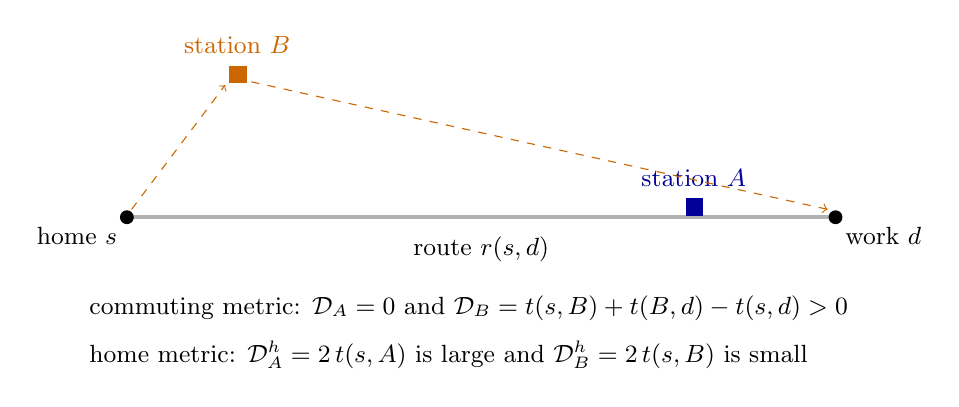
\begin{tikzpicture}[every node/.style={font=\small}]
  \draw[line width=1.6pt, gray!60] (0,0) -- (9,0);
  \node[below] at (4.5,-0.12) {route $r(s,d)$};
  \fill (0,0) circle (2.5pt) node[below left] {home $s$};
  \fill (9,0) circle (2.5pt) node[below right] {work $d$};
  \fill[blue!60!black] (7.1,0.02) rectangle +(0.22,0.22);
  \node[above, blue!60!black] at (7.2,0.27) {station $A$};
  \fill[orange!80!black] (1.3,1.7) rectangle +(0.22,0.22);
  \node[above, orange!80!black] at (1.4,1.95) {station $B$};
  \draw[dashed, orange!80!black, ->] (0.06,0.1) -- (1.25,1.68);
  \draw[dashed, orange!80!black, ->] (1.58,1.72) -- (8.9,0.1);
  \node[anchor=west] at (-0.6,-1.15) {commuting metric: $\mathcal{D}_A = 0$ and $\mathcal{D}_B = t(s,B) + t(B,d) - t(s,d) > 0$};
  \node[anchor=west] at (-0.6,-1.75) {home metric: $\mathcal{D}^h_A = 2\,t(s,A)$ is large and $\mathcal{D}^h_B = 2\,t(s,B)$ is small};
\end{tikzpicture}
\caption{Two distance metrics in the demand model of \citet{Houde2012}. Station $A$ lies on the commuter's route
near her workplace, so it requires no detour although it is far from home. Station $B$ is close to home but off the
route. The commuting metric ranks $A$ closer, and the home metric ranks $B$ closer.}
\label{fig:11-detour}
\end{figure}

Gasoline demand is inelastic at the individual level. A consumer of type $(s,d)$ who buys at all buys
$\bar q(s,d) = \bar q_0 + \bar q_1 m(s,d)$ litres, where $\bar q_1$ is fixed at the average fuel use of a city car and
$\bar q_0$ is estimated. Houde writes $c_0$ and $c_1$ for these parameters. The text fixes $\bar q_1$ at 0.10 litres
per kilometer (p.~2156), while Tables~3 and 4 list the fixed value as 0.2. The paper does not reconcile the two
numbers. With $T_{s,d}$ commuters between $s$ and
$d$, market size is $M = \sum_s\sum_d \bar q(s,d)\,T_{s,d}$ (eq.~(2)). Write the inside utility net of the
logit shock as $V_{ij} = \delta_j + (\bar\alpha + \alpha_y y_i)p_j + \lambda_0\mathit{Long}(s_i,d_i) +
\lambda_1\mathcal{D}(r(s_i,d_i),l_j)$, where $\delta_j = x_j\beta + \xi_j$. Adding $\lambda_0\mathit{Long}$ to every
inside option normalizes the outside utility to zero. The choice probability and station demand are (eqs.~(3)--(4))
\begin{equation}\label{eq:11-houde-demand}
P_{ij} = \frac{\exp(V_{ij})}{1 + \sum_{k=1}^{J}\exp(V_{ik})},
\qquad
Q_j(p) = \sum_s\sum_d \bar q(s,d)\, T_{s,d}\int P_{j}\big(r(s,d), y\big)\, dF(y \mid s),
\end{equation}
where $F(y \mid s)$ is the wage distribution in home area $s$. The integral is computed by simulation.

Houde also estimates a discrete-continuous alternative, in which each consumer's quantity responds to price through
Roy's identity. The demand results are unchanged. The supply results, however, imply that firms behave as strategic
substitutes after a simulated merger, so that competitors cut their prices. Houde attributes this to conditional
demand that is inelastic for most consumers and treats the functional form as inaccurate \citep[p.~2157,
n.~24]{Houde2012}.

The commuting structure determines substitution through the following algebra. Write $a_i = \bar\alpha + \alpha_y
y_i < 0$ and let $\sum_i h_i(\cdot)$ denote the sum over consumer types, with weights $h_i = \bar q(s_i,d_i)
T_{s_i,d_i}\,\dd F(y_i \mid s_i)$. The logit derivatives are $\frac{\partial P_{ij}}{\partial p_j} = a_i P_{ij}(1 -
P_{ij})$ and $\frac{\partial P_{ik}}{\partial p_j} = -a_i P_{ij}P_{ik}$. Summing over types gives the diversion
ratio from $j$ to $k$ of \cref{def:04-diversion}:
\begin{align}
D_{jk}
= -\dfrac{\frac{\partial Q_k}{\partial p_j}}{\frac{\partial Q_j}{\partial p_j}}
&=\frac{\sum_i h_i (-a_i) P_{ij} P_{ik}}{\sum_i h_i (-a_i) P_{ij}(1 - P_{ij})} \notag\\
&= \sum_i \underbrace{\frac{h_i (-a_i) P_{ij}(1 - P_{ij})}{\sum_{i'} h_{i'} (-a_{i'}) P_{i'j}(1 -
P_{i'j})}}_{\text{weight of type } i}\; \frac{P_{ik}}{1 - P_{ij}} . \label{eq:11-houde-diversion}
\end{align}
For each type the diversion is the logit ratio $\frac{P_{ik}}{1 - P_{ij}}$ of \cref{ch:logit}, proportional to $k$'s
share. Aggregate diversion averages these ratios with weights that are large for the types who buy at $j$ and are
price sensitive. Station $k$ therefore captures much of $j$'s lost volume when the commuters who patronize $j$ also
pass close to $k$. This is how the road network enters the substitution matrix, and why stations far apart can be
close substitutes. A home-address model weights types by where they live and misses this channel.

\casehead{Estimation}
The parameters $(\bar q_0, \lambda_0, \lambda_1, \alpha_y, \bar\alpha, \beta)$ are estimated by the nested fixed point
GMM method of \citet{Berry1994} and \citet{BerryLevinsohnPakes1995} (\cref{ch:blp}). Two sets of moments are combined.
The first follows \citet{Nevo2001} and uses station-location fixed effects. Write $\xi_{jt} = \bar\xi_j +
\tilde\xi_{jt}$, where $\bar\xi_j$ is the permanent quality of the site (ease of access, side of the street) and
$\tilde\xi_{jt}$ a transitory shock. With $\tilde w_{jt}$ the within-station deviation of a variable, the moments are
(eq.~(5))
\begin{equation}\label{eq:11-houde-m1}
\bar g^1_n(\theta) = \frac{1}{n}\sum_{j,t}\tilde\xi_{jt}(\theta)\,\tilde W^1_{jt},
\end{equation}
where $\tilde W^1_{jt}$ contains the within-transformed station characteristics, the excluded instruments $z_{jt}$
and period dummies.

The second set is a micro moment that disciplines the outside option. The 2001 origin-destination survey reports
the share of commuters between each pair of zones who drive. The model predicts the same share as one minus the
probability of the outside option, $U_{sd}(\theta)$. With $\hat U_{sd}$ the observed share, the moments are
(eq.~(6))
\begin{equation}\label{eq:11-houde-m2}
\bar g^2_{n_2}(\theta) = \frac{1}{n_2}\sum_{s,d}\big(U_{sd}(\theta) - \hat U_{sd}\big)W^2_{sd},
\end{equation}
with $W^2_{sd}$ a constant, the long-commute indicator and simulated income. These moments force the model to
reproduce a reduced-form regression estimated on 3,000 simulated survey respondents (eq.~(7)):
\begin{equation}\label{eq:11-houde-carreg}
\hat U_i = \underset{(0.033)}{0.247} + \underset{(0.0141)}{0.0495}\; y_i + \underset{(0.0163)}{0.315}\;
\mathit{Long}_i, \qquad R^2 = 0.47 .
\end{equation}
The intercept pins down $\bar q_0$ and hence market size, the income slope pins down $\alpha_y$, and the
long-commute slope pins down $\lambda_0$. The weighting matrix allows for serial and spatial correlation in
$\tilde\xi_{jt}$. With 46 periods and more than 300 stations, the inner loop is costly. Houde inverts demand with a
derivative-free quasi-Newton algorithm, which is faster than the contraction mapping of
\citet{BerryLevinsohnPakes1995}. The inner-loop tolerance is $10^{-12}$, tightened to $10^{-14}$ for the standard
errors \citep[p.~2160, n.~27]{Houde2012}.

\casehead{Instruments and identification}
Two parameters need excluded variation: the price coefficient $\bar\alpha$ and the transport cost $\lambda_1$. Prices
are endogenous because firms see $\xi_{jt}$ and because frequent price changes make the survey-day price a noisy
measure of the price that generated the period's volume. The transport cost enters nonlinearly, and it is identified
by how a station's sales respond to changes in its neighbors.

The identifying assumption is that the transitory quality shock $\tilde\xi_{jt}$ evolves independently of the
characteristics of nearby stations, conditional on location fixed effects. The industry reorganization supplies the
variation. Stations closed, opened and were rebuilt for reasons of technology and regulation that were unrelated to
local demand shocks. Entry, exit and remodeling involve large sunk costs, so they plausibly respond to $\bar\xi_j$
but not to $\tilde\xi_{jt}$. Cross-sectional versions of this argument, which assume that location quality is
independent of neighbors' characteristics, would bias the transport cost toward zero if stations locate at
high-traffic, high-quality sites \citep[p.~2160]{Houde2012}.

Competitors' characteristics are weak instruments for price, because cross-sectional price dispersion is small. Rack
prices vary mostly over time and are absorbed by period effects. Houde therefore exploits small differences in the
posted rack prices of two suppliers. Sunoco supplied the Quebec City terminal until 1997, and the independent
wholesaler Olco took over afterward. The instruments interact the Sunoco and Olco rack prices with indicators for a
Sunoco or Olco station in the neighborhood of station $j$. Table~2 of the paper defines four instrument sets.
Specification (1) uses the count and average size of competitors on the same street and the average competitor size
within 0.1, 0.33 and 1 kilometer (5 instruments). Specification (2) uses the rack-price interactions (4
instruments). Specification (3) combines the two, and specification (4) adds the fractions of competitors with
various amenities (25 instruments in that set). Two stations share a street if they have a street in common and
are within five minutes of each other. The first-stage F-statistics exceed 10 for specifications (2) and (3).

\casehead{Demand results}
\Cref{tab:11-houde-demand} reproduces the estimates of the multi-address (commuting) model and of the single-address
(home) model. The two models differ most in the transport cost. In the commuting model $\lambda_1$ is negative, large
and precise, except in specification (2), which uses only the cost instruments. In the home model it is positive in
every specification, so consumers would prefer stations farther from home. The correlations in Figure~2 of the paper
explain the sign. Large stations sit at the intersections of major commuting routes, often far from where people live,
so the home model can rationalize their sales only with a small or positive transport cost.

\begin{table}[htbp]
\centering
\caption{Demand estimates for Quebec City gasoline stations}
\label{tab:11-houde-demand}
\begin{threeparttable}
\small
\begin{tabular}{@{}lcccc@{}}
\toprule
 & (1) & (2) & (3) & (4) \\
\midrule
\multicolumn{5}{@{}l}{\emph{Panel A. Multi-address (commuting) model, Table 3}} \\
Minimum consumption $\bar q_0$ & 4.5746 & 4.5290 & 4.5582 & 4.5035 \\
 & (0.0334) & (0.0442) & (0.0299) & (0.0242) \\
Income $\alpha_y$ & 0.0396 & 0.1082 & 0.0474 & 0.1677 \\
 & (0.0307) & (0.0809) & (0.0327) & (0.0482) \\
Long commuters $\lambda_0$ & 1.4972 & 1.4356 & 1.4768 & 1.3891 \\
 & (0.0326) & (0.0683) & (0.0299) & (0.0432) \\
Transportation cost $\lambda_1$ & $-1.2777$ & $-0.5642$ & $-1.0004$ & $-0.3961$ \\
 & (0.537) & (0.29) & (0.291) & (0.0909) \\
Price $\bar\alpha$ & $-0.2181$ & $-0.1687$ & $-0.1974$ & $-0.1490$ \\
 & (0.0767) & (0.033) & (0.0378) & (0.0233) \\
Median travel cost (cpl per minute) & 5.886 & 3.398 & 5.098 & 2.733 \\
$J$-statistic (degrees of freedom) & 3.07 (3) & 1.22 (2) & 6.06 (7) & 40.5 (27) \\
\addlinespace
\multicolumn{5}{@{}l}{\emph{Panel B. Single-address (home) model, Table 4}} \\
Minimum consumption $\bar q_0$ & 5.0992 & 5.0399 & 5.1246 & 4.9940 \\
 & (0.158) & (0.0965) & (0.0691) & (0.0706) \\
Income $\alpha_y$ & $-0.8433$ & $-0.6463$ & $-0.9318$ & $-0.4574$ \\
 & (0.87) & (0.409) & (0.36) & (0.226) \\
Long commuters $\lambda_0$ & 3.6236 & 2.9233 & 3.9919 & 2.4657 \\
 & (2.53) & (1.07) & (1.06) & (0.534) \\
Transportation cost $\lambda_1$ & 0.5556 & 0.4235 & 0.6152 & 0.3181 \\
 & (0.519) & (0.235) & (0.211) & (0.126) \\
Price $\bar\alpha$ & $-0.1498$ & $-0.0918$ & $-0.1054$ & $-0.0630$ \\
 & (0.0543) & (0.0252) & (0.0275) & (0.0176) \\
Median travel cost (cpl per minute) & $-3.258$ & $-3.933$ & $-4.793$ & $-4.284$ \\
$J$-statistic (degrees of freedom) & 10.2 (3) & 3.83 (2) & 14.2 (7) & 60.6 (27) \\
\addlinespace
5 percent $\chi^2$ threshold & 7.82 & 5.99 & 14.1 & 40.1 \\
\bottomrule
\end{tabular}
\begin{tablenotes}[flushleft]
\footnotesize
\item Notes: Reproduced from \citet[Tables 3 and 4]{Houde2012}, with the paper's signs (a negative $\bar\alpha$ means
that utility falls with price, a negative $\lambda_1$ that it falls with the detour). Standard errors robust to serial
and spatial correlation in parentheses. The commuting-distance coefficient $\bar q_1$ is fixed. Both tables list it as
0.2, although the text fixes it at 0.10 litres per kilometer (p.~2156). The income row is the coefficient on the log hourly wage, scaled as in the paper. Columns use the instrument sets (1) to (4)
described in the text. All specifications include location, time and brand fixed effects and time-varying station
characteristics. The travel cost is the ratio of $\lambda_1$ to the price coefficient at the median wage. There are
14,263 observations on 429 stations in every column.
\end{tablenotes}
\end{threeparttable}
\end{table}

The price coefficient implies station-level own-price elasticities between $-10$ and $-15$, which fits a market of
nearly homogeneous products. The ratio of $\lambda_1$ to the price coefficient prices a minute of detour. Its median
is about 5 cpl per minute in specification (3). For a 20-litre purchase, Houde converts this into about \$0.9 per
minute of shopping, or \$54 per hour, four times the average hourly wage \citep[p.~2163]{Houde2012}. He reads the
number as an upper bound on the value of time, because the detour measure ignores congestion and the cost of
re-planning a route. A large transport cost does not mean that consumers face few options. The average consumer
passes 10 stations within one minute of her route, and long commuters pass more.

The $J$-statistics favor the commuting model. Its statistics are below the 5 percent $\chi^2$ thresholds in
specifications (1) to (3) and slightly above it in (4). The single-address model's statistics are roughly twice as
large and exceed the thresholds in all specifications except (2). Specification (3) of the commuting model is
the preferred specification and the basis of the merger analysis.

Tables 5 and 6 of the paper describe the implied substitution matrix on a 10 percent random sample of station pairs.
Cross-price elasticities are very skewed. Their mean is 0.025 and their median 0.0013, while the 99th percentile is
0.397 and the maximum 5.26. Each station has two or three close competitors, located within about 1.25 minutes and
sharing more than 70 percent of traffic. Table~6, column 3, regresses normalized cross elasticities on pair
characteristics. The coefficient on the share of common traffic is 0.449 (0.0178), on driving time $-0.00105$
(0.0000716), and on sharing a street 0.0611 (0.00812), with $R^2 = 0.453$. Commuting patterns and driving times alone
explain about half of the variation in substitution.

\casehead{The transaction}
In March 1996 Ultramar and Sunoco announced a swap of retail networks. Ultramar acquired 127 Sunoco stations in
Quebec, and Sunoco acquired 88 Ultramar sites in Ontario. Sunoco had no refinery in Quebec, while Ultramar wanted to
sell more of its Saint-Romuald refinery's output locally. The Competition Bureau had studied the proposal in December
1995 and deemed it unlikely to lessen competition substantially. Sunoco stopped supplying its Quebec City terminal on
January 1, 1997, and Olco began selling unbranded gasoline from it. The first Sunoco station was rebranded in the
second quarter of 1997, and the paper dates the merger to January 1997 \citep[p.~2167]{Houde2012}.

The transaction is \emph{vertical} in form and horizontal in effect. From January 1997 Ultramar supplied the former
Sunoco stations, and through its contracts it controlled their retail prices. In Quebec City, Sunoco had 12 stations
in December 1996. Ultramar went from 50 to 62 stores and from 16 to 20 percent of the market. Table~7 of the paper
tracks the rebranding. Sunoco-branded stations numbered 12 in January 1997 and 6, 3 and 0 in January 1998, 1999 and
2000. Over the same dates, 0, 5, 8 and 10 stations carried the Ultramar brand after rebranding. Of the 313 stations
active in January 1997, 5.3 percent lay within half a minute of a Sunoco station, 6.3 percent within one minute and
10.1 percent within 1.5 minutes. The common-street neighborhood, made of stations that share a street with a Sunoco
station, contained 31.4 percent. These neighborhoods overlap, so the fractions do not add up.

\casehead{Supply and marginal costs}
Majors sell through company-owned stations, commission agents and lessee dealers. In the first two the supplier sets
the retail price. In 2001 between 52 and 72 percent of branded stations were company-owned \citep[p.~2168]{Houde2012}. Ultramar used commission contracts throughout and so acted as a vertically integrated chain. The
other majors set station-specific wholesale prices weekly and gave lessees a price-support clause that guaranteed a
minimum margin. Houde therefore assumes \emph{resale price maintenance} (RPM): each brand supplier $f$ chooses the
retail prices of all its stations $\mathcal{J}_f$ (eq.~(8)),
\begin{equation*}
\max_{\{p_j\}_{j \in \mathcal{J}_f}} \sum_{j \in \mathcal{J}_f}(p_j - c_j)\,Q_j(p_f, p_{-f}).
\end{equation*}
Let $\Delta^Q$ be the Jacobian of station volumes, with $(j,k)$ element $\frac{\partial Q_j}{\partial p_k}$, and let
$\Omega$ be the brand ownership matrix. In the stacked form of \cref{sec:11-simulation}, the first-order conditions and
the implied marginal costs are
\begin{equation}\label{eq:11-houde-foc}
Q(p) + \big(\Omega \odot \Delta^Q\big)^{\top}(p - c) = 0
\quad\Longrightarrow\quad
c = p + \big[(\Omega \odot \Delta^Q)^{\top}\big]^{-1} Q(p).
\end{equation}
Houde writes the same condition as $Q + (\Omega * \Delta)(p - c) = 0$ with $\Delta_{ij} = \frac{\partial Q_j}{\partial
p_i}$, which is our transposed Jacobian (eqs.~(9)--(10)).

Table~8 of the paper compares sales-weighted Lerner indices $\frac{p - c}{p}$ under four conduct assumptions. With
the commuting model they are 0.0970 when every station prices independently, 0.101 when station owners price jointly,
0.1036 under RPM and 0.2684 under joint profit maximization. The observed margin over the average rack price, net of
consumption taxes, is 0.0898. The RPM markups are close to this benchmark and imply a station marginal cost about one
percentage point below the rack price. The home model gives 0.1414, 0.1504, 0.1576 and 0.858 under the same four
assumptions, so its RPM markups are about 50 percent higher than those of the commuting model. The comparison
excludes 2000, 2001 and the summer of 1996.

Houde then decomposes marginal cost into a supplier-period wholesale component and station characteristics,
\begin{equation}\label{eq:11-houde-cost}
c_{jt} = Z_{jt}\zeta + w_{f(j),t} + \eta_{jt}.
\end{equation}
The equation is estimated by OLS with supplier-by-period fixed effects on the sample before 2000, excluding the 1996
price war (eqs.~(10)--(11)). Each regular pump lowers marginal cost by 0.0231 cpl (0.0061), and full service raises it by 0.171
(0.08). A car wash lowers it by 0.152 (0.062), and a repair shop raises it by 0.236 (0.082). The coefficient on the absence of a
convenience store is printed as 117 (0.062). Given the standard error and the text, which says that stations with a
convenience store have lower costs, it must be 0.117.
Lessee dealers are not significantly different from company-owned stations, 0.088 (0.072), and $R^2 = 0.92$. The
fixed effects $\hat w_{f,t}$ track the posted rack price closely after 1993 (Figure~3 of the paper). Independents
face wholesale costs a little more than one cent above Ultramar's. The decomposition lets the simulation give former
Sunoco stations Ultramar's upstream cost, which measures the efficiency side of the transaction.

\casehead{Merger simulation}
The simulation uses only pre-merger data. For each survey period, Houde solves the RPM
equilibrium with the former Sunoco stations added to Ultramar's ownership set, holding marginal costs fixed. He then
measures the simulated price change in four treatment neighborhoods around Sunoco stations: within half a minute,
one minute, 1.5 minutes, and on a common street. The control group is all other stations. The difference between the
average changes in the two groups is the simulated analogue of a difference-in-differences coefficient. The paper
describes the simulated periods in two ways. The text covers every period from 1995 to 1997 except June and July 1996
(p.~2171). The notes to Tables 9 and 10 cover January to December 1996, excluding June. Both versions leave out the
price war of summer 1996, and the numbers below are those of the tables.

Table~9 of the paper reports average simulated price changes of 0.406, 0.343, 0.219 and 0.101 cpl in the four
treatment groups. The matching control groups change by 0.019, 0.019, 0.019 and 0.011 cpl. The simulated
difference-in-differences effects are therefore 0.388, 0.325, 0.200 and 0.090 cpl, decreasing quickly with distance.
\Cref{tab:11-houde-sim} decomposes the half-minute effect. The \emph{direct effect} is the price change at stations
supplied by Ultramar after the merger, which internalize the diversion between Ultramar and former Sunoco outlets.
The \emph{indirect effect} is the response of competitors to those price increases.

\begin{table}[htbp]
\centering
\caption{Simulated effects of the Ultramar-Sunoco merger on prices (cpl), half-minute neighborhood}
\label{tab:11-houde-sim}
\begin{threeparttable}
\small
\begin{tabular}{@{}llccccc@{}}
\toprule
 & & \multicolumn{2}{c}{Chain (RPM)} & Owner & \multicolumn{2}{c}{Restricted choice set} \\
\cmidrule(lr){3-4}\cmidrule(lr){6-7}
 & & Status quo & Cost adjusted & Status quo & Chain & Owner \\
\midrule
Sunoco price changes & & 0.526 & 0.486 & 0.607 & 0.452 & 0.516 \\
 & & (0.173) & (0.351) & (0.202) & (0.219) & (0.234) \\
\addlinespace
Direct effect & In & 0.460 & 0.429 & 0.523 & 0.409 & 0.459 \\
 & & (0.200) & (0.331) & (0.243) & (0.212) & (0.237) \\
 & Out & 0.102 & 0.103 & 0.101 & 0.087 & 0.086 \\
 & & (0.105) & (0.107) & (0.104) & (0.132) & (0.131) \\
 & Difference & 0.357 & 0.326 & 0.422 & 0.323 & 0.373 \\
\addlinespace
Indirect effect & In & 0.026 & 0.025 & 0.026 & 0.064 & 0.066 \\
 & & (0.105) & (0.107) & (0.104) & (0.132) & (0.131) \\
 & Out & 0.002 & 0.002 & 0.000 & 0.002 & 0.001 \\
 & & (0.003) & (0.003) & (0.009) & (0.004) & (0.008) \\
 & Difference & 0.023 & 0.022 & 0.025 & 0.062 & 0.066 \\
\bottomrule
\end{tabular}
\begin{tablenotes}[flushleft]
\footnotesize
\item Notes: Reproduced from \citet[Table 10]{Houde2012}. Average simulated price changes between January and
December 1996, in cents per litre. Numbers in parentheses are standard deviations of the simulated changes across
stations, which measure heterogeneity, not sampling error. ``In'' and ``Out'' refer to stations within and beyond half
a minute of a Sunoco station. Direct effects are computed at Ultramar, Sunoco and Sergaz stations, and indirect effects
at all other stations. Chain: resale price maintenance by brand suppliers. Owner: station owners set prices. Cost
adjusted: former Sunoco stations get Ultramar's upstream cost. Restricted choice set: consumers choose among the 10
stations closest to their route.
\end{tablenotes}
\end{threeparttable}
\end{table}

Four features of the simulation stand out. Former Sunoco stations raise prices by 0.526 cpl on average, with a range
from about 0.2 to nearly 1 cpl across stations. Giving them Ultramar's lower upstream cost reduces this by only about
0.05 cpl, because Sunoco was estimated to be almost as efficient. Ultramar stations outside the half-minute
neighborhood raise prices by 0.102 cpl, so a retrospective study that used them as controls would understate the
direct effect (0.460 against a difference of 0.357). This is the control-group bias of \cref{prop:11-didbias}. Finally,
competitors respond very little, raising prices by 0.026 cpl. Houde attributes this to the logit shock, which spreads
substitution over all stations and the outside good. When consumers can choose only among the 10 stations nearest to
their route, the competitors' response more than doubles, to 0.064 cpl, while the direct effect barely changes.

\begin{figure}[htbp]
\centering
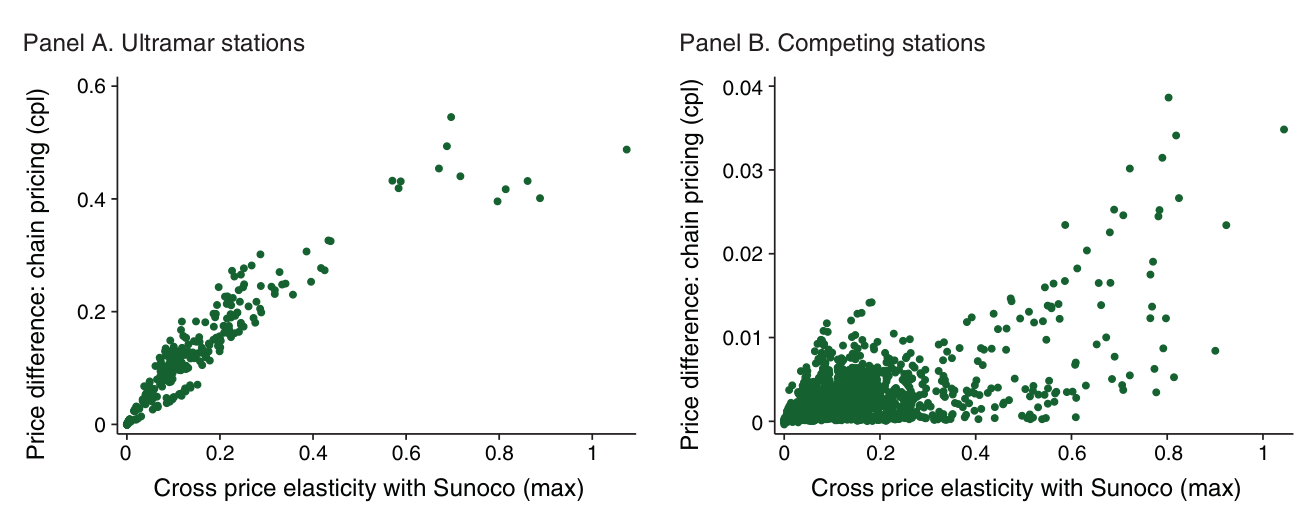
\includegraphics[width=0.92\textwidth]{figures/ch11/houde_fig4.png}
\caption{Simulated post-merger price changes (chain pricing, cpl) at Ultramar stations (panel A) and at competing
stations (panel B), plotted against each station's maximum cross-price elasticity with a Sunoco station. Note the
different vertical scales. Source: \citet{Houde2012}, Figure 4.}
\label{fig:11-houde}
\end{figure}

\Cref{fig:11-houde} shows where the price effects come from. Ultramar stations that compete closely with a Sunoco
station raise prices most, and the relation with the maximum cross elasticity is almost linear. The competitors'
responses follow the same pattern on a scale about fifteen times smaller and with more noise. Single-station owners
react more strongly to a close competitor's price increase than multi-station chains do.

\casehead{Retrospective analysis}
The difference-in-differences design follows \citet{Hastings2004}. Let $N^d_j$ indicate that station $j$ lies in
neighborhood $d$ of a Sunoco station, and let $T_t$ indicate periods from 1997 on. The indicator $S_{jt}$ marks stations
supplied by Ultramar after the merger (Ultramar, former Sunoco and Sergaz stations). The two regressions are (eqs.~(12)--(13))
\begin{align}
p_{jt} &= \gamma\, N^d_j T_t + Z_{jt}\omega + \mu_j + \tau_t + u_{jt}, \label{eq:11-houde-did}\\
p_{jt} &= \gamma_0\, N^d_j T_t S_{jt} + \gamma_1\, N^d_j T_t (1 - S_{jt}) + Z_{jt}\omega + \mu_j + \tau_t + u_{jt},
\label{eq:11-houde-did2}
\end{align}
with station fixed effects $\mu_j$, period effects $\tau_t$ and time-varying characteristics and sales volume in
$Z_{jt}$. The coefficient $\gamma$ is the average merger effect in the neighborhood, $\gamma_0$ the direct effect and
$\gamma_1$ the competitive effect. Identification requires that, absent the merger, prices in treated and control
neighborhoods would have moved in parallel. A national swap negotiated for other reasons is plausibly unrelated to
local demand shocks. The price-floor regulation introduced in 1997 must also have affected treated and control
stations alike. Standard errors are clustered by location.

\begin{table}[htbp]
\centering
\caption{Retrospective estimates of the Ultramar-Sunoco merger effect on prices (cpl)}
\label{tab:11-houde}
\begin{threeparttable}
\small
\begin{tabular}{@{}lcccccc@{}}
\toprule
\multicolumn{7}{@{}l}{\emph{Panel A. Direct and competitive effects, half-minute neighborhood (Table 11)}} \\
 & (1) & (2) & (3) & (4) & (5) & (6) \\
Sample & 95/97 & 95/97 & 95/97 & 95/97 & 95/98 & 95/98 \\
1996 price war included & Yes & Yes & No & No & No & No \\
\midrule
Merger $\times$ direct & & 0.501 & & 0.202 & & 0.211 \\
 & & (0.121) & & (0.077) & & (0.079) \\
Merger $\times$ competitive & & 0.0384 & & $-0.106$ & & 0.325 \\
 & & (0.178) & & (0.164) & & (0.169) \\
Merger (aggregate) & 0.433 & & 0.156 & & 0.229 & \\
 & (0.119) & & (0.079) & & (0.074) & \\
Observations & 5,778 & 5,778 & 5,457 & 5,457 & 7,287 & 7,287 \\
$R^2$ & 0.785 & 0.785 & 0.840 & 0.840 & 0.917 & 0.917 \\
\midrule
\multicolumn{7}{@{}l}{\emph{Panel B. Aggregate effect by neighborhood definition (Table 12)}} \\
 & \multicolumn{3}{c}{95/97, price war included} & \multicolumn{3}{c}{95/98, price war excluded} \\
\cmidrule(lr){2-4}\cmidrule(lr){5-7}
Within half a minute & \multicolumn{3}{c}{0.433 (0.119)} & \multicolumn{3}{c}{0.229 (0.074)} \\
Within one minute & \multicolumn{3}{c}{0.419 (0.110)} & \multicolumn{3}{c}{0.216 (0.064)} \\
Within 1.5 minutes & \multicolumn{3}{c}{0.290 (0.108)} & \multicolumn{3}{c}{0.223 (0.059)} \\
Common street & \multicolumn{3}{c}{0.266 (0.084)} & \multicolumn{3}{c}{0.175 (0.067)} \\
\bottomrule
\end{tabular}
\begin{tablenotes}[flushleft]
\footnotesize
\item Notes: Reproduced from \citet[Tables 11 and 12]{Houde2012}. Dependent variable: station price. The merger variable
is a Sunoco station in the neighborhood times years from 1997. The direct effect applies to post-merger Ultramar brands
(Sunoco, Sergaz and Ultramar), the competitive effect to all other stations in the neighborhood. All regressions
include location and time fixed effects and time-varying controls. Standard errors clustered by location in
parentheses. Panel B has 5,778 observations in the first column group and 7,287 in the second. The note to the paper's
Table 11 says that columns 2 to 6 exclude the 1996 price war. The text (p.~2176) and the sample sizes show that only
columns 3 to 6 do, and we follow the text.
\end{tablenotes}
\end{threeparttable}
\end{table}

\Cref{tab:11-houde} reports the estimates. Every specification finds a price increase in the treated neighborhoods,
so the market-power effect dominated any efficiency gain. The aggregate half-minute effect ranges from 0.156 to 0.433
cpl depending on the sample. Average retail margins were about 4 cpl at the time, so the merger raised margins by at
most 11 percent and prices by about 0.7 percent. In US units the increase is at most 1.75 cents per gallon. It is
smaller than the 5 cents of \citet{Hastings2004} and larger than the 1 cent of \citet{TaylorKreisleZimmerman2010}
\citep[p.~2176]{Houde2012}. The effect comes mostly from stations supplied by Ultramar, with direct
effects between 0.2 and 0.5 cpl. The competitive effect is imprecise and sometimes negative. It becomes significant
only in the sample that extends to 1998, when more stations had been rebranded. In the 1995--1997 sample with the price war, the effect declines with the size of
the neighborhood. In the 1995--1998 sample, which drops the price war and adds the rebranding period, it declines
much less (Panel B). Houde attributes the flatter profile to the rebranding periods in that sample (p.~2177).

\casehead{Comparing simulation and retrospective estimates}
The two methods agree on the main magnitude. The simulation predicts 0.38 cpl in the half-minute neighborhood, and
the aggregate retrospective estimates in \cref{tab:11-houde} range from 0.16 to 0.43 cpl. Both attribute most of the effect to the merging chain's
internalization of diversion between its old and new stations. Both find larger effects where Ultramar and Sunoco
stations competed for the same commuters.

They disagree in two ways that point to the model's weak spot. The retrospective competitive effect is larger in
one sample, and the observed effect falls more slowly with distance. The simulated effect falls from 0.388 to 0.090
cpl across the four neighborhoods, while the estimated effect falls from 0.433 to 0.266 cpl in the sample with the
price war. The logit shock makes simulated competitor responses too small, a limitation common to most differentiated
products models with idiosyncratic shocks (\cref{ch:blp}). Without the price war, the retrospective estimate (about
0.2 cpl) is below the simulated one (about 0.38 cpl, given as 0.37 in the paper's discussion). The gap may indicate
efficiencies larger than those estimated.

The retrospective design has its own weaknesses, which the simulation helps diagnose. The estimates are sensitive to
the sample, and the version with the price war may capture the end of the war in neighborhoods where Ultramar was
active, a second treatment. Controls are contaminated because distant Ultramar stations also raise prices. The
simulation also explains why two studies of the same California merger reached different answers.
\citet{Hastings2004} found price increases of about 5 cents per gallon after ARCO acquired the Thrifty chain, and
\citet{TaylorKreisleZimmerman2010} found about 1 cent with different price data. Simulated effects are very
heterogeneous across stations. Samples that omit the acquired stations or over-represent the acquirer's stations
among controls can understate the effect. Dropping Sunoco stations from the averages in \cref{tab:11-houde-sim}
would cut the direct effect by more than half \citep[pp.~2178--2179]{Houde2012}.

\casehead{Limitations and critiques}
Several assumptions deserve scrutiny. Total gasoline consumption is inelastic, so the model captures station choice
and car use but not driving more when gasoline is cheap. The price used for estimation is a single survey-day
snapshot in a market where prices change weekly, and the analysis assumes the cross-sectional price distribution is
stable within periods. Routes are deterministic shortest paths without congestion, and income is assumed independent
of workplace. The RPM assumption makes suppliers the price setters at lessee stations. The merger is small, with 12
acquired stations, which limits the power of the retrospective test. The logit shock, as Houde emphasizes, understates
the substitution between close competitors despite a large transport cost.

\casehead{Contribution}
The paper makes three contributions. It shows how to put a realistic geography into a BLP-style demand model by
treating commuting paths as consumer locations. It shows that this changes the estimates of transport costs and
markups substantially, and that the resulting markups match an external benchmark, the rack margin. It offers one of
the cleanest validations of merger simulation against a retrospective estimate of the same merger, complementing
\citet{Peters2006}, \citet{WeinbergHosken2013} and the analgesics study of \cref{sec:11-bv}. The same market reappears
in \cref{ch:collusion-evidence}, where \citet{ClarkHoude2013} study a gasoline cartel in Quebec.

\subsection{Mergers and product repositioning in music radio: Sweeting (2010)}\label{sec:11-sweeting}

\casehead{Question}
Merger analysis usually treats the set of products as fixed. In many industries a merged firm can change its products
quickly, and \citet{Sweeting2010} asks what it does with them. The question has policy weight. If merging firms
reposition their products, models with fixed products will mispredict price and welfare effects. Rivals may also lose
from a merger without synergies, which contradicts the standard Bertrand prediction that rivals gain
(\cref{sec:11-upp}).

\casehead{What theory predicts}
One-dimensional location models give stark and opposite answers. With price competition and quadratic transport
costs, two independent firms locate at the ends of the line to soften price competition
\citep{DAspremontGabszewiczThisse1979}. A merger then reduces differentiation, because the joint owner no longer needs
to soften competition between its own products. Without price competition and with a fixed audience, independent
firms cluster at the center, the minimal differentiation of \citet{Hotelling1929}. A joint owner gains nothing from
duplication and spreads its products to avoid cannibalization, a point that goes back to \citet{Steiner1952}. Reality
lies between these extremes. \citet{GandhiEtAl2008} compute equilibria of a location-then-price game and show that a
merged firm may move its products apart and toward rivals, which mitigates the price increase.

\casehead{Setting}
The 1996 Telecommunications Act relaxed local ownership caps for radio stations, and the industry consolidated
rapidly. Radio is a two-sided market. Listeners pay an implicit price by hearing commercials, and advertisers pay for
listeners. The Department of Justice reviewed radio mergers solely for their effect on advertising prices. It
required divestitures in some deals but did not consider effects on listeners or programming variety
\citep[p.~8]{Sweeting2010}. Programming changes are cheap within a format. Music licenses are blanket licenses whose
fees are a fixed share of revenue, so playlist overlap does not affect costs.

\casehead{Data}
Station characteristics, ownership histories and Arbitron audience shares come from the BIAfn MediaAccess Pro
database. Playlists come from Mediabase airplay logs for the first week (Monday to Friday) of each month from April
1998 to December 2001, for 1,094 music stations. The data contain 133,994 station-day logs. The stations belong to
seven formats (Adult Contemporary, Album Oriented Rock/Classic Rock, Contemporary Hit Radio/Top 40, Country, Oldies,
Rock, Urban) and 148 markets. In 2001 they had revenues of \$6.5 billion and an average audience of 13 million. A
station plays on average 1,367 songs by 177 artists in a five-day week, and 10,542 artists appear at least once.

The estimation sample has 740 stations in market-formats with at least two sample stations. These form 688 pairs in
the same market-format, which experience 46 changes in common ownership. Of these, 31 are mergers, that is, switches
from separate to common ownership. By type of transaction, 24 come from deals confined to one market-format and 8 from
transactions spanning more than 7 market-formats. Another 14 come from divestitures that the Department of Justice
required. Market shares convert Arbitron's average quarter-hour
shares into shares of total listening time.

\casehead{Measuring product positions}
Each station's playlist in week $w$ is a vector $a_i \in \R^{\mathcal{M}}_+$, where $\mathcal{M}$ is the set of artists
and $a_{im}$ is the share of station $i$'s songs by artist $m$. Two measures of the distance between stations $i$ and
$j$ are used. The \emph{unique-artist measure} is the average share of each station's songs by artists the other
station does not play:
\begin{equation}\label{eq:11-sw-ua}
d^{UA}_{ij} = \frac{1}{2}\Big[\sum_{m : a_{jm} = 0} a_{im} + \sum_{m : a_{im} = 0} a_{jm}\Big] \in [0, 1].
\end{equation}
The \emph{angle measure} treats each artist as a dimension and measures the angle between the two playlist vectors,
normalized by its maximum for nonnegative vectors:
\begin{equation}\label{eq:11-sw-angle}
d^{A}_{ij} = \frac{2}{\pi}\arccos\Big(\frac{a_i^{\top}a_j}{\lVert a_i\rVert\,\lVert a_j\rVert}\Big) \in [0, 1].
\end{equation}
The angle measure distinguishes stations that play the same artists in different proportions, which matters in
formats where almost every station plays the current hits. The two measures have a within-pair correlation of 0.65.
The distance between a pair $(i,j)$ and a third station $k$ in the same market-format is $\min\{d_{ik}, d_{jk}\}$.

\begin{example}[Computing the distance measures]\label{ex:11-sweeting}
Suppose there are three artists $X$, $Y$ and $Z$. Station $i$ plays them 10, 0 and 5 times, so $a_i = \big(\frac{2}{3},
0, \frac{1}{3}\big)$. Station $j$ plays $Y$ and $Z$ equally, so $a_j = \big(0, \frac{1}{2}, \frac{1}{2}\big)$. Artist
$X$ is unique to $i$ and artist $Y$ is unique to $j$, so
\begin{equation*}
d^{UA}_{ij} = \frac{1}{2}\Big[\frac{2}{3} + \frac{1}{2}\Big] = \frac{7}{12} \approx 0.583 .
\end{equation*}
For the angle, $a_i^{\top}a_j = \frac{1}{6}$, $\lVert a_i\rVert = \frac{\sqrt{5}}{3}$ and $\lVert a_j\rVert =
\frac{1}{\sqrt 2}$, so the cosine is $\frac{1}{\sqrt{10}} \approx 0.316$. The angle is 1.249 radians and
$d^{A}_{ij} = \frac{2}{\pi}\times 1.249 \approx 0.795$.
\end{example}

The cross-section already suggests the main pattern. Commonly owned pairs have an average unique-artist measure of
0.66, against 0.55 for separately owned pairs. A commonly owned station thus devotes about 20 percent more of its
playlist to artists absent from its sister station. Separately owned stations are not minimally differentiated
either. Pairs of format duopolists in the same market are more differentiated than pairs of format monopolists in
different markets of the same Census division. In Adult Contemporary, for example, the angle measures are 0.721 and
0.619 (Table 3(a)). This rules out the model without price competition, in which duopolists would cluster. The
finding that common owners differentiate more is in turn at odds with the standard two-product model with price
competition, in which a merger brings products closer together.

\casehead{Estimating equation}
The main specification is a fixed effects regression on station pairs in the same market-format
\citep[eq.~(1)]{Sweeting2010}:
\begin{equation}\label{eq:11-sw-reg}
d_{ijw} = \mathit{CO}_{ijw}\,\beta_1 + N_{ijw}\beta_2 + T_{ijw}\beta_3 + \mu_{ij} + \varepsilon_{ijw}.
\end{equation}
Here $d_{ijw}$ is the distance between stations $i$ and $j$ in week $w$, and $\mathit{CO}_{ijw}$ indicates a common
owner. The controls $N_{ijw}$ are dummies for the numbers of stations and of sample stations in the market-format,
$T_{ijw}$ are week-by-format dummies, and $\mu_{ij}$ is a pair fixed effect. The coefficient $\beta_1$ is identified by within-pair
changes in ownership, while pairs without changes help identify the time and market-structure effects. Standard
errors are clustered by market-format, which allows for correlation across pairs that share a station.

The same template is applied to other outcomes. For positioning relative to rivals, the dependent variable is the
distance between a pair and a third station. The treatment is then common ownership of the pair by a firm that does not
own the third station, with a fixed effect for each pair-third-station triplet. For variety, the dependent
variable is the log number of artists played in a market-format. For audiences, it is the pair's combined market share
with quarter-by-format effects. For prices, it is the commercial load of a station in an hour.

\casehead{Identification}
No instrument for ownership changes is available. The causal reading rests on three arguments. First, timing.
\Cref{fig:11-sweeting} shows no trend in differentiation or audiences before mergers and clear changes within six to
twelve months after them. Second, similar effects appear for small and large transactions. A deal covering dozens of
markets is unlikely to be driven by conditions in one market-format. Third, mergers and demergers produce changes of
opposite sign, although they presumably occur for different reasons.

\casehead{Main results}
\Cref{tab:11-sweeting} collects the key estimates. Common owners differentiate their stations. The angle measure
rises by 0.055 and the unique-artist share by 7.2 percentage points, 13 percent of the separately owned mean. The
effect is at least as large in market-formats with three or more observed stations, where rivals might constrain
repositioning. Common owners also move their stations closer to competitors. The distance from the pair to a third
station falls by 0.055 on the angle measure and by 6.1 percentage points on the unique-artist measure. Only the first
estimate is significant, at the 10 percent level. Variety does not rise. The number of artists in a market-format rises
by 6.9 percent only when one firm owns all observed stations, and the number of owners has no significant effect.

\begin{table}[htbp]
\centering
\caption{Ownership changes and positioning, audiences and commercial loads in radio}
\label{tab:11-sweeting}
\begin{threeparttable}
\footnotesize
\setlength{\tabcolsep}{4pt}
\begin{tabular}{@{}lcccccc@{}}
\toprule
\multicolumn{7}{@{}l}{\emph{Panel A. Differentiation between commonly owned stations (Table 4)}} \\
 & \multicolumn{2}{c}{All pairs} & \multicolumn{2}{c}{3 or more stations} & \multicolumn{2}{c}{2 stations} \\
\cmidrule(lr){2-3}\cmidrule(lr){4-5}\cmidrule(lr){6-7}
Angle measure & \multicolumn{2}{c}{0.055 (0.014)} & \multicolumn{2}{c}{0.068 (0.022)} & \multicolumn{2}{c}{0.043 (0.018)} \\
Unique-artist measure & \multicolumn{2}{c}{0.072 (0.019)} & \multicolumn{2}{c}{0.080 (0.024)} & \multicolumn{2}{c}{0.069 (0.033)} \\
Observations & \multicolumn{2}{c}{15,792} & \multicolumn{2}{c}{10,216} & \multicolumn{2}{c}{5,576} \\
\midrule
\multicolumn{7}{@{}l}{\emph{Panel B. Positioning relative to competitors and variety (Table 5)}} \\
 & \multicolumn{2}{c}{Angle distance} & \multicolumn{2}{c}{Unique-artist distance} & \multicolumn{2}{c}{Log number of artists} \\
\cmidrule(lr){2-3}\cmidrule(lr){4-5}\cmidrule(lr){6-7}
Pair has same owner & \multicolumn{2}{c}{$-0.055$ (0.033)} & \multicolumn{2}{c}{$-0.061$ (0.040)} & \multicolumn{2}{c}{} \\
All stations same owner & \multicolumn{2}{c}{} & \multicolumn{2}{c}{} & \multicolumn{2}{c}{0.069 (0.030)} \\
Number of owners & \multicolumn{2}{c}{} & \multicolumn{2}{c}{} & \multicolumn{2}{c}{0.009 (0.025)} \\
Observations & \multicolumn{2}{c}{14,475} & \multicolumn{2}{c}{14,475} & \multicolumn{2}{c}{8,942} \\
\midrule
\multicolumn{7}{@{}l}{\emph{Panel C. Market shares and competitor exit (Table 6)}} \\
 & (1) & (2) & (3) & (4) & (5) & (6) \\
Dependent variable & Log pair & Pair & Pair & Others' & Number & Sample \\
 & share & share & share & share & of rivals & rivals \\
Sample or model & All & Rivals & No rivals & Rivals & Poisson & Poisson \\
Pair has same owner & 0.031 & 0.0011 & 0.0003 & $-0.0012$ & $-0.140$ & $-0.252$ \\
 & (0.018) & (0.0003) & (0.0007) & (0.0005) & (0.076) & (0.081) \\
Observations & 3,015 & 2,911 & 2,835 & 2,911 & 2,939 & 2,939 \\
\midrule
\multicolumn{7}{@{}l}{\emph{Panel D. Commercial loads (Table 7)}} \\
 & \multicolumn{3}{c}{Commercial blocks per hour} & \multicolumn{3}{c}{Commercial minutes per hour} \\
\cmidrule(lr){2-4}\cmidrule(lr){5-7}
Owns other stations in format & \multicolumn{3}{c}{0.044 (0.044)} & \multicolumn{3}{c}{0.178 (0.193)} \\
Commonly owned competitors & \multicolumn{3}{c}{0.008 (0.062)} & \multicolumn{3}{c}{$-0.056$ (0.370)} \\
Observations & \multicolumn{3}{c}{960,634} & \multicolumn{3}{c}{960,634} \\
\bottomrule
\end{tabular}
\begin{tablenotes}[flushleft]
\footnotesize
\item Notes: Reproduced from \citet[Tables 4 to 7]{Sweeting2010}. Standard errors clustered by market-format in
parentheses, except in Panel C columns (5) and (6), where they come from a bootstrap that resamples markets. Panel A:
pair fixed effects, week-by-format and number-of-station dummies. Panel B: pair-third-station fixed effects in the first
two columns, market-format fixed effects in the third. Panel C: station-pair fixed effects and quarter-by-format dummies.
Columns (2) and (4) exclude pairs that change ownership as format duopolists. Column (3) excludes pairs that change
ownership with three or more stations in the format. Columns (2) to (4) drop the two quarters after an ownership
change. Shares are fractions of total listening. Panel D: station-format-hour fixed effects and year, month and
day-of-week interactions with format.
\end{tablenotes}
\end{threeparttable}
\end{table}

Listeners follow the playlists. Common ownership raises the pair's combined share by 3.1 percent, significant at the 10
percent level. \Cref{fig:11-sweeting}(c) shows a rise of almost 10 percent within a year, lagging the playlist changes
by a few months. The gain occurs only for pairs that face competitors. Their combined share rises by 0.0011, about 8
percent of the average pair's share, while the combined share of the other stations in the format falls by 0.0012. The
merging stations' gain is the rivals' loss. Rivals also leave the format. Common ownership reduces the number of
competing sample stations by 0.26 relative to a mean of 1.1, and the number of all competing stations by 0.36 relative
to a mean of 2.6.

Prices do not move. The average commercial load is 11.95 minutes per hour. Common owners slightly increase their loads
and stations facing common owners slightly reduce them, but neither effect is significant. These changes go the wrong
way to explain the shift in audiences, so repositioning, not price, is the channel.

\begin{figure}[htbp]
\centering
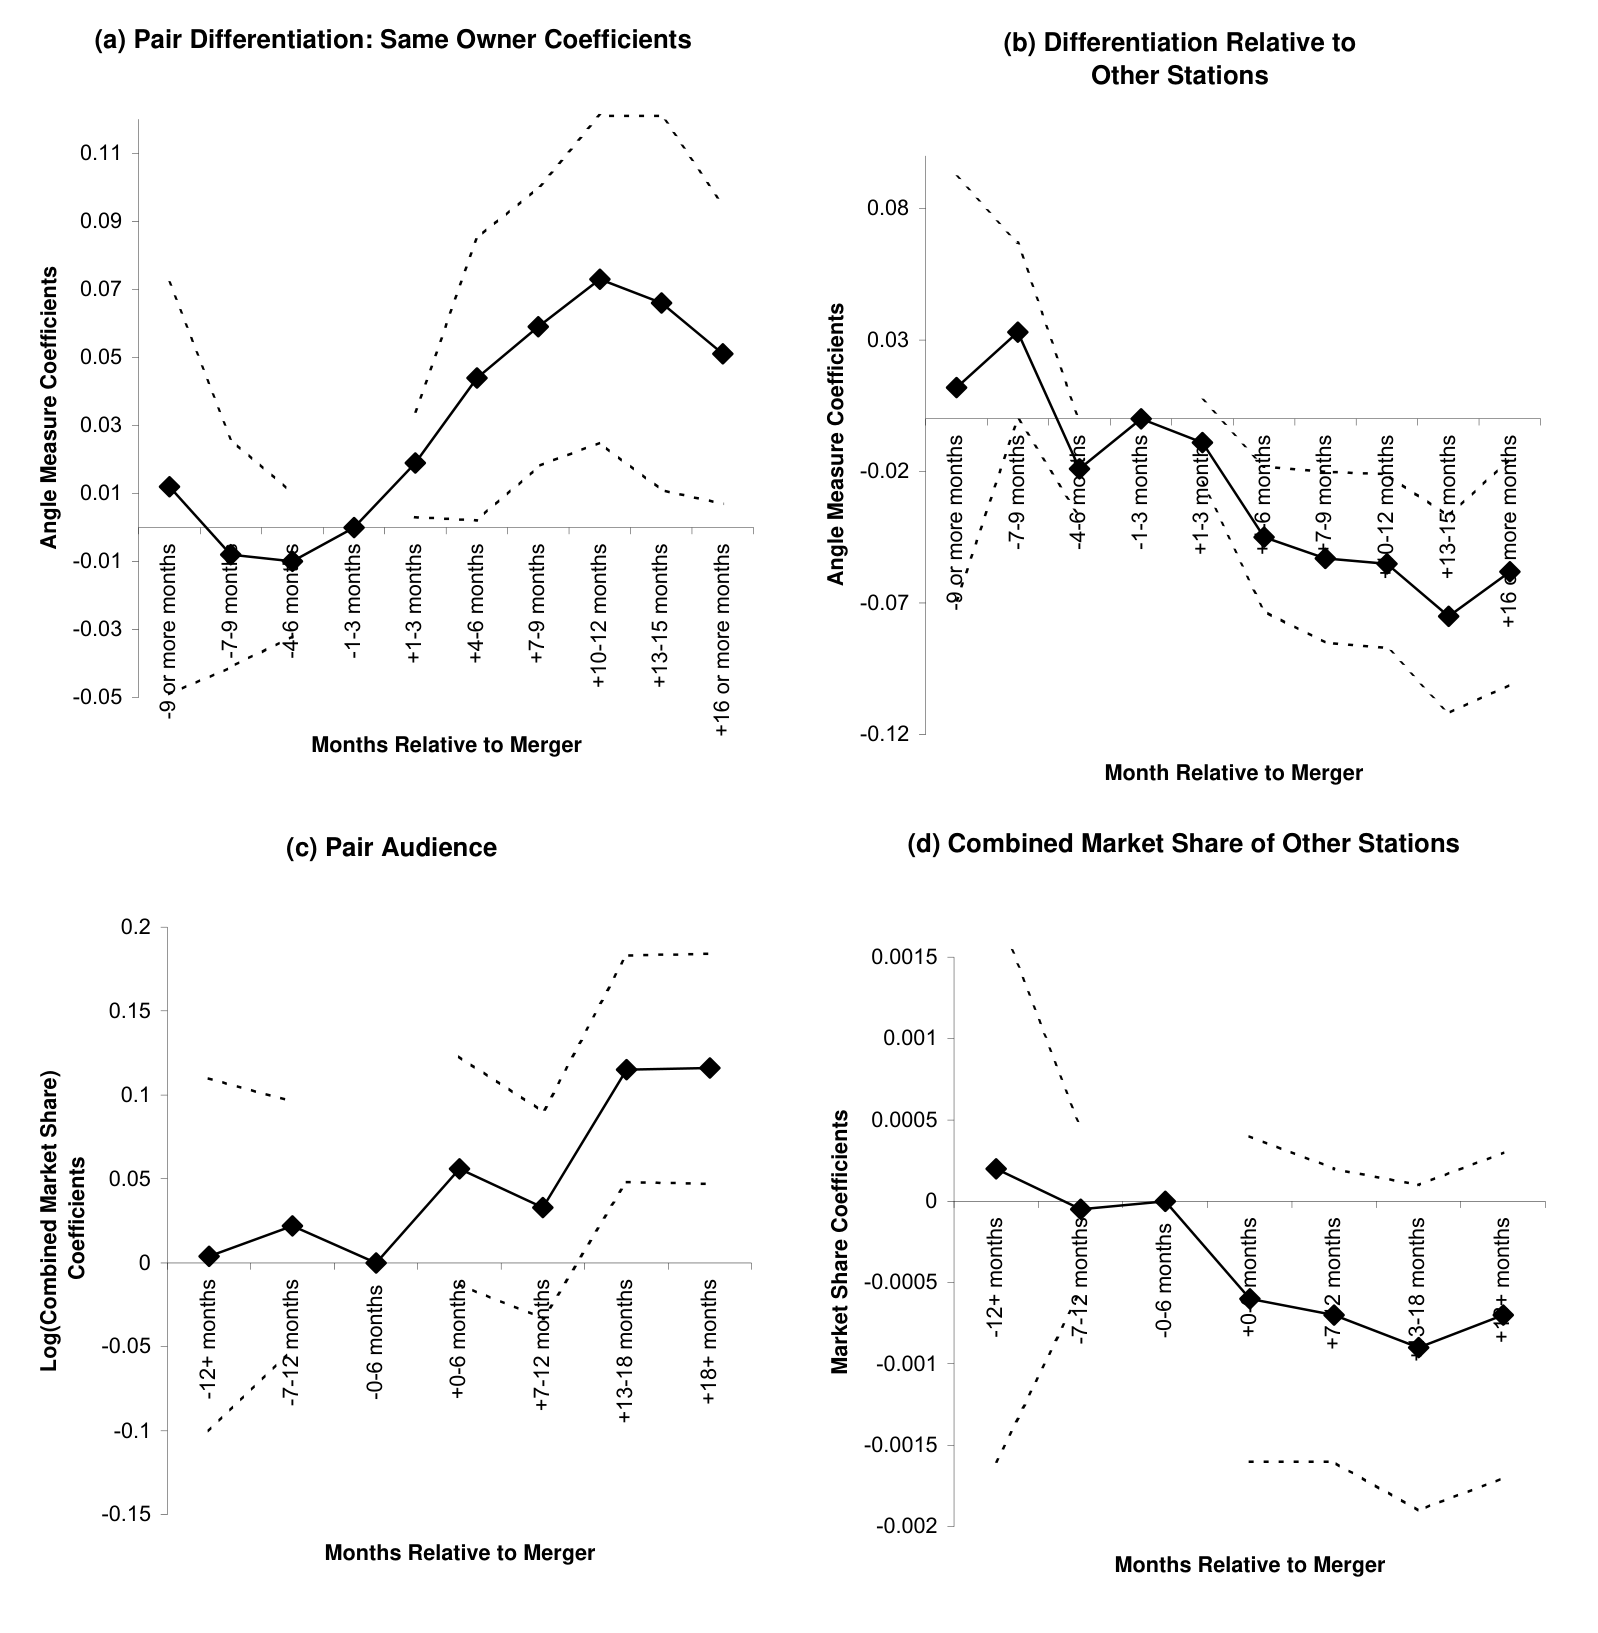
\includegraphics[width=0.84\textwidth]{figures/ch11/sweeting_fig1.png}
\caption{Timing of changes around mergers in music radio. Coefficients on dummies for time relative to the merger, with
95 percent confidence intervals (dashed). Panels (a) and (b) use the angle measure, for differentiation within the
merging pair and between the pair and other stations. Panels (c) and (d) show the log combined share of the pair and
the combined share of other stations. Pairs that ever switch from common to separate ownership are excluded. Source:
\citet{Sweeting2010}, Figure 1.}
\label{fig:11-sweeting}
\end{figure}

\casehead{Robustness}
Section~4 of the paper rules out several alternative explanations. National ownership might raise quality through
economies of scope. In a station-share regression, however, the log number of same-format stations owned nationally has
a coefficient of $-0.0003$ (0.0070), while local common ownership keeps a coefficient of 0.0554 (0.0230) (Table 8).
Changes in signal power or transmitter height do not drive the audience gains. Excluding pairs with technical changes
raises the share coefficient to 0.038 (0.022), and to 0.098 (0.017) when the two quarters after a change are dropped.
Results by format agree in sign in 19 of 21 cases (Table 9). Pairs that merge resemble other pairs before the merger on
three of four outcomes (Table 10). Results are similar for large and small transactions and for mergers and demergers
(Table 11). In data covering all formats and 281 rated markets, owning another station in the same market-format
raises a station's share by 4.6 percent (0.022). The number of owners has no effect on total format listening (Table
12).

\casehead{Interpretation}
The merged firm separates its own stations to reduce cannibalization, as a Hotelling owner without price competition
would. It also moves them toward rivals and takes their listeners. It does not use the new positions to serve
unserved tastes or to soften competition. Three implications follow for merger analysis. Models that hold products fixed will misstate the effects
of mergers, and repositioning may help explain why such models often predict post-merger prices poorly
\citep{Peters2006}. Rivals can be harmed by a merger without synergies, so their complaints do not by themselves
signal that the merger is pro-competitive. This contrasts with the logic of \cref{sec:11-cournot}. Aggregate variety
can stay constant even when the merging firms differentiate, so studies of format counts such as
\citet{BerryWaldfogel2001} see only part of the adjustment. The welfare effect of the repositioning remains open,
since moving closer to rivals transfers listeners without creating variety (\cref{ch:newgoods}).

\casehead{Limitations and contribution}
The study is descriptive and lacks an instrument for ownership. It measures positions with playlists only, ignoring
talk and personality programming. It covers relatively successful music stations in larger markets. The industry is
unusual in ways that \citet[pp.~25--26]{Sweeting2010} lists: horizontal differentiation dominates, listening is
inelastic, price competition through commercials is weak, and playlist changes do not affect costs. The paper's
contribution is a set of stylized facts that structural models of endogenous product choice should match.

Structural merger simulations with repositioning have since followed, each adapted to its industry
\citep[pp.~236--237]{AskerNocke2021}. \citet{LiEtAl2019} study airline mergers. A first-stage entry model, in which a
carrier chooses between nonstop and connecting service on a route, is attached to a nested logit demand model.
\citet{Wollmann2018} also uses a first-stage entry model, to study how a merger changes the product mix in the US
market for commercial vehicles. \citet{Fan2013} lets merging newspapers adjust their prices and three dimensions of
quality. Because the characteristics are continuous, repositioning adds first-order conditions for them to the
pricing conditions of \cref{sec:11-simframework}. \citet{MazzeoSeimVarela2018} add a product-selection stage to a
standard simulation and explore its effects in a range of simulations. \citet{DraganskaMazzeoSeim2009} study
assortment choice more broadly.

These studies agree with Sweeting that a merger can change the incentives to offer particular products, and that
allowing for repositioning changes the estimated effect on consumer welfare. They disagree on the direction of the
bias from ignoring it. Repositioning or entry by a rival adds competitive pressure, while the merged firm's exit from
a product space removes it and adds to the harm. Which force dominates depends on the industry
\citep[p.~237]{AskerNocke2021}.

\subsection{Mergers and capacity investment in the paper industry: Pesendorfer (2003)}\label{sec:11-pesendorfer}

\casehead{Question}
In industries where capacity is the main strategic variable, a merger changes the allocation of capital and the
incentives to invest. A study of short-run prices or outputs can then mismeasure the merger's effects.
\citet{Pesendorfer2003} studies the wave of 31 horizontal mergers in the US paper and paperboard industry between
August 1984 and July 1987. He models capacity investment, uses firms' investment choices before and after the wave to
infer the cost changes that mergers produced, and computes the implied welfare effects. The wave followed the 1984
revision of the Merger Guidelines, which signaled a friendlier stance toward mergers.

\casehead{The investment model}
There are $n$ firms producing a homogeneous good. Firm $i$ starts with capacity $K_i$ and chooses investment $x_i$,
which may be negative (scrapping). Capacity depreciates by the factor $\vartheta \in (0,1)$, so the post-investment
capacity is $\vartheta K_i + x_i$. Adding capacity costs $r(x_i)$, while scrapping is free. Production cost is
$C_i(\cdot)$ with marginal cost $c_i(\cdot)$. Plants run at full capacity, an assumption that fits an industry whose
utilization averaged 93 percent, so industry output is $Q = \sum_j(\vartheta K_j + x_j)$. Firms discount the future by
$\delta \in (0,1)$. Pesendorfer writes $\beta$ for the discount factor and $\delta$ for depreciation, and we rename
both to follow \cref{ch:collusion-theory}. Firm $i$'s payoff is the discounted stream of future profits from the new
capacity, minus investment cost (eq.~(1)):
\begin{equation}\label{eq:11-pes-payoff}
\Pi_i(x) = \frac{\delta}{1 - \delta}\Big[(\vartheta K_i + x_i)\,P\Big(\sum_j(\vartheta K_j + x_j)\Big) - C_i(\vartheta K_i
+ x_i)\Big] - r(x_i)\,\indic\{x_i > 0\}.
\end{equation}
The model is a one-shot investment game. Without depreciation ($\vartheta = 1$) and with linear investment cost, its
equilibrium coincides with that of a dynamic game in which all investment occurs at once.

\begin{proposition}[Equilibrium investment, after \citealp{Pesendorfer2003}, Proposition 1]\label{prop:11-pes-kt}
Let $\mathit{MR}_i = P(Q) + (\vartheta K_i + x_i)P'(Q)$ be firm $i$'s marginal revenue from capacity. Assume that an
equilibrium exists, marginal revenue decreases in own capacity, $c_i$ is nondecreasing, and $r$ is increasing and
convex. In an equilibrium, each firm's investment satisfies
\begin{equation}\label{eq:11-pes-kt}
\begin{aligned}
x_i > 0 &: \quad \frac{\delta}{1 - \delta}\big[\mathit{MR}_i - c_i\big] = r'(x_i),\\
x_i < 0 &: \quad \mathit{MR}_i - c_i = 0,\\
x_i = 0 &: \quad 0 \le \frac{\delta}{1 - \delta}\big[\mathit{MR}_i - c_i\big] \le r'(0),
\end{aligned}
\end{equation}
where $c_i$ is evaluated at $\vartheta K_i + x_i$.
\end{proposition}

\begin{proof}
Holding rivals' choices fixed, $\Pi_i$ is concave in $x_i$ on each side of zero under the stated assumptions. For
$x_i \neq 0$ its derivative is $\frac{\delta}{1-\delta}[\mathit{MR}_i - c_i] - r'(x_i)\indic\{x_i > 0\}$, and an
interior optimum sets it to zero, which gives the first two lines. At $x_i = 0$ the payoff has a kink. The left
derivative is $\frac{\delta}{1-\delta}[\mathit{MR}_i - c_i]$ and the right derivative subtracts $r'(0)$. Zero is
optimal when the left derivative is nonnegative, so scrapping does not pay, and the right derivative is nonpositive, so
investing does not pay. This gives the third line. Pesendorfer writes the three cases compactly as
$x_i\{[\mathit{MR}_i - c_i]\frac{\delta}{1-\delta} - r'(x_i)\indic\{x_i > 0\}\} = 0$ (eq.~(2)).
\end{proof}

Inverting \eqref{eq:11-pes-kt} gives marginal cost as a function of observables (Corollary 2, eq.~(3)):
\begin{equation}\label{eq:11-pes-cost}
c_i = \mathit{MR}_i - \frac{1 - \delta}{\delta}\, r'(x_i)\,\indic\{x_i > 0\} \quad (x_i \neq 0),
\qquad
c_i \in \Big[\mathit{MR}_i - \frac{1 - \delta}{\delta}\, r'(0),\; \mathit{MR}_i\Big] \quad (x_i = 0).
\end{equation}
The right-hand side depends on industry capacity and investment, the firm's own capacity and investment, demand and
the investment cost function. Marginal revenue falls with own capacity. So for a given capacity, a firm that invests
more must have a lower marginal cost. This is the inference the empirical work exploits: changes in investment after a
merger reveal changes in the merged firm's costs. Investment is measured as $x_i = K_i' - \vartheta K_i$, where $K_i'$
is next period's capacity. With $\vartheta < 1$ a firm that keeps capacity constant invests a positive amount, so the
interval case rarely arises.

\casehead{Merger analysis in a linear example}
To see what the model implies, Pesendorfer specializes it. We follow \cref{sec:11-ssr} and write the demand intercept
as $a$.

\begin{assumption}[Linear investment model]\label{ass:11-pes}
(i) Demand is $P(Q) = a - bQ$. (ii) $\frac{\delta}{1 - \delta} = \vartheta = 1$. (iii) Unmerged firms have constant
marginal cost $c$, and the merged firm has constant marginal cost $c_m$. (iv) Investment cost is linear, $r(x) = rx$.
(v) Initial capacities are at Cournot levels, $K_i = K^c \equiv \frac{a - c}{b(n + 1)}$.
\end{assumption}

Under (ii) the payoff is one period's profit minus investment cost. Before the merger, all firms hold $K^c$, the price
is $P^0 = c + \frac{a - c}{n + 1}$, each firm earns $\frac{(a - c)^2}{b(n + 1)^2}$, and no firm wants to invest or scrap.
Two firms then merge, and the merged firm $m$ holds $2K^c$.

\begin{proposition}[A profitable merger without synergies]\label{prop:11-pes-profit}
Let \cref{ass:11-pes} hold with $c_m = c$, and suppose $\frac{a - c}{2(n + 1)} \le r$. Then the post-merger game has an
equilibrium in which the merged firm scraps $\frac{K^c}{2}$ and no outsider invests. The price rises to $c +
\frac{3}{2}\,\frac{a - c}{n + 1}$, and the merging firms' joint profit rises by $\frac{1}{4b}\big(\frac{a - c}{n +
1}\big)^2 > 0$.
\end{proposition}

\begin{proof}
Use $b(n + 1)K^c = a - c$ throughout. Suppose outsiders choose $x_i = 0$ and the merged firm chooses $x_m$. Industry
output is $nK^c + x_m$. An outsider's marginal revenue minus cost is
\begin{equation*}
\mathit{MR}_i - c = a - c - b(nK^c + x_m) - bK^c = (a - c) - b(n + 1)K^c - b\,x_m = -b\,x_m .
\end{equation*}
The merged firm's is
\begin{equation*}
\mathit{MR}_m - c = a - c - b(nK^c + x_m) - b(2K^c + x_m) = -\frac{a - c}{n + 1} - 2b\,x_m .
\end{equation*}
This is negative at $x_m = 0$, so the merged firm scraps until $\mathit{MR}_m = c$:
\begin{equation*}
x_m = -\frac{a - c}{2b(n + 1)} = -\frac{K^c}{2}.
\end{equation*}
Its payoff is concave, and investing is never optimal because $\mathit{MR}_m - c - r < 0$ for $x_m \ge 0$. Given
$x_m$, each outsider has $\mathit{MR}_i - c = \frac{a - c}{2(n + 1)} \ge 0$, so scrapping does not pay. Investing
does not pay if this gain is at most $r$, which is the stated condition. So $x_i = 0$ is a best response.

Industry output is $\big(n - \frac{1}{2}\big)K^c$, and the margin is
\begin{equation*}
P - c = (a - c) - \Big(n - \frac{1}{2}\Big)\frac{a - c}{n + 1} = \frac{3}{2}\,\frac{a - c}{n + 1}.
\end{equation*}
The merged firm sells $\frac{3}{2}K^c$, so its profit is $\frac{3}{2}\frac{a - c}{n + 1}\times\frac{3}{2}\frac{a - c}{b(n
+ 1)} = \frac{9}{4b}\big(\frac{a - c}{n + 1}\big)^2$. Before the merger the two firms earned $\frac{2}{b}\big(\frac{a -
c}{n + 1}\big)^2$. The difference is $\frac{1}{4b}\big(\frac{a - c}{n + 1}\big)^2$.
\end{proof}

\citet[Remark 3]{Pesendorfer2003} states the result under the condition $n + 1 > \frac{a - c}{r}$, which implies the
weaker condition used above. The mechanism is the asymmetry between expanding and contracting capacity. The merged firm
can withdraw capacity at no cost, while outsiders would have to pay $r$ per unit to fill the gap. If $r = 0$, outsiders
expand freely, every firm sets $\mathit{MR} = c$, and the post-merger outcome is Cournot with $n - 1$ firms. A
two-firm merger is then unprofitable for $n \ge 3$ (\cref{prop:11-ssr}). For any $r > 0$, however, a profitable merger
exists once $n$ is large enough \citep[p.~7, n.~6]{Pesendorfer2003}.

\begin{example}[Investment makes the merger profitable]\label{ex:11-pes}
Let $a = 10$, $b = 1$, $c = 2$, $n = 4$ and $r = 1$. Cournot capacities are $K^c = 1.6$, the price is $P^0 = 3.6$ and
each firm earns 2.56. After a merger of two firms, the merged firm scraps 0.8 units, outsiders' marginal gain from
investing is $0.8 < r$, and the price rises to 4.4. The merged firm earns $2.4 \times 2.4 = 5.76$, a gain of 0.64 over
the combined 5.12. Pesendorfer's sufficient condition would require $r > 1.6$, so the example lies in the region
covered only by the weaker condition. With costless expansion the outcome would be Cournot with three firms, a price of
4.0 and a merged profit of 4.0, a loss of 1.12. Costly expansion makes the merger profitable precisely because rivals
do not replace the withdrawn capacity, so consumers face a higher price than in the Cournot benchmark.
\end{example}

The example shows a general feature. The post-merger margin is $\frac{3}{2}\frac{a - c}{n + 1}$, while the Cournot
margin with $n - 1$ firms is $\frac{a - c}{n}$. The first is larger whenever $n > 2$. Pesendorfer's three remaining
remarks describe what investment reveals about costs and welfare.

\begin{proposition}[Investment and merger cost savings, Remarks 4 to 6]\label{prop:11-pes-remarks}
Let \cref{ass:11-pes} hold.
\begin{enumerate}[label=(\alph*)]
  \item If the merged firm does not change its capacity after the merger ($x_m = 0$), then no outsider does either, and
  $2c - P^0 - r \le c_m \le 2c - P^0$. In particular $c_m < c$.
  \item If $c_m = c$, industry capacity falls and the merger reduces total welfare.
  \item If $x_m = 0$, consumer surplus is unchanged and total welfare rises.
\end{enumerate}
\end{proposition}

\begin{proof}
(a) With $x_m = 0$ and symmetric outsiders, an outsider's marginal gain is $-b(n - 1)x_i$. A positive $x_i$ would
require this to equal $r > 0$, and a negative $x_i$ would require it to equal zero, so $x_i = 0$. The merged firm's
marginal revenue at $x_m = 0$ is $a - b(n + 2)K^c = P^0 - 2(P^0 - c) = 2c - P^0$. Zero investment requires $0 \le
\mathit{MR}_m - c_m \le r$, which is the stated band. Since $P^0 > c$, $c_m \le 2c - P^0 < c$.

(b) Suppose instead that total investment $X = \sum_j x_j$ is positive. An outsider's marginal gain is $-b(X + x_i)$,
which cannot equal $r > 0$ when $x_i > 0$ and $X > 0$, so $x_i \le 0$. The merged firm's is $-\frac{a - c}{n + 1} -
b(X + x_m)$, which is negative when $x_m > 0$ and $X > 0$, so $x_m \le 0$. Then $X \le 0$, a contradiction. If $X = 0$,
the merged firm's marginal gain at any $x_m \ge 0$ is negative, so it scraps. Outsiders would then have to invest, but
an outsider with $x_i > 0$ has marginal gain $-b\,x_i < 0 < r$. Hence $X < 0$. Output falls below the pre-merger level, at which price exceeds the common marginal cost,
so total surplus falls.

(c) By part (a), output is unchanged, so price and consumer surplus are unchanged. Producer surplus rises because the
merged firm produces the same capacity at $c_m < c$.
\end{proof}

Part (a) connects the investment model to \cref{prop:11-synergy}. If nobody adjusts capacity, output and price are
unchanged, so the merger must be at least price-neutral. The merged firm's cost must then lie at or below the
price-neutral level $2c - P^0$ of the Cournot analysis. In \cref{ex:11-pes}, $2c - P^0 = 0.4$, an 80 percent cost
reduction. Unchanged investment after a merger thus reveals large savings. Consumer surplus and producer surplus
are defined as usual (eqs.~(4)--(5)):
\begin{equation}\label{eq:11-pes-welfare}
\mathit{CS} = \int_0^Q P(z)\,\dd z - Q\,P(Q), \qquad
\mathit{PS} = \sum_i\big[K_iP(Q) - C_i(K_i) - r(x_i)\indic\{x_i > 0\}\big].
\end{equation}

\casehead{Data}
Plant-level annual capacities by product for 1978--1992 come from Lockwood's Directory of the Paper and Allied Trades,
supplemented by Census price data. Products fall into nine categories: newsprint, packaging papers, groundwood printing,
coated papers, uncoated papers, other papers, tissue, linerboard and boxboard. Products within a category are largely
homogeneous, and about 80 percent of capacity is in plants producing a single category, so each category is treated as
a separate market. Newsprint is dropped because about half of US newsprint capacity is imported from Canada. The
geographic market is the United States, with exports of about 15 percent of production and imports of about 12 percent
in 1991.

Table~1 of the paper summarizes the industry. The average number of firms per category fell from 70.6 in 1978 to 60.4
in 1992. The five largest firms held on average 56.1 percent of capacity in 1992, from 41 percent in newsprint to 75
percent in tissue. Capacity grew by about 20 percent over the period, at about 0.7 percent a year before 1987 and 2.4
percent after. About 40 percent of capacity expansions at existing firms came through horizontal acquisitions, and about
40 percent of the 819 plants were involved in at least one merger. The 1984--1987 wave included Champion
International's acquisition of St.~Regis (\$1.8 billion), Jefferson Smurfit's of Container Corporation (\$1.2 billion)
and International Paper's of Hammermill (\$1.1 billion). The Federal Trade Commission blocked James River's acquisition
of Barlow Rand in February 1988. Every category had at least one merger in the wave.

\casehead{Descriptive evidence}
Merged firms' outcomes vary widely. Table~3 regresses the merged firm's share, relative to its share at the merger, on
time since the merger and its square. In the pooled data the coefficients are $-3.66$ ($t = 5.9$) and $0.35$ ($t =
3.0$), with $R^2 = 0.04$ and 1,112 observations. The share falls to about 90 percent of its initial level after about five
years and then recovers. About two-thirds of acquirers lose share and one-third gain. Probit models of annual investment
decisions on 9,352 firm-years show that a merger raises the probability of changing capacity. The coefficient on the
relative size of the acquired firm is 0.7589 ($t = 3.5$), and the coefficient on an acquisition two to five years
earlier is 0.6004 ($t = 2.4$). The effect works mostly through scrapping, with coefficients of 0.8017 ($t = 2.9$) and 0.7027 ($t = 2.2$), while
the effects on investing are positive but insignificant (Table 4). About 24 percent of firms change capacity in a given
year, three-quarters of them upward.

\casehead{Estimation}
Costs are estimated in two steps for three-year windows before and after the wave, since new capacity takes two to
three years to become usable. The wave is assumed to have been unanticipated when the earlier investments were made.
The first step estimates constant-elasticity inverse demand for each category,
\begin{equation}\label{eq:11-pes-demand}
\ln P_t = \alpha_x x_t + \gamma \ln Q_t + u_t, \qquad u_t = \varrho\, u_{t-1} + v_t, \quad |\varrho| < 1,
\end{equation}
with gross domestic product as the demand shifter $x_t$ and wages of paper workers as the instrument for output. The
second step computes each firm's marginal revenue $\widehat{\mathit{MR}}_i = \hat P(Q) + \hat P'(Q)K_i$ and recovers its
marginal cost from \eqref{eq:11-pes-cost}. The discount factor is 0.95 per year. The investment cost has a linear and
a quadratic term calibrated to reported costs of investment projects in the trade press. The base specification sets
the depreciation factor to 0.999 with linear coefficient 26.50 and quadratic coefficient 0.005, and four alternatives
vary these values.

\casehead{Cost results}
Acquiring firms have lower estimated marginal costs than unmerged firms before the wave, and the gap widens after it.
In groundwood printing, for instance, the median difference between acquiring and unmerged firms grows from \$4.39 to
\$8.01 per ton, and the mean difference from \$6.97 to \$12.87 (Table 5A). The median gap widens in all eight categories
and the mean gap in seven, the exception being boxboard. To separate merger effects from industry-wide cost changes,
Pesendorfer assigns each cost estimate its percentile in the distribution of unmerged firms' costs, before and after
the wave. \Cref{fig:11-pesendorfer} shows the result. About 90 percent of acquiring firms move to lower percentiles,
and about 10 percent do not. The Champion-St.~Regis merger is an example of expected synergies that did not
materialize.

\begin{figure}[htbp]
\centering
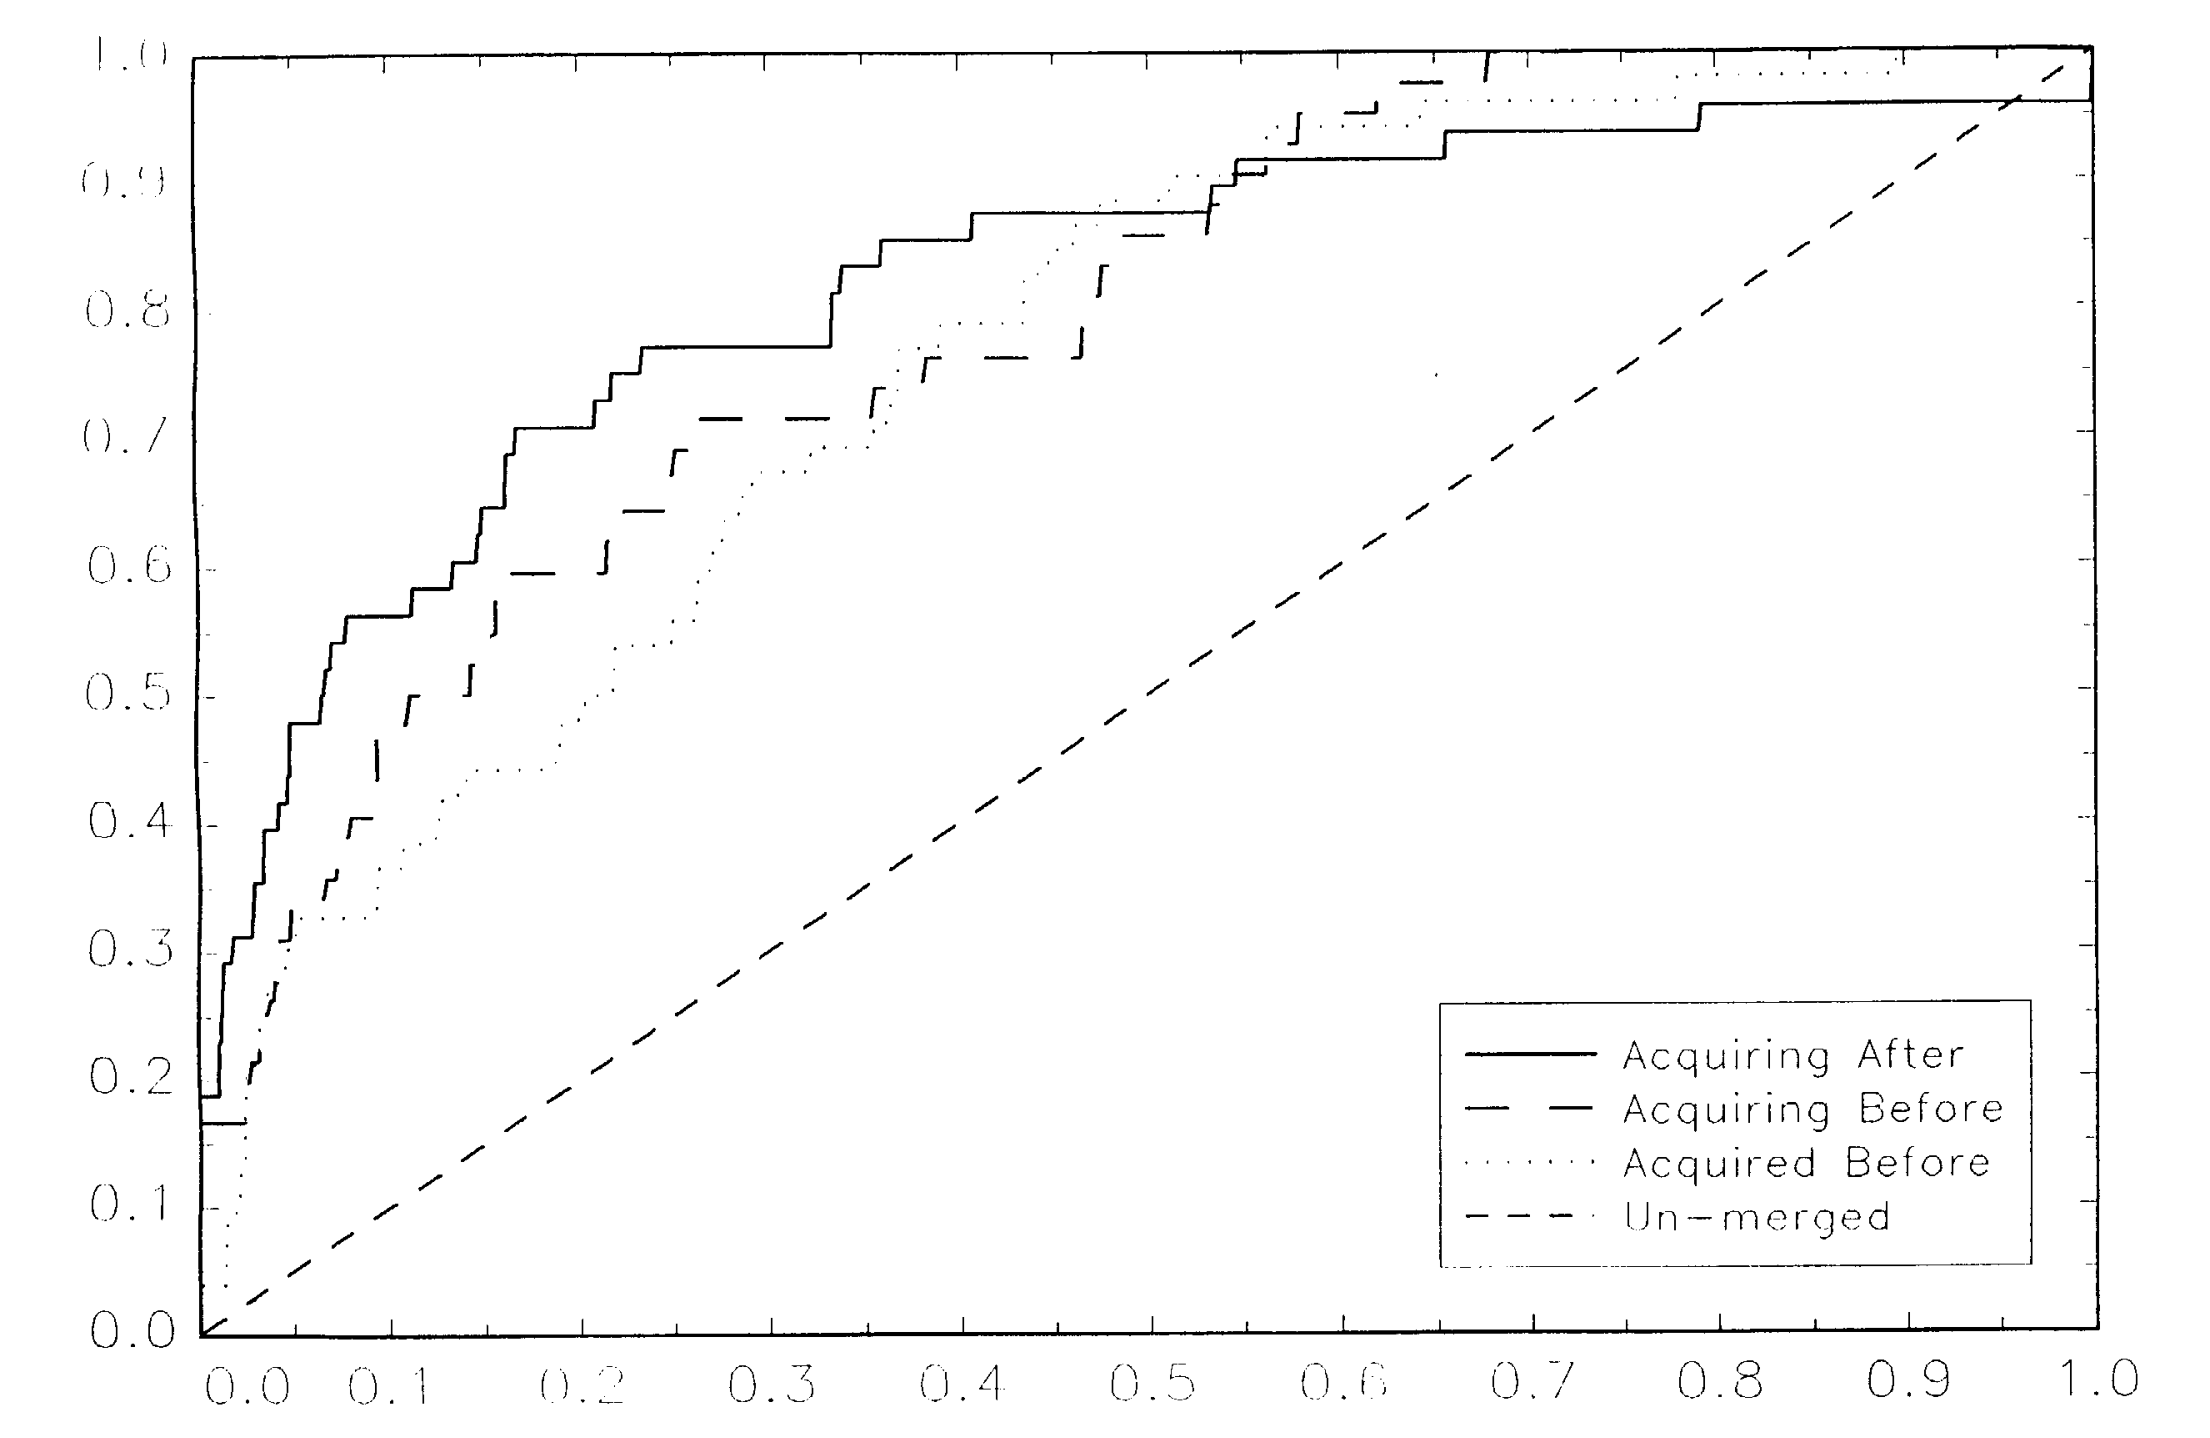
\includegraphics[width=0.72\textwidth]{figures/ch11/pesendorfer_fig2.png}
\caption{Distribution of estimated marginal costs, pooled across paper categories. Each firm's cost is expressed as
its percentile in the cost distribution of unmerged firms (horizontal axis). The curves are cumulative distribution
functions (vertical axis) for acquiring firms after and before the merger wave and for acquired firms before it. The dashed diagonal
is the distribution of unmerged firms. Curves farther above the diagonal indicate lower relative costs. The image is
rotated from the working-paper version. Source: \citet{Pesendorfer2003}, Figure 2.}
\label{fig:11-pesendorfer}
\end{figure}

\casehead{Welfare}
For the counterfactual without mergers, each merging firm's cost is projected to its post-wave level using its
percentile in the unmerged distribution. The merged firm is replaced by its components with these costs, the
investment equilibrium of \eqref{eq:11-pes-kt} is recomputed, and the changes in consumer and producer surplus follow
from \eqref{eq:11-pes-welfare}. Standard errors come from repeated draws of the projection error. \Cref{tab:11-pesendorfer}
reproduces the base specification.

\begin{table}[htbp]
\centering
\caption{Welfare effects of the 1984--1987 paper merger wave (thousands of 1986 dollars)}
\label{tab:11-pesendorfer}
\begin{threeparttable}
\small
\begin{tabular}{@{}lrrrrr@{}}
\toprule
Category & \makecell[r]{Total\\ welfare} & \makecell[r]{Consumer\\ surplus} & \makecell[r]{Producer\\ surplus} &
\makecell[r]{Merged\\ firms} & \makecell[r]{Unmerged\\ firms} \\
\midrule
Packaging papers & 61,440 & 9,499 & 51,940 & 57,090 & $-5{,}149$ \\
 & (14,635) & (6,174) & (9,145) & (12,135) & (3,494) \\
Groundwood printing & 1,736 & 3,132 & $-1{,}395$ & 419 & $-1{,}815$ \\
 & (12,187) & (6,380) & (6,393) & (9,207) & (3,213) \\
Coated papers & 9,617 & 10,604 & $-987$ & 5,708 & $-6{,}695$ \\
 & (11,036) & (11,241) & (3,950) & (7,321) & (7,118) \\
Uncoated papers & 16,826 & 21,277 & $-4{,}451$ & 9,747 & $-14{,}198$ \\
 & (21,463) & (10,197) & (13,863) & (18,991) & (7,234) \\
Other papers & 31,166 & 4,888 & 26,278 & 28,832 & $-2{,}554$ \\
 & (4,094) & (1,713) & (2,479) & (3,439) & (1,036) \\
Tissue & 298,692 & 96,089 & 202,604 & 242,905 & $-40{,}301$ \\
 & (14,676) & (7,950) & (6,815) & (11,952) & (5,240) \\
Boxboard & 412 & $-22{,}098$ & 22,510 & 11,832 & 10,679 \\
 & (16,381) & (8,594) & (8,412) & (12,233) & (4,235) \\
Linerboard & 163,587 & 90,203 & 73,384 & 112,771 & $-39{,}386$ \\
 & (82,962) & (64,079) & (52,942) & (60,261) & (28,788) \\
\midrule
Sum over categories & 583,476 & 213,594 & 369,883 & 469,304 & $-99{,}419$ \\
Range over five specifications & 454,483 to & $-58{,}555$ to & 244,271 to & & \\
 & 583,476 & 213,594 & 527,289 & & \\
\bottomrule
\end{tabular}
\begin{tablenotes}[flushleft]
\footnotesize
\item Notes: Reproduced from \citet[Table 6, specification (1): depreciation factor 0.999, linear investment-cost
coefficient 26.50, quadratic 0.005]{Pesendorfer2003}, working-paper version. Standard deviations from the projection
error in parentheses. The table reports categories only. The sums and ranges are our calculations from all five
columns of the table. The other specifications use (0.950, 26.50, 0.005), (0.999, 36.50, 0.007), (0.999, 53.00, 0)
and (0.999, 0, 0.010).
\end{tablenotes}
\end{threeparttable}
\end{table}

Summing over categories, the wave raised total welfare by \$583.5 million in the base specification, with \$213.6
million going to consumers and \$369.9 million to producers. The sums across the five specifications range from \$454
million to \$583 million for total welfare and from \$244 million to \$527 million for producer surplus. The text of the
paper gives a consumer range of \$58 million to \$210 million, while the table's columns sum to between $-\$58.6$ million
and \$213.6 million.
Merged firms gained \$469.3 million and unmerged firms lost \$99.4 million.
The text reports the merged firms' gain as \$468.3 million in two places and \$469.3 million in a third. The table
sums to the latter. The paper describes the packaging-paper figure as an increase in annual total welfare
\citep[p.~19]{Pesendorfer2003}, so the totals are best read as annual flows. Gains to merged firms are positive in every
category in the base specification. Pesendorfer states that these gains are positive in six of eight categories, with
insignificant losses in some specifications for groundwood printing and boxboard \citep[p.~21]{Pesendorfer2003}. His
Table 6 also shows insignificant losses in one specification each for uncoated papers ($-703$ thousand) and
linerboard ($-26{,}638$ thousand). Only packaging, coated, other papers and tissue show gains in every specification.
Pesendorfer reads the positive gains as support for the model, since profitability was not imposed in estimation.

\casehead{Interpretation and critiques}
The welfare gains rest on estimated cost reductions, and their distribution deserves attention. Tissue alone accounts
for 51 percent of the total welfare gain and 52 percent of the merged firms' gain. The tissue category had a single
acquiring firm (Table 2), whose estimated cost advantage over the median unmerged firm grew from \$5.71 to \$143.04 per
ton (Table 5A). The headline number thus depends heavily on one firm's inferred cost decline. More generally, marginal
costs are residuals of a first-order condition, so any misspecification of demand, of the investment cost function or
of conduct is loaded into the cost estimates. The model is static and assumes the wave was unanticipated. It treats
each category as a national homogeneous-good market with full utilization. The percentile projection assumes that, absent
mergers, each firm would have kept its relative position. Mergers are taken as given, so firms that merged may differ
from others in ways that also explain later cost changes.

\casehead{Contribution}
The paper shows that the investment channel can reverse two conclusions of static Cournot theory. Mergers without
synergies can be profitable, and the price effect of a merger depends on rivals' ability to add capacity. It also
shows how revealed investment behavior can identify merger efficiencies, an idea that complements the retrospective
price studies of \cref{sec:11-retro}. Dynamic models of mergers with investment, such as \citet{BerryPakes1993} and
\citet{Gowrisankaran1999}, develop the same concerns with richer state spaces.

\section{Merger policy with merger choice}\label{sec:11-policy}

The standard approach to merger review evaluates each proposed merger on its own. An authority with a consumer surplus
standard approves a merger if and only if it does not lower consumer surplus. This rule ignores that firms choose which
merger to propose, while the authority sees only the proposal. \citet{NockeWhinston2013} show that the choice changes
the optimal policy. If firms prefer larger mergers for reasons unrelated to consumers, the authority should hold larger
mergers to a stricter standard. \citet{Lyons2003} first identified the problem. \citet{ArmstrongVickers2010} analyze
delegated choice among projects that are ex ante identical. \citet{NockeWhinston2010} show that a myopic consumer
surplus standard is optimal in a dynamic setting when possible mergers are disjoint, that is, involve different firms.
We follow the working-paper version of \citet{NockeWhinston2013}, whose numbering may differ from the published
article.

\subsection{The model}\label{sec:11-nw-model}

Firms $i \in \mathcal{N} = \{0, 1, \dots, N\}$ produce a homogeneous good with constant marginal costs $c_i$ and
compete in quantities. Inverse demand $P(Q)$ satisfies, for all $Q$ with $P(Q) > 0$,
\begin{equation}\label{eq:11-nw-ass}
P'(Q) < 0, \qquad P'(Q) + QP''(Q) < 0, \qquad \lim_{Q \to \infty}P(Q) = 0 .
\end{equation}
These conditions imply a unique Cournot equilibrium that is stable: each best response $b_i(Q_{-i})$ has slope in
$(-1, 0)$, so if some firms want to produce less, industry output falls. All firms are active, and the pre-merger
outputs satisfy $P(Q^0) + P'(Q^0)q_i^0 = c_i$. Write $P^0 = P(Q^0)$, $s_i^0 = \frac{q_i^0}{Q^0}$ and $\pi_i^0 = (P^0 -
c_i)q_i^0$.

Firm 0, the acquirer, can merge with one target $k \in \mathcal{K} = \{1, \dots, K\}$. Targets are ordered by decreasing
cost, $c_1 > c_2 > \dots > c_K$, so a higher $k$ means a larger pre-merger share. We call merger $k$ \emph{larger}
than merger $j$ if $k > j$. The change in the naively computed Herfindahl index, which keeps all shares fixed and adds
the merging shares, is
\begin{equation}\label{eq:11-nw-hhi}
\Delta\HHI^{naive}(M_k) = (s_0^0 + s_k^0)^2 - (s_0^0)^2 - (s_k^0)^2 = 2 s_0^0 s_k^0 ,
\end{equation}
the formula of \eqref{eq:11-dhhi}. A larger merger thus has a larger naive increase in concentration.

Merger $k$ is feasible with probability $\phi_k \in (0, 1]$, independently across targets. If feasible, it yields a
post-merger marginal cost $\bar c_k$ drawn from a distribution $G_k$ with support $[c^L, c_k^H]$ and no mass points. A
feasible merger is $M_k = (k, \bar c_k)$. After merger $M_k$ the outputs solve $P(Q(M_k)) + P'(Q(M_k))q_i(M_k) = c_i$
for nonmerging firms and the same condition with $\bar c_k$ for the merged firm. All firms remain active. The changes in
consumer surplus and in the merging parties' joint (bilateral) profit are
\begin{equation}\label{eq:11-nw-changes}
\Delta \mathit{CS}(M_k) = \int_0^{Q(M_k)}P(z)\,\dd z - P(Q(M_k))Q(M_k) - \mathit{CS}^0,
\qquad
\Delta\Pi(M_k) = \pi_k(M_k) - (\pi_0^0 + \pi_k^0).
\end{equation}
A merger is \emph{CS-neutral} if $\Delta\mathit{CS} = 0$, CS-increasing if it is positive, CS-decreasing if it is
negative, and CS-nondecreasing if it is not CS-decreasing. The status quo $M_0$ gives zero changes. Let $\mathcal{F}$
be the realized set of feasible mergers, including $M_0$.

The timing has four stages. The authority commits to an approval set $\mathcal{A} = \{M_k : \bar c_k \in
\mathcal{A}_k\} \cup \{M_0\}$, where each $\mathcal{A}_k \subseteq [c^L, c_k^H]$ is a union of closed intervals. Nature
draws $\mathcal{F}$. Firms bargain over which merger to propose. The authority approves the proposal if it lies in
$\mathcal{A}$, and firms compete. The authority observes every characteristic of the proposed merger but nothing about
mergers that are not proposed, and only one merger can be proposed.

Bargaining follows the offer game of \citet{Segal1999}. Firm 0 makes a take-it-or-leave-it offer of a price $t_k$ to one
target. Setting $t_k$ to make the target indifferent, firm 0 captures the whole bilateral gain $\Delta\Pi(M_k)$. The
proposed merger is therefore
\begin{equation}\label{eq:11-nw-proposal}
M^*(\mathcal{F}, \mathcal{A}) =
\begin{cases}
\argmax_{M_k \in \mathcal{F} \cap \mathcal{A}} \Delta\Pi(M_k) & \text{if } \max_{M_k \in \mathcal{F} \cap \mathcal{A}}
\Delta\Pi(M_k) > 0,\\
M_0 & \text{otherwise.}
\end{cases}
\end{equation}
The authority chooses $\mathcal{A}$ to maximize $\E_{\mathcal{F}}\big[\Delta\mathit{CS}(M^*(\mathcal{F}, \mathcal{A}))
\big]$. One assumption avoids trivial cases. Each merger's cost support contains CS-increasing and CS-nonincreasing
outcomes, $\Delta\mathit{CS}(k, c_k^H) \le 0 < \Delta\mathit{CS}(k, c^L)$.

\subsection{Three lemmas on the shape of merger outcomes}\label{sec:11-nw-lemmas}

Because the good is homogeneous, a merger raises consumer surplus if and only if it raises industry output. The first
lemma characterizes CS-neutral mergers. It restates \cref{prop:11-synergy,cor:11-neutral-profit} in the notation of
this section.

\begin{lemma}[CS-neutral mergers]\label{lem:11-nw1}
Suppose merger $M_k$ is CS-neutral. Then (i) no nonmerging firm changes its output, and the merged firm produces
$q_0^0 + q_k^0$. (ii) The merged firm's margin equals the sum of the partners' margins,
\begin{equation}\label{eq:11-nw-neutral}
P^0 - \bar c_k = (P^0 - c_0) + (P^0 - c_k), \quad\text{so}\quad \bar c_k = \hat c_k \equiv c_k - (P^0 - c_0) <
\min\{c_0, c_k\}.
\end{equation}
(iii) The merger is profitable, $\Delta\Pi(M_k) > 0$. (iv) It raises aggregate profit.
\end{lemma}

\begin{proof}
A CS-neutral merger leaves $Q$, and hence $P$ and $P'$, unchanged. Each nonmerging firm's first-order condition then
gives the same output, and the merged firm produces the rest, $q_0^0 + q_k^0$. Its first-order condition is $P^0 +
P'(Q^0)(q_0^0 + q_k^0) = \bar c_k$. Adding the partners' pre-merger conditions gives $2P^0 + P'(Q^0)(q_0^0 + q_k^0) =
c_0 + c_k$. Subtracting the first equation from the second gives $P^0 = c_0 + c_k - \bar c_k$, which is
\eqref{eq:11-nw-neutral}. Part (iii) is \cref{cor:11-neutral-profit}: the merged profit exceeds $\pi_0^0 + \pi_k^0$ by
$(P^0 - c_0)q_k^0 + (P^0 - c_k)q_0^0 > 0$. For (iv), nonmerging firms' profits are unchanged because their prices and
outputs are unchanged.
\end{proof}

\begin{lemma}[Lower post-merger cost]\label{lem:11-nw2}
Conditional on merger $M_k$, a lower $\bar c_k$ raises industry output, consumer surplus and the merged firm's profit.
\end{lemma}

\begin{proof}
Summing the $N$ post-merger first-order conditions gives $NP(Q) + QP'(Q) = \bar c_k + \sum_{i \neq 0, k}c_i$. The
left side decreases in $Q$, because its derivative is $(N + 1)P' + QP'' < 0$ by \eqref{eq:11-nw-ass}. A lower
$\bar c_k$ lowers the right side, so $Q$ rises, and so does consumer surplus. For the profit, define the
\emph{cumulative best reply} $\tilde q(Q; c) = -\frac{P(Q) - c}{P'(Q)}$, the output at which a firm with cost $c$
satisfies its first-order condition when industry output is $Q$. Its derivative in $Q$ is
\begin{equation*}
\frac{\partial\tilde q}{\partial Q} = -1 + \frac{(P - c)P''}{(P')^2} = -1 - \frac{\tilde q\,P''}{P'} =
-\frac{P' + \tilde q P''}{P'} < 0,
\end{equation*}
using $P - c = -P'\tilde q$ and $P' + qP'' < 0$ for $q \le Q$. Nonmerging outputs $\tilde q(Q; c_i)$ therefore fall
when $\bar c_k$ falls. The merged firm's profit is $\max_q[P(Q_{-m} + q) - \bar c_k]q$, where $Q_{-m}$ is rivals'
output. By the envelope theorem its derivative in $\bar c_k$ is $-q_m + q_m P'(Q)\frac{dQ_{-m}}{d\bar c_k}$. Both terms
are negative, since $P' < 0$ and rivals' output rises with $\bar c_k$.
\end{proof}

Lemma~\ref{lem:11-nw2} implies that merger $M_k$ is CS-increasing if $\bar c_k < \hat c_k$ and CS-decreasing if
$\bar c_k > \hat c_k$. The third lemma is the key to the paper. It shows that firms' proposal incentives are biased
toward larger mergers.

\begin{lemma}[Firms prefer larger mergers]\label{lem:11-nw3}
Suppose mergers $M_j$ and $M_k$, with $k > j \ge 1$, induce the same nonnegative change in consumer surplus. Then the
larger merger induces a larger gain in bilateral profit: $\Delta\Pi(M_k) > \Delta\Pi(M_j) > 0$.
\end{lemma}

\begin{proof}
Each firm's first-order condition gives $P - c_i = -P' q_i$, so its profit is
\begin{equation}\label{eq:11-nw-profit}
\pi_i = (P - c_i)q_i = -P'(Q)\,\big[\tilde q(Q; c_i)\big]^2 .
\end{equation}
Equal consumer surplus means equal industry output $\bar Q$. Industry output depends only on the sum of active
firms' costs, by the summed first-order condition in the proof of Lemma~\ref{lem:11-nw2}. So both mergers reduce the
partners' combined cost by the same amount, $\gamma \equiv c_k - \bar c_k = c_j - \bar c_j$. Since $\frac{\partial\tilde
q}{\partial c} = \frac{1}{P'}$, the difference in the merged firms' profits is
\begin{align}
\pi_k(M_k) - \pi_j(M_j)
&= -P'(\bar Q)\Big\{\big[\tilde q(\bar Q; c_k - \gamma)\big]^2 - \big[\tilde q(\bar Q; c_j - \gamma)\big]^2\Big\}
\notag\\
&= -P'(\bar Q)\int_{c_j}^{c_k} 2\,\tilde q(\bar Q; c - \gamma)\,\frac{1}{P'(\bar Q)}\,\dd c
= 2\int_{c_k}^{c_j}\tilde q(\bar Q; c - \gamma)\,\dd c . \label{eq:11-nw-diff1}
\end{align}
The same steps applied to pre-merger profits give
\begin{equation}\label{eq:11-nw-diff0}
\pi_k^0 - \pi_j^0 = 2\int_{c_k}^{c_j}\tilde q(Q^0; c)\,\dd c .
\end{equation}
Now consider, for any $c \in [c_k, c_j]$, a merger of firm 0 with a firm of cost $c$ that yields cost $c - \gamma$.
It raises output from $Q^0$ to $\bar Q$, so it weakly lowers each nonmerging firm's output and weakly raises the merging
firms' joint output. Hence
\begin{equation*}
\tilde q(\bar Q; c - \gamma) \ge \tilde q(Q^0; c_0) + \tilde q(Q^0; c) > \tilde q(Q^0; c).
\end{equation*}
The integrand of \eqref{eq:11-nw-diff1} exceeds that of \eqref{eq:11-nw-diff0} at every $c$, so
$\pi_k(M_k) - \pi_j(M_j) > \pi_k^0 - \pi_j^0$. Subtracting $\pi_0^0$ from both merged profits and rearranging gives
$\Delta\Pi(M_k) > \Delta\Pi(M_j)$. Finally, $\Delta\Pi(M_j) > 0$ because a CS-nondecreasing merger has $\bar c_j \le
\hat c_j$, and Lemmas~\ref{lem:11-nw1} and~\ref{lem:11-nw2} imply that it is at least as profitable as the CS-neutral
merger.
\end{proof}

The intuition comes from \eqref{eq:11-nw-profit}. Profit is quadratic in output, so a given cost saving is worth more
to a firm that produces more. To leave consumers equally well off, both mergers need the same absolute cost saving,
and the larger merger applies it to a larger output base. Firms therefore value larger mergers more than consumers do.

Lemmas~\ref{lem:11-nw1} to~\ref{lem:11-nw3} fix the geometry of the problem. Plot each possible outcome of merger $k$
as a point $(\Delta\Pi, \Delta\mathit{CS})$. As $\bar c_k$ varies, the points trace a \emph{merger curve}. Each curve
slopes upward (Lemma~\ref{lem:11-nw2}) and crosses the horizontal axis at a positive profit (Lemma~\ref{lem:11-nw1}).
On and above the axis, the curve of a larger merger lies to the right of the curve of a smaller one
(Lemma~\ref{lem:11-nw3}). An immediate consequence is the following.

\begin{corollary}[\citealp{NockeWhinston2013}, Corollary 1]\label{cor:11-nw}
If two CS-nondecreasing mergers $M_j$ and $M_k$ with $k > j \ge 1$ satisfy $\Delta\Pi(M_k) \le \Delta\Pi(M_j)$, then
$\Delta\mathit{CS}(M_k) < \Delta\mathit{CS}(M_j)$.
\end{corollary}

\begin{proof}
Suppose $\Delta\mathit{CS}(M_k) \ge \Delta\mathit{CS}(M_j)$. By Lemma~\ref{lem:11-nw2} there is a cost $\bar c_k' \ge
\bar c_k$ with $\Delta\mathit{CS}(k, \bar c_k') = \Delta\mathit{CS}(M_j)$. Lemma~\ref{lem:11-nw2} and then
Lemma~\ref{lem:11-nw3} give $\Delta\Pi(M_k) \ge \Delta\Pi(k, \bar c_k') > \Delta\Pi(M_j)$, a contradiction.
\end{proof}

\Cref{fig:11-nw} draws the merger curves for the linear example studied below. The curves are close to parallel in
this example, and the larger merger's curve lies to the right at every nonnegative $\Delta\mathit{CS}$.

\begin{figure}[htbp]
\centering
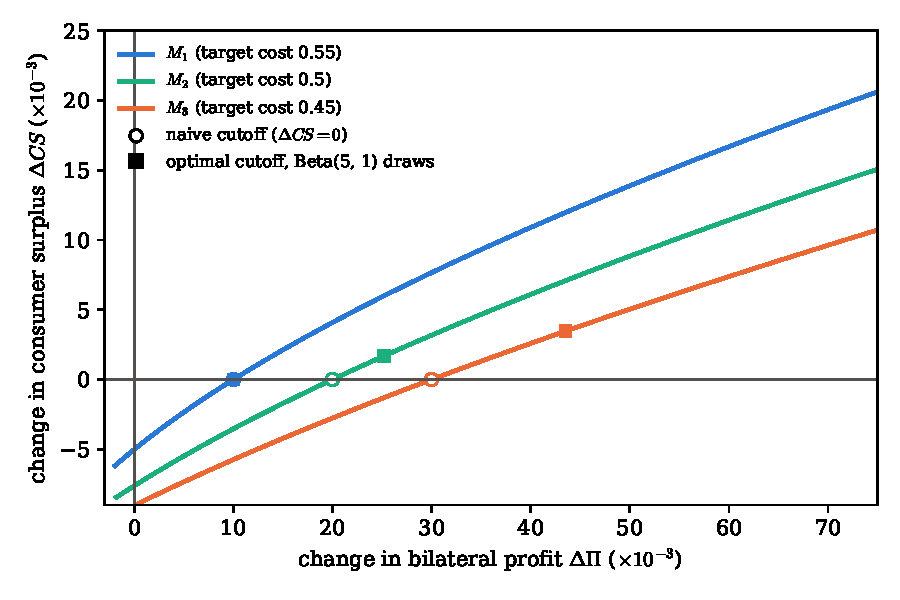
\includegraphics[width=0.78\textwidth]{figures/ch11/nw_curves.pdf}
\caption{Merger curves in $(\Delta\Pi, \Delta\mathit{CS})$ space for Example 2 of \citet{NockeWhinston2013}: inverse
demand $P = 1 - Q$, acquirer cost $c_0 = 0.5$ and targets with costs 0.55, 0.5 and 0.45. Each curve traces the outcomes
of one merger as the post-merger cost $\bar c_k$ varies from 0.2 to slightly above $c_k$. Open circles mark the naive
cutoffs, at which $\Delta\mathit{CS} = 0$. Squares mark the optimal cutoffs when post-merger costs follow the Beta(5, 1)
distribution described in the text. Our computation.}
\label{fig:11-nw}
\end{figure}

\subsection{The optimal approval policy}\label{sec:11-nw-optimal}

For a policy $\mathcal{A}$, let $\bar a_k = \max\mathcal{A}_k$ be the highest approved cost for target $k$. The merger
$(k, \bar a_k)$ is the \emph{marginal merger}, and $\underline{\Delta\mathit{CS}}_k = \Delta\mathit{CS}(k, \bar a_k)$ and
$\underline{\Delta\Pi}_k = \Delta\Pi(k, \bar a_k)$ are the lowest consumer surplus and profit changes among approved
mergers with target $k$.

The natural benchmark is the \emph{naive policy}, which approves every CS-nondecreasing merger, $\mathcal{A}_k = [c^L,
\hat c_k]$. It is not optimal. Suppose the authority tightens the standard for the largest merger $K$ only, approving it
only if $\Delta\mathit{CS} \ge \varepsilon$ for a small $\varepsilon > 0$. The two policies differ only when the naive
policy would lead to merger $K$ with $\Delta\mathit{CS} \in [0, \varepsilon)$. In that event, the naive policy delivers
at most $\varepsilon$. The tighter policy leads firms to propose the next most profitable acceptable merger, which
involves a smaller target. Its expected consumer surplus gain stays bounded away from zero as $\varepsilon \to 0$,
because some smaller merger is CS-increasing with positive probability. For small $\varepsilon$ the tighter policy
therefore does better. The main result characterizes the optimal policy.

\begin{proposition}[Optimal merger policy, \citealp{NockeWhinston2013}, Proposition 1]\label{prop:11-nw}
Any optimal approval policy has three properties. (i) It approves the smallest merger $M_1$ if and only if it is
CS-nondecreasing. (ii) It approves
with positive probability only mergers with targets in a set $\mathcal{K}^+ = \{1, \dots, \hat K\}$, where $\hat K$ may
equal $K$. (iii) It satisfies
\begin{equation}\label{eq:11-nw-prop1}
0 = \underline{\Delta\mathit{CS}}_1 < \underline{\Delta\mathit{CS}}_2 < \dots < \underline{\Delta\mathit{CS}}_{\hat K}.
\end{equation}
The minimum acceptable gain in consumer surplus is zero for the smallest merger, strictly positive for every larger
merger and increasing in the size of the merger. The largest mergers may never be approved.
\end{proposition}

\begin{proof}[Proof sketch]
The argument has six steps, each of which improves on a policy that violates a property.

Step 1. An optimal policy approves no CS-decreasing merger. Removing such mergers from $\mathcal{A}$ matters only when
one of them would have been proposed. Firms then propose another acceptable merger, which is CS-nondecreasing or the
status quo, so expected consumer surplus rises.

Step 2. Every CS-nondecreasing smallest merger is approved. Adding such mergers matters only when one of them becomes
the most profitable acceptable merger. Otherwise firms would propose the next most profitable acceptable merger, which
by Corollary~\ref{cor:11-nw} raises consumer surplus by less.

Step 3. The marginal merger satisfies an indifference condition. Let $E^{\mathcal{A}}_k(\bar a_k)$ be the expected
consumer surplus change from the merger firms would propose if $(k, \bar a_k)$ were rejected, conditional on $(k, \bar
a_k)$ being feasible and the most profitable acceptable merger. Then
\begin{equation}\label{eq:11-nw-indiff}
\underline{\Delta\mathit{CS}}_k = E^{\mathcal{A}}_k(\bar a_k).
\end{equation}
If the left side were smaller, rejecting mergers with costs just below $\bar a_k$ would raise expected consumer surplus.
If it were larger, approving mergers with costs just above $\bar a_k$ would raise it.

Step 4. Marginal profits increase with size: $\underline{\Delta\Pi}_j \le \underline{\Delta\Pi}_k$ for $j < k$ in
$\mathcal{K}^+$. If the order were reversed, some unapproved merger with target $j$ would give more consumer surplus
than the approved marginal merger with target $k$. Rejecting either leads to the same expected outcome, so approving the
first would help.

Step 5. Marginal consumer surplus increases strictly with size. Suppose $\underline{\Delta\mathit{CS}}_j \ge
\underline{\Delta\mathit{CS}}_k$ for $j < k$. By Step 3, $\underline{\Delta\mathit{CS}}_k$ equals the expected surplus of
the next most profitable acceptable merger. If that merger has profit between $\underline{\Delta\Pi}_j$ and
$\underline{\Delta\Pi}_k$, then by Step 4 it involves a smaller target and gives more than
$\underline{\Delta\mathit{CS}}_j$. If its profit is below $\underline{\Delta\Pi}_j$, then by Step 3 for target $j$ its
expected surplus is exactly $\underline{\Delta\mathit{CS}}_j$. The weighted average then exceeds
$\underline{\Delta\mathit{CS}}_j$, a contradiction.

Step 6. If target $j$ is never approved, no larger target is. The most efficient merger with $j$ gives more consumer
surplus than the most efficient merger with $j + 1$. Merging with the higher-cost target $j$ leaves a lower sum of
costs in the industry, hence more output. A nonmonotonicity argument
like that of Step 5 then applies. The appendix of the paper gives the formal proof.
\end{proof}

Proposition~\ref{prop:11-nw} gives the authority a reason to discriminate among mergers by a statistic it can observe
before any analysis. In the baseline model, a larger merger is one with a larger naive change in concentration,
$2s_0^0s_k^0$, and the optimal policy demands more from it. This rationale differs from the usual one for concentration
screens (\cref{sec:11-marketdef}). Higher concentration predicts larger harm in Cournot models, but here the screen
corrects for the bias in firms' choice of which merger to propose. The policy is a delegation rule. It accepts some
CS-increasing mergers with large targets less often than a merger-by-merger review would, in exchange for steering firms
toward the smaller mergers that consumers prefer.

\subsection{Cutoff policies, a numerical example and comparative statics}\label{sec:11-nw-cutoffs}

The indifference condition \eqref{eq:11-nw-indiff} links the policies for different targets, so it does not by itself
deliver the optimal policy. The problem simplifies if the optimal policy is a \emph{cutoff policy}, which approves merger
$k$ if and only if $\bar c_k \le \bar a_k$. Then the cutoffs follow by recursion. Set $\bar a_1 = \hat c_1$. For $k = 2,
\dots, K$, consider the best acceptable merger among targets $1, \dots, k - 1$, conditional on its profit being at most
$\Delta\Pi(k, \bar a_k)$. Set $\bar a_k$ at the largest cost at which $\Delta\mathit{CS}(k, \bar a_k)$ equals the
expected consumer surplus from that merger. If no such cost exists, merger $k$ and all larger mergers are never approved.

The optimal policy need not have this form. In Example 1 of the paper, the smaller merger is always feasible and gives
$(\Delta\Pi, \Delta\mathit{CS}) = (5, 5)$ with probability 0.9 and $(1, 1)$ with probability 0.1, so its expected
consumer surplus gain is $0.9 \times 5 + 0.1 \times 1 = 4.6$.\footnote{The text of the paper attaches probability 0.9
to the outcome $(1, 1)$. Its Figure 8 and its value of 4.6 require probability 0.9 on $(5, 5)$.} The larger merger's curve passes through $\Delta\mathit{CS} = 4.6$ before it reaches
$\Delta\Pi = 5$. For costs between these two points the larger merger would always be proposed, yet it would give less
than 4.6. The authority rejects it there and approves it at both higher and lower costs, so the approval set is not an
interval. Proposition~2 of the paper gives a sufficient condition, checkable in applications, under which the recursive
cutoff policy is optimal.

\begin{example}[Nocke and Whinston's Example 2]\label{ex:11-nw}
Let $P(Q) = 1 - Q$ and four firms have costs $c_0 = c_2 = 0.5$, $c_1 = 0.55$ and $c_3 = 0.45$. With four Cournot firms,
$Q^0 = \frac{4 - 2}{5} = 0.4$ and $P^0 = 0.6$. Outputs are $P^0 - c_i$, so pre-merger shares are $\frac{1}{4}$,
$\frac{1}{8}$, $\frac{1}{4}$ and $\frac{3}{8}$. The naive cutoffs are $\hat c_k = c_k - (P^0 - c_0) = c_k - 0.1$, that is,
0.45, 0.40 and 0.35. Each merger is feasible with probability $\phi_k = 0.75$. Conditional on feasibility, $\bar c_k =
0.2 + (\hat c_k - 0.2)X$, where $X$ follows a Beta distribution with density proportional to $x^{\alpha_B - 1}$ on $[0,
1]$. A larger shape parameter $\alpha_B$ makes small efficiency gains more likely. The lower bound 0.2 keeps every firm
active.
\end{example}

\Cref{tab:11-nwex} reports the paper's results with our replication. We compute the recursive cutoffs by simulating 2
million draws of the feasible set and solving the indifference condition with a root finder. For $\alpha_B = 5$, the
optimal cutoffs are $\bar a_2 = 0.383$ and $\bar a_3 = 0.316$, well below the naive 0.40 and 0.35. The optimal policy
requires the medium merger to raise consumer surplus by 0.00170 and the large merger by 0.00346. It achieves 90.3 percent
of the first-best gain, which a fully informed authority choosing the best feasible merger would obtain, while the naive
policy achieves 79.8 percent. As $\alpha_B$ falls, large efficiencies become more likely, the first-best gain rises and
the advantage of the optimal policy over the naive one shrinks.

\begin{table}[htbp]
\centering
\caption{Optimal and naive merger policies in the linear example}
\label{tab:11-nwex}
\begin{threeparttable}
\small
\setlength{\tabcolsep}{4.5pt}
\begin{tabular}{@{}llccccccc@{}}
\toprule
$\alpha_B$ & Source & $\bar a_2$ & $\bar a_3$ & $\underline{\Delta\mathit{CS}}_2$ & $\underline{\Delta\mathit{CS}}_3$ &
\makecell{First-best gain\\ (\% of $\mathit{CS}^0$)} & \makecell{Naive\\ (\% of first best)} &
\makecell{Optimal\\ (\% of first best)} \\
\midrule
5 & Paper & 0.383 & 0.316 & 0.00170 & 0.00346 & 6.44 & 79.83 & 90.30 \\
 & Replication & 0.383 & 0.316 & 0.00170 & 0.00346 & 6.44 & 79.83 & 90.27 \\
3 & Paper & & & 0.00170 & 0.00457 & 9.55 & 87.34 & 92.13 \\
 & Replication & 0.383 & 0.305 & 0.00170 & 0.00457 & 9.55 & 87.35 & 92.15 \\
1 & Paper & & & 0.00099 & 0.00571 & 18.15 & 93.67 & 94.10 \\
 & Replication & 0.390 & 0.294 & 0.00098 & 0.00573 & 18.14 & 93.67 & 94.12 \\
\bottomrule
\end{tabular}
\begin{tablenotes}[flushleft]
\footnotesize
\item Notes: Paper rows from \citet[Example 2 and Table 1]{NockeWhinston2013}, which report cutoffs only for $\alpha_B = 5$
and write $\alpha$ for the shape parameter. The smallest merger's cutoff is the naive one, $\bar a_1 = 0.45$, with
$\underline{\Delta\mathit{CS}}_1 = 0$. Replication rows are our Monte Carlo computation with 2 million simulated feasible
sets. Differences in the last digit reflect simulation error.
\end{tablenotes}
\end{threeparttable}
\end{table}

When the optimal policy has a cutoff form, two comparative statics follow (Propositions 3 and 4 of the paper). First, if
merger $k$ becomes less likely to be feasible, the standards for mergers up to $k$ do not change, and the standards for
larger approved mergers fall. A less likely alternative makes rejection less valuable, so the authority can be more
lenient. As all feasibility probabilities go to zero, the optimal policy approaches the naive one. Second, if the
acquirer becomes more efficient, all cost cutoffs fall. The authority then demands lower post-merger costs from every
merger.

\subsection{Extensions}\label{sec:11-nw-ext}

Section~5 of the paper shows that the main result survives five changes to the model.

\emph{Other bargaining processes.} The offer game gives firm 0 the whole bilateral gain. The same proposals arise if
firm 0 obtains a fixed share of the gain from every target, as in alternating-offer bargaining with a common discount
factor. With efficient bargaining among all firms, the proposed merger maximizes aggregate profit instead. Part (iv) of
\cref{lem:11-nw1} still holds, and a version of \cref{lem:11-nw3} holds for aggregate profit. \Cref{lem:11-nw2} needs
an extra assumption, that a lower
post-merger cost raises aggregate profit for CS-nondecreasing mergers. The same conclusions hold if only a subset of
firms that includes all merger candidates bargains efficiently.

\emph{General sets of mergers.} Suppose mergers may involve any set of firms, with $m_k \ge 2$ partners, and bargaining is
efficient. Summing first-order conditions shows that aggregate profit is proportional to the post-merger Herfindahl
index,
\begin{equation}\label{eq:11-nw-aggprofit}
\sum_i \pi_i(M_k) = \sum_i -P'(Q)\,q_i^2 = \big|Q^2P'(Q)\big|\, \HHI(M_k),
\end{equation}
where we used $\pi_i = -P'q_i^2$ from \eqref{eq:11-nw-profit}. For a CS-neutral merger, outputs of nonmerging firms are
unchanged, so the actual post-merger index equals the naive one, $\HHI(M_k) = \HHI^{naive}(M_k)$. Among CS-neutral mergers,
the one with the higher naive post-merger Herfindahl index therefore raises aggregate profit more. Under conditions that
make merger curves upward sloping and non-crossing, the authority should discriminate by the naive post-merger index.
This is the statistic that concentration screens in merger guidelines use (\cref{tab:11-guidelines}).

\emph{Differentiated products.} With CES or logit demand and price competition, profits can be written as functions of
a firm's own strategic variable and an aggregator $\Psi = \sum_j\psi_j$. Its terms are unrelated to the curvature
$\psi$ of \cref{sec:11-passthrough}, and consumer surplus increases with $\Psi$.
For logit demand $\psi_j = \exp\big(\alpha(\bar v - p_j)\big)$ and consumer surplus is $\frac{1}{\alpha}\ln\Psi$ plus a
constant, as in \cref{ch:logit}. For CES demand with elasticity of substitution $\varsigma > 1$, $\psi_j = p_j^{1 - \varsigma}$.
These aggregative games share the properties of the Cournot model that \cref{lem:11-nw1,lem:11-nw2,lem:11-nw3} use,
so \cref{prop:11-nw} carries over. \citet{NockeSchutz2018} develop the aggregative-games approach for multiproduct
firms, which \cref{sec:11-fs} used to extend the synergy condition beyond Cournot.

\emph{Other welfare standards.} If the authority maximizes $W = \mathit{CS} + \omega\,\Pi$ with $\omega \in [0, 1]$,
where $\omega = 1$ is the total surplus standard, the analogue of \cref{prop:11-nw} holds under efficient bargaining. The
minimum acceptable welfare gain is zero for the smallest merger and rises with size. For the offer game, the result holds
when $\omega$ is small.

\emph{Fixed-cost synergies.} If mergers also save fixed costs, merger curves become bands. The main result holds when the
idiosyncratic fixed-cost savings are small enough that bands of different mergers do not overlap. Common fixed-cost
savings shift all bands equally and leave the optimal policy unchanged.

\subsection{Lessons and limits}\label{sec:11-nw-lessons}

Two lessons stand out. First, a merger-by-merger consumer surplus test is not the best policy when firms choose among
mutually exclusive mergers. The authority should ask what the alternative merger would have been, not only what the
proposed merger does. Second, naive concentration statistics carry information about firms' proposal incentives, which
gives screens based on $2s_0s_k$ and the naive post-merger index a rationale beyond their role as predictors of price
effects.

Later work gives the naive change a second rationale, which \cref{sec:11-hhi} reports. With price competition under
logit, nested logit or CES demand, the consumer surplus lost in a merger without synergies is approximately
proportional to the naive $\Delta\HHI$ \citep{NockeSchutz2019}. The efficiencies needed to leave consumers unharmed
rise with the naive change and, holding it fixed, do not depend on the level of the index \citep{NockeWhinston2020}.
The Cournot version of this result is \eqref{eq:11-required-dhhi}. Both rationales point to naively computed
concentration statistics, and the second singles out the change. \citet{NockeWhinston2020} also conclude that the
presumptions of the 2010 Guidelines are likely too lax \citep[p.~227, n.~124]{AskerNocke2021}.

The model's limits are also clear. The authority commits to a policy and observes everything about the proposed merger,
including post-merger costs, which in practice must be predicted. Only one merger can be proposed, and the setting is
static. In a dynamic world, mergers rejected today may be replaced by others tomorrow, and approved mergers change the
pool of future mergers. \citet{NockeWhinston2010} show that when possible mergers are disjoint, a myopic consumer surplus
standard is optimal, so the force identified here comes from overlap among possible mergers. The next subsection
explains why.

\subsection{Merger review over time, investment and innovation}\label{sec:11-dynamics}

Mergers are not one-time events. When merger opportunities arise over time, approving a merger today changes the
profitability and the welfare effects of the mergers that rivals may propose later \citep[p.~232]{AskerNocke2021}. A
policy that looks only at current market conditions may then be wrong. This subsection shows when it is not, and what
changes once firms invest and innovate.

\casehead{A complementarity between disjoint mergers}
Two mergers are \emph{disjoint} if no firm takes part in both. In the Cournot model of \cref{sec:11-nw-model}, the
consumer surplus effects of disjoint mergers have a simple structure.

\begin{proposition}[Sign-preserving complementarity, \citealp{NockeWhinston2010}]\label{prop:11-signpreserve}
Let inverse demand satisfy \eqref{eq:11-nw-ass}, let marginal costs be constant, and let all firms be active in every
market structure considered. Let $\mathcal{M}_A$ and $\mathcal{M}_B$ be disjoint mergers with post-merger costs
$c_A$ and $c_B$.
\begin{enumerate}[label=(\roman*)]
\item If each merger is CS-nondecreasing at the current market structure, each remains CS-nondecreasing once the other
has taken place.
\item If each merger is CS-decreasing at the current market structure, each remains CS-decreasing once the other has
taken place.
\end{enumerate}
\end{proposition}

\begin{proof}
With constant marginal costs, \cref{prop:11-synergy-gen} says that a merger $\mathcal{M}$ with post-merger cost
$c_{\mathcal{M}}$ is CS-nondecreasing at a market structure with price $P$ if and only if
\begin{equation*}
P - c_{\mathcal{M}} \ge \sum_{i \in \mathcal{M}}(P - c_i) = |\mathcal{M}|\,P - \sum_{i \in \mathcal{M}}c_i .
\end{equation*}
Rearranging,
\begin{equation}\label{eq:11-cs-cutoff-P}
c_{\mathcal{M}} \le \sum_{i \in \mathcal{M}}c_i - \big(|\mathcal{M}| - 1\big)P .
\end{equation}
The right side falls in $P$, because $|\mathcal{M}| \ge 2$. Let $P^0$ be the current price and $P^B$ the price after
$\mathcal{M}_B$. The good is homogeneous, so $P^B \le P^0$ if $\mathcal{M}_B$ is CS-nondecreasing and $P^B > P^0$ if it is
CS-decreasing. The partners of $\mathcal{M}_A$ are not in $\mathcal{M}_B$, so their costs and $c_A$ do not change.
Only the price in \eqref{eq:11-cs-cutoff-P} moves. In case (i), \eqref{eq:11-cs-cutoff-P} holds for $\mathcal{M}_A$ at
$P^0$, and its right side weakly rises when the price falls to $P^B$. So it still holds. In case (ii),
\eqref{eq:11-cs-cutoff-P} fails for $\mathcal{M}_A$ at $P^0$, and its right side falls when the price rises to $P^B$. So
it still fails. Exchanging the roles of the two mergers completes the proof.
\end{proof}

The intuition is that a merger is more likely to help consumers the more intense competition is, because intense
competition weakens its market-power effect. A CS-increasing merger intensifies competition. It can even turn a second,
CS-decreasing merger into a CS-increasing one, and the first merger then stays CS-increasing once the second has taken
place \citep[p.~233]{AskerNocke2021}.

\casehead{Myopic review can be optimal}
\Cref{prop:11-signpreserve} underlies the dynamic result of \citet{NockeWhinston2010}. Suppose merger opportunities
arrive over time, a merger that is not proposed or is blocked today can be proposed again later, and possible mergers
are disjoint. An authority that maximizes discounted consumer surplus can then adopt a completely myopic policy. In each
period it approves the subset of proposed mergers that maximizes current consumer surplus and ignores future mergers.
It never regrets approving a merger that is CS-nondecreasing when approved, by part (i). It never regrets blocking a
CS-decreasing merger, because the opportunity remains and the merger can be approved once its effect turns positive.
Firms' incentives to propose are aligned with the authority's goal, because a CS-nondecreasing merger is profitable
(\cref{cor:11-neutral-profit}) and stays profitable when it induces other mergers. The myopic policy is optimal in a
strong sense. The authority could not do better even with perfect foresight of future merger opportunities and the
power to undo past approvals \citep[p.~233]{AskerNocke2021}. The result extends to price competition with logit or CES
demand \citep{NockeSchutz2019}.

Both assumptions matter. When firms choose among alternative partners, as in \cref{sec:11-nw-model}, possible mergers
overlap and are not disjoint. That is why approving every CS-nondecreasing merger is optimal in
\citet{NockeWhinston2010} but not in \citet{NockeWhinston2013} \citep[p.~234, n.~141]{AskerNocke2021}.

\casehead{Investment, entry and buyouts}
\citet{MermelsteinEtAl2020} compute optimal merger policy in a dynamic model with scale economies. Firms lower their
unit costs by accumulating capital, and mergers lower them by combining capital stocks. Firms choose investment and
whether to propose a merger, and the authority decides whether to block it. After an approved merger, a potential
entrant without capital appears and decides how much to invest. Three findings stand out \citep[pp.~235--236]{AskerNocke2021}.
First, the optimal dynamic policy differs markedly from the static policy that evaluates each merger at the current
state. Second, commitment matters. If society values discounted aggregate surplus but the authority cannot commit to
its future policy, giving it a tougher consumer surplus standard can be better. Third, in their baseline a permissive
policy raises firms' incentives to invest in almost every state, yet it lowers investment on average. Once mergers are
allowed, the industry spends more time in concentrated states, where incentives to invest are weak. A permissive policy
also induces entry for buyout, in which entrants overinvest in capital only to be bought by an incumbent
\citep{Rasmusen1988}.

A static model gives a sharper result for process innovation. \citet{MottaTarantino2019} let each firm choose its price
and an investment that lowers its marginal cost, with demand that has the independence of irrelevant alternatives
property. Suppose the merger's synergies affect production costs and not the cost of investment. If the merging
partners want to raise their prices at the pre-merger investments, they also want to invest less, because the return to
a lower marginal cost grows with output. A merger that leaves consumers unharmed therefore requires the same production
cost synergies as when investment is ignored \citep[pp.~234--235]{AskerNocke2021}.

\casehead{Innovation}
Acquisitions of innovative rivals raise a different question. \citet{Cabral2018} studies a dominant firm and a fringe
firm that invest in innovation over time. An acquisition transfers the leader's technology to the laggard. In
equilibrium the dominant firm acquires the fringe firm's innovations, and allowing such acquisitions raises the rate of
incremental innovation, an \emph{innovation for buyout} effect. When firms can also invest in radical innovation, which
would make the fringe firm dominant, acquisitions lower the radical innovation rate \citep[p.~236]{AskerNocke2021}.
\citet{IgamiUetake2019} provide rare empirical evidence. They estimate a dynamic model of the hard disk drive
industry with endogenous innovation, entry and exit. In their model, the rule of thumb that blocks mergers when three
or fewer firms exist comes reasonably close to maximizing the discounted value of social welfare
\citep[p.~264]{AskerNocke2021}. \Cref{sec:11-open} returns to acquisitions that end innovation projects.

\section{Assessment and open issues}\label{sec:11-discussion}

\subsection{What the approaches deliver}\label{sec:11-approaches}

This chapter has studied three families of tools. Retrospective studies compare prices before and after consummated
mergers with a control group, using difference-in-differences or stock-market event studies (\cref{sec:11-retro}).
Simple theory, through upward pricing pressure and its relatives, turns diversion ratios and margins into a screen
(\cref{sec:11-upp}). Prospective econometric models estimate demand, recover costs from first-order conditions and
solve for the post-merger equilibrium (\cref{sec:11-simulation}). \Cref{tab:11-approaches} summarizes what each requires
and where the evidence of this chapter shows its weaknesses.

\begin{table}[htbp]
\centering
\caption{Approaches to evaluating horizontal mergers}
\label{tab:11-approaches}
\begin{threeparttable}
\footnotesize
\begin{tabularx}{\textwidth}{@{}>{\raggedright\arraybackslash}p{2.3cm}>{\raggedright\arraybackslash}X%
>{\raggedright\arraybackslash}X>{\raggedright\arraybackslash}X@{}}
\toprule
Approach & What it needs & What it delivers & Weaknesses seen in this chapter \\
\midrule
Retrospective difference-in-differences & Prices of merging firms and a control group before and after a
consummated merger & Transparent estimate of the realized price effect & Controls react strategically (Houde,
Analgesics). Samples and price measures matter (Hastings versus Taylor et al.). Only cleared mergers are observed \\
\addlinespace
Stock-market event studies & Abnormal returns of merging firms and rivals & Market expectations of profits &
Profits, not consumer effects. Confounding news \\
\addlinespace
Upward pricing pressure and GUPPI & Diversion ratios, margins, an efficiency credit & Sign of the price pressure
without market definition & Magnitudes require pass-through and hence demand curvature \\
\addlinespace
Merger simulation & Estimated demand, a conduct assumption and equilibrium computation & Price, quantity and welfare
predictions for any counterfactual & Functional form drives pass-through (Analgesics). Logit shocks dampen rival
responses (Houde). Conduct may change (MillerCoors). Products and capacity held fixed \\
\addlinespace
Models of repositioning, investment and merger choice & Product or capacity choices before and after mergers & Effects
beyond short-run prices & Mostly descriptive (Sweeting). Costs inferred as residuals (Pesendorfer). Policy models
assume commitment and observability (Nocke and Whinston) \\
\bottomrule
\end{tabularx}
\begin{tablenotes}[flushleft]
\footnotesize
\item Notes: Our summary. Analgesics refers to \citet{BjornerstedtVerboven2016}, MillerCoors to
\citet{MillerWeinberg2017}, and Taylor et al.\ to \citet{TaylorKreisleZimmerman2010}.
\end{tablenotes}
\end{threeparttable}
\end{table}

The approaches are complements. Retrospective estimates validate or reject the assumptions of structural models, as in
\citet{Houde2012} and \citet{BjornerstedtVerboven2016}. Structural models explain what retrospective designs can and
cannot identify, such as the bias from contaminated controls. Simple screens are cheap and robust in sign but say little
about magnitudes. The validation record is mixed. Houde's simulation matches the retrospective magnitude, while
analgesics simulations with unit demand under-predict the price increase, and simulations of airline mergers show large
prediction errors \citep{Peters2006}.
The MillerCoors evidence suggests that post-merger conduct may change in ways a unilateral-effects simulation misses.

\subsection{Limitations of current practice}\label{sec:11-limits}

Three limitations recur. The first is the focus on price. Mergers also change quality, branding and variety. Merging
radio stations repositioned their playlists without changing their commercial loads (\cref{sec:11-sweeting}). After
Maytag-Whirlpool the merged firm cut the number of models it offered (\cref{sec:11-maytag}). Price-only evaluations miss
these margins, and their welfare effects are hard to sign (\cref{ch:newgoods}).

The second is the static framing. Standard analysis holds fixed entry, capacity and the pool of future mergers.
Pesendorfer's model shows that investment responses can make mergers without synergies profitable and raise their price
effects. Nocke and Whinston show that the optimal standard depends on the alternatives firms could have chosen. Dynamic
models of mergers with entry and investment \citep{BerryPakes1993,Gowrisankaran1999,MermelsteinEtAl2020} and dynamic
merger review \citep{NockeWhinston2010} address these issues, at the cost of heavy computation and many assumptions
(\cref{sec:11-dynamics}). Free entry, the static benchmark for these concerns, is slow in practice
(\cref{sec:11-freeentry}).

The third is the choice of industries. Most of the evidence comes from markets with good scanner or survey data and
fairly simple products: cereal, beer, analgesics, gasoline and appliances. Many contested mergers involve hospitals,
platforms, technology, networks or inputs sold through negotiation. In these markets prices are bargained, products are
complex, or one side of the market pays nothing. Bargaining changes the analysis. \citet{GowrisankaranNevoTown2015}
show that insurers' bargaining power can substantially counteract the market power of merging hospitals
(\cref{sec:11-dafny}). \citet{LoertscherMarx2019} study bidding markets in which a powerful buyer runs a procurement
auction. As in \citet{FarrellShapiro1990}, a merger of suppliers without cost synergies harms the buyer, although buyer
power mitigates the harm. Strong synergies can remove the harm, but they can also make an otherwise profitable merger
unprofitable \citep[p.~238]{AskerNocke2021}.

\subsection{Remedies}\label{sec:11-remedies}

Authorities approve mergers subject to remedies far more often than they block them. From 1990 to 2014 the European
Commission approved about 15 times as many mergers with remedies as it prohibited. In the United States, 60 percent of
the mergers that the agencies challenged between 2003 and 2012 were later approved with remedial commitments
\citep[p.~253]{AskerNocke2021}. A \emph{behavioral remedy} constrains the merged firm's conduct, for example through a
licensing agreement. A \emph{structural remedy}, or \emph{divestiture}, transfers physical assets or intellectual property
to another firm. Given how common remedies are, surprisingly little is known about them. Whether a divestiture
eliminates the harm of a merger depends on how the transferred assets change the costs of the buyer and of the merged
firm. It also depends on how the divestiture interacts with any synergies.

\casehead{When divestitures help}
\citet{Verge2010} studies a Cournot model in which every firm has the same cost function $C(q, k)$, homogeneous of
degree one in output and capital. A merger without synergies pools the partners' capital and is CS-decreasing. A
divestiture moves some of the merged firm's capital to outsiders. Vergé shows that divestitures mitigate the harm to
consumers if and only if the reallocation makes the industry more symmetric. He also shows when no divestiture can
restore pre-merger consumer surplus, which depends on the number of outsiders and on the pre-merger asymmetries in
capital \citep[pp.~253--254]{AskerNocke2021}.
The physical-capital technology of \cref{ex:11-fs-tech}, $C(q, k) =
\frac{q^2}{2k}$, is homogeneous of degree one and shows the mechanism. Industry output is $Q = \frac{a\tilde K}{1 +
\tilde K}$, which rises with
\begin{equation*}
\tilde K = \sum_i g(k_i), \qquad g(k) = \frac{k}{1 + k} .
\end{equation*}
The function $g$ is strictly concave with $g(0) = 0$, so consumer surplus is a concave function of the distribution of
capital. Without a divestiture, the merger of firms 1 and 2 changes $\tilde K$ by $g(k_1 + k_2) - g(k_1) - g(k_2) < 0$,
since a strictly concave function with $g(0) = 0$ is strictly subadditive. Now let the merged firm, with capital $k_M =
k_1 + k_2$, transfer an amount $d$ to an outsider $o$. The change in $\tilde K$ relative to the merger without divestiture is
\begin{equation*}
\Gamma(d) = g(k_M - d) + g(k_o + d) - g(k_M) - g(k_o),
\qquad
\Gamma'(0) = g'(k_o) - g'(k_M) .
\end{equation*}
Because $g'$ is decreasing, $\Gamma'(0) > 0$ if and only if $k_o < k_M$. A small divestiture therefore raises
consumer surplus if and only if it goes to a firm smaller than the merged firm. In other words, it must make the two
firms more alike. Since $\Gamma$ is concave, the best divestiture to a single smaller outsider equalizes the two capital stocks.
With three firms of capital 1, for instance, $\tilde K = 1.5$ before the merger. The merged firm has capital 2, and
the best divestiture of $\frac{1}{2}$ leaves two firms with capital 1.5 each and $\tilde K = 2 \times 0.6 = 1.2$. This is
above the 1.17 of the merger without remedy, $g(2) + g(1) = \frac{2}{3} + \frac{1}{2}$, and below the pre-merger 1.5. The
divestiture mitigates the harm without removing it. These results concern unilateral effects. With coordinated effects they may reverse,
since asymmetries hinder collusion (\cref{prop:11-cjr}).

\citet{NockeRhodes2019} study remedies for mergers that span many markets. In each market the partners hold assets
that can be divested to outsiders, including firms not yet active. The set of divestitures is the outcome of efficient
bargaining between an authority that cares about consumer surplus and the profit-maximizing partners. It is subject to
a consumer surplus constraint in each market and to the partners' participation constraint. More competitive markets
need fewer divestitures. The key concept is the \emph{remedies exchange rate}, the profit the merged firm must give up
for an extra dollar of consumer surplus. Under conditions on the curvature of demand, the rate improves in a market as
more assets are divested there. The efficient bargain is then bang-bang: maximum divestitures in some markets and only
the minimum needed to meet the constraint in the others. Perhaps surprisingly, the efficient bargain places the
maximum divestitures in the markets where the partners face more efficient rivals. The reason is that the average
remedies exchange rate tends to be worse in those markets \citep[p.~254]{AskerNocke2021}.

\casehead{Evidence}
\citet{FribergRomahn2015} study the 2001 merger of Carlsberg and Pripps in the Swedish beer market. The authority
approved it on condition that the partners divest 18 beer varieties to a small rival, Galatea. A
difference-in-differences comparison with the non-merging brewers as controls shows that the merger with remedies
lowered the prices both of the partners' retained varieties and of the divested ones. The first result suggests
synergies large enough to outweigh market power. The second fits a buyer with less market power than the partners had
before the merger. A random-coefficients logit simulation on pre-merger data predicts that, without cost changes, the
divestitures would have reduced the price increases of the retained products without eliminating them. Post-merger
prices imply marginal cost savings of 5 percent for Carlsberg and 10 percent for Pripps \citep[p.~255]{AskerNocke2021}.
Two caveats apply. The non-merging brewers may be invalid controls, and the merger was anticipated long before it was
consummated, so there is no sharp break between the periods (n.~197). \citet{Lagos2018} studies station divestitures
after a 2013 merger in Chilean retail gasoline. Where the merger raised concentration, retail margins rose by between
0 and 4 percent depending on the specification. Stations within 1 kilometer of a divested station saw margins fall by
about 2 percent, but only in municipalities with few affected stations \citep[p.~263]{AskerNocke2021}. In their
conclusion, \citet[p.~261]{AskerNocke2021} single out the effects of divestitures and their optimal design as an area
where little is known.

\subsection{Recent controversial mergers}\label{sec:11-recent}

\Cref{tab:11-recent} lists proposed mergers that drew public controversy in the decade and a half before this edition.
They span health care, telecommunications and media, retail, airlines, technology, finance and rail. Several raise
issues that the tools of this chapter address only partly.

\begin{table}[htbp]
\centering
\caption{Selected controversial proposed mergers in the United States}
\label{tab:11-recent}
\begin{threeparttable}
\small
\begin{tabularx}{\textwidth}{@{}>{\raggedright\arraybackslash}p{2.9cm}>{\raggedright\arraybackslash}p{5.4cm}%
>{\raggedright\arraybackslash}X@{}}
\toprule
Sector & Proposed merger & Outcome \\
\midrule
Health care & Aetna and Humana & Blocked, 2017 \\
 & Anthem and Cigna & Blocked, 2017 \\
 & UnitedHealth and Amedisys & Allowed with divestitures, 2025 \\
 & Edwards Lifesciences and JenaValve & Blocked by preliminary injunction, 2026 \\
\addlinespace
Telecom and media & AT\&T and T-Mobile & Abandoned, 2011 \\
 & Comcast and Time Warner Cable & Abandoned, 2015 \\
 & T-Mobile and Sprint & Allowed, 2020 \\
 & Paramount and Warner Bros.\ Discovery & Cleared by the DOJ, then challenged by 12 states and settled by consent
decree, 2026 \\
\addlinespace
Retail and airlines & Kroger and Albertsons & Blocked, 2024 \\
 & Tapestry and Capri & Blocked, 2024 \\
 & JetBlue and Spirit & Blocked, 2024 \\
\addlinespace
Technology and finance & Microsoft and Activision Blizzard & FTC challenge failed, 2023 \\
 & Capital One and Discover & Allowed, 2025 \\
 & Hewlett Packard Enterprise and Juniper & DOJ settlement, entered by the court in 2026 after a contested Tunney Act
review \\
\addlinespace
Rail & Union Pacific and Norfolk Southern & Under Surface Transportation Board review, final briefs due May 2027 \\
\bottomrule
\end{tabularx}
\begin{tablenotes}[flushleft]
\footnotesize
\item Notes: Status as of autumn 2026. The Tunney Act (Antitrust Procedures and Penalties Act) requires a court to find
that a consent decree negotiated by the Department of Justice is in the public interest. The Surface Transportation Board
has exclusive jurisdiction over railroad mergers. Outcomes from 2025 on follow the agencies' orders and settlements and
the courts' opinions and orders.
\end{tablenotes}
\end{threeparttable}
\end{table}

\subsection{Open issues}\label{sec:11-open}

The cases in \cref{tab:11-recent} point to several issues that a complete merger analysis must handle.

\emph{Two-sided platforms and media.} Media and payment networks serve two groups whose participation affects each
other. A merger can raise the price to one side and lower it to the other, and the relevant welfare measure combines
both. Radio is an example, where \citet{Sweeting2010} studied listeners while the Department of Justice examined
advertising prices. Structural analyzes of media mergers with two-sided demand include \citet{ChandraCollardWexler2009}
and \citet{Jeziorski2014}. Platform economics lies outside the scope of this edition.

\emph{Labor-market power.} Mergers of employers can lower wages where workers have few alternative employers, as in
hospitals or grocery chains. \citet{PragerSchmitt2021} find slower wage growth for skilled hospital workers after
mergers that substantially raised employer concentration. The tools of this chapter carry over with labor supply in place
of product demand, and the 2023 Merger Guidelines discuss labor markets explicitly \citep{USDOJFTC2023}.

\emph{Innovation and nascent competition.} In technology and pharmaceuticals, a target may be a small firm whose future
products could challenge the acquirer. \citet{CunninghamEdererMa2021} show that incumbent drug firms acquire projects that
overlap with their own and then discontinue them more often than other projects. Current prices say little about such
losses, and predicting the counterfactual development path is hard.

\emph{Failing firms, capacity and networks.} Airline mergers combine networks and capacity, and their effects depend on
route-level overlap, hub dominance and entry (\cref{ch:airlines}). Arguments that a target would exit without the merger,
raised for example in airline cases, require a counterfactual in which the target's assets leave the market.

\emph{Vertical and complementary effects.} Several cases combine horizontal overlaps with vertical relations, such as
content and distribution in media or devices and network equipment. Foreclosure and the elimination of double
marginalization then enter alongside unilateral effects. \citet{Houde2012} illustrates how vertical control of retail
prices can turn a supply agreement into a horizontal merger in effect.

\emph{Remedies.} Divestitures and behavioral commitments aim to preserve competition while allowing efficiencies.
\Cref{sec:11-remedies} shows that their theory is young and their evidence thin. The Tunney Act review of Department
of Justice settlements makes the design of remedies a legal issue as well.

\emph{Rising markups and common ownership.} Two aggregate literatures form a backdrop to merger policy
\citep[pp.~257--261]{AskerNocke2021}. \citet{DeLoeckerEeckhoutUnger2020} estimate the markups of US publicly listed
firms from 1955 to 2016, following the production approach of \citet{DeLoeckerWarzynski2012}. The revenue-weighted
average rises, but most firms see no increase and the median is flat. The rise comes from the upper tail. Between
1980 and 2016 the 90th-percentile markup rose from 1.5 to 2.5. The second literature measures \emph{common ownership},
the holding of equity in competing firms by the same institutional investors. \citet{BackusConlonSinkinson2021a}
compute the weight that each S\&P 500 firm would place on every other firm's profit if managers served their common
owners. The mean weight across pairs rose from about 0.2 in 1980 to almost 0.7 in 2017. These weights are the
off-diagonal $\kappa_{fg}$ of the objective \eqref{eq:11-mc-objective} and the matrix $\Omega(\kappa)$ of
\cref{prop:11-mc-foc}, read literally as ownership shares in the sense of \citet{OBrienSalop2000}. A rise in common
ownership thus acts like a partial merger among the firms' owners, without a filing or a review. Whether it changes
conduct in product markets is still debated.

\emph{Regulated industries and political economy.} Rail mergers are reviewed by the Surface Transportation Board under a
public-interest standard, outside the Clayton Act framework of \cref{sec:11-review}. State attorneys general can sue to block
mergers that federal agencies cleared. These institutions change which mergers are proposed and how they are judged. In
the spirit of \cref{sec:11-policy}, they also change firms' incentives over which merger to propose.


\section{Bibliographic notes}\label{sec:11-bibnotes}

\citet[ch.~3]{Whinston2006} gives a graduate treatment of horizontal mergers that covers most of the theory of
\cref{sec:11-cournot,sec:11-upp}. \citet{AskerNocke2021} survey mergers and collusion for the most recent Handbook of
Industrial Organization. Their survey is the source of much of the newer material here, from the evidence on
efficiencies and screens to coordinated effects, remedies and the table of retrospectives. The merger paradox goes back to \citet{SalantSwitzerReynolds1983}. Its two
classic responses are the capital model of \citet{PerryPorter1985} and the Bertrand analysis of
\citet{DeneckereDavidson1985}. \citet{FarrellShapiro1990} replaced these examples with a general analysis of
Cournot mergers in equilibrium, and \citet{NockeWhinston2013} built their analysis of policy on its synergy condition. The
agencies' own statements of method are the Horizontal Merger Guidelines of 1992 and 2010 and the Merger Guidelines
of 2023 \citep{USDOJFTC1992,USDOJFTC2010,USDOJFTC2023}.

Recent theory refines these classic results. \citet{NockeSchutz2018,NockeSchutz2019} carry the synergy condition and
the link between consumer surplus and the naive change in concentration over to multiproduct price competition.
\citet{NockeWhinston2020} derive concentration screens from the efficiencies a merger needs. \citet{Spector2003} and
\citet{DavidsonMukherjee2007} analyze mergers under free entry, and \citet{CollardWexler2014} measures how slowly entry
comes. \citet{CompteJennyRey2002} show that capacity asymmetries can make a merger hinder collusion. \citet{Verge2010}
and \citet{NockeRhodes2019} study divestiture remedies, and \citet{FribergRomahn2015} evaluate one.
\citet{BesankoSpulber1993} and \citet{Wollmann2019} show how notification rules shape which mergers are proposed.

The economics of unilateral effects with differentiated products developed alongside merger practice.
\citet{Werden1996} derived compensating marginal cost reductions, and \citet{OBrienSalop2000} extended the
ownership matrix to partial ownership. \citet{FarrellShapiro2010} reframed the analysis as upward pricing pressure,
and \citet{JaffeWeyl2013} connected pressure to predicted price changes through pass-through. \citet{WerdenFroeb2008}
review unilateral effects and merger simulation as practiced at the agencies. \citet{MillerEtAl2017} ask how well
pricing-pressure measures predict the price effects of full simulations. The simulation approach itself rests on
the demand models of \citet{HausmanLeonardZona1994}, \citet{WerdenFroeb1994} and \citet{Nevo2000b}.
\citet{CrookeEtAl1999} showed early how much its predictions depend on functional form.

Retrospective evaluation has grown into a literature of its own. \citet{AshenfelterHoskenWeinberg2014} and
\citet{Kwoka2015} collect the evidence from consummated mergers and draw lessons for enforcement. Validation studies
that set simulations against retrospective estimates include \citet{Peters2006} for airlines,
\citet{WeinbergHosken2013} for consumer products, \citet{Houde2012} for gasoline and
\citet{BjornerstedtVerboven2016} for painkillers. The beer industry has become a laboratory for both approaches.
\citet{AshenfelterHoskenWeinberg2015} estimate the efficiency and concentration effects of the MillerCoors joint
venture from regional variation, and \citet{MillerSheuWeinberg2021} model price leadership in the same industry.

Static merger analysis holds fixed the set of products, the capacities of firms and the pool of future mergers.
\citet{Sweeting2010} and \citet{Pesendorfer2003} show empirically that the first two respond to mergers. Dynamic
models of mergers with entry and investment begin with \citet{BerryPakes1993} and \citet{Gowrisankaran1999}.
\citet{NockeWhinston2010} study merger review when mergers arrive over time, and \citet{MermelsteinEtAl2020} compute
optimal merger policy in a dynamic model with investment and entry. The links between mergers and
collusion, which \cref{sec:11-millercoors} measures, are developed in \cref{ch:collusion-theory,ch:collusion-evidence}.

\section{Exercises}\label{sec:11-exercises}

\begin{enumerate}[label=\arabic*., leftmargin=*, itemsep=6pt]

\item \emph{Critical loss and aggregate diversion.} A hypothetical monopolist of a candidate market sets price $p$
and has constant marginal cost $c$, so its margin is $L = \frac{p - c}{p}$. It considers a price increase of a
fraction $X$.
\begin{enumerate}[label=(\alph*)]
\item Derive the critical loss $\mathit{CL} = \frac{X}{X + L}$. For linear demand, derive the breakeven threshold
elasticity $\frac{1}{X + L}$ and the profit-maximizing threshold elasticity $\frac{1}{2X + L}$. Evaluate all three with
$X = 0.05$ and $L = 0.4$.
\item The candidate market contains four symmetric single-product firms. Each product's aggregate diversion ratio to
the other three is 0.15. Use \cref{prop:11-aggdiv} to decide whether the candidate market passes the breakeven test.
\item A consultant measures the actual loss as $\frac{X}{L}$, the loss of one firm that raises its price alone. Show
that this loss always exceeds $\mathit{CL}$, and explain what the calculation leaves out.
\end{enumerate}

\item \emph{The Williamson trade-off.} Normalize the pre-merger price and quantity to $p_0 = 1$ and $q_0 = 1$. Demand
is linear with elasticity one at $p_0$.
\begin{enumerate}[label=(\alph*)]
\item The industry is competitive before the merger, so $c_0 = p_0$. Use \eqref{eq:11-williamson-saving} to compute
the cost saving, in percent of $c_0$, that leaves total surplus unchanged after price increases of 5 and 10 percent.
Compare the exact values with the approximation $\frac{1}{2}\varepsilon\big(\frac{\Delta p}{p_0}\big)^2$.
\item Now let $c_0 = 0.8$ before the merger. Use \eqref{eq:11-williamson-mp} to compute the saving needed to offset a
10 percent price increase. Explain why it is several times larger than in part (a).
\item Explain why a consumer surplus standard requires a model of how the cost saving affects the price. Suppose a
monopolist facing $P(Q) = a - bQ$ replaces a competitive industry with cost $c_0 < a$. Find the largest post-merger
cost $c_1$ that does not raise the price.
\end{enumerate}

\item \emph{The merger paradox and the synergies it requires.} Use the linear Cournot model of \cref{sec:11-ssr}.
\begin{enumerate}[label=(\alph*)]
\item Derive the profitability condition \eqref{eq:11-ssr}. Find the smallest profitable merger for $N = 10$ and
for $N = 20$.
\item Let demand be $P = 10 - Q$ with three firms of cost 4, and let firms 1 and 2 merge with marginal cost $c_M$.
Show that the price-neutral cost of \cref{prop:11-synergy} is $c_M = 2.5$.
\item Find the range of $c_M$ for which the merger is profitable. Show that every $c_M$ between 2.5 and about 3.82
gives a merger that is profitable and raises the price. Explain why the agency cannot rely on profitability to
screen out such mergers.
\item Now let entry be free. Every incumbent and potential entrant has marginal cost 1 and must sink an entry cost
$F = 4$, and demand is $P = 10 - Q$. Find the number of firms in a free-entry equilibrium when the number of firms
must be an integer. Two incumbents merge without synergies. Show that the merger triggers entry and is unprofitable,
and relate the result to \cref{prop:11-spector}.
\end{enumerate}

\item \emph{The external effect of a Cournot merger.} Three Cournot firms have market shares $(0.6, 0.25, 0.15)$.
Consider a small transfer of capital between two of them that raises the price.
\begin{enumerate}[label=(\alph*)]
\item With constant marginal costs and linear demand, use \cref{cor:11-ext-cases} to find the pairs for which the
external effect is positive.
\item With linear demand and costs $\frac{q^2}{2k}$, show first that every firm's share is below the market
elasticity $\varepsilon$. With $\varepsilon = 0.8$, use \eqref{eq:11-fs-prop7} to sign the external effect for the
pair $(2,3)$ and for the pair $(1,3)$.
\item Explain, using the decomposition in the proof of \cref{prop:11-externality}, why mergers of small firms tend to
have positive external effects. What does this imply for a policy that treats every increase in the Herfindahl
index as harmful?
\end{enumerate}

\item \emph{Pricing pressure and simulation in a logit duopoly.} Two single-product firms face logit demand with an
outside good. Before their merger, both charge $p = 1$, both have marginal cost $c = 0.6$, each has share 0.25 and
the outside share is 0.5.
\begin{enumerate}[label=(\alph*)]
\item Calibrate the price coefficient from the logit Lerner condition and show that $\alpha = \frac{10}{3}$. Compute
the diversion ratio, UPP, GUPPI and the compensating marginal cost reduction of \cref{prop:11-cmcr}. Show that the
reduction equals one third of marginal cost.
\item By \cref{prop:11-approx}, the first iteration of the merger simulation predicts a price of 1.2 for both
products. Solve the post-merger Bertrand-Nash equilibrium numerically, and compare the two predictions.
\item Explain the gap between them with the pass-through results of \cref{sec:11-passthrough}. Compute the change in
consumer surplus from \eqref{eq:11-dcs}.
\end{enumerate}

\item \emph{Pass-through and the shape of demand.}
\begin{enumerate}[label=(\alph*)]
\item Derive the single-product pass-through rate of \cref{lem:11-passthrough} for linear demand, constant-elasticity
demand and logit demand with rivals' prices fixed.
\item Using \eqref{eq:11-unit-own} and \eqref{eq:11-ce-own}, explain why own elasticities rise with price under unit
demand and stay roughly constant under constant expenditures.
\item Use parts (a) and (b) to explain why the constant-expenditure models of \cref{tab:11-bv} predict larger price
increases than the unit-demand models. Then explain why the calibration of \cref{tab:11-bvcurv}, which matches
elasticities, diversion and margins, still produces different predictions.
\end{enumerate}

\item \emph{Retrospective designs.}
\begin{enumerate}[label=(\alph*)]
\item In the linear Bertrand model of \cref{ass:11-linear} with $N = 4$, $b = 1$ and $d = 0.2$, compute $\lambda$ in
\eqref{eq:11-lambda}. What share of the insiders' price increase does a DiD estimator with an outsider as control
recover? Explain why the bias is largest when the merger matters most.
\item Using the estimates with state fixed effects in \cref{tab:11-dafny}, compute the Wald ratio \eqref{eq:11-wald}
and compare it with the reported IV estimate. Interpret the result as a percentage effect of one rival merger.
\item State the exclusion restriction behind Dafny's instrument. Propose one falsification test beyond those in the
paper, and say which violation it would detect.
\end{enumerate}

\item \emph{Coordinated effects in beer.}
\begin{enumerate}[label=(\alph*)]
\item Three single-product firms face demand $s(p)$. Firms 1 and 2 merge, and the merged firm and firm 3 put weight
$\kappa$ on each other's profits. Write the three first-order conditions in the form \eqref{eq:11-mc-foc}, and verify
that $\kappa = 0$ and $\kappa = 1$ give the unilateral-effects and the monopoly benchmarks.
\item Using \cref{prop:11-mc-did}, explain what variation in the data identifies $\kappa$ and which assumption makes
the importers a valid control group.
\item Suppose domestic light beers are closer substitutes for one another than \cref{tab:11-mw-elast} implies. In which
direction would $\hat\kappa$ move? Use \cref{prop:11-mc-upp} to explain your answer.
\item Use \cref{tab:11-mw-cf} to compute the change in each brewer's flagship price caused by coordination, with and
without efficiencies. Explain why the merger can be defended under a total surplus standard but not under a consumer
surplus standard.
\item In the capacity model of \cref{prop:11-cjr}, four firms have capacities $(0.6, 0.6, 0.6, 0.6)$. Compute the
critical discount factor before and after a merger of two of them. Repeat with capacities $(0.2, 0.3, 0.4, 1.0)$,
first for a merger of the two largest firms and then for a merger of the two smallest. Explain why the symmetric
supergame of \cref{sec:11-ce-theory} misses the second set of answers.
\end{enumerate}

\end{enumerate}
